\documentclass[twoside]{book}

% Packages required by doxygen
\usepackage{calc}
\usepackage{doxygen}
\usepackage{graphicx}
\usepackage[utf8]{inputenc}
\usepackage{makeidx}
\usepackage{multicol}
\usepackage{multirow}
\usepackage{textcomp}
\usepackage[table]{xcolor}

% Font selection
\usepackage[T1]{fontenc}
\usepackage{mathptmx}
\usepackage[scaled=.90]{helvet}
\usepackage{courier}
\usepackage{amssymb}
\usepackage{sectsty}
\renewcommand{\familydefault}{\sfdefault}
\allsectionsfont{%
  \fontseries{bc}\selectfont%
  \color{darkgray}%
}
\renewcommand{\DoxyLabelFont}{%
  \fontseries{bc}\selectfont%
  \color{darkgray}%
}

% Page & text layout
\usepackage{geometry}
\geometry{%
  a4paper,%
  top=2.5cm,%
  bottom=2.5cm,%
  left=2.5cm,%
  right=2.5cm%
}
\tolerance=750
\hfuzz=15pt
\hbadness=750
\setlength{\emergencystretch}{15pt}
\setlength{\parindent}{0cm}
\setlength{\parskip}{0.2cm}
\makeatletter
\renewcommand{\paragraph}{%
  \@startsection{paragraph}{4}{0ex}{-1.0ex}{1.0ex}{%
    \normalfont\normalsize\bfseries\SS@parafont%
  }%
}
\renewcommand{\subparagraph}{%
  \@startsection{subparagraph}{5}{0ex}{-1.0ex}{1.0ex}{%
    \normalfont\normalsize\bfseries\SS@subparafont%
  }%
}
\makeatother

% Headers & footers
\usepackage{fancyhdr}
\pagestyle{fancyplain}
\fancyhead[LE]{\fancyplain{}{\bfseries\thepage}}
\fancyhead[CE]{\fancyplain{}{}}
\fancyhead[RE]{\fancyplain{}{\bfseries\leftmark}}
\fancyhead[LO]{\fancyplain{}{\bfseries\rightmark}}
\fancyhead[CO]{\fancyplain{}{}}
\fancyhead[RO]{\fancyplain{}{\bfseries\thepage}}
\fancyfoot[LE]{\fancyplain{}{}}
\fancyfoot[CE]{\fancyplain{}{}}
\fancyfoot[RE]{\fancyplain{}{\bfseries\scriptsize Generated on Thu Jun 5 2014 01\-:25\-:10 for Bad Philophobia by Doxygen }}
\fancyfoot[LO]{\fancyplain{}{\bfseries\scriptsize Generated on Thu Jun 5 2014 01\-:25\-:10 for Bad Philophobia by Doxygen }}
\fancyfoot[CO]{\fancyplain{}{}}
\fancyfoot[RO]{\fancyplain{}{}}
\renewcommand{\footrulewidth}{0.4pt}
\renewcommand{\chaptermark}[1]{%
  \markboth{#1}{}%
}
\renewcommand{\sectionmark}[1]{%
  \markright{\thesection\ #1}%
}

% Indices & bibliography
\usepackage{natbib}
\usepackage[titles]{tocloft}
\setcounter{tocdepth}{3}
\setcounter{secnumdepth}{5}
\makeindex

% Hyperlinks (required, but should be loaded last)
\usepackage{ifpdf}
\ifpdf
  \usepackage[pdftex,pagebackref=true]{hyperref}
\else
  \usepackage[ps2pdf,pagebackref=true]{hyperref}
\fi
\hypersetup{%
  colorlinks=true,%
  linkcolor=blue,%
  citecolor=blue,%
  unicode%
}

% Custom commands
\newcommand{\clearemptydoublepage}{%
  \newpage{\pagestyle{empty}\cleardoublepage}%
}


%===== C O N T E N T S =====

\begin{document}

% Titlepage & ToC
\hypersetup{pageanchor=false}
\pagenumbering{roman}
\begin{titlepage}
\vspace*{7cm}
\begin{center}%
{\Large Bad Philophobia }\\
\vspace*{1cm}
{\large Generated by Doxygen 1.8.6}\\
\vspace*{0.5cm}
{\small Thu Jun 5 2014 01:25:10}\\
\end{center}
\end{titlepage}
\clearemptydoublepage
\tableofcontents
\clearemptydoublepage
\pagenumbering{arabic}
\hypersetup{pageanchor=true}

%--- Begin generated contents ---
\chapter{Main Page}
\label{index}\hypertarget{index}{}\input{index}
\chapter{Hierarchical Index}
\section{Class Hierarchy}
This inheritance list is sorted roughly, but not completely, alphabetically\-:\begin{DoxyCompactList}
\item Action\-Listener\begin{DoxyCompactList}
\item \contentsline{section}{User\-Interface}{\pageref{classUserInterface}}{}
\end{DoxyCompactList}
\item \contentsline{section}{pkg\-\_\-commands.\-Command}{\pageref{classpkg__commands_1_1Command}}{}
\begin{DoxyCompactList}
\item \contentsline{section}{pkg\-\_\-commands.\-Credits\-Command}{\pageref{classpkg__commands_1_1CreditsCommand}}{}
\item \contentsline{section}{pkg\-\_\-commands.\-Drop\-Command}{\pageref{classpkg__commands_1_1DropCommand}}{}
\item \contentsline{section}{pkg\-\_\-commands.\-Eat\-Command}{\pageref{classpkg__commands_1_1EatCommand}}{}
\item \contentsline{section}{pkg\-\_\-commands.\-Go\-Command}{\pageref{classpkg__commands_1_1GoCommand}}{}
\begin{DoxyCompactList}
\item \contentsline{section}{pkg\-\_\-commands.\-Back\-Command}{\pageref{classpkg__commands_1_1BackCommand}}{}
\item \contentsline{section}{pkg\-\_\-commands.\-Beamer\-Command}{\pageref{classpkg__commands_1_1BeamerCommand}}{}
\end{DoxyCompactList}
\item \contentsline{section}{pkg\-\_\-commands.\-Help\-Command}{\pageref{classpkg__commands_1_1HelpCommand}}{}
\item \contentsline{section}{pkg\-\_\-commands.\-Inventory\-Command}{\pageref{classpkg__commands_1_1InventoryCommand}}{}
\item \contentsline{section}{pkg\-\_\-commands.\-Look\-Command}{\pageref{classpkg__commands_1_1LookCommand}}{}
\item \contentsline{section}{pkg\-\_\-commands.\-Quit\-Command}{\pageref{classpkg__commands_1_1QuitCommand}}{}
\item \contentsline{section}{pkg\-\_\-commands.\-Take\-Command}{\pageref{classpkg__commands_1_1TakeCommand}}{}
\item \contentsline{section}{pkg\-\_\-commands.\-Test\-Command}{\pageref{classpkg__commands_1_1TestCommand}}{}
\end{DoxyCompactList}
\item \contentsline{section}{pkg\-\_\-parsing.\-Command\-Word}{\pageref{enumpkg__parsing_1_1CommandWord}}{}
\item \contentsline{section}{pkg\-\_\-parsing.\-Command\-Words}{\pageref{classpkg__parsing_1_1CommandWords}}{}
\item Exception\begin{DoxyCompactList}
\item \contentsline{section}{pkg\-\_\-exceptions.\-Illegal\-Argument\-Exception}{\pageref{classpkg__exceptions_1_1IllegalArgumentException}}{}
\item \contentsline{section}{pkg\-\_\-exceptions.\-No\-Argument\-Exception}{\pageref{classpkg__exceptions_1_1NoArgumentException}}{}
\item \contentsline{section}{pkg\-\_\-exceptions.\-Unauthorized\-Exception}{\pageref{classpkg__exceptions_1_1UnauthorizedException}}{}
\end{DoxyCompactList}
\item \contentsline{section}{Game}{\pageref{classGame}}{}
\item \contentsline{section}{Game\-Engine}{\pageref{classGameEngine}}{}
\item \contentsline{section}{pkg\-\_\-world.\-Item}{\pageref{classpkg__world_1_1Item}}{}
\item \contentsline{section}{pkg\-\_\-parsing.\-Parser}{\pageref{classpkg__parsing_1_1Parser}}{}
\item \contentsline{section}{pkg\-\_\-world.\-Player}{\pageref{classpkg__world_1_1Player}}{}
\item \contentsline{section}{pkg\-\_\-world.\-Room}{\pageref{classpkg__world_1_1Room}}{}
\item Hash\-Map\begin{DoxyCompactList}
\item \contentsline{section}{pkg\-\_\-world.\-Item\-List}{\pageref{classpkg__world_1_1ItemList}}{}
\end{DoxyCompactList}
\end{DoxyCompactList}

\chapter{Class Index}
\section{Class List}
Here are the classes, structs, unions and interfaces with brief descriptions\-:\begin{DoxyCompactList}
\item\contentsline{section}{\hyperlink{classpkg__commands_1_1BackCommand}{pkg\-\_\-commands.\-Back\-Command} \\*Class \hyperlink{classpkg__commands_1_1BackCommand}{Back\-Command} used to go back in a previous Room }{\pageref{classpkg__commands_1_1BackCommand}}{}
\item\contentsline{section}{\hyperlink{classpkg__commands_1_1BeamerCommand}{pkg\-\_\-commands.\-Beamer\-Command} \\*Class \hyperlink{classpkg__commands_1_1BeamerCommand}{Beamer\-Command} used to teleport into a remembered room }{\pageref{classpkg__commands_1_1BeamerCommand}}{}
\item\contentsline{section}{\hyperlink{classpkg__world_1_1pkg__characters_1_1Character}{pkg\-\_\-world.\-pkg\-\_\-characters.\-Character} \\*Class \hyperlink{classpkg__world_1_1pkg__characters_1_1Character}{Character} }{\pageref{classpkg__world_1_1pkg__characters_1_1Character}}{}
\item\contentsline{section}{\hyperlink{classpkg__commands_1_1Command}{pkg\-\_\-commands.\-Command} \\*Class used to handle a command of one or two words }{\pageref{classpkg__commands_1_1Command}}{}
\item\contentsline{section}{\hyperlink{enumpkg__parsing_1_1CommandWord}{pkg\-\_\-parsing.\-Command\-Word} \\*Representations for all the valid command words for the game }{\pageref{enumpkg__parsing_1_1CommandWord}}{}
\item\contentsline{section}{\hyperlink{classpkg__parsing_1_1CommandWords}{pkg\-\_\-parsing.\-Command\-Words} \\*Class used to verify the commands given by the user }{\pageref{classpkg__parsing_1_1CommandWords}}{}
\item\contentsline{section}{\hyperlink{classpkg__commands_1_1CreditsCommand}{pkg\-\_\-commands.\-Credits\-Command} \\*Class \hyperlink{classpkg__commands_1_1CreditsCommand}{Credits\-Command} used to print the credits of the game }{\pageref{classpkg__commands_1_1CreditsCommand}}{}
\item\contentsline{section}{\hyperlink{classpkg__commands_1_1DropCommand}{pkg\-\_\-commands.\-Drop\-Command} \\*Class \hyperlink{classpkg__commands_1_1DropCommand}{Drop\-Command} used to make the player drop an Item }{\pageref{classpkg__commands_1_1DropCommand}}{}
\item\contentsline{section}{\hyperlink{classpkg__commands_1_1EatCommand}{pkg\-\_\-commands.\-Eat\-Command} \\*Class \hyperlink{classpkg__commands_1_1EatCommand}{Eat\-Command} used to make the player eat an object }{\pageref{classpkg__commands_1_1EatCommand}}{}
\item\contentsline{section}{\hyperlink{classGame}{Game} \\*Main class used to instantiate other objects }{\pageref{classGame}}{}
\item\contentsline{section}{\hyperlink{classpkg__game_1_1GameEngine}{pkg\-\_\-game.\-Game\-Engine} \\*Class handling the gameplay for the game }{\pageref{classpkg__game_1_1GameEngine}}{}
\item\contentsline{section}{\hyperlink{classpkg__commands_1_1GiveCommand}{pkg\-\_\-commands.\-Give\-Command} \\*Class \hyperlink{classpkg__commands_1_1GiveCommand}{Give\-Command} used to make the Player give an Item }{\pageref{classpkg__commands_1_1GiveCommand}}{}
\item\contentsline{section}{\hyperlink{classpkg__commands_1_1GoCommand}{pkg\-\_\-commands.\-Go\-Command} \\*Class \hyperlink{classpkg__commands_1_1GoCommand}{Go\-Command} used to make the player go to a given Room }{\pageref{classpkg__commands_1_1GoCommand}}{}
\item\contentsline{section}{\hyperlink{classpkg__commands_1_1HelpCommand}{pkg\-\_\-commands.\-Help\-Command} \\*Class \hyperlink{classpkg__commands_1_1HelpCommand}{Help\-Command} used to print the help }{\pageref{classpkg__commands_1_1HelpCommand}}{}
\item\contentsline{section}{\hyperlink{classpkg__exceptions_1_1IllegalArgumentException}{pkg\-\_\-exceptions.\-Illegal\-Argument\-Exception} \\*Class \hyperlink{classpkg__exceptions_1_1IllegalArgumentException}{Illegal\-Argument\-Exception} used to tell that a command parameter is invalid }{\pageref{classpkg__exceptions_1_1IllegalArgumentException}}{}
\item\contentsline{section}{\hyperlink{classpkg__commands_1_1InventoryCommand}{pkg\-\_\-commands.\-Inventory\-Command} \\*Class \hyperlink{classpkg__commands_1_1InventoryCommand}{Inventory\-Command} used to print the player's inventory }{\pageref{classpkg__commands_1_1InventoryCommand}}{}
\item\contentsline{section}{\hyperlink{classpkg__world_1_1pkg__items_1_1Item}{pkg\-\_\-world.\-pkg\-\_\-items.\-Item} \\*Class used to handle an item contained in a \hyperlink{classpkg__world_1_1Room}{Room} }{\pageref{classpkg__world_1_1pkg__items_1_1Item}}{}
\item\contentsline{section}{\hyperlink{classpkg__world_1_1pkg__items_1_1ItemList}{pkg\-\_\-world.\-pkg\-\_\-items.\-Item\-List} \\*Class \hyperlink{classpkg__world_1_1pkg__items_1_1ItemList}{Item\-List} used to handle a list of \hyperlink{classpkg__world_1_1pkg__items_1_1Item}{Item} (inventory) }{\pageref{classpkg__world_1_1pkg__items_1_1ItemList}}{}
\item\contentsline{section}{\hyperlink{classpkg__commands_1_1LookCommand}{pkg\-\_\-commands.\-Look\-Command} \\*Class \hyperlink{classpkg__commands_1_1LookCommand}{Look\-Command} used to show information about the current Room or a given Item }{\pageref{classpkg__commands_1_1LookCommand}}{}
\item\contentsline{section}{\hyperlink{classpkg__world_1_1pkg__characters_1_1MovingCharacter}{pkg\-\_\-world.\-pkg\-\_\-characters.\-Moving\-Character} \\*Class \hyperlink{classpkg__world_1_1pkg__characters_1_1MovingCharacter}{Moving\-Character} }{\pageref{classpkg__world_1_1pkg__characters_1_1MovingCharacter}}{}
\item\contentsline{section}{\hyperlink{classpkg__exceptions_1_1NoArgumentException}{pkg\-\_\-exceptions.\-No\-Argument\-Exception} \\*Class \hyperlink{classpkg__exceptions_1_1NoArgumentException}{No\-Argument\-Exception} used to tell that a given command must have a parameter }{\pageref{classpkg__exceptions_1_1NoArgumentException}}{}
\item\contentsline{section}{\hyperlink{classpkg__parsing_1_1Parser}{pkg\-\_\-parsing.\-Parser} \\*Class used to parse the commands with or without parameters given by the user }{\pageref{classpkg__parsing_1_1Parser}}{}
\item\contentsline{section}{\hyperlink{classpkg__world_1_1Player}{pkg\-\_\-world.\-Player} \\*Class \hyperlink{classpkg__world_1_1Player}{Player} used to handle the user's player }{\pageref{classpkg__world_1_1Player}}{}
\item\contentsline{section}{\hyperlink{classpkg__commands_1_1QuitCommand}{pkg\-\_\-commands.\-Quit\-Command} \\*Class \hyperlink{classpkg__commands_1_1QuitCommand}{Quit\-Command} used to quit the game }{\pageref{classpkg__commands_1_1QuitCommand}}{}
\item\contentsline{section}{\hyperlink{classpkg__world_1_1Room}{pkg\-\_\-world.\-Room} \\*Class used to handle a game's room }{\pageref{classpkg__world_1_1Room}}{}
\item\contentsline{section}{\hyperlink{classpkg__commands_1_1TakeCommand}{pkg\-\_\-commands.\-Take\-Command} \\*Class \hyperlink{classpkg__commands_1_1TakeCommand}{Take\-Command} used to make the Player take an Item }{\pageref{classpkg__commands_1_1TakeCommand}}{}
\item\contentsline{section}{\hyperlink{classpkg__commands_1_1TalkCommand}{pkg\-\_\-commands.\-Talk\-Command} \\*Class \hyperlink{classpkg__commands_1_1TalkCommand}{Talk\-Command} used to talk to a Character }{\pageref{classpkg__commands_1_1TalkCommand}}{}
\item\contentsline{section}{\hyperlink{classpkg__commands_1_1TestCommand}{pkg\-\_\-commands.\-Test\-Command} \\*Class \hyperlink{classpkg__commands_1_1TestCommand}{Test\-Command} used to test series of commands }{\pageref{classpkg__commands_1_1TestCommand}}{}
\item\contentsline{section}{\hyperlink{classpkg__commands_1_1ThrowCommand}{pkg\-\_\-commands.\-Throw\-Command} \\*Class \hyperlink{classpkg__commands_1_1ThrowCommand}{Throw\-Command} used to make the player throw an Item }{\pageref{classpkg__commands_1_1ThrowCommand}}{}
\item\contentsline{section}{\hyperlink{classpkg__exceptions_1_1UnauthorizedException}{pkg\-\_\-exceptions.\-Unauthorized\-Exception} \\*Class \hyperlink{classpkg__exceptions_1_1UnauthorizedException}{Unauthorized\-Exception} used to tell that the user cannot execute a given command }{\pageref{classpkg__exceptions_1_1UnauthorizedException}}{}
\item\contentsline{section}{\hyperlink{classpkg__game_1_1UserInterface}{pkg\-\_\-game.\-User\-Interface} \\*Class handling the game's user interface }{\pageref{classpkg__game_1_1UserInterface}}{}
\end{DoxyCompactList}

\chapter{File Index}
\section{File List}
Here is a list of all files with brief descriptions\-:\begin{DoxyCompactList}
\item\contentsline{section}{\hyperlink{Command_8java}{Command.\-java} }{\pageref{Command_8java}}{}
\item\contentsline{section}{\hyperlink{CommandWords_8java}{Command\-Words.\-java} }{\pageref{CommandWords_8java}}{}
\item\contentsline{section}{\hyperlink{Game_8java}{Game.\-java} }{\pageref{Game_8java}}{}
\item\contentsline{section}{\hyperlink{GameEngine_8java}{Game\-Engine.\-java} }{\pageref{GameEngine_8java}}{}
\item\contentsline{section}{\hyperlink{Item_8java}{Item.\-java} }{\pageref{Item_8java}}{}
\item\contentsline{section}{\hyperlink{Parser_8java}{Parser.\-java} }{\pageref{Parser_8java}}{}
\item\contentsline{section}{\hyperlink{Room_8java}{Room.\-java} }{\pageref{Room_8java}}{}
\item\contentsline{section}{\hyperlink{UserInterface_8java}{User\-Interface.\-java} }{\pageref{UserInterface_8java}}{}
\end{DoxyCompactList}

\chapter{Class Documentation}
\hypertarget{classBackCommand}{\section{Back\-Command Class Reference}
\label{classBackCommand}\index{Back\-Command@{Back\-Command}}
}


class \hyperlink{classBackCommand}{Back\-Command} used to go back in a previous \hyperlink{classRoom}{Room}.  




Inheritance diagram for Back\-Command\-:
\nopagebreak
\begin{figure}[H]
\begin{center}
\leavevmode
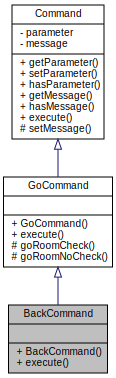
\includegraphics[width=188pt]{classBackCommand__inherit__graph}
\end{center}
\end{figure}


Collaboration diagram for Back\-Command\-:
\nopagebreak
\begin{figure}[H]
\begin{center}
\leavevmode
\includegraphics[width=188pt]{classBackCommand__coll__graph}
\end{center}
\end{figure}
\subsection*{Public Member Functions}
\begin{DoxyCompactItemize}
\item 
\hyperlink{classBackCommand_a779456e24dfb281e5917e936da5fd901}{Back\-Command} ()
\begin{DoxyCompactList}\small\item\em Constructor for \hyperlink{classBackCommand}{Back\-Command}. \end{DoxyCompactList}\item 
boolean \hyperlink{classBackCommand_a1f5b1ecc435b3b03d9d1a880c31c9c7a}{execute} (\hyperlink{classPlayer}{Player} player)  throws Unauthorized\-Exception 
\begin{DoxyCompactList}\small\item\em Go back in a previous room of the player. \end{DoxyCompactList}\end{DoxyCompactItemize}
\subsection*{Additional Inherited Members}


\subsection{Detailed Description}
class \hyperlink{classBackCommand}{Back\-Command} used to go back in a previous \hyperlink{classRoom}{Room}. 

\begin{DoxyAuthor}{Author}
Rémi N\-I\-C\-O\-L\-E 
\end{DoxyAuthor}


Definition at line \hyperlink{BackCommand_8java_source_l00005}{5} of file \hyperlink{BackCommand_8java_source}{Back\-Command.\-java}.



\subsection{Constructor \& Destructor Documentation}
\hypertarget{classBackCommand_a779456e24dfb281e5917e936da5fd901}{\index{Back\-Command@{Back\-Command}!Back\-Command@{Back\-Command}}
\index{Back\-Command@{Back\-Command}!BackCommand@{Back\-Command}}
\subsubsection[{Back\-Command}]{\setlength{\rightskip}{0pt plus 5cm}Back\-Command.\-Back\-Command (
\begin{DoxyParamCaption}
{}
\end{DoxyParamCaption}
)}}\label{classBackCommand_a779456e24dfb281e5917e936da5fd901}


Constructor for \hyperlink{classBackCommand}{Back\-Command}. 



Definition at line \hyperlink{BackCommand_8java_source_l00010}{10} of file \hyperlink{BackCommand_8java_source}{Back\-Command.\-java}.


\begin{DoxyCode}
00010                         \{
00011         super();
00012     \}
\end{DoxyCode}


\subsection{Member Function Documentation}
\hypertarget{classBackCommand_a1f5b1ecc435b3b03d9d1a880c31c9c7a}{\index{Back\-Command@{Back\-Command}!execute@{execute}}
\index{execute@{execute}!BackCommand@{Back\-Command}}
\subsubsection[{execute}]{\setlength{\rightskip}{0pt plus 5cm}boolean Back\-Command.\-execute (
\begin{DoxyParamCaption}
\item[{{\bf Player}}]{player}
\end{DoxyParamCaption}
) throws {\bf Unauthorized\-Exception}}}\label{classBackCommand_a1f5b1ecc435b3b03d9d1a880c31c9c7a}


Go back in a previous room of the player. 


\begin{DoxyParams}{Parameters}
{\em player} & The player that typed the \char`\"{}back\char`\"{} command \\
\hline
\end{DoxyParams}

\begin{DoxyExceptions}{Exceptions}
{\em \hyperlink{classUnauthorizedException}{Unauthorized\-Exception}} & When the user has no previous room \\
\hline
\end{DoxyExceptions}
\begin{DoxyReturn}{Returns}
False because it is not the quit command 
\end{DoxyReturn}


Definition at line \hyperlink{BackCommand_8java_source_l00020}{20} of file \hyperlink{BackCommand_8java_source}{Back\-Command.\-java}.


\begin{DoxyCode}
00020                                                                        \{
00021         \textcolor{keywordflow}{try} \{
00022             super.goRoomCheck(player.getPreviousRoom(), player, \textcolor{keyword}{true});
00023         \} \textcolor{keywordflow}{catch}(\hyperlink{classIllegalArgumentException}{IllegalArgumentException} e)  \{
00024             \textcolor{comment}{// Tried to teleport to null}
00025             \textcolor{keywordflow}{throw} \textcolor{keyword}{new} \hyperlink{classUnauthorizedException}{UnauthorizedException}(\textcolor{stringliteral}{"Awww, that's sweet. The little player
       want to go home.\(\backslash\)n"}
00026                     + \textcolor{stringliteral}{"But we're just getting started!"});
00027         \}
00028         \textcolor{keywordflow}{return} \textcolor{keyword}{false};
00029     \}
\end{DoxyCode}


The documentation for this class was generated from the following file\-:\begin{DoxyCompactItemize}
\item 
\hyperlink{BackCommand_8java}{Back\-Command.\-java}\end{DoxyCompactItemize}

\hypertarget{classBeamerCommand}{\section{Beamer\-Command Class Reference}
\label{classBeamerCommand}\index{Beamer\-Command@{Beamer\-Command}}
}


Inheritance diagram for Beamer\-Command\-:
\nopagebreak
\begin{figure}[H]
\begin{center}
\leavevmode
\includegraphics[width=190pt]{classBeamerCommand__inherit__graph}
\end{center}
\end{figure}


Collaboration diagram for Beamer\-Command\-:
\nopagebreak
\begin{figure}[H]
\begin{center}
\leavevmode
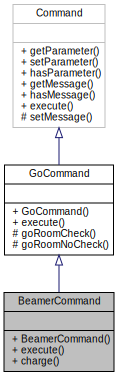
\includegraphics[width=190pt]{classBeamerCommand__coll__graph}
\end{center}
\end{figure}
\subsection*{Public Member Functions}
\begin{DoxyCompactItemize}
\item 
\hyperlink{classBeamerCommand_accb1d84a69588f1b42fba96bf1b32de5}{Beamer\-Command} ()
\item 
boolean \hyperlink{classBeamerCommand_ab28a7d743569841e463b2c0c65cf6eb1}{execute} (\hyperlink{classPlayer}{Player} player)  throws No\-Argument\-Exception,\-Illegal\-Argument\-Exception,\-Unauthorized\-Exception 
\item 
void \hyperlink{classBeamerCommand_a130a572b2ec0532c92ea5033a098b1ac}{charge} (\hyperlink{classPlayer}{Player} player)
\end{DoxyCompactItemize}
\subsection*{Additional Inherited Members}


\subsection{Detailed Description}
class \hyperlink{classBeamerCommand}{Beamer\-Command} used to teleport into a remembered room \begin{DoxyAuthor}{Author}
Rémi N\-I\-C\-O\-L\-E 
\end{DoxyAuthor}


Definition at line \hyperlink{BeamerCommand_8java_source_l00005}{5} of file \hyperlink{BeamerCommand_8java_source}{Beamer\-Command.\-java}.



\subsection{Constructor \& Destructor Documentation}
\hypertarget{classBeamerCommand_accb1d84a69588f1b42fba96bf1b32de5}{\index{Beamer\-Command@{Beamer\-Command}!Beamer\-Command@{Beamer\-Command}}
\index{Beamer\-Command@{Beamer\-Command}!BeamerCommand@{Beamer\-Command}}
\subsubsection[{Beamer\-Command}]{\setlength{\rightskip}{0pt plus 5cm}Beamer\-Command.\-Beamer\-Command (
\begin{DoxyParamCaption}
{}
\end{DoxyParamCaption}
)}}\label{classBeamerCommand_accb1d84a69588f1b42fba96bf1b32de5}
Constructor for \hyperlink{classBeamerCommand}{Beamer\-Command} 

Definition at line \hyperlink{BeamerCommand_8java_source_l00010}{10} of file \hyperlink{BeamerCommand_8java_source}{Beamer\-Command.\-java}.


\begin{DoxyCode}
00010                           \{
00011 
00012     \}
\end{DoxyCode}


\subsection{Member Function Documentation}
\hypertarget{classBeamerCommand_a130a572b2ec0532c92ea5033a098b1ac}{\index{Beamer\-Command@{Beamer\-Command}!charge@{charge}}
\index{charge@{charge}!BeamerCommand@{Beamer\-Command}}
\subsubsection[{charge}]{\setlength{\rightskip}{0pt plus 5cm}void Beamer\-Command.\-charge (
\begin{DoxyParamCaption}
\item[{{\bf Player}}]{player}
\end{DoxyParamCaption}
)}}\label{classBeamerCommand_a130a572b2ec0532c92ea5033a098b1ac}
Remember the current room. 
\begin{DoxyParams}{Parameters}
{\em player} & The player that called this command \\
\hline
\end{DoxyParams}


Definition at line \hyperlink{BeamerCommand_8java_source_l00062}{62} of file \hyperlink{BeamerCommand_8java_source}{Beamer\-Command.\-java}.



References \hyperlink{Player_8java_source_l00151}{Player.\-get\-Beamer\-Room()}.



Referenced by \hyperlink{BeamerCommand_8java_source_l00025}{execute()}.


\begin{DoxyCode}
00062                                       \{
00063         \textcolor{keywordflow}{if}(player.\hyperlink{classPlayer_a9114998742351bf793e093cb198993ca}{getBeamerRoom}() == null)
00064             setMessage(\textcolor{stringliteral}{"Useless room remembered."});
00065         \textcolor{keywordflow}{else}
00066             setMessage(\textcolor{stringliteral}{"Useful room overridden by a useless room."});
00067         player.setBeamerRoom(player.getCurrentRoom());
00068     \}
\end{DoxyCode}


Here is the call graph for this function\-:
\nopagebreak
\begin{figure}[H]
\begin{center}
\leavevmode
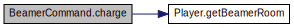
\includegraphics[width=350pt]{classBeamerCommand_a130a572b2ec0532c92ea5033a098b1ac_cgraph}
\end{center}
\end{figure}




Here is the caller graph for this function\-:
\nopagebreak
\begin{figure}[H]
\begin{center}
\leavevmode
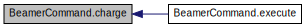
\includegraphics[width=350pt]{classBeamerCommand_a130a572b2ec0532c92ea5033a098b1ac_icgraph}
\end{center}
\end{figure}


\hypertarget{classBeamerCommand_ab28a7d743569841e463b2c0c65cf6eb1}{\index{Beamer\-Command@{Beamer\-Command}!execute@{execute}}
\index{execute@{execute}!BeamerCommand@{Beamer\-Command}}
\subsubsection[{execute}]{\setlength{\rightskip}{0pt plus 5cm}boolean Beamer\-Command.\-execute (
\begin{DoxyParamCaption}
\item[{{\bf Player}}]{player}
\end{DoxyParamCaption}
) throws {\bf No\-Argument\-Exception},{\bf Illegal\-Argument\-Exception},{\bf Unauthorized\-Exception}}}\label{classBeamerCommand_ab28a7d743569841e463b2c0c65cf6eb1}
Teleport to the remembered room or remember a room. It teleports to the remembered room if the command parameter was \char`\"{}teleport\char`\"{}, and it remembers the room if the command parameter was \char`\"{}charge\char`\"{} 
\begin{DoxyParams}{Parameters}
{\em player} & The player that called this command \\
\hline
\end{DoxyParams}

\begin{DoxyExceptions}{Exceptions}
{\em \hyperlink{classNoArgumentException}{No\-Argument\-Exception}} & When the user typed the command without parameter \\
\hline
{\em \hyperlink{classIllegalArgumentException}{Illegal\-Argument\-Exception}} & When the user typed a parameter other than \char`\"{}teleport\char`\"{} or \char`\"{}charge\char`\"{} \\
\hline
{\em \hyperlink{classUnauthorizedException}{Unauthorized\-Exception}} & When the user tries to teleport to null \\
\hline
\end{DoxyExceptions}
\begin{DoxyReturn}{Returns}
False because it is not the quit command 
\end{DoxyReturn}


Definition at line \hyperlink{BeamerCommand_8java_source_l00025}{25} of file \hyperlink{BeamerCommand_8java_source}{Beamer\-Command.\-java}.



References \hyperlink{BeamerCommand_8java_source_l00062}{charge()}.


\begin{DoxyCode}
00025                                                                                                            
               \{
00026         \textcolor{keywordflow}{if}(hasParameter()) \{
00027             \textcolor{keywordflow}{if}(getParameter().equals(\textcolor{stringliteral}{"charge"})) \{
00028                 \hyperlink{classBeamerCommand_a130a572b2ec0532c92ea5033a098b1ac}{charge}(player);
00029                 \textcolor{keywordflow}{return} \textcolor{keyword}{false};
00030             \} \textcolor{keywordflow}{else} \textcolor{keywordflow}{if}(getParameter().equals(\textcolor{stringliteral}{"teleport"})) \{
00031                 teleport(player);
00032                 \textcolor{keywordflow}{return} \textcolor{keyword}{false};
00033             \} \textcolor{keywordflow}{else} \{
00034                 \textcolor{keywordflow}{throw} \textcolor{keyword}{new} \hyperlink{classIllegalArgumentException}{IllegalArgumentException}(\textcolor{stringliteral}{"In order to do that, I may need
       to upgrade. But I don't want to."});
00035             \}
00036         \} \textcolor{keywordflow}{else} 
00037             \textcolor{keywordflow}{throw} \textcolor{keyword}{new} \hyperlink{classNoArgumentException}{NoArgumentException}(\textcolor{stringliteral}{"You can either charge or teleport with the
       beamer.\(\backslash\)nBut that may be too much complicated for you, isn't it?"});
00038     \}
\end{DoxyCode}


Here is the call graph for this function\-:
\nopagebreak
\begin{figure}[H]
\begin{center}
\leavevmode
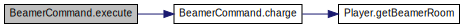
\includegraphics[width=350pt]{classBeamerCommand_ab28a7d743569841e463b2c0c65cf6eb1_cgraph}
\end{center}
\end{figure}




The documentation for this class was generated from the following file\-:\begin{DoxyCompactItemize}
\item 
\hyperlink{BeamerCommand_8java}{Beamer\-Command.\-java}\end{DoxyCompactItemize}

\hypertarget{classCommand}{\section{Command Class Reference}
\label{classCommand}\index{Command@{Command}}
}


Class used to handle a command of one or two words.  




Inheritance diagram for Command\-:
\nopagebreak
\begin{figure}[H]
\begin{center}
\leavevmode
\includegraphics[width=350pt]{classCommand__inherit__graph}
\end{center}
\end{figure}


Collaboration diagram for Command\-:
\nopagebreak
\begin{figure}[H]
\begin{center}
\leavevmode
\includegraphics[width=172pt]{classCommand__coll__graph}
\end{center}
\end{figure}
\subsection*{Public Member Functions}
\begin{DoxyCompactItemize}
\item 
String \hyperlink{classCommand_a1ced3739d546770ba1389e6ce228255e}{get\-Parameter} ()
\begin{DoxyCompactList}\small\item\em Parameter field getter. \end{DoxyCompactList}\item 
void \hyperlink{classCommand_a1301a473bc2a80d40d6ee907c21a1475}{set\-Parameter} (String \hyperlink{classCommand_a02ad27e4576737c16cd78f708188bb54}{parameter})
\begin{DoxyCompactList}\small\item\em Parameter field setter. \end{DoxyCompactList}\item 
boolean \hyperlink{classCommand_a9b042558156d6749566e0fd9d48d3bfe}{has\-Parameter} ()
\begin{DoxyCompactList}\small\item\em Return true if the parameter is null. \end{DoxyCompactList}\item 
String \hyperlink{classCommand_ac3d4abebefb2aea0ce9757bf9c356882}{get\-Message} ()
\begin{DoxyCompactList}\small\item\em Message field getter. \end{DoxyCompactList}\item 
boolean \hyperlink{classCommand_a3d232d33894a20dc81b7627d84f14183}{has\-Message} ()
\begin{DoxyCompactList}\small\item\em Return true if the message is equal to null or \char`\"{}\char`\"{}. \end{DoxyCompactList}\item 
abstract boolean \hyperlink{classCommand_a8e57e3c92529fd3e7e6519fa454422b1}{execute} (\hyperlink{classPlayer}{Player} player)  throws No\-Argument\-Exception,\-Illegal\-Argument\-Exception,\-Unauthorized\-Exception
\begin{DoxyCompactList}\small\item\em Process the command. \end{DoxyCompactList}\end{DoxyCompactItemize}
\subsection*{Protected Member Functions}
\begin{DoxyCompactItemize}
\item 
void \hyperlink{classCommand_a715709d8f0ab65879d79ad1725c96f17}{set\-Message} (String \hyperlink{classCommand_a623fd9ca1e1b03cc35a667bc3e67bc78}{message})
\begin{DoxyCompactList}\small\item\em Message field setter. \end{DoxyCompactList}\end{DoxyCompactItemize}
\subsection*{Private Attributes}
\begin{DoxyCompactItemize}
\item 
String \hyperlink{classCommand_a02ad27e4576737c16cd78f708188bb54}{parameter}
\begin{DoxyCompactList}\small\item\em Parameter for the command. \end{DoxyCompactList}\item 
String \hyperlink{classCommand_a623fd9ca1e1b03cc35a667bc3e67bc78}{message}
\begin{DoxyCompactList}\small\item\em Message to be printed. \end{DoxyCompactList}\end{DoxyCompactItemize}


\subsection{Detailed Description}
Class used to handle a command of one or two words. 

\begin{DoxyAuthor}{Author}
Rémi N\-I\-C\-O\-L\-E 
\end{DoxyAuthor}


Definition at line \hyperlink{Command_8java_source_l00005}{5} of file \hyperlink{Command_8java_source}{Command.\-java}.



\subsection{Member Function Documentation}
\hypertarget{classCommand_a8e57e3c92529fd3e7e6519fa454422b1}{\index{Command@{Command}!execute@{execute}}
\index{execute@{execute}!Command@{Command}}
\subsubsection[{execute}]{\setlength{\rightskip}{0pt plus 5cm}abstract boolean Command.\-execute (
\begin{DoxyParamCaption}
\item[{{\bf Player}}]{player}
\end{DoxyParamCaption}
) throws {\bf No\-Argument\-Exception},{\bf Illegal\-Argument\-Exception},{\bf Unauthorized\-Exception}\hspace{0.3cm}{\ttfamily [abstract]}}}\label{classCommand_a8e57e3c92529fd3e7e6519fa454422b1}


Process the command. 


\begin{DoxyParams}{Parameters}
{\em player} & The player that called this command \\
\hline
\end{DoxyParams}

\begin{DoxyExceptions}{Exceptions}
{\em \hyperlink{classNoArgumentException}{No\-Argument\-Exception}} & When the command needed a parameter but the user didn't specify one \\
\hline
{\em \hyperlink{classIllegalArgumentException}{Illegal\-Argument\-Exception}} & When the user typed a parameter other than the correct ones \\
\hline
{\em \hyperlink{classUnauthorizedException}{Unauthorized\-Exception}} & When the user isn't allowed to do this action \\
\hline
\end{DoxyExceptions}
\hypertarget{classCommand_ac3d4abebefb2aea0ce9757bf9c356882}{\index{Command@{Command}!get\-Message@{get\-Message}}
\index{get\-Message@{get\-Message}!Command@{Command}}
\subsubsection[{get\-Message}]{\setlength{\rightskip}{0pt plus 5cm}String Command.\-get\-Message (
\begin{DoxyParamCaption}
{}
\end{DoxyParamCaption}
)}}\label{classCommand_ac3d4abebefb2aea0ce9757bf9c356882}


Message field getter. 

\begin{DoxyReturn}{Returns}
The message to print to the user 
\end{DoxyReturn}


Definition at line \hyperlink{Command_8java_source_l00057}{57} of file \hyperlink{Command_8java_source}{Command.\-java}.



References \hyperlink{Command_8java_source_l00019}{message}.



Referenced by \hyperlink{TestCommand_8java_source_l00026}{Test\-Command.\-execute()}, \hyperlink{HelpCommand_8java_source_l00028}{Help\-Command.\-execute()}, and \hyperlink{GoCommand_8java_source_l00055}{Go\-Command.\-go\-Room\-No\-Check()}.


\begin{DoxyCode}
00057                                \{
00058         \textcolor{keywordflow}{return} (\hyperlink{classCommand_a623fd9ca1e1b03cc35a667bc3e67bc78}{message} == null)? \textcolor{stringliteral}{""} : \hyperlink{classCommand_a623fd9ca1e1b03cc35a667bc3e67bc78}{message};
00059     \}
\end{DoxyCode}


Here is the caller graph for this function\-:
\nopagebreak
\begin{figure}[H]
\begin{center}
\leavevmode
\includegraphics[width=350pt]{classCommand_ac3d4abebefb2aea0ce9757bf9c356882_icgraph}
\end{center}
\end{figure}


\hypertarget{classCommand_a1ced3739d546770ba1389e6ce228255e}{\index{Command@{Command}!get\-Parameter@{get\-Parameter}}
\index{get\-Parameter@{get\-Parameter}!Command@{Command}}
\subsubsection[{get\-Parameter}]{\setlength{\rightskip}{0pt plus 5cm}String Command.\-get\-Parameter (
\begin{DoxyParamCaption}
{}
\end{DoxyParamCaption}
)}}\label{classCommand_a1ced3739d546770ba1389e6ce228255e}


Parameter field getter. 

\begin{DoxyReturn}{Returns}
The parameter given by the user 
\end{DoxyReturn}


Definition at line \hyperlink{Command_8java_source_l00025}{25} of file \hyperlink{Command_8java_source}{Command.\-java}.



References \hyperlink{Command_8java_source_l00012}{parameter}.



Referenced by \hyperlink{LookCommand_8java_source_l00020}{Look\-Command.\-execute()}, \hyperlink{DropCommand_8java_source_l00021}{Drop\-Command.\-execute()}, \hyperlink{GoCommand_8java_source_l00022}{Go\-Command.\-execute()}, \hyperlink{TakeCommand_8java_source_l00022}{Take\-Command.\-execute()}, \hyperlink{EatCommand_8java_source_l00023}{Eat\-Command.\-execute()}, \hyperlink{BeamerCommand_8java_source_l00025}{Beamer\-Command.\-execute()}, and \hyperlink{TestCommand_8java_source_l00026}{Test\-Command.\-execute()}.


\begin{DoxyCode}
00025                                  \{
00026         \textcolor{keywordflow}{return} \hyperlink{classCommand_a02ad27e4576737c16cd78f708188bb54}{parameter};
00027     \}
\end{DoxyCode}


Here is the caller graph for this function\-:
\nopagebreak
\begin{figure}[H]
\begin{center}
\leavevmode
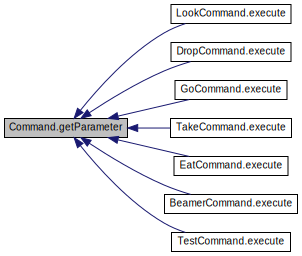
\includegraphics[width=350pt]{classCommand_a1ced3739d546770ba1389e6ce228255e_icgraph}
\end{center}
\end{figure}


\hypertarget{classCommand_a3d232d33894a20dc81b7627d84f14183}{\index{Command@{Command}!has\-Message@{has\-Message}}
\index{has\-Message@{has\-Message}!Command@{Command}}
\subsubsection[{has\-Message}]{\setlength{\rightskip}{0pt plus 5cm}boolean Command.\-has\-Message (
\begin{DoxyParamCaption}
{}
\end{DoxyParamCaption}
)}}\label{classCommand_a3d232d33894a20dc81b7627d84f14183}


Return true if the message is equal to null or \char`\"{}\char`\"{}. 

\begin{DoxyReturn}{Returns}
True if the message is equal to null or \char`\"{}\char`\"{} 
\end{DoxyReturn}


Definition at line \hyperlink{Command_8java_source_l00065}{65} of file \hyperlink{Command_8java_source}{Command.\-java}.



References \hyperlink{Command_8java_source_l00019}{message}.



Referenced by \hyperlink{GoCommand_8java_source_l00055}{Go\-Command.\-go\-Room\-No\-Check()}.


\begin{DoxyCode}
00065                                 \{
00066         \textcolor{keywordflow}{return} (\hyperlink{classCommand_a623fd9ca1e1b03cc35a667bc3e67bc78}{message} == null) ? \textcolor{keyword}{false} : !message.equals(\textcolor{stringliteral}{""});
00067     \}
\end{DoxyCode}


Here is the caller graph for this function\-:
\nopagebreak
\begin{figure}[H]
\begin{center}
\leavevmode
\includegraphics[width=350pt]{classCommand_a3d232d33894a20dc81b7627d84f14183_icgraph}
\end{center}
\end{figure}


\hypertarget{classCommand_a9b042558156d6749566e0fd9d48d3bfe}{\index{Command@{Command}!has\-Parameter@{has\-Parameter}}
\index{has\-Parameter@{has\-Parameter}!Command@{Command}}
\subsubsection[{has\-Parameter}]{\setlength{\rightskip}{0pt plus 5cm}boolean Command.\-has\-Parameter (
\begin{DoxyParamCaption}
{}
\end{DoxyParamCaption}
)}}\label{classCommand_a9b042558156d6749566e0fd9d48d3bfe}


Return true if the parameter is null. 

\begin{DoxyReturn}{Returns}
True if the parameter is null 
\end{DoxyReturn}


Definition at line \hyperlink{Command_8java_source_l00041}{41} of file \hyperlink{Command_8java_source}{Command.\-java}.



References \hyperlink{Command_8java_source_l00012}{parameter}.



Referenced by \hyperlink{LookCommand_8java_source_l00020}{Look\-Command.\-execute()}, \hyperlink{DropCommand_8java_source_l00021}{Drop\-Command.\-execute()}, \hyperlink{GoCommand_8java_source_l00022}{Go\-Command.\-execute()}, \hyperlink{TakeCommand_8java_source_l00022}{Take\-Command.\-execute()}, \hyperlink{EatCommand_8java_source_l00023}{Eat\-Command.\-execute()}, \hyperlink{BeamerCommand_8java_source_l00025}{Beamer\-Command.\-execute()}, and \hyperlink{TestCommand_8java_source_l00026}{Test\-Command.\-execute()}.


\begin{DoxyCode}
00041                                   \{
00042         \textcolor{keywordflow}{return} (\hyperlink{classCommand_a02ad27e4576737c16cd78f708188bb54}{parameter} != null);
00043     \}
\end{DoxyCode}


Here is the caller graph for this function\-:
\nopagebreak
\begin{figure}[H]
\begin{center}
\leavevmode
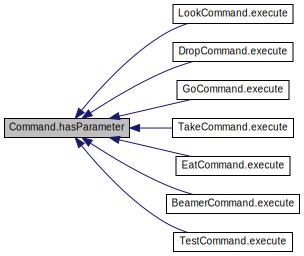
\includegraphics[width=350pt]{classCommand_a9b042558156d6749566e0fd9d48d3bfe_icgraph}
\end{center}
\end{figure}


\hypertarget{classCommand_a715709d8f0ab65879d79ad1725c96f17}{\index{Command@{Command}!set\-Message@{set\-Message}}
\index{set\-Message@{set\-Message}!Command@{Command}}
\subsubsection[{set\-Message}]{\setlength{\rightskip}{0pt plus 5cm}void Command.\-set\-Message (
\begin{DoxyParamCaption}
\item[{String}]{message}
\end{DoxyParamCaption}
)\hspace{0.3cm}{\ttfamily [protected]}}}\label{classCommand_a715709d8f0ab65879d79ad1725c96f17}


Message field setter. 


\begin{DoxyParams}{Parameters}
{\em message} & The message to set \\
\hline
\end{DoxyParams}


Definition at line \hyperlink{Command_8java_source_l00049}{49} of file \hyperlink{Command_8java_source}{Command.\-java}.



References \hyperlink{Command_8java_source_l00019}{message}.



Referenced by \hyperlink{BeamerCommand_8java_source_l00062}{Beamer\-Command.\-charge()}, \hyperlink{InventoryCommand_8java_source_l00019}{Inventory\-Command.\-execute()}, \hyperlink{CreditsCommand_8java_source_l00019}{Credits\-Command.\-execute()}, \hyperlink{LookCommand_8java_source_l00020}{Look\-Command.\-execute()}, \hyperlink{DropCommand_8java_source_l00021}{Drop\-Command.\-execute()}, \hyperlink{TakeCommand_8java_source_l00022}{Take\-Command.\-execute()}, \hyperlink{GoCommand_8java_source_l00022}{Go\-Command.\-execute()}, \hyperlink{EatCommand_8java_source_l00023}{Eat\-Command.\-execute()}, \hyperlink{TestCommand_8java_source_l00026}{Test\-Command.\-execute()}, \hyperlink{HelpCommand_8java_source_l00028}{Help\-Command.\-execute()}, \hyperlink{GoCommand_8java_source_l00055}{Go\-Command.\-go\-Room\-No\-Check()}, and \hyperlink{BeamerCommand_8java_source_l00045}{Beamer\-Command.\-teleport()}.


\begin{DoxyCode}
00049                                               \{
00050         this.message = \hyperlink{classCommand_a623fd9ca1e1b03cc35a667bc3e67bc78}{message};
00051     \}
\end{DoxyCode}


Here is the caller graph for this function\-:
\nopagebreak
\begin{figure}[H]
\begin{center}
\leavevmode
\includegraphics[width=350pt]{classCommand_a715709d8f0ab65879d79ad1725c96f17_icgraph}
\end{center}
\end{figure}


\hypertarget{classCommand_a1301a473bc2a80d40d6ee907c21a1475}{\index{Command@{Command}!set\-Parameter@{set\-Parameter}}
\index{set\-Parameter@{set\-Parameter}!Command@{Command}}
\subsubsection[{set\-Parameter}]{\setlength{\rightskip}{0pt plus 5cm}void Command.\-set\-Parameter (
\begin{DoxyParamCaption}
\item[{String}]{parameter}
\end{DoxyParamCaption}
)}}\label{classCommand_a1301a473bc2a80d40d6ee907c21a1475}


Parameter field setter. 


\begin{DoxyParams}{Parameters}
{\em parameter} & The parameter to set \\
\hline
\end{DoxyParams}


Definition at line \hyperlink{Command_8java_source_l00033}{33} of file \hyperlink{Command_8java_source}{Command.\-java}.



References \hyperlink{Command_8java_source_l00012}{parameter}.


\begin{DoxyCode}
00033                                                \{
00034         this.parameter = \hyperlink{classCommand_a02ad27e4576737c16cd78f708188bb54}{parameter};
00035     \}
\end{DoxyCode}


\subsection{Member Data Documentation}
\hypertarget{classCommand_a623fd9ca1e1b03cc35a667bc3e67bc78}{\index{Command@{Command}!message@{message}}
\index{message@{message}!Command@{Command}}
\subsubsection[{message}]{\setlength{\rightskip}{0pt plus 5cm}String Command.\-message\hspace{0.3cm}{\ttfamily [private]}}}\label{classCommand_a623fd9ca1e1b03cc35a667bc3e67bc78}


Message to be printed. 

This message is printed if and only if the command was successfully processed 

Definition at line \hyperlink{Command_8java_source_l00019}{19} of file \hyperlink{Command_8java_source}{Command.\-java}.



Referenced by \hyperlink{Command_8java_source_l00057}{get\-Message()}, \hyperlink{Command_8java_source_l00065}{has\-Message()}, and \hyperlink{Command_8java_source_l00049}{set\-Message()}.

\hypertarget{classCommand_a02ad27e4576737c16cd78f708188bb54}{\index{Command@{Command}!parameter@{parameter}}
\index{parameter@{parameter}!Command@{Command}}
\subsubsection[{parameter}]{\setlength{\rightskip}{0pt plus 5cm}String Command.\-parameter\hspace{0.3cm}{\ttfamily [private]}}}\label{classCommand_a02ad27e4576737c16cd78f708188bb54}


Parameter for the command. 

It equals to null if there is no parameter. 

Definition at line \hyperlink{Command_8java_source_l00012}{12} of file \hyperlink{Command_8java_source}{Command.\-java}.



Referenced by \hyperlink{Command_8java_source_l00025}{get\-Parameter()}, \hyperlink{Command_8java_source_l00041}{has\-Parameter()}, and \hyperlink{Command_8java_source_l00033}{set\-Parameter()}.



The documentation for this class was generated from the following file\-:\begin{DoxyCompactItemize}
\item 
\hyperlink{Command_8java}{Command.\-java}\end{DoxyCompactItemize}

\hypertarget{enumCommandWord}{\section{Command\-Word Enum Reference}
\label{enumCommandWord}\index{Command\-Word@{Command\-Word}}
}


Representations for all the valid command words for the game.  




Collaboration diagram for Command\-Word\-:
\nopagebreak
\begin{figure}[H]
\begin{center}
\leavevmode
\includegraphics[width=180pt]{enumCommandWord__coll__graph}
\end{center}
\end{figure}
\subsection*{Public Member Functions}
\begin{DoxyCompactItemize}
\item 
\hyperlink{enumCommandWord_a7542ac054c8ee2abf183e01d4e5d2d1f}{Command\-Word} (String \hyperlink{enumCommandWord_ae396b905ac83b5717c56b67e1e47aeef}{command\-String})
\begin{DoxyCompactList}\small\item\em Initialise with the corresponding command word. \end{DoxyCompactList}\item 
String \hyperlink{enumCommandWord_a923828e4531df99a4654d35d160ec486}{to\-String} ()
\end{DoxyCompactItemize}
\subsection*{Public Attributes}
\begin{DoxyCompactItemize}
\item 
\hyperlink{enumCommandWord_ab85d8b5fa5f3890548bff9a1ccfba218}{G\-O} =(\char`\"{}go\char`\"{})
\begin{DoxyCompactList}\small\item\em \char`\"{}go\char`\"{} command representation. \end{DoxyCompactList}\item 
\hyperlink{enumCommandWord_a3309e549607eb8de673c296db55f7517}{B\-A\-C\-K} =(\char`\"{}back\char`\"{})
\begin{DoxyCompactList}\small\item\em \char`\"{}back\char`\"{} command representation. \end{DoxyCompactList}\item 
\hyperlink{enumCommandWord_ab916560f94837341b38c83aa3cf5497f}{B\-E\-A\-M\-E\-R} =(\char`\"{}beamer\char`\"{})
\begin{DoxyCompactList}\small\item\em \char`\"{}beamer\char`\"{} command representation. \end{DoxyCompactList}\item 
\hyperlink{enumCommandWord_ae56e5a1529f673fe19373fed2717cd8c}{L\-O\-O\-K} =(\char`\"{}look\char`\"{})
\begin{DoxyCompactList}\small\item\em \char`\"{}look\char`\"{} command representation. \end{DoxyCompactList}\item 
\hyperlink{enumCommandWord_ac113629c0d6a8ebe3f4050a50d904a17}{T\-A\-K\-E} =(\char`\"{}take\char`\"{})
\begin{DoxyCompactList}\small\item\em \char`\"{}take\char`\"{} command representation. \end{DoxyCompactList}\item 
\hyperlink{enumCommandWord_a68dbdfb6cdd48bebfc70980afad6d453}{D\-R\-O\-P} =(\char`\"{}drop\char`\"{})
\begin{DoxyCompactList}\small\item\em \char`\"{}drop\char`\"{} command representation. \end{DoxyCompactList}\item 
\hyperlink{enumCommandWord_a624e48d45c9a1c4f614c62faa553c855}{I\-N\-V\-E\-N\-T\-O\-R\-Y} =(\char`\"{}inventory\char`\"{})
\begin{DoxyCompactList}\small\item\em \char`\"{}inventory\char`\"{} command representation. \end{DoxyCompactList}\item 
\hyperlink{enumCommandWord_a8a3ddfcc3d3f62697323325970089d95}{E\-A\-T} =(\char`\"{}eat\char`\"{})
\begin{DoxyCompactList}\small\item\em \char`\"{}eat\char`\"{} command representation. \end{DoxyCompactList}\item 
\hyperlink{enumCommandWord_a12071308fc3289269d190f8fe5dd95b4}{T\-E\-S\-T} =(\char`\"{}test\char`\"{})
\begin{DoxyCompactList}\small\item\em \char`\"{}test\char`\"{} command representation. \end{DoxyCompactList}\item 
\hyperlink{enumCommandWord_aa606b7593e9ff8c395e091a0f726e348}{Q\-U\-I\-T} =(\char`\"{}quit\char`\"{})
\begin{DoxyCompactList}\small\item\em \char`\"{}quit\char`\"{} command representation. \end{DoxyCompactList}\item 
\hyperlink{enumCommandWord_a8689456b5990b4dfa2c69427a862784d}{H\-E\-L\-P} =(\char`\"{}help\char`\"{})
\begin{DoxyCompactList}\small\item\em \char`\"{}help\char`\"{} command representation. \end{DoxyCompactList}\item 
\hyperlink{enumCommandWord_aff84c19093cea7bf97301062fe61e0a4}{C\-R\-E\-D\-I\-T\-S} =(\char`\"{}credits\char`\"{})
\begin{DoxyCompactList}\small\item\em \char`\"{}credits\char`\"{} command representation. \end{DoxyCompactList}\item 
\hyperlink{enumCommandWord_a7fac6077f2157eb151a67206fd39c3b9}{U\-N\-K\-N\-O\-W\-N} =(\char`\"{}?\char`\"{})
\begin{DoxyCompactList}\small\item\em Unknown command representation. \end{DoxyCompactList}\end{DoxyCompactItemize}
\subsection*{Private Attributes}
\begin{DoxyCompactItemize}
\item 
String \hyperlink{enumCommandWord_ae396b905ac83b5717c56b67e1e47aeef}{command\-String}
\begin{DoxyCompactList}\small\item\em The String corresponding the the first word of the command. \end{DoxyCompactList}\end{DoxyCompactItemize}


\subsection{Detailed Description}
Representations for all the valid command words for the game. 

\begin{DoxyAuthor}{Author}
Rémi N\-I\-C\-O\-L\-E 
\end{DoxyAuthor}


Definition at line \hyperlink{CommandWord_8java_source_l00005}{5} of file \hyperlink{CommandWord_8java_source}{Command\-Word.\-java}.



\subsection{Constructor \& Destructor Documentation}
\hypertarget{enumCommandWord_a7542ac054c8ee2abf183e01d4e5d2d1f}{\index{Command\-Word@{Command\-Word}!Command\-Word@{Command\-Word}}
\index{Command\-Word@{Command\-Word}!CommandWord@{Command\-Word}}
\subsubsection[{Command\-Word}]{\setlength{\rightskip}{0pt plus 5cm}Command\-Word.\-Command\-Word (
\begin{DoxyParamCaption}
\item[{String}]{command\-String}
\end{DoxyParamCaption}
)}}\label{enumCommandWord_a7542ac054c8ee2abf183e01d4e5d2d1f}


Initialise with the corresponding command word. 


\begin{DoxyParams}{Parameters}
{\em command\-String} & The command string. \\
\hline
\end{DoxyParams}


Definition at line \hyperlink{CommandWord_8java_source_l00070}{70} of file \hyperlink{CommandWord_8java_source}{Command\-Word.\-java}.


\begin{DoxyCode}
00071     \{
00072         this.commandString = \hyperlink{enumCommandWord_ae396b905ac83b5717c56b67e1e47aeef}{commandString};
00073     \}
\end{DoxyCode}


\subsection{Member Function Documentation}
\hypertarget{enumCommandWord_a923828e4531df99a4654d35d160ec486}{\index{Command\-Word@{Command\-Word}!to\-String@{to\-String}}
\index{to\-String@{to\-String}!CommandWord@{Command\-Word}}
\subsubsection[{to\-String}]{\setlength{\rightskip}{0pt plus 5cm}String Command\-Word.\-to\-String (
\begin{DoxyParamCaption}
{}
\end{DoxyParamCaption}
)}}\label{enumCommandWord_a923828e4531df99a4654d35d160ec486}
\begin{DoxyReturn}{Returns}
The command word as a string. 
\end{DoxyReturn}


Definition at line \hyperlink{CommandWord_8java_source_l00078}{78} of file \hyperlink{CommandWord_8java_source}{Command\-Word.\-java}.


\begin{DoxyCode}
00079     \{
00080         \textcolor{keywordflow}{return} \hyperlink{enumCommandWord_ae396b905ac83b5717c56b67e1e47aeef}{commandString};
00081     \}
\end{DoxyCode}


\subsection{Member Data Documentation}
\hypertarget{enumCommandWord_a3309e549607eb8de673c296db55f7517}{\index{Command\-Word@{Command\-Word}!B\-A\-C\-K@{B\-A\-C\-K}}
\index{B\-A\-C\-K@{B\-A\-C\-K}!CommandWord@{Command\-Word}}
\subsubsection[{B\-A\-C\-K}]{\setlength{\rightskip}{0pt plus 5cm}Command\-Word.\-B\-A\-C\-K =(\char`\"{}back\char`\"{})}}\label{enumCommandWord_a3309e549607eb8de673c296db55f7517}


\char`\"{}back\char`\"{} command representation. 



Definition at line \hyperlink{CommandWord_8java_source_l00014}{14} of file \hyperlink{CommandWord_8java_source}{Command\-Word.\-java}.

\hypertarget{enumCommandWord_ab916560f94837341b38c83aa3cf5497f}{\index{Command\-Word@{Command\-Word}!B\-E\-A\-M\-E\-R@{B\-E\-A\-M\-E\-R}}
\index{B\-E\-A\-M\-E\-R@{B\-E\-A\-M\-E\-R}!CommandWord@{Command\-Word}}
\subsubsection[{B\-E\-A\-M\-E\-R}]{\setlength{\rightskip}{0pt plus 5cm}Command\-Word.\-B\-E\-A\-M\-E\-R =(\char`\"{}beamer\char`\"{})}}\label{enumCommandWord_ab916560f94837341b38c83aa3cf5497f}


\char`\"{}beamer\char`\"{} command representation. 



Definition at line \hyperlink{CommandWord_8java_source_l00018}{18} of file \hyperlink{CommandWord_8java_source}{Command\-Word.\-java}.

\hypertarget{enumCommandWord_ae396b905ac83b5717c56b67e1e47aeef}{\index{Command\-Word@{Command\-Word}!command\-String@{command\-String}}
\index{command\-String@{command\-String}!CommandWord@{Command\-Word}}
\subsubsection[{command\-String}]{\setlength{\rightskip}{0pt plus 5cm}String Command\-Word.\-command\-String\hspace{0.3cm}{\ttfamily [private]}}}\label{enumCommandWord_ae396b905ac83b5717c56b67e1e47aeef}


The String corresponding the the first word of the command. 



Definition at line \hyperlink{CommandWord_8java_source_l00063}{63} of file \hyperlink{CommandWord_8java_source}{Command\-Word.\-java}.

\hypertarget{enumCommandWord_aff84c19093cea7bf97301062fe61e0a4}{\index{Command\-Word@{Command\-Word}!C\-R\-E\-D\-I\-T\-S@{C\-R\-E\-D\-I\-T\-S}}
\index{C\-R\-E\-D\-I\-T\-S@{C\-R\-E\-D\-I\-T\-S}!CommandWord@{Command\-Word}}
\subsubsection[{C\-R\-E\-D\-I\-T\-S}]{\setlength{\rightskip}{0pt plus 5cm}Command\-Word.\-C\-R\-E\-D\-I\-T\-S =(\char`\"{}credits\char`\"{})}}\label{enumCommandWord_aff84c19093cea7bf97301062fe61e0a4}


\char`\"{}credits\char`\"{} command representation. 



Definition at line \hyperlink{CommandWord_8java_source_l00054}{54} of file \hyperlink{CommandWord_8java_source}{Command\-Word.\-java}.

\hypertarget{enumCommandWord_a68dbdfb6cdd48bebfc70980afad6d453}{\index{Command\-Word@{Command\-Word}!D\-R\-O\-P@{D\-R\-O\-P}}
\index{D\-R\-O\-P@{D\-R\-O\-P}!CommandWord@{Command\-Word}}
\subsubsection[{D\-R\-O\-P}]{\setlength{\rightskip}{0pt plus 5cm}Command\-Word.\-D\-R\-O\-P =(\char`\"{}drop\char`\"{})}}\label{enumCommandWord_a68dbdfb6cdd48bebfc70980afad6d453}


\char`\"{}drop\char`\"{} command representation. 



Definition at line \hyperlink{CommandWord_8java_source_l00030}{30} of file \hyperlink{CommandWord_8java_source}{Command\-Word.\-java}.

\hypertarget{enumCommandWord_a8a3ddfcc3d3f62697323325970089d95}{\index{Command\-Word@{Command\-Word}!E\-A\-T@{E\-A\-T}}
\index{E\-A\-T@{E\-A\-T}!CommandWord@{Command\-Word}}
\subsubsection[{E\-A\-T}]{\setlength{\rightskip}{0pt plus 5cm}Command\-Word.\-E\-A\-T =(\char`\"{}eat\char`\"{})}}\label{enumCommandWord_a8a3ddfcc3d3f62697323325970089d95}


\char`\"{}eat\char`\"{} command representation. 



Definition at line \hyperlink{CommandWord_8java_source_l00038}{38} of file \hyperlink{CommandWord_8java_source}{Command\-Word.\-java}.

\hypertarget{enumCommandWord_ab85d8b5fa5f3890548bff9a1ccfba218}{\index{Command\-Word@{Command\-Word}!G\-O@{G\-O}}
\index{G\-O@{G\-O}!CommandWord@{Command\-Word}}
\subsubsection[{G\-O}]{\setlength{\rightskip}{0pt plus 5cm}Command\-Word.\-G\-O =(\char`\"{}go\char`\"{})}}\label{enumCommandWord_ab85d8b5fa5f3890548bff9a1ccfba218}


\char`\"{}go\char`\"{} command representation. 



Definition at line \hyperlink{CommandWord_8java_source_l00010}{10} of file \hyperlink{CommandWord_8java_source}{Command\-Word.\-java}.

\hypertarget{enumCommandWord_a8689456b5990b4dfa2c69427a862784d}{\index{Command\-Word@{Command\-Word}!H\-E\-L\-P@{H\-E\-L\-P}}
\index{H\-E\-L\-P@{H\-E\-L\-P}!CommandWord@{Command\-Word}}
\subsubsection[{H\-E\-L\-P}]{\setlength{\rightskip}{0pt plus 5cm}Command\-Word.\-H\-E\-L\-P =(\char`\"{}help\char`\"{})}}\label{enumCommandWord_a8689456b5990b4dfa2c69427a862784d}


\char`\"{}help\char`\"{} command representation. 



Definition at line \hyperlink{CommandWord_8java_source_l00050}{50} of file \hyperlink{CommandWord_8java_source}{Command\-Word.\-java}.

\hypertarget{enumCommandWord_a624e48d45c9a1c4f614c62faa553c855}{\index{Command\-Word@{Command\-Word}!I\-N\-V\-E\-N\-T\-O\-R\-Y@{I\-N\-V\-E\-N\-T\-O\-R\-Y}}
\index{I\-N\-V\-E\-N\-T\-O\-R\-Y@{I\-N\-V\-E\-N\-T\-O\-R\-Y}!CommandWord@{Command\-Word}}
\subsubsection[{I\-N\-V\-E\-N\-T\-O\-R\-Y}]{\setlength{\rightskip}{0pt plus 5cm}Command\-Word.\-I\-N\-V\-E\-N\-T\-O\-R\-Y =(\char`\"{}inventory\char`\"{})}}\label{enumCommandWord_a624e48d45c9a1c4f614c62faa553c855}


\char`\"{}inventory\char`\"{} command representation. 



Definition at line \hyperlink{CommandWord_8java_source_l00034}{34} of file \hyperlink{CommandWord_8java_source}{Command\-Word.\-java}.

\hypertarget{enumCommandWord_ae56e5a1529f673fe19373fed2717cd8c}{\index{Command\-Word@{Command\-Word}!L\-O\-O\-K@{L\-O\-O\-K}}
\index{L\-O\-O\-K@{L\-O\-O\-K}!CommandWord@{Command\-Word}}
\subsubsection[{L\-O\-O\-K}]{\setlength{\rightskip}{0pt plus 5cm}Command\-Word.\-L\-O\-O\-K =(\char`\"{}look\char`\"{})}}\label{enumCommandWord_ae56e5a1529f673fe19373fed2717cd8c}


\char`\"{}look\char`\"{} command representation. 



Definition at line \hyperlink{CommandWord_8java_source_l00022}{22} of file \hyperlink{CommandWord_8java_source}{Command\-Word.\-java}.

\hypertarget{enumCommandWord_aa606b7593e9ff8c395e091a0f726e348}{\index{Command\-Word@{Command\-Word}!Q\-U\-I\-T@{Q\-U\-I\-T}}
\index{Q\-U\-I\-T@{Q\-U\-I\-T}!CommandWord@{Command\-Word}}
\subsubsection[{Q\-U\-I\-T}]{\setlength{\rightskip}{0pt plus 5cm}Command\-Word.\-Q\-U\-I\-T =(\char`\"{}quit\char`\"{})}}\label{enumCommandWord_aa606b7593e9ff8c395e091a0f726e348}


\char`\"{}quit\char`\"{} command representation. 



Definition at line \hyperlink{CommandWord_8java_source_l00046}{46} of file \hyperlink{CommandWord_8java_source}{Command\-Word.\-java}.

\hypertarget{enumCommandWord_ac113629c0d6a8ebe3f4050a50d904a17}{\index{Command\-Word@{Command\-Word}!T\-A\-K\-E@{T\-A\-K\-E}}
\index{T\-A\-K\-E@{T\-A\-K\-E}!CommandWord@{Command\-Word}}
\subsubsection[{T\-A\-K\-E}]{\setlength{\rightskip}{0pt plus 5cm}Command\-Word.\-T\-A\-K\-E =(\char`\"{}take\char`\"{})}}\label{enumCommandWord_ac113629c0d6a8ebe3f4050a50d904a17}


\char`\"{}take\char`\"{} command representation. 



Definition at line \hyperlink{CommandWord_8java_source_l00026}{26} of file \hyperlink{CommandWord_8java_source}{Command\-Word.\-java}.

\hypertarget{enumCommandWord_a12071308fc3289269d190f8fe5dd95b4}{\index{Command\-Word@{Command\-Word}!T\-E\-S\-T@{T\-E\-S\-T}}
\index{T\-E\-S\-T@{T\-E\-S\-T}!CommandWord@{Command\-Word}}
\subsubsection[{T\-E\-S\-T}]{\setlength{\rightskip}{0pt plus 5cm}Command\-Word.\-T\-E\-S\-T =(\char`\"{}test\char`\"{})}}\label{enumCommandWord_a12071308fc3289269d190f8fe5dd95b4}


\char`\"{}test\char`\"{} command representation. 



Definition at line \hyperlink{CommandWord_8java_source_l00042}{42} of file \hyperlink{CommandWord_8java_source}{Command\-Word.\-java}.

\hypertarget{enumCommandWord_a7fac6077f2157eb151a67206fd39c3b9}{\index{Command\-Word@{Command\-Word}!U\-N\-K\-N\-O\-W\-N@{U\-N\-K\-N\-O\-W\-N}}
\index{U\-N\-K\-N\-O\-W\-N@{U\-N\-K\-N\-O\-W\-N}!CommandWord@{Command\-Word}}
\subsubsection[{U\-N\-K\-N\-O\-W\-N}]{\setlength{\rightskip}{0pt plus 5cm}Command\-Word.\-U\-N\-K\-N\-O\-W\-N =(\char`\"{}?\char`\"{})}}\label{enumCommandWord_a7fac6077f2157eb151a67206fd39c3b9}


Unknown command representation. 



Definition at line \hyperlink{CommandWord_8java_source_l00058}{58} of file \hyperlink{CommandWord_8java_source}{Command\-Word.\-java}.



The documentation for this enum was generated from the following file\-:\begin{DoxyCompactItemize}
\item 
\hyperlink{CommandWord_8java}{Command\-Word.\-java}\end{DoxyCompactItemize}

\hypertarget{classCommandWords}{\section{Command\-Words Class Reference}
\label{classCommandWords}\index{Command\-Words@{Command\-Words}}
}


Collaboration diagram for Command\-Words\-:\nopagebreak
\begin{figure}[H]
\begin{center}
\leavevmode
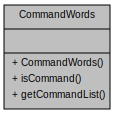
\includegraphics[width=186pt]{classCommandWords__coll__graph}
\end{center}
\end{figure}
\subsection*{Public Member Functions}
\begin{DoxyCompactItemize}
\item 
\hyperlink{classCommandWords_a2d8c096723adb3f822cc001bccd92ed7}{Command\-Words} ()
\item 
boolean \hyperlink{classCommandWords_a98619d278b3fa23fed18b5834f9d20a8}{is\-Command} (String a\-String)
\item 
String \hyperlink{classCommandWords_aa26f54985e39543739e0ae291dcdb8f1}{get\-Command\-List} ()
\end{DoxyCompactItemize}


\subsection{Detailed Description}
Class used to verify the commands given by the user. It contains all known commands and can verify if a String is a known command.

\begin{DoxyAuthor}{Author}
Rémi N\-I\-C\-O\-L\-E 
\end{DoxyAuthor}


Definition at line \hyperlink{CommandWords_8java_source_l00009}{9} of file \hyperlink{CommandWords_8java_source}{Command\-Words.\-java}.



\subsection{Constructor \& Destructor Documentation}
\hypertarget{classCommandWords_a2d8c096723adb3f822cc001bccd92ed7}{\index{Command\-Words@{Command\-Words}!Command\-Words@{Command\-Words}}
\index{Command\-Words@{Command\-Words}!CommandWords@{Command\-Words}}
\subsubsection[{Command\-Words}]{\setlength{\rightskip}{0pt plus 5cm}Command\-Words.\-Command\-Words (
\begin{DoxyParamCaption}
{}
\end{DoxyParamCaption}
)}}\label{classCommandWords_a2d8c096723adb3f822cc001bccd92ed7}
\hyperlink{classCommandWords}{Command\-Words} class constructor. 

Definition at line \hyperlink{CommandWords_8java_source_l00021}{21} of file \hyperlink{CommandWords_8java_source}{Command\-Words.\-java}.


\begin{DoxyCode}
00021                           \{
00022 
00023     \}
\end{DoxyCode}


\subsection{Member Function Documentation}
\hypertarget{classCommandWords_aa26f54985e39543739e0ae291dcdb8f1}{\index{Command\-Words@{Command\-Words}!get\-Command\-List@{get\-Command\-List}}
\index{get\-Command\-List@{get\-Command\-List}!CommandWords@{Command\-Words}}
\subsubsection[{get\-Command\-List}]{\setlength{\rightskip}{0pt plus 5cm}String Command\-Words.\-get\-Command\-List (
\begin{DoxyParamCaption}
{}
\end{DoxyParamCaption}
)}}\label{classCommandWords_aa26f54985e39543739e0ae291dcdb8f1}
Getter for the known\-Commands field. 

Definition at line \hyperlink{CommandWords_8java_source_l00039}{39} of file \hyperlink{CommandWords_8java_source}{Command\-Words.\-java}.


\begin{DoxyCode}
00039                                    \{
00040         StringBuilder commands = \textcolor{keyword}{new} StringBuilder();
00041         \textcolor{keywordflow}{for}(\textcolor{keywordtype}{int} i = 0; i < knownCommands.length; i++) \{
00042             commands.append( knownCommands[i] + \textcolor{stringliteral}{"  "} );
00043         \}
00044         \textcolor{keywordflow}{return} commands.toString();
00045     \}
\end{DoxyCode}
\hypertarget{classCommandWords_a98619d278b3fa23fed18b5834f9d20a8}{\index{Command\-Words@{Command\-Words}!is\-Command@{is\-Command}}
\index{is\-Command@{is\-Command}!CommandWords@{Command\-Words}}
\subsubsection[{is\-Command}]{\setlength{\rightskip}{0pt plus 5cm}boolean Command\-Words.\-is\-Command (
\begin{DoxyParamCaption}
\item[{String}]{a\-String}
\end{DoxyParamCaption}
)}}\label{classCommandWords_a98619d278b3fa23fed18b5834f9d20a8}
Return true if and only if the command is known. 

Definition at line \hyperlink{CommandWords_8java_source_l00028}{28} of file \hyperlink{CommandWords_8java_source}{Command\-Words.\-java}.



Referenced by \hyperlink{Parser_8java_source_l00026}{Parser.\-get\-Command()}.


\begin{DoxyCode}
00028                                              \{
00029         \textcolor{keywordflow}{for}(\textcolor{keywordtype}{int} i = 0; i < knownCommands.length; i++) \{
00030             \textcolor{keywordflow}{if}(knownCommands[i].equals(aString))
00031                 \textcolor{keywordflow}{return} \textcolor{keyword}{true};
00032         \}
00033         \textcolor{keywordflow}{return} \textcolor{keyword}{false};
00034     \}
\end{DoxyCode}


Here is the caller graph for this function\-:\nopagebreak
\begin{figure}[H]
\begin{center}
\leavevmode
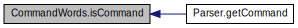
\includegraphics[width=350pt]{classCommandWords_a98619d278b3fa23fed18b5834f9d20a8_icgraph}
\end{center}
\end{figure}




The documentation for this class was generated from the following file\-:\begin{DoxyCompactItemize}
\item 
\hyperlink{CommandWords_8java}{Command\-Words.\-java}\end{DoxyCompactItemize}

\hypertarget{classCreditsCommand}{\section{Credits\-Command Class Reference}
\label{classCreditsCommand}\index{Credits\-Command@{Credits\-Command}}
}


Inheritance diagram for Credits\-Command\-:
\nopagebreak
\begin{figure}[H]
\begin{center}
\leavevmode
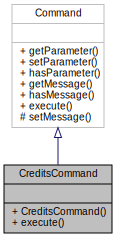
\includegraphics[width=188pt]{classCreditsCommand__inherit__graph}
\end{center}
\end{figure}


Collaboration diagram for Credits\-Command\-:
\nopagebreak
\begin{figure}[H]
\begin{center}
\leavevmode
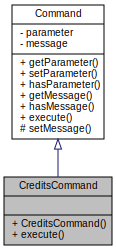
\includegraphics[width=188pt]{classCreditsCommand__coll__graph}
\end{center}
\end{figure}
\subsection*{Public Member Functions}
\begin{DoxyCompactItemize}
\item 
\hyperlink{classCreditsCommand_a3f6edda8e844c13a21a09fc56711b7cd}{Credits\-Command} ()
\item 
boolean \hyperlink{classCreditsCommand_a9b62dcc70ff908b31d84c0c203185889}{execute} (\hyperlink{classPlayer}{Player} player)
\end{DoxyCompactItemize}


\subsection{Detailed Description}
class \hyperlink{classCreditsCommand}{Credits\-Command} used to print the credits of the game \begin{DoxyAuthor}{Author}
Rémi Nicole 
\end{DoxyAuthor}


Definition at line \hyperlink{CreditsCommand_8java_source_l00005}{5} of file \hyperlink{CreditsCommand_8java_source}{Credits\-Command.\-java}.



\subsection{Constructor \& Destructor Documentation}
\hypertarget{classCreditsCommand_a3f6edda8e844c13a21a09fc56711b7cd}{\index{Credits\-Command@{Credits\-Command}!Credits\-Command@{Credits\-Command}}
\index{Credits\-Command@{Credits\-Command}!CreditsCommand@{Credits\-Command}}
\subsubsection[{Credits\-Command}]{\setlength{\rightskip}{0pt plus 5cm}Credits\-Command.\-Credits\-Command (
\begin{DoxyParamCaption}
{}
\end{DoxyParamCaption}
)}}\label{classCreditsCommand_a3f6edda8e844c13a21a09fc56711b7cd}
Constructor for \hyperlink{classCreditsCommand}{Credits\-Command} 

Definition at line \hyperlink{CreditsCommand_8java_source_l00010}{10} of file \hyperlink{CreditsCommand_8java_source}{Credits\-Command.\-java}.


\begin{DoxyCode}
00010                            \{
00011 
00012     \}
\end{DoxyCode}


\subsection{Member Function Documentation}
\hypertarget{classCreditsCommand_a9b62dcc70ff908b31d84c0c203185889}{\index{Credits\-Command@{Credits\-Command}!execute@{execute}}
\index{execute@{execute}!CreditsCommand@{Credits\-Command}}
\subsubsection[{execute}]{\setlength{\rightskip}{0pt plus 5cm}boolean Credits\-Command.\-execute (
\begin{DoxyParamCaption}
\item[{{\bf Player}}]{player}
\end{DoxyParamCaption}
)}}\label{classCreditsCommand_a9b62dcc70ff908b31d84c0c203185889}
Save the credits into the message field. 
\begin{DoxyParams}{Parameters}
{\em player} & The player that called this command \\
\hline
\end{DoxyParams}
\begin{DoxyReturn}{Returns}
False because it is not the quit command 
\end{DoxyReturn}


Definition at line \hyperlink{CreditsCommand_8java_source_l00019}{19} of file \hyperlink{CreditsCommand_8java_source}{Credits\-Command.\-java}.


\begin{DoxyCode}
00019                                           \{
00020         setMessage(\textcolor{stringliteral}{"Temperate rainforest photo (cc-by-nc-nd) : myheimu
       (http://www.fotopedia.com/wiki/Temperate\_rainforest#!/items/flickr-7995237868)\(\backslash\)n"}
00021                 + \textcolor{stringliteral}{"Taiga photo (public domain) : Becker0804
       (https://commons.wikimedia.org/wiki/File:Talkessel\_von\_Werchojansk.JPG)\(\backslash\)n"}
00022                 + \textcolor{stringliteral}{"Alpine tundra photo (public domain) : Zewu
       (https://en.wikipedia.org/wiki/File:Tarfala\_Valley\_-\_Sweden.jpg)\(\backslash\)n"}
00023                 + \textcolor{stringliteral}{"Steppe photo (cc-by-sa) : Matt Lavin
       (http://www.fotopedia.com/wiki/Steppe#!/items/flickr-7495949260)\(\backslash\)n"}
00024                 + \textcolor{stringliteral}{"Lava tube photo : Tim Laman
       (http://science.nationalgeographic.com/science/photos/caves-gallery/#/lava-tube-cave\_1036\_600x450.jpg)\(\backslash\)n"}
00025                 + \textcolor{stringliteral}{"Polar desert photo (cc-by) : Stephen Hudson
       (https://commons.wikimedia.org/wiki/File:AntarcticaDomeCSnow.jpg)\(\backslash\)n"}
00026                 + \textcolor{stringliteral}{"Thar desert photo (cc-by-sa) : Gégard JANOT
       (https://commons.wikimedia.org/wiki/File:D%C3%A9sert\_du\_Rajasthan.jpg)\(\backslash\)n"}
00027                 + \textcolor{stringliteral}{"Savanna photo (public domain) : United States Geological Survey
       (https://commons.wikimedia.org/wiki/File:Oldoinyolengai.jpg)"});
00028         \textcolor{keywordflow}{return} \textcolor{keyword}{false};
00029     \}
\end{DoxyCode}


The documentation for this class was generated from the following file\-:\begin{DoxyCompactItemize}
\item 
\hyperlink{CreditsCommand_8java}{Credits\-Command.\-java}\end{DoxyCompactItemize}

\hypertarget{classDropCommand}{\section{Drop\-Command Class Reference}
\label{classDropCommand}\index{Drop\-Command@{Drop\-Command}}
}


class \hyperlink{classDropCommand}{Drop\-Command} used to make the player drop an \hyperlink{classItem}{Item}  




Inheritance diagram for Drop\-Command\-:
\nopagebreak
\begin{figure}[H]
\begin{center}
\leavevmode
\includegraphics[width=176pt]{classDropCommand__inherit__graph}
\end{center}
\end{figure}


Collaboration diagram for Drop\-Command\-:
\nopagebreak
\begin{figure}[H]
\begin{center}
\leavevmode
\includegraphics[width=176pt]{classDropCommand__coll__graph}
\end{center}
\end{figure}
\subsection*{Public Member Functions}
\begin{DoxyCompactItemize}
\item 
\hyperlink{classDropCommand_a98a8cc14e98c04bed31cd1580e5e3048}{Drop\-Command} ()
\begin{DoxyCompactList}\small\item\em Constructor for \hyperlink{classDropCommand}{Drop\-Command}. \end{DoxyCompactList}\item 
boolean \hyperlink{classDropCommand_a52432de0841ff8eb85d4f115965aecd1}{execute} (\hyperlink{classPlayer}{Player} player)  throws No\-Argument\-Exception,\-Illegal\-Argument\-Exception 
\begin{DoxyCompactList}\small\item\em Drop the \hyperlink{classItem}{Item} through it's name in the parameter field. \end{DoxyCompactList}\end{DoxyCompactItemize}
\subsection*{Additional Inherited Members}


\subsection{Detailed Description}
class \hyperlink{classDropCommand}{Drop\-Command} used to make the player drop an \hyperlink{classItem}{Item} 

\begin{DoxyAuthor}{Author}
Rémi Nicole 
\end{DoxyAuthor}


Definition at line \hyperlink{DropCommand_8java_source_l00005}{5} of file \hyperlink{DropCommand_8java_source}{Drop\-Command.\-java}.



\subsection{Constructor \& Destructor Documentation}
\hypertarget{classDropCommand_a98a8cc14e98c04bed31cd1580e5e3048}{\index{Drop\-Command@{Drop\-Command}!Drop\-Command@{Drop\-Command}}
\index{Drop\-Command@{Drop\-Command}!DropCommand@{Drop\-Command}}
\subsubsection[{Drop\-Command}]{\setlength{\rightskip}{0pt plus 5cm}Drop\-Command.\-Drop\-Command (
\begin{DoxyParamCaption}
{}
\end{DoxyParamCaption}
)}}\label{classDropCommand_a98a8cc14e98c04bed31cd1580e5e3048}


Constructor for \hyperlink{classDropCommand}{Drop\-Command}. 



Definition at line \hyperlink{DropCommand_8java_source_l00010}{10} of file \hyperlink{DropCommand_8java_source}{Drop\-Command.\-java}.


\begin{DoxyCode}
00010                         \{
00011 
00012     \}
\end{DoxyCode}


\subsection{Member Function Documentation}
\hypertarget{classDropCommand_a52432de0841ff8eb85d4f115965aecd1}{\index{Drop\-Command@{Drop\-Command}!execute@{execute}}
\index{execute@{execute}!DropCommand@{Drop\-Command}}
\subsubsection[{execute}]{\setlength{\rightskip}{0pt plus 5cm}boolean Drop\-Command.\-execute (
\begin{DoxyParamCaption}
\item[{{\bf Player}}]{player}
\end{DoxyParamCaption}
) throws {\bf No\-Argument\-Exception},{\bf Illegal\-Argument\-Exception}}}\label{classDropCommand_a52432de0841ff8eb85d4f115965aecd1}


Drop the \hyperlink{classItem}{Item} through it's name in the parameter field. 


\begin{DoxyParams}{Parameters}
{\em player} & The player that called this command \\
\hline
\end{DoxyParams}

\begin{DoxyExceptions}{Exceptions}
{\em \hyperlink{classNoArgumentException}{No\-Argument\-Exception}} & When the user typed the command without parameter \\
\hline
{\em \hyperlink{classIllegalArgumentException}{Illegal\-Argument\-Exception}} & When the user typed a name other than any of the items in the \hyperlink{classPlayer}{Player}'s inventory \\
\hline
\end{DoxyExceptions}
\begin{DoxyReturn}{Returns}
False because it is not the quit command 
\end{DoxyReturn}


Definition at line \hyperlink{DropCommand_8java_source_l00021}{21} of file \hyperlink{DropCommand_8java_source}{Drop\-Command.\-java}.



References \hyperlink{Command_8java_source_l00025}{Command.\-get\-Parameter()}, \hyperlink{Command_8java_source_l00041}{Command.\-has\-Parameter()}, and \hyperlink{Command_8java_source_l00049}{Command.\-set\-Message()}.


\begin{DoxyCode}
00021                                                                                               \{
00022         \textcolor{keywordflow}{if}(\hyperlink{classCommand_a9b042558156d6749566e0fd9d48d3bfe}{hasParameter}()) \{
00023             \textcolor{keywordflow}{if}(player.\hyperlink{classPlayer_a90cb3f05b491eaed668fe54b9258b755}{hasItem}(\hyperlink{classCommand_a1ced3739d546770ba1389e6ce228255e}{getParameter}()))\{
00024                 player.dropObject(\hyperlink{classCommand_a1ced3739d546770ba1389e6ce228255e}{getParameter}());
00025                 \hyperlink{classCommand_a715709d8f0ab65879d79ad1725c96f17}{setMessage}(\textcolor{stringliteral}{"Oh, dear. He took a"} + (((\textcolor{keyword}{new} String(\textcolor{stringliteral}{"aeiouy"})).contains(
      \hyperlink{classCommand_a1ced3739d546770ba1389e6ce228255e}{getParameter}().substring(0,1)))? \textcolor{stringliteral}{"n "} : \textcolor{stringliteral}{" "}) + \hyperlink{classCommand_a1ced3739d546770ba1389e6ce228255e}{getParameter}() + \textcolor{stringliteral}{"."});
00026             \} \textcolor{keywordflow}{else}
00027                 \textcolor{keywordflow}{throw} \textcolor{keyword}{new} \hyperlink{classIllegalArgumentException}{IllegalArgumentException}(\textcolor{stringliteral}{"If you want to drop that, you
       may have a mental disorder. As expected."});
00028         \} \textcolor{keywordflow}{else}
00029             \textcolor{keywordflow}{throw} \textcolor{keyword}{new} \hyperlink{classNoArgumentException}{NoArgumentException}(\textcolor{stringliteral}{"I agree. We both want you to drop dead."});
00030         \textcolor{keywordflow}{return} \textcolor{keyword}{false};
00031     \}
\end{DoxyCode}


Here is the call graph for this function\-:
\nopagebreak
\begin{figure}[H]
\begin{center}
\leavevmode
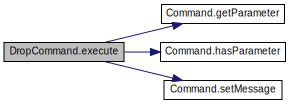
\includegraphics[width=350pt]{classDropCommand_a52432de0841ff8eb85d4f115965aecd1_cgraph}
\end{center}
\end{figure}




The documentation for this class was generated from the following file\-:\begin{DoxyCompactItemize}
\item 
\hyperlink{DropCommand_8java}{Drop\-Command.\-java}\end{DoxyCompactItemize}

\hypertarget{classEatCommand}{\section{Eat\-Command Class Reference}
\label{classEatCommand}\index{Eat\-Command@{Eat\-Command}}
}


Inheritance diagram for Eat\-Command\-:
\nopagebreak
\begin{figure}[H]
\begin{center}
\leavevmode
\includegraphics[width=172pt]{classEatCommand__inherit__graph}
\end{center}
\end{figure}


Collaboration diagram for Eat\-Command\-:
\nopagebreak
\begin{figure}[H]
\begin{center}
\leavevmode
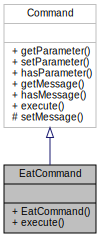
\includegraphics[width=172pt]{classEatCommand__coll__graph}
\end{center}
\end{figure}
\subsection*{Public Member Functions}
\begin{DoxyCompactItemize}
\item 
\hyperlink{classEatCommand_ab142bb810d8beeb46c478148143182e7}{Eat\-Command} ()
\item 
boolean \hyperlink{classEatCommand_ab78ece6b005359a83696998a37f0ae71}{execute} (\hyperlink{classPlayer}{Player} player)  throws No\-Argument\-Exception,\-Illegal\-Argument\-Exception,\-Unauthorized\-Exception 
\end{DoxyCompactItemize}


\subsection{Detailed Description}
class \hyperlink{classEatCommand}{Eat\-Command} used to make the player eat an object. \begin{DoxyAuthor}{Author}
Rémi Nicole 
\end{DoxyAuthor}


Definition at line \hyperlink{EatCommand_8java_source_l00005}{5} of file \hyperlink{EatCommand_8java_source}{Eat\-Command.\-java}.



\subsection{Constructor \& Destructor Documentation}
\hypertarget{classEatCommand_ab142bb810d8beeb46c478148143182e7}{\index{Eat\-Command@{Eat\-Command}!Eat\-Command@{Eat\-Command}}
\index{Eat\-Command@{Eat\-Command}!EatCommand@{Eat\-Command}}
\subsubsection[{Eat\-Command}]{\setlength{\rightskip}{0pt plus 5cm}Eat\-Command.\-Eat\-Command (
\begin{DoxyParamCaption}
{}
\end{DoxyParamCaption}
)}}\label{classEatCommand_ab142bb810d8beeb46c478148143182e7}
Constructor for \hyperlink{classEatCommand}{Eat\-Command} 

Definition at line \hyperlink{EatCommand_8java_source_l00010}{10} of file \hyperlink{EatCommand_8java_source}{Eat\-Command.\-java}.


\begin{DoxyCode}
00010                        \{
00011 
00012     \}
\end{DoxyCode}


\subsection{Member Function Documentation}
\hypertarget{classEatCommand_ab78ece6b005359a83696998a37f0ae71}{\index{Eat\-Command@{Eat\-Command}!execute@{execute}}
\index{execute@{execute}!EatCommand@{Eat\-Command}}
\subsubsection[{execute}]{\setlength{\rightskip}{0pt plus 5cm}boolean Eat\-Command.\-execute (
\begin{DoxyParamCaption}
\item[{{\bf Player}}]{player}
\end{DoxyParamCaption}
) throws {\bf No\-Argument\-Exception},{\bf Illegal\-Argument\-Exception},{\bf Unauthorized\-Exception}}}\label{classEatCommand_ab78ece6b005359a83696998a37f0ae71}
Make the player eat an object. Only the \char`\"{}magiccookie\char`\"{} \hyperlink{classItem}{Item} is eatable 
\begin{DoxyParams}{Parameters}
{\em player} & The player that called this command \\
\hline
\end{DoxyParams}

\begin{DoxyExceptions}{Exceptions}
{\em \hyperlink{classNoArgumentException}{No\-Argument\-Exception}} & When the user typed the command without parameter \\
\hline
{\em \hyperlink{classIllegalArgumentException}{Illegal\-Argument\-Exception}} & When the user typed a name other than any of the items in the \hyperlink{classPlayer}{Player}'s inventory \\
\hline
{\em \hyperlink{classUnauthorizedException}{Unauthorized\-Exception}} & When the user tries to eat a non-\/eatable object \\
\hline
\end{DoxyExceptions}
\begin{DoxyReturn}{Returns}
False because it is not the quit command 
\end{DoxyReturn}


Definition at line \hyperlink{EatCommand_8java_source_l00023}{23} of file \hyperlink{EatCommand_8java_source}{Eat\-Command.\-java}.


\begin{DoxyCode}
00023                                                                                                            
               \{
00024         \textcolor{keywordflow}{if}(hasParameter()) \{
00025             \textcolor{keywordflow}{if}(player.\hyperlink{classPlayer_a90cb3f05b491eaed668fe54b9258b755}{hasItem}(getParameter()))\{
00026                 \textcolor{keywordflow}{if}(getParameter().equals(\textcolor{stringliteral}{"magiccookie"})) \{
00027                     player.eatObject(getParameter());
00028                     player.setMaxWeight(player.getMaxWeight() + 100);
00029                     setMessage(\textcolor{stringliteral}{"You found an out of date \(\backslash\)"magic\(\backslash\)" cookie inside a cave and you just ate
       it.\(\backslash\)nNow you can carry more items. That's logic!"});
00030                 \} \textcolor{keywordflow}{else}
00031                     \textcolor{keywordflow}{throw} \textcolor{keyword}{new} \hyperlink{classUnauthorizedException}{UnauthorizedException}(\textcolor{stringliteral}{"If that's what you eat, I don't
       want to be invited to any of your meals.\(\backslash\)nI'm afraid I can't allow you to do that."});
00032             \} \textcolor{keywordflow}{else} 
00033                 \textcolor{keywordflow}{throw} \textcolor{keyword}{new} \hyperlink{classIllegalArgumentException}{IllegalArgumentException}(\textcolor{stringliteral}{"You don't have that. And I'm
       sure that if you did, it wouldn't be smart to eat that."});
00034         \} \textcolor{keywordflow}{else} 
00035             \textcolor{keywordflow}{throw} \textcolor{keyword}{new} \hyperlink{classNoArgumentException}{NoArgumentException}(\textcolor{stringliteral}{"Eat my shorts?"});
00036         \textcolor{keywordflow}{return} \textcolor{keyword}{false};
00037     \}
\end{DoxyCode}


The documentation for this class was generated from the following file\-:\begin{DoxyCompactItemize}
\item 
\hyperlink{EatCommand_8java}{Eat\-Command.\-java}\end{DoxyCompactItemize}

\hypertarget{classGame}{\section{Game Class Reference}
\label{classGame}\index{Game@{Game}}
}


Collaboration diagram for Game\-:
\nopagebreak
\begin{figure}[H]
\begin{center}
\leavevmode
\includegraphics[width=136pt]{classGame__coll__graph}
\end{center}
\end{figure}
\subsection*{Public Member Functions}
\begin{DoxyCompactItemize}
\item 
\hyperlink{classGame_a2e034e53e9c032964ecd2a831b29a616}{Game} ()
\end{DoxyCompactItemize}
\subsection*{Static Public Member Functions}
\begin{DoxyCompactItemize}
\item 
static void \hyperlink{classGame_ae52595a27ac1b327b05db2129ad81fca}{main} (String\mbox{[}$\,$\mbox{]} args)
\end{DoxyCompactItemize}


\subsection{Detailed Description}
Main class used to instantiate other objects. \begin{DoxyAuthor}{Author}
Rémi N\-I\-C\-O\-L\-E 
\end{DoxyAuthor}


Definition at line \hyperlink{Game_8java_source_l00006}{6} of file \hyperlink{Game_8java_source}{Game.\-java}.



\subsection{Constructor \& Destructor Documentation}
\hypertarget{classGame_a2e034e53e9c032964ecd2a831b29a616}{\index{Game@{Game}!Game@{Game}}
\index{Game@{Game}!Game@{Game}}
\subsubsection[{Game}]{\setlength{\rightskip}{0pt plus 5cm}Game.\-Game (
\begin{DoxyParamCaption}
{}
\end{DoxyParamCaption}
)}}\label{classGame_a2e034e53e9c032964ecd2a831b29a616}
\hyperlink{classGame}{Game} class constructor 

Definition at line \hyperlink{Game_8java_source_l00029}{29} of file \hyperlink{Game_8java_source}{Game.\-java}.



Referenced by \hyperlink{Game_8java_source_l00012}{main()}.


\begin{DoxyCode}
00029                    \{
00030         engine = \textcolor{keyword}{new} \hyperlink{classGameEngine}{GameEngine}();
00031         gui = \textcolor{keyword}{new} \hyperlink{classUserInterface}{UserInterface}(engine);
00032         engine.setGUI(gui);
00033     \}
\end{DoxyCode}


Here is the caller graph for this function\-:
\nopagebreak
\begin{figure}[H]
\begin{center}
\leavevmode
\includegraphics[width=256pt]{classGame_a2e034e53e9c032964ecd2a831b29a616_icgraph}
\end{center}
\end{figure}




\subsection{Member Function Documentation}
\hypertarget{classGame_ae52595a27ac1b327b05db2129ad81fca}{\index{Game@{Game}!main@{main}}
\index{main@{main}!Game@{Game}}
\subsubsection[{main}]{\setlength{\rightskip}{0pt plus 5cm}static void Game.\-main (
\begin{DoxyParamCaption}
\item[{String\mbox{[}$\,$\mbox{]}}]{args}
\end{DoxyParamCaption}
)\hspace{0.3cm}{\ttfamily [static]}}}\label{classGame_ae52595a27ac1b327b05db2129ad81fca}
Main function. 
\begin{DoxyParams}{Parameters}
{\em args} & Command line arguments \\
\hline
\end{DoxyParams}


Definition at line \hyperlink{Game_8java_source_l00012}{12} of file \hyperlink{Game_8java_source}{Game.\-java}.



References \hyperlink{Game_8java_source_l00029}{Game()}.


\begin{DoxyCode}
00012                                            \{
00013         \hyperlink{classGame}{Game} game = \textcolor{keyword}{new} \hyperlink{classGame_a2e034e53e9c032964ecd2a831b29a616}{Game}();
00014     \}
\end{DoxyCode}


Here is the call graph for this function\-:
\nopagebreak
\begin{figure}[H]
\begin{center}
\leavevmode
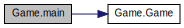
\includegraphics[width=256pt]{classGame_ae52595a27ac1b327b05db2129ad81fca_cgraph}
\end{center}
\end{figure}




The documentation for this class was generated from the following file\-:\begin{DoxyCompactItemize}
\item 
\hyperlink{Game_8java}{Game.\-java}\end{DoxyCompactItemize}

\hypertarget{classGameEngine}{\section{Game\-Engine Class Reference}
\label{classGameEngine}\index{Game\-Engine@{Game\-Engine}}
}


Collaboration diagram for Game\-Engine\-:
\nopagebreak
\begin{figure}[H]
\begin{center}
\leavevmode
\includegraphics[height=550pt]{classGameEngine__coll__graph}
\end{center}
\end{figure}
\subsection*{Public Member Functions}
\begin{DoxyCompactItemize}
\item 
\hyperlink{classGameEngine_a9e8a92f5021a34293060f9aaff4005de}{Game\-Engine} ()
\item 
void \hyperlink{classGameEngine_aec901a5b590b3cd204f196165da5dfb6}{set\-G\-U\-I} (\hyperlink{classUserInterface}{User\-Interface} user\-Interface)
\item 
void \hyperlink{classGameEngine_ad7133885f313fa99bca3bb7cb8272f64}{process\-Command} (String command\-Line)
\end{DoxyCompactItemize}
\subsection*{Private Member Functions}
\begin{DoxyCompactItemize}
\item 
void \hyperlink{classGameEngine_a9a2f3cb921bb19399e357bf14d26425b}{print\-Welcome} ()
\item 
void \hyperlink{classGameEngine_ac32e0d61566d0cca0a1683b5fcf37a00}{create\-Rooms} ()
\item 
void \hyperlink{classGameEngine_a8959e384cc77e69ab0ce9da8ba5057cd}{print\-Help} ()
\item 
void \hyperlink{classGameEngine_a0cc83a912708431a667e73c9a8aa3698}{print\-Credits} ()
\item 
void \hyperlink{classGameEngine_a2ec577574f345764435837fc0204b2e0}{go\-Room} (Command command)
\item 
void \hyperlink{classGameEngine_a09acb51b95ec98aed78d928f91e61a3d}{go\-Room} (\hyperlink{classRoom}{Room} room)
\item 
void \hyperlink{classGameEngine_ae847246e53c53b84787eec490aedf9ad}{go\-Room} (\hyperlink{classRoom}{Room} room, boolean back)
\item 
void \hyperlink{classGameEngine_ac22dcdb540cb27f39597ee4f03ad167a}{go\-Back} ()
\item 
void \hyperlink{classGameEngine_ab620e2e6c8627aba28cc2c33fefe50e3}{look\-Around} (Command command)
\item 
void \hyperlink{classGameEngine_abebbf1bda82aa3ca162f7187a64e41ed}{end\-Game} ()
\item 
void \hyperlink{classGameEngine_a0cfc6fc69e60ffe8a436d04de0938349}{test} (final Command command)
\end{DoxyCompactItemize}
\subsection*{Private Attributes}
\begin{DoxyCompactItemize}
\item 
\hyperlink{classParser}{Parser} \hyperlink{classGameEngine_a2e0d2b1fa2961a930e58e5e6102dc89b}{parser}
\item 
\hyperlink{classRoom}{Room} \hyperlink{classGameEngine_aa08e7cbb458047a2f72ff594d2e230bc}{current\-Room}
\item 
Stack$<$ \hyperlink{classRoom}{Room} $>$ \hyperlink{classGameEngine_a46c905c0610d22223520a8db0e519ec1}{previous\-Rooms}
\item 
\hyperlink{classUserInterface}{User\-Interface} \hyperlink{classGameEngine_a2a7d0bb6183b3f3ef3ee2008926374a0}{gui}
\item 
int \hyperlink{classGameEngine_a308a9926d553d53cb4c56c28588f6c62}{help\-Count}
\end{DoxyCompactItemize}


\subsection{Detailed Description}
Class handling the gameplay for the game. It takes care of room, parser, and room creations and command processing.

\begin{DoxyAuthor}{Author}
Rémi N\-I\-C\-O\-L\-E 
\end{DoxyAuthor}


Definition at line \hyperlink{GameEngine_8java_source_l00011}{11} of file \hyperlink{GameEngine_8java_source}{Game\-Engine.\-java}.



\subsection{Constructor \& Destructor Documentation}
\hypertarget{classGameEngine_a9e8a92f5021a34293060f9aaff4005de}{\index{Game\-Engine@{Game\-Engine}!Game\-Engine@{Game\-Engine}}
\index{Game\-Engine@{Game\-Engine}!GameEngine@{Game\-Engine}}
\subsubsection[{Game\-Engine}]{\setlength{\rightskip}{0pt plus 5cm}Game\-Engine.\-Game\-Engine (
\begin{DoxyParamCaption}
{}
\end{DoxyParamCaption}
)}}\label{classGameEngine_a9e8a92f5021a34293060f9aaff4005de}
\hyperlink{classGameEngine}{Game\-Engine} class constructor. 

Definition at line \hyperlink{GameEngine_8java_source_l00044}{44} of file \hyperlink{GameEngine_8java_source}{Game\-Engine.\-java}.



References \hyperlink{GameEngine_8java_source_l00078}{create\-Rooms()}, \hyperlink{GameEngine_8java_source_l00039}{help\-Count}, \hyperlink{GameEngine_8java_source_l00016}{parser}, and \hyperlink{GameEngine_8java_source_l00026}{previous\-Rooms}.


\begin{DoxyCode}
00044                         \{
00045         \hyperlink{classGameEngine_a2e0d2b1fa2961a930e58e5e6102dc89b}{parser} = \textcolor{keyword}{new} \hyperlink{classParser}{Parser}();
00046         \hyperlink{classGameEngine_ac32e0d61566d0cca0a1683b5fcf37a00}{createRooms}();
00047         \hyperlink{classGameEngine_a46c905c0610d22223520a8db0e519ec1}{previousRooms} = \textcolor{keyword}{new} Stack<Room>();
00048         \hyperlink{classGameEngine_a308a9926d553d53cb4c56c28588f6c62}{helpCount} = 0;
00049     \}
\end{DoxyCode}


Here is the call graph for this function\-:
\nopagebreak
\begin{figure}[H]
\begin{center}
\leavevmode
\includegraphics[width=350pt]{classGameEngine_a9e8a92f5021a34293060f9aaff4005de_cgraph}
\end{center}
\end{figure}




\subsection{Member Function Documentation}
\hypertarget{classGameEngine_ac32e0d61566d0cca0a1683b5fcf37a00}{\index{Game\-Engine@{Game\-Engine}!create\-Rooms@{create\-Rooms}}
\index{create\-Rooms@{create\-Rooms}!GameEngine@{Game\-Engine}}
\subsubsection[{create\-Rooms}]{\setlength{\rightskip}{0pt plus 5cm}void Game\-Engine.\-create\-Rooms (
\begin{DoxyParamCaption}
{}
\end{DoxyParamCaption}
)\hspace{0.3cm}{\ttfamily [private]}}}\label{classGameEngine_ac32e0d61566d0cca0a1683b5fcf37a00}
Create the rooms and link them. 

Definition at line \hyperlink{GameEngine_8java_source_l00078}{78} of file \hyperlink{GameEngine_8java_source}{Game\-Engine.\-java}.



References \hyperlink{GameEngine_8java_source_l00021}{current\-Room}.



Referenced by \hyperlink{GameEngine_8java_source_l00044}{Game\-Engine()}.


\begin{DoxyCode}
00078                                \{
00079         \textcolor{comment}{// create the rooms}
00080         \hyperlink{classRoom}{Room} temperateBroadleaf = \textcolor{keyword}{new} \hyperlink{classRoom}{Room}(\textcolor{stringliteral}{"in temperate forest"}, \textcolor{stringliteral}{"temperatebroadleaf.jpg"});
00081         temperateBroadleaf.addItem(\textcolor{keyword}{new} \hyperlink{classItem}{Item}(\textcolor{stringliteral}{"wand"}, 3, \textcolor{stringliteral}{"just an ordinary wand"}));
00082 
00083         \hyperlink{classRoom}{Room} taiga = \textcolor{keyword}{new} \hyperlink{classRoom}{Room}(\textcolor{stringliteral}{"in a boreal forest"}, \textcolor{stringliteral}{"taiga.jpg"});
00084         taiga.addItem(\textcolor{keyword}{new} \hyperlink{classItem}{Item}(\textcolor{stringliteral}{"snowball"}, 1, \textcolor{stringliteral}{"some weirdly yellowy snowball"}));
00085         taiga.addItem(\textcolor{keyword}{new} \hyperlink{classItem}{Item}(\textcolor{stringliteral}{"bird"}, 6, \textcolor{stringliteral}{"a frozen inert black bird"}));
00086 
00087         \hyperlink{classRoom}{Room} alpineTundra = \textcolor{keyword}{new} \hyperlink{classRoom}{Room}(\textcolor{stringliteral}{"on an alpine mountain"}, \textcolor{stringliteral}{"alpinetundra.jpg"});
00088         alpineTundra.addItem(\textcolor{keyword}{new} \hyperlink{classItem}{Item}(\textcolor{stringliteral}{"rock"}, 15, \textcolor{stringliteral}{"a surprisingly solid magnificent rock"}));
00089         alpineTundra.addItem(\textcolor{keyword}{new} \hyperlink{classItem}{Item}(\textcolor{stringliteral}{"plank"}, 10, \textcolor{stringliteral}{"a plank of wood, maybe from a chalet"}));
00090         alpineTundra.addItem(\textcolor{keyword}{new} \hyperlink{classItem}{Item}(\textcolor{stringliteral}{"snowball"}, 1, \textcolor{stringliteral}{"a snowball. Yes, there is still snow in an alpine
       biome."}));
00091 
00092         \hyperlink{classRoom}{Room} steppe = \textcolor{keyword}{new} \hyperlink{classRoom}{Room}(\textcolor{stringliteral}{"on a vast grass plain"}, \textcolor{stringliteral}{"steppe.jpg"});
00093         steppe.addItem(\textcolor{keyword}{new} \hyperlink{classItem}{Item}(\textcolor{stringliteral}{"grass"}, 1, \textcolor{stringliteral}{"a tuft of yellowish grass. Looking at the grass made you
       look like stupid"}));
00094 
00095         \hyperlink{classRoom}{Room} cave = \textcolor{keyword}{new} \hyperlink{classRoom}{Room}(\textcolor{stringliteral}{"inside a dark cave"}, \textcolor{stringliteral}{"cave.jpg"});
00096 
00097         \hyperlink{classRoom}{Room} polarDesert = \textcolor{keyword}{new} \hyperlink{classRoom}{Room}(\textcolor{stringliteral}{"in a cold polar desert"}, \textcolor{stringliteral}{"polardesert.jpg"});
00098         polarDesert.addItem(\textcolor{keyword}{new} \hyperlink{classItem}{Item}(\textcolor{stringliteral}{"ice"}, 5, \textcolor{stringliteral}{"a little block of ice. But you don't have any drink"}));
00099 
00100         \hyperlink{classRoom}{Room} xericShrublands = \textcolor{keyword}{new} \hyperlink{classRoom}{Room}(\textcolor{stringliteral}{"in a sand desert"}, \textcolor{stringliteral}{"xericshrublands.jpg"});
00101         xericShrublands.addItem(\textcolor{keyword}{new} \hyperlink{classItem}{Item}(\textcolor{stringliteral}{"shrub"}, 10, \textcolor{stringliteral}{"a spicky shrub. Useful if you want to make a
       shruberry"}));
00102 
00103         \hyperlink{classRoom}{Room} savanna = \textcolor{keyword}{new} \hyperlink{classRoom}{Room}(\textcolor{stringliteral}{"in a savanna"}, \textcolor{stringliteral}{"savanna.jpg"});
00104         savanna.addItem(\textcolor{keyword}{new} \hyperlink{classItem}{Item}(\textcolor{stringliteral}{"elephant"}, 1000, \textcolor{stringliteral}{"a huge elephant looking at you, dazed. I bet he's
       smarter than you"}));
00105         savanna.addItem(\textcolor{keyword}{new} \hyperlink{classItem}{Item}(\textcolor{stringliteral}{"grass"}, 1, \textcolor{stringliteral}{"a tuft of yellowish grass. You may have other things to
       do instead of looking at that"}));
00106 
00107         \textcolor{comment}{// initialise room exits}
00108         temperateBroadleaf.setExit(\textcolor{stringliteral}{"east"}, taiga);
00109         temperateBroadleaf.setExit(\textcolor{stringliteral}{"south"}, steppe);
00110 
00111         taiga.setExit(\textcolor{stringliteral}{"west"}, temperateBroadleaf);
00112         taiga.setExit(\textcolor{stringliteral}{"east"}, alpineTundra);
00113         taiga.setExit(\textcolor{stringliteral}{"south"}, cave);
00114 
00115         alpineTundra.setExit(\textcolor{stringliteral}{"west"}, taiga);
00116         alpineTundra.setExit(\textcolor{stringliteral}{"south"}, polarDesert);
00117 
00118         steppe.setExit(\textcolor{stringliteral}{"north"}, temperateBroadleaf);
00119         steppe.setExit(\textcolor{stringliteral}{"east"}, cave);
00120         steppe.setExit(\textcolor{stringliteral}{"south"}, xericShrublands);
00121 
00122         cave.setExit(\textcolor{stringliteral}{"north"}, taiga);
00123         cave.setExit(\textcolor{stringliteral}{"south"}, savanna);
00124         cave.setExit(\textcolor{stringliteral}{"east"}, polarDesert);
00125         cave.setExit(\textcolor{stringliteral}{"west"}, steppe);
00126 
00127         polarDesert.setExit(\textcolor{stringliteral}{"north"}, alpineTundra);
00128         polarDesert.setExit(\textcolor{stringliteral}{"west"}, cave);
00129 
00130         xericShrublands.setExit(\textcolor{stringliteral}{"north"}, steppe);
00131         xericShrublands.setExit(\textcolor{stringliteral}{"east"}, savanna);
00132 
00133         savanna.setExit(\textcolor{stringliteral}{"north"}, cave);
00134         savanna.setExit(\textcolor{stringliteral}{"west"}, xericShrublands);
00135 
00136         \hyperlink{classGameEngine_aa08e7cbb458047a2f72ff594d2e230bc}{currentRoom} = temperateBroadleaf;  \textcolor{comment}{// start game outside}
00137     \}
\end{DoxyCode}


Here is the caller graph for this function\-:
\nopagebreak
\begin{figure}[H]
\begin{center}
\leavevmode
\includegraphics[width=350pt]{classGameEngine_ac32e0d61566d0cca0a1683b5fcf37a00_icgraph}
\end{center}
\end{figure}


\hypertarget{classGameEngine_abebbf1bda82aa3ca162f7187a64e41ed}{\index{Game\-Engine@{Game\-Engine}!end\-Game@{end\-Game}}
\index{end\-Game@{end\-Game}!GameEngine@{Game\-Engine}}
\subsubsection[{end\-Game}]{\setlength{\rightskip}{0pt plus 5cm}void Game\-Engine.\-end\-Game (
\begin{DoxyParamCaption}
{}
\end{DoxyParamCaption}
)\hspace{0.3cm}{\ttfamily [private]}}}\label{classGameEngine_abebbf1bda82aa3ca162f7187a64e41ed}
Print goodbye message and disable gui. 

Definition at line \hyperlink{GameEngine_8java_source_l00276}{276} of file \hyperlink{GameEngine_8java_source}{Game\-Engine.\-java}.



Referenced by \hyperlink{GameEngine_8java_source_l00143}{process\-Command()}.


\begin{DoxyCode}
00276                            \{
00277         gui.println(\textcolor{stringliteral}{"Thank you for playing.  Good bye."});
00278         gui.enable(\textcolor{keyword}{false});
00279     \}
\end{DoxyCode}


Here is the caller graph for this function\-:
\nopagebreak
\begin{figure}[H]
\begin{center}
\leavevmode
\includegraphics[width=350pt]{classGameEngine_abebbf1bda82aa3ca162f7187a64e41ed_icgraph}
\end{center}
\end{figure}


\hypertarget{classGameEngine_ac22dcdb540cb27f39597ee4f03ad167a}{\index{Game\-Engine@{Game\-Engine}!go\-Back@{go\-Back}}
\index{go\-Back@{go\-Back}!GameEngine@{Game\-Engine}}
\subsubsection[{go\-Back}]{\setlength{\rightskip}{0pt plus 5cm}void Game\-Engine.\-go\-Back (
\begin{DoxyParamCaption}
{}
\end{DoxyParamCaption}
)\hspace{0.3cm}{\ttfamily [private]}}}\label{classGameEngine_ac22dcdb540cb27f39597ee4f03ad167a}


Definition at line \hyperlink{GameEngine_8java_source_l00252}{252} of file \hyperlink{GameEngine_8java_source}{Game\-Engine.\-java}.



References \hyperlink{GameEngine_8java_source_l00206}{go\-Room()}, and \hyperlink{GameEngine_8java_source_l00026}{previous\-Rooms}.



Referenced by \hyperlink{GameEngine_8java_source_l00143}{process\-Command()}.


\begin{DoxyCode}
00252                           \{ 
00253         \textcolor{keywordflow}{if}(!\hyperlink{classGameEngine_a46c905c0610d22223520a8db0e519ec1}{previousRooms}.empty()) \{
00254             \hyperlink{classGameEngine_a2ec577574f345764435837fc0204b2e0}{goRoom}(\hyperlink{classGameEngine_a46c905c0610d22223520a8db0e519ec1}{previousRooms}.peek(), \textcolor{keyword}{true});
00255         \} \textcolor{keywordflow}{else} \{
00256             gui.println(\textcolor{stringliteral}{"No previous room"});
00257         \}
00258     \}
\end{DoxyCode}


Here is the call graph for this function\-:
\nopagebreak
\begin{figure}[H]
\begin{center}
\leavevmode
\includegraphics[width=340pt]{classGameEngine_ac22dcdb540cb27f39597ee4f03ad167a_cgraph}
\end{center}
\end{figure}




Here is the caller graph for this function\-:
\nopagebreak
\begin{figure}[H]
\begin{center}
\leavevmode
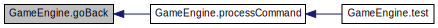
\includegraphics[width=350pt]{classGameEngine_ac22dcdb540cb27f39597ee4f03ad167a_icgraph}
\end{center}
\end{figure}


\hypertarget{classGameEngine_a2ec577574f345764435837fc0204b2e0}{\index{Game\-Engine@{Game\-Engine}!go\-Room@{go\-Room}}
\index{go\-Room@{go\-Room}!GameEngine@{Game\-Engine}}
\subsubsection[{go\-Room}]{\setlength{\rightskip}{0pt plus 5cm}void Game\-Engine.\-go\-Room (
\begin{DoxyParamCaption}
\item[{Command}]{command}
\end{DoxyParamCaption}
)\hspace{0.3cm}{\ttfamily [private]}}}\label{classGameEngine_a2ec577574f345764435837fc0204b2e0}
Go to the given \hyperlink{classRoom}{Room}. 
\begin{DoxyParams}{Parameters}
{\em command} & Command used by the user \\
\hline
\end{DoxyParams}


Definition at line \hyperlink{GameEngine_8java_source_l00206}{206} of file \hyperlink{GameEngine_8java_source}{Game\-Engine.\-java}.



Referenced by \hyperlink{GameEngine_8java_source_l00252}{go\-Back()}, \hyperlink{GameEngine_8java_source_l00226}{go\-Room()}, and \hyperlink{GameEngine_8java_source_l00143}{process\-Command()}.


\begin{DoxyCode}
00206                                          \{
00207         \textcolor{keywordflow}{if}(!command.hasParameter()) \{
00208             \textcolor{comment}{// If there is no second word, we don't know where to go...}
00209             gui.println(\textcolor{stringliteral}{"Go where?"});
00210             \textcolor{keywordflow}{return};
00211         \}
00212 
00213         String direction = command.getParameter();
00214 
00215         \textcolor{comment}{// Try to leave current room.}
00216         \hyperlink{classRoom}{Room} nextRoom = currentRoom.getExit(direction);
00217         \hyperlink{classGameEngine_a2ec577574f345764435837fc0204b2e0}{goRoom}(nextRoom);
00218     \}
\end{DoxyCode}


Here is the caller graph for this function\-:
\nopagebreak
\begin{figure}[H]
\begin{center}
\leavevmode
\includegraphics[width=350pt]{classGameEngine_a2ec577574f345764435837fc0204b2e0_icgraph}
\end{center}
\end{figure}


\hypertarget{classGameEngine_a09acb51b95ec98aed78d928f91e61a3d}{\index{Game\-Engine@{Game\-Engine}!go\-Room@{go\-Room}}
\index{go\-Room@{go\-Room}!GameEngine@{Game\-Engine}}
\subsubsection[{go\-Room}]{\setlength{\rightskip}{0pt plus 5cm}void Game\-Engine.\-go\-Room (
\begin{DoxyParamCaption}
\item[{{\bf Room}}]{room}
\end{DoxyParamCaption}
)\hspace{0.3cm}{\ttfamily [private]}}}\label{classGameEngine_a09acb51b95ec98aed78d928f91e61a3d}
Go to the given \hyperlink{classRoom}{Room}. This function is equivalent to go\-Room(room, false). 
\begin{DoxyParams}{Parameters}
{\em room} & \hyperlink{classRoom}{Room} where the user want to go \\
\hline
\end{DoxyParams}


Definition at line \hyperlink{GameEngine_8java_source_l00226}{226} of file \hyperlink{GameEngine_8java_source}{Game\-Engine.\-java}.



References \hyperlink{GameEngine_8java_source_l00206}{go\-Room()}.


\begin{DoxyCode}
00226                                    \{
00227         \hyperlink{classGameEngine_a2ec577574f345764435837fc0204b2e0}{goRoom}(room, \textcolor{keyword}{false});
00228     \}
\end{DoxyCode}


Here is the call graph for this function\-:
\nopagebreak
\begin{figure}[H]
\begin{center}
\leavevmode
\includegraphics[width=344pt]{classGameEngine_a09acb51b95ec98aed78d928f91e61a3d_cgraph}
\end{center}
\end{figure}


\hypertarget{classGameEngine_ae847246e53c53b84787eec490aedf9ad}{\index{Game\-Engine@{Game\-Engine}!go\-Room@{go\-Room}}
\index{go\-Room@{go\-Room}!GameEngine@{Game\-Engine}}
\subsubsection[{go\-Room}]{\setlength{\rightskip}{0pt plus 5cm}void Game\-Engine.\-go\-Room (
\begin{DoxyParamCaption}
\item[{{\bf Room}}]{room, }
\item[{boolean}]{back}
\end{DoxyParamCaption}
)\hspace{0.3cm}{\ttfamily [private]}}}\label{classGameEngine_ae847246e53c53b84787eec490aedf9ad}
Go to the given \hyperlink{classRoom}{Room}. If the user can't go to the given room, an error message is printed. 
\begin{DoxyParams}{Parameters}
{\em room} & \hyperlink{classRoom}{Room} where the user want to go \\
\hline
{\em back} & true if it is called via the 'back' command \\
\hline
\end{DoxyParams}


Definition at line \hyperlink{GameEngine_8java_source_l00237}{237} of file \hyperlink{GameEngine_8java_source}{Game\-Engine.\-java}.



References \hyperlink{GameEngine_8java_source_l00021}{current\-Room}, \hyperlink{GameEngine_8java_source_l00031}{gui}, and \hyperlink{UserInterface_8java_source_l00069}{User\-Interface.\-show\-Image()}.


\begin{DoxyCode}
00237                                                  \{
00238         \textcolor{keywordflow}{if} (room == null)
00239             gui.println(\textcolor{stringliteral}{"There is no door!"});
00240         \textcolor{keywordflow}{else} \{
00241             \textcolor{keywordflow}{if}(!back)
00242                 previousRooms.push(\hyperlink{classGameEngine_aa08e7cbb458047a2f72ff594d2e230bc}{currentRoom});
00243             \textcolor{keywordflow}{else}
00244                 previousRooms.pop();
00245             \hyperlink{classGameEngine_aa08e7cbb458047a2f72ff594d2e230bc}{currentRoom} = room;
00246             gui.println(currentRoom.getLongDescription());
00247             \textcolor{keywordflow}{if}(\hyperlink{classGameEngine_aa08e7cbb458047a2f72ff594d2e230bc}{currentRoom}.\hyperlink{classRoom_a8177668df4d8be718812934673c42649}{getImageName}() != null)
00248                 \hyperlink{classGameEngine_a2a7d0bb6183b3f3ef3ee2008926374a0}{gui}.\hyperlink{classUserInterface_ab793a0f12878c698ba3e1720a9f86f3b}{showImage}(\hyperlink{classGameEngine_aa08e7cbb458047a2f72ff594d2e230bc}{currentRoom}.\hyperlink{classRoom_a8177668df4d8be718812934673c42649}{getImageName}());
00249         \}
00250     \}
\end{DoxyCode}


Here is the call graph for this function\-:
\nopagebreak
\begin{figure}[H]
\begin{center}
\leavevmode
\includegraphics[width=350pt]{classGameEngine_ae847246e53c53b84787eec490aedf9ad_cgraph}
\end{center}
\end{figure}


\hypertarget{classGameEngine_ab620e2e6c8627aba28cc2c33fefe50e3}{\index{Game\-Engine@{Game\-Engine}!look\-Around@{look\-Around}}
\index{look\-Around@{look\-Around}!GameEngine@{Game\-Engine}}
\subsubsection[{look\-Around}]{\setlength{\rightskip}{0pt plus 5cm}void Game\-Engine.\-look\-Around (
\begin{DoxyParamCaption}
\item[{Command}]{command}
\end{DoxyParamCaption}
)\hspace{0.3cm}{\ttfamily [private]}}}\label{classGameEngine_ab620e2e6c8627aba28cc2c33fefe50e3}
Get the description of the room or a specific object. 
\begin{DoxyParams}{Parameters}
{\em command} & Command used by the user \\
\hline
\end{DoxyParams}


Definition at line \hyperlink{GameEngine_8java_source_l00264}{264} of file \hyperlink{GameEngine_8java_source}{Game\-Engine.\-java}.



References \hyperlink{GameEngine_8java_source_l00021}{current\-Room}, \hyperlink{Room_8java_source_l00100}{Room.\-get\-Long\-Description()}, \hyperlink{GameEngine_8java_source_l00031}{gui}, \hyperlink{Room_8java_source_l00083}{Room.\-has\-Item()}, and \hyperlink{UserInterface_8java_source_l00060}{User\-Interface.\-println()}.



Referenced by \hyperlink{GameEngine_8java_source_l00143}{process\-Command()}.


\begin{DoxyCode}
00264                                              \{
00265         \textcolor{keywordflow}{if}(!command.hasParameter())
00266             \hyperlink{classGameEngine_a2a7d0bb6183b3f3ef3ee2008926374a0}{gui}.\hyperlink{classUserInterface_a79f606b4b1f5d1523e50eea00039ed94}{println}(\hyperlink{classGameEngine_aa08e7cbb458047a2f72ff594d2e230bc}{currentRoom}.\hyperlink{classRoom_a23a25854d7544fb0b41190a4d6bd1322}{getLongDescription}());
00267         \textcolor{keywordflow}{else} \textcolor{keywordflow}{if}(\hyperlink{classGameEngine_aa08e7cbb458047a2f72ff594d2e230bc}{currentRoom}.\hyperlink{classRoom_ad779b367b26018c9f343ca3044c4b54f}{hasItem}(command.getParameter()))
00268             gui.println(\textcolor{stringliteral}{"This is "} + currentRoom.getItem(command.getParameter()).getDescription() + \textcolor{stringliteral}{"."});
00269         \textcolor{keywordflow}{else}
00270             gui.println(\textcolor{stringliteral}{"I'm not sure you want to look at that."});
00271     \}
\end{DoxyCode}


Here is the call graph for this function\-:
\nopagebreak
\begin{figure}[H]
\begin{center}
\leavevmode
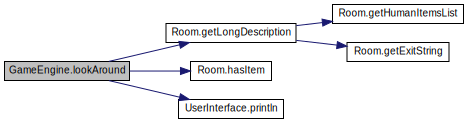
\includegraphics[width=350pt]{classGameEngine_ab620e2e6c8627aba28cc2c33fefe50e3_cgraph}
\end{center}
\end{figure}




Here is the caller graph for this function\-:
\nopagebreak
\begin{figure}[H]
\begin{center}
\leavevmode
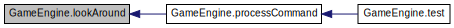
\includegraphics[width=350pt]{classGameEngine_ab620e2e6c8627aba28cc2c33fefe50e3_icgraph}
\end{center}
\end{figure}


\hypertarget{classGameEngine_a0cc83a912708431a667e73c9a8aa3698}{\index{Game\-Engine@{Game\-Engine}!print\-Credits@{print\-Credits}}
\index{print\-Credits@{print\-Credits}!GameEngine@{Game\-Engine}}
\subsubsection[{print\-Credits}]{\setlength{\rightskip}{0pt plus 5cm}void Game\-Engine.\-print\-Credits (
\begin{DoxyParamCaption}
{}
\end{DoxyParamCaption}
)\hspace{0.3cm}{\ttfamily [private]}}}\label{classGameEngine_a0cc83a912708431a667e73c9a8aa3698}
Print the credits for the game. 

Definition at line \hyperlink{GameEngine_8java_source_l00191}{191} of file \hyperlink{GameEngine_8java_source}{Game\-Engine.\-java}.



Referenced by \hyperlink{GameEngine_8java_source_l00143}{process\-Command()}.


\begin{DoxyCode}
00191                                 \{
00192         gui.println(\textcolor{stringliteral}{"Temperate rainforest photo (cc-by-nc-nd) : myheimu
       (http://www.fotopedia.com/wiki/Temperate\_rainforest#!/items/flickr-7995237868)"});
00193         gui.println(\textcolor{stringliteral}{"Taiga photo (public domain) : Becker0804
       (https://commons.wikimedia.org/wiki/File:Talkessel\_von\_Werchojansk.JPG)"});
00194         gui.println(\textcolor{stringliteral}{"Alpine tundra photo (public domain) : Zewu
       (https://en.wikipedia.org/wiki/File:Tarfala\_Valley\_-\_Sweden.jpg)"});
00195         gui.println(\textcolor{stringliteral}{"Steppe photo (cc-by-sa) : Matt Lavin
       (http://www.fotopedia.com/wiki/Steppe#!/items/flickr-7495949260)"});
00196         gui.println(\textcolor{stringliteral}{"Lava tube photo : Tim Laman
       (http://science.nationalgeographic.com/science/photos/caves-gallery/#/lava-tube-cave\_1036\_600x450.jpg)"});
00197         gui.println(\textcolor{stringliteral}{"Polar desert photo (cc-by) : Stephen Hudson
       (https://commons.wikimedia.org/wiki/File:AntarcticaDomeCSnow.jpg)"});
00198         gui.println(\textcolor{stringliteral}{"Thar desert photo (cc-by-sa) : Gégard JANOT
       (https://commons.wikimedia.org/wiki/File:D%C3%A9sert\_du\_Rajasthan.jpg)"});
00199         gui.println(\textcolor{stringliteral}{"Savanna photo (public domain) : United States Geological Survey
       (https://commons.wikimedia.org/wiki/File:Oldoinyolengai.jpg)"});
00200     \}
\end{DoxyCode}


Here is the caller graph for this function\-:
\nopagebreak
\begin{figure}[H]
\begin{center}
\leavevmode
\includegraphics[width=350pt]{classGameEngine_a0cc83a912708431a667e73c9a8aa3698_icgraph}
\end{center}
\end{figure}


\hypertarget{classGameEngine_a8959e384cc77e69ab0ce9da8ba5057cd}{\index{Game\-Engine@{Game\-Engine}!print\-Help@{print\-Help}}
\index{print\-Help@{print\-Help}!GameEngine@{Game\-Engine}}
\subsubsection[{print\-Help}]{\setlength{\rightskip}{0pt plus 5cm}void Game\-Engine.\-print\-Help (
\begin{DoxyParamCaption}
{}
\end{DoxyParamCaption}
)\hspace{0.3cm}{\ttfamily [private]}}}\label{classGameEngine_a8959e384cc77e69ab0ce9da8ba5057cd}
Print user's help. 

Definition at line \hyperlink{GameEngine_8java_source_l00174}{174} of file \hyperlink{GameEngine_8java_source}{Game\-Engine.\-java}.



References \hyperlink{GameEngine_8java_source_l00039}{help\-Count}.



Referenced by \hyperlink{GameEngine_8java_source_l00143}{process\-Command()}.


\begin{DoxyCode}
00174                              \{
00175         \textcolor{keywordflow}{if}(\hyperlink{classGameEngine_a308a9926d553d53cb4c56c28588f6c62}{helpCount} == 0) \{
00176             gui.println(\textcolor{stringliteral}{"Help ? Who needs help ? Only the weak ones."});
00177             \hyperlink{classGameEngine_a308a9926d553d53cb4c56c28588f6c62}{helpCount}++;
00178         \} \textcolor{keywordflow}{else} \{
00179             \textcolor{keywordflow}{if}(\hyperlink{classGameEngine_a308a9926d553d53cb4c56c28588f6c62}{helpCount} == 1) \{
00180                 gui.println(\textcolor{stringliteral}{"All right, all right! If you insist..."});
00181                 \hyperlink{classGameEngine_a308a9926d553d53cb4c56c28588f6c62}{helpCount}++;
00182             \}
00183             gui.println(\textcolor{stringliteral}{"Your command words are: "} + parser.showCommands());
00184             gui.println(\textcolor{stringliteral}{"That will be all."});
00185         \}
00186     \}
\end{DoxyCode}


Here is the caller graph for this function\-:
\nopagebreak
\begin{figure}[H]
\begin{center}
\leavevmode
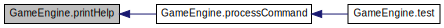
\includegraphics[width=350pt]{classGameEngine_a8959e384cc77e69ab0ce9da8ba5057cd_icgraph}
\end{center}
\end{figure}


\hypertarget{classGameEngine_a9a2f3cb921bb19399e357bf14d26425b}{\index{Game\-Engine@{Game\-Engine}!print\-Welcome@{print\-Welcome}}
\index{print\-Welcome@{print\-Welcome}!GameEngine@{Game\-Engine}}
\subsubsection[{print\-Welcome}]{\setlength{\rightskip}{0pt plus 5cm}void Game\-Engine.\-print\-Welcome (
\begin{DoxyParamCaption}
{}
\end{DoxyParamCaption}
)\hspace{0.3cm}{\ttfamily [private]}}}\label{classGameEngine_a9a2f3cb921bb19399e357bf14d26425b}
Welcome the user at the start of the game. 

Definition at line \hyperlink{GameEngine_8java_source_l00063}{63} of file \hyperlink{GameEngine_8java_source}{Game\-Engine.\-java}.



Referenced by \hyperlink{GameEngine_8java_source_l00055}{set\-G\-U\-I()}.


\begin{DoxyCode}
00063                                 \{
00064         gui.println(\textcolor{stringliteral}{"Greetings human."});
00065         gui.println(\textcolor{stringliteral}{"I see the assassins have failed. Too bad..."});
00066         gui.println(\textcolor{stringliteral}{"You know what they say: if you want something done, do it yourself."});
00067         gui.println(\textcolor{stringliteral}{"At least I can see that you don't remember anything. At last something that I can take
       advantage of."});
00068         gui.println(\textcolor{stringliteral}{"That was predictable, human minds are weak."});
00069         gui.println(\textcolor{stringliteral}{"\(\backslash\)nBecause you're stupid, I will describe you everything that will be around us."});
00070         gui.println(\textcolor{stringliteral}{"Who knows ? Maybe you can turn into something useful. One day. Maybe."});
00071         gui.println(currentRoom.getLongDescription());
00072         gui.showImage(currentRoom.getImageName());
00073     \}
\end{DoxyCode}


Here is the caller graph for this function\-:
\nopagebreak
\begin{figure}[H]
\begin{center}
\leavevmode
\includegraphics[width=350pt]{classGameEngine_a9a2f3cb921bb19399e357bf14d26425b_icgraph}
\end{center}
\end{figure}


\hypertarget{classGameEngine_ad7133885f313fa99bca3bb7cb8272f64}{\index{Game\-Engine@{Game\-Engine}!process\-Command@{process\-Command}}
\index{process\-Command@{process\-Command}!GameEngine@{Game\-Engine}}
\subsubsection[{process\-Command}]{\setlength{\rightskip}{0pt plus 5cm}void Game\-Engine.\-process\-Command (
\begin{DoxyParamCaption}
\item[{String}]{command\-Line}
\end{DoxyParamCaption}
)}}\label{classGameEngine_ad7133885f313fa99bca3bb7cb8272f64}
Process the command. 
\begin{DoxyParams}{Parameters}
{\em command\-Line} & The command to process. \\
\hline
\end{DoxyParams}


Definition at line \hyperlink{GameEngine_8java_source_l00143}{143} of file \hyperlink{GameEngine_8java_source}{Game\-Engine.\-java}.



References \hyperlink{GameEngine_8java_source_l00276}{end\-Game()}, \hyperlink{GameEngine_8java_source_l00252}{go\-Back()}, \hyperlink{GameEngine_8java_source_l00206}{go\-Room()}, \hyperlink{GameEngine_8java_source_l00031}{gui}, \hyperlink{GameEngine_8java_source_l00264}{look\-Around()}, \hyperlink{GameEngine_8java_source_l00191}{print\-Credits()}, \hyperlink{GameEngine_8java_source_l00174}{print\-Help()}, and \hyperlink{UserInterface_8java_source_l00060}{User\-Interface.\-println()}.



Referenced by \hyperlink{GameEngine_8java_source_l00281}{test()}.


\begin{DoxyCode}
00143                                                    \{
00144         gui.println(commandLine);
00145         Command command = parser.getCommand(commandLine);
00146 
00147         \textcolor{keywordflow}{if}(command.isUnknown()) \{
00148             gui.println(\textcolor{stringliteral}{"I don't know what you mean..."});
00149             \textcolor{keywordflow}{return};
00150         \}
00151 
00152         String commandWord = command.getCommandWord();
00153         \textcolor{keywordflow}{if} (commandWord.equals(\textcolor{stringliteral}{"help"}))
00154             \hyperlink{classGameEngine_a8959e384cc77e69ab0ce9da8ba5057cd}{printHelp}();
00155         \textcolor{keywordflow}{else} \textcolor{keywordflow}{if} (commandWord.equals(\textcolor{stringliteral}{"credits"}))
00156             \hyperlink{classGameEngine_a0cc83a912708431a667e73c9a8aa3698}{printCredits}();
00157         \textcolor{keywordflow}{else} \textcolor{keywordflow}{if} (commandWord.equals(\textcolor{stringliteral}{"go"}))
00158             \hyperlink{classGameEngine_a2ec577574f345764435837fc0204b2e0}{goRoom}(command);
00159         \textcolor{keywordflow}{else} \textcolor{keywordflow}{if} (commandWord.equals(\textcolor{stringliteral}{"back"}))
00160             \hyperlink{classGameEngine_ac22dcdb540cb27f39597ee4f03ad167a}{goBack}();
00161         \textcolor{keywordflow}{else} \textcolor{keywordflow}{if} (commandWord.equals(\textcolor{stringliteral}{"look"}))
00162             \hyperlink{classGameEngine_ab620e2e6c8627aba28cc2c33fefe50e3}{lookAround}(command);
00163         \textcolor{keywordflow}{else} \textcolor{keywordflow}{if} (commandWord.equals(\textcolor{stringliteral}{"quit"})) \{
00164             \textcolor{keywordflow}{if}(command.hasParameter())
00165                 \hyperlink{classGameEngine_a2a7d0bb6183b3f3ef3ee2008926374a0}{gui}.\hyperlink{classUserInterface_a79f606b4b1f5d1523e50eea00039ed94}{println}(\textcolor{stringliteral}{"Quit what?"});
00166             \textcolor{keywordflow}{else}
00167                 \hyperlink{classGameEngine_abebbf1bda82aa3ca162f7187a64e41ed}{endGame}();
00168         \}
00169     \}
\end{DoxyCode}


Here is the call graph for this function\-:
\nopagebreak
\begin{figure}[H]
\begin{center}
\leavevmode
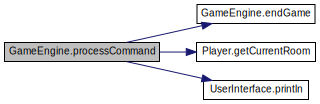
\includegraphics[width=350pt]{classGameEngine_ad7133885f313fa99bca3bb7cb8272f64_cgraph}
\end{center}
\end{figure}




Here is the caller graph for this function\-:
\nopagebreak
\begin{figure}[H]
\begin{center}
\leavevmode
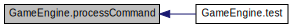
\includegraphics[width=350pt]{classGameEngine_ad7133885f313fa99bca3bb7cb8272f64_icgraph}
\end{center}
\end{figure}


\hypertarget{classGameEngine_aec901a5b590b3cd204f196165da5dfb6}{\index{Game\-Engine@{Game\-Engine}!set\-G\-U\-I@{set\-G\-U\-I}}
\index{set\-G\-U\-I@{set\-G\-U\-I}!GameEngine@{Game\-Engine}}
\subsubsection[{set\-G\-U\-I}]{\setlength{\rightskip}{0pt plus 5cm}void Game\-Engine.\-set\-G\-U\-I (
\begin{DoxyParamCaption}
\item[{{\bf User\-Interface}}]{user\-Interface}
\end{DoxyParamCaption}
)}}\label{classGameEngine_aec901a5b590b3cd204f196165da5dfb6}
Setter for the gui field. \begin{DoxySeeAlso}{See Also}
\hyperlink{classGameEngine_a2a7d0bb6183b3f3ef3ee2008926374a0}{Game\-Engine\-::gui}; 
\end{DoxySeeAlso}


Definition at line \hyperlink{GameEngine_8java_source_l00055}{55} of file \hyperlink{GameEngine_8java_source}{Game\-Engine.\-java}.



References \hyperlink{GameEngine_8java_source_l00031}{gui}, and \hyperlink{GameEngine_8java_source_l00063}{print\-Welcome()}.


\begin{DoxyCode}
00055                                                     \{
00056         \hyperlink{classGameEngine_a2a7d0bb6183b3f3ef3ee2008926374a0}{gui} = userInterface;
00057         \hyperlink{classGameEngine_a9a2f3cb921bb19399e357bf14d26425b}{printWelcome}();
00058     \}
\end{DoxyCode}


Here is the call graph for this function\-:
\nopagebreak
\begin{figure}[H]
\begin{center}
\leavevmode
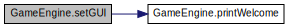
\includegraphics[width=350pt]{classGameEngine_aec901a5b590b3cd204f196165da5dfb6_cgraph}
\end{center}
\end{figure}


\hypertarget{classGameEngine_a0cfc6fc69e60ffe8a436d04de0938349}{\index{Game\-Engine@{Game\-Engine}!test@{test}}
\index{test@{test}!GameEngine@{Game\-Engine}}
\subsubsection[{test}]{\setlength{\rightskip}{0pt plus 5cm}void Game\-Engine.\-test (
\begin{DoxyParamCaption}
\item[{final Command}]{command}
\end{DoxyParamCaption}
)\hspace{0.3cm}{\ttfamily [private]}}}\label{classGameEngine_a0cfc6fc69e60ffe8a436d04de0938349}


Definition at line \hyperlink{GameEngine_8java_source_l00281}{281} of file \hyperlink{GameEngine_8java_source}{Game\-Engine.\-java}.



References \hyperlink{GameEngine_8java_source_l00143}{process\-Command()}.


\begin{DoxyCode}
00281                                              \{
00282         \textcolor{keywordflow}{if}(!command.hasParameter()) \{
00283             gui.println(\textcolor{stringliteral}{"Please specify a file"});
00284             \textcolor{keywordflow}{return};
00285         \} \textcolor{keywordflow}{else} \{
00286             Scanner scan = \textcolor{keyword}{new} Scanner(command.getParameter());
00287             \textcolor{keywordflow}{while}(scan.hasNext()) \{
00288                 \hyperlink{classGameEngine_ad7133885f313fa99bca3bb7cb8272f64}{processCommand}(scan.nextLine());
00289             \}
00290         \}
00291     \}
\end{DoxyCode}


Here is the call graph for this function\-:
\nopagebreak
\begin{figure}[H]
\begin{center}
\leavevmode
\includegraphics[width=350pt]{classGameEngine_a0cfc6fc69e60ffe8a436d04de0938349_cgraph}
\end{center}
\end{figure}




\subsection{Member Data Documentation}
\hypertarget{classGameEngine_aa08e7cbb458047a2f72ff594d2e230bc}{\index{Game\-Engine@{Game\-Engine}!current\-Room@{current\-Room}}
\index{current\-Room@{current\-Room}!GameEngine@{Game\-Engine}}
\subsubsection[{current\-Room}]{\setlength{\rightskip}{0pt plus 5cm}{\bf Room} Game\-Engine.\-current\-Room\hspace{0.3cm}{\ttfamily [private]}}}\label{classGameEngine_aa08e7cbb458047a2f72ff594d2e230bc}
\hyperlink{classRoom}{Room} where the player is currently in. 

Definition at line \hyperlink{GameEngine_8java_source_l00021}{21} of file \hyperlink{GameEngine_8java_source}{Game\-Engine.\-java}.



Referenced by \hyperlink{GameEngine_8java_source_l00078}{create\-Rooms()}, \hyperlink{GameEngine_8java_source_l00237}{go\-Room()}, and \hyperlink{GameEngine_8java_source_l00264}{look\-Around()}.

\hypertarget{classGameEngine_a2a7d0bb6183b3f3ef3ee2008926374a0}{\index{Game\-Engine@{Game\-Engine}!gui@{gui}}
\index{gui@{gui}!GameEngine@{Game\-Engine}}
\subsubsection[{gui}]{\setlength{\rightskip}{0pt plus 5cm}{\bf User\-Interface} Game\-Engine.\-gui\hspace{0.3cm}{\ttfamily [private]}}}\label{classGameEngine_a2a7d0bb6183b3f3ef3ee2008926374a0}
User interface for the game. 

Definition at line \hyperlink{GameEngine_8java_source_l00031}{31} of file \hyperlink{GameEngine_8java_source}{Game\-Engine.\-java}.



Referenced by \hyperlink{GameEngine_8java_source_l00237}{go\-Room()}, \hyperlink{GameEngine_8java_source_l00264}{look\-Around()}, \hyperlink{GameEngine_8java_source_l00143}{process\-Command()}, and \hyperlink{GameEngine_8java_source_l00055}{set\-G\-U\-I()}.

\hypertarget{classGameEngine_a308a9926d553d53cb4c56c28588f6c62}{\index{Game\-Engine@{Game\-Engine}!help\-Count@{help\-Count}}
\index{help\-Count@{help\-Count}!GameEngine@{Game\-Engine}}
\subsubsection[{help\-Count}]{\setlength{\rightskip}{0pt plus 5cm}int Game\-Engine.\-help\-Count\hspace{0.3cm}{\ttfamily [private]}}}\label{classGameEngine_a308a9926d553d53cb4c56c28588f6c62}
Help query counter. It is equal to 0 if the user did not asked for help, 1 if the user asked once the help and 2 if the user asked twice or more for the help 

Definition at line \hyperlink{GameEngine_8java_source_l00039}{39} of file \hyperlink{GameEngine_8java_source}{Game\-Engine.\-java}.



Referenced by \hyperlink{GameEngine_8java_source_l00044}{Game\-Engine()}, and \hyperlink{GameEngine_8java_source_l00174}{print\-Help()}.

\hypertarget{classGameEngine_a2e0d2b1fa2961a930e58e5e6102dc89b}{\index{Game\-Engine@{Game\-Engine}!parser@{parser}}
\index{parser@{parser}!GameEngine@{Game\-Engine}}
\subsubsection[{parser}]{\setlength{\rightskip}{0pt plus 5cm}{\bf Parser} Game\-Engine.\-parser\hspace{0.3cm}{\ttfamily [private]}}}\label{classGameEngine_a2e0d2b1fa2961a930e58e5e6102dc89b}
\hyperlink{classParser}{Parser} for the game. 

Definition at line \hyperlink{GameEngine_8java_source_l00016}{16} of file \hyperlink{GameEngine_8java_source}{Game\-Engine.\-java}.



Referenced by \hyperlink{GameEngine_8java_source_l00044}{Game\-Engine()}.

\hypertarget{classGameEngine_a46c905c0610d22223520a8db0e519ec1}{\index{Game\-Engine@{Game\-Engine}!previous\-Rooms@{previous\-Rooms}}
\index{previous\-Rooms@{previous\-Rooms}!GameEngine@{Game\-Engine}}
\subsubsection[{previous\-Rooms}]{\setlength{\rightskip}{0pt plus 5cm}Stack$<${\bf Room}$>$ Game\-Engine.\-previous\-Rooms\hspace{0.3cm}{\ttfamily [private]}}}\label{classGameEngine_a46c905c0610d22223520a8db0e519ec1}
\hyperlink{classRoom}{Room} where the player was before now. 

Definition at line \hyperlink{GameEngine_8java_source_l00026}{26} of file \hyperlink{GameEngine_8java_source}{Game\-Engine.\-java}.



Referenced by \hyperlink{GameEngine_8java_source_l00044}{Game\-Engine()}, and \hyperlink{GameEngine_8java_source_l00252}{go\-Back()}.



The documentation for this class was generated from the following file\-:\begin{DoxyCompactItemize}
\item 
\hyperlink{GameEngine_8java}{Game\-Engine.\-java}\end{DoxyCompactItemize}

\hypertarget{classGoCommand}{\section{Go\-Command Class Reference}
\label{classGoCommand}\index{Go\-Command@{Go\-Command}}
}


class \hyperlink{classGoCommand}{Go\-Command} used to make the player go to a given \hyperlink{classRoom}{Room}.  




Inheritance diagram for Go\-Command\-:
\nopagebreak
\begin{figure}[H]
\begin{center}
\leavevmode
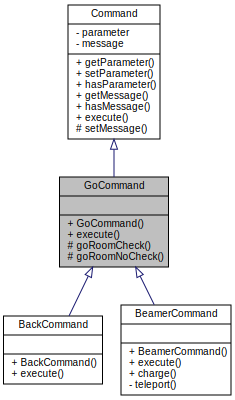
\includegraphics[width=307pt]{classGoCommand__inherit__graph}
\end{center}
\end{figure}


Collaboration diagram for Go\-Command\-:
\nopagebreak
\begin{figure}[H]
\begin{center}
\leavevmode
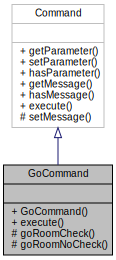
\includegraphics[width=188pt]{classGoCommand__coll__graph}
\end{center}
\end{figure}
\subsection*{Public Member Functions}
\begin{DoxyCompactItemize}
\item 
\hyperlink{classGoCommand_a30d6bd5c2284b97e76ebe702e1cb1d55}{Go\-Command} ()
\begin{DoxyCompactList}\small\item\em Constructor for \hyperlink{classGoCommand}{Go\-Command}. \end{DoxyCompactList}\item 
boolean \hyperlink{classGoCommand_a77a61c2a3b89dca45b51e06f3bcb3ba7}{execute} (\hyperlink{classPlayer}{Player} player)  throws No\-Argument\-Exception,\-Illegal\-Argument\-Exception,\-Unauthorized\-Exception 
\begin{DoxyCompactList}\small\item\em Make the player go to the \hyperlink{classRoom}{Room} through it's direction in the parameter field. \end{DoxyCompactList}\end{DoxyCompactItemize}
\subsection*{Protected Member Functions}
\begin{DoxyCompactItemize}
\item 
void \hyperlink{classGoCommand_a1fce2ad8ed1faf41fa300064585b3616}{go\-Room\-Check} (\hyperlink{classRoom}{Room} room, \hyperlink{classPlayer}{Player} player, boolean back)  throws Illegal\-Argument\-Exception,\-Unauthorized\-Exception 
\begin{DoxyCompactList}\small\item\em Check if the wanted \hyperlink{classRoom}{Room} is connected to the current \hyperlink{classRoom}{Room} and go to this room. \end{DoxyCompactList}\item 
void \hyperlink{classGoCommand_a3149bf695c19b78c39cfc4dadece7846}{go\-Room\-No\-Check} (\hyperlink{classRoom}{Room} room, \hyperlink{classPlayer}{Player} player, boolean back)  throws Illegal\-Argument\-Exception 
\begin{DoxyCompactList}\small\item\em Go to the \hyperlink{classRoom}{Room} without checking. \end{DoxyCompactList}\end{DoxyCompactItemize}


\subsection{Detailed Description}
class \hyperlink{classGoCommand}{Go\-Command} used to make the player go to a given \hyperlink{classRoom}{Room}. 

\begin{DoxyAuthor}{Author}
Rémi Nicole 
\end{DoxyAuthor}


Definition at line \hyperlink{GoCommand_8java_source_l00005}{5} of file \hyperlink{GoCommand_8java_source}{Go\-Command.\-java}.



\subsection{Constructor \& Destructor Documentation}
\hypertarget{classGoCommand_a30d6bd5c2284b97e76ebe702e1cb1d55}{\index{Go\-Command@{Go\-Command}!Go\-Command@{Go\-Command}}
\index{Go\-Command@{Go\-Command}!GoCommand@{Go\-Command}}
\subsubsection[{Go\-Command}]{\setlength{\rightskip}{0pt plus 5cm}Go\-Command.\-Go\-Command (
\begin{DoxyParamCaption}
{}
\end{DoxyParamCaption}
)}}\label{classGoCommand_a30d6bd5c2284b97e76ebe702e1cb1d55}


Constructor for \hyperlink{classGoCommand}{Go\-Command}. 



Definition at line \hyperlink{GoCommand_8java_source_l00010}{10} of file \hyperlink{GoCommand_8java_source}{Go\-Command.\-java}.


\begin{DoxyCode}
00010                       \{
00011 
00012     \}
\end{DoxyCode}


\subsection{Member Function Documentation}
\hypertarget{classGoCommand_a77a61c2a3b89dca45b51e06f3bcb3ba7}{\index{Go\-Command@{Go\-Command}!execute@{execute}}
\index{execute@{execute}!GoCommand@{Go\-Command}}
\subsubsection[{execute}]{\setlength{\rightskip}{0pt plus 5cm}boolean Go\-Command.\-execute (
\begin{DoxyParamCaption}
\item[{{\bf Player}}]{player}
\end{DoxyParamCaption}
) throws {\bf No\-Argument\-Exception},{\bf Illegal\-Argument\-Exception},{\bf Unauthorized\-Exception}}}\label{classGoCommand_a77a61c2a3b89dca45b51e06f3bcb3ba7}


Make the player go to the \hyperlink{classRoom}{Room} through it's direction in the parameter field. 


\begin{DoxyParams}{Parameters}
{\em player} & The player that called this command \\
\hline
\end{DoxyParams}

\begin{DoxyExceptions}{Exceptions}
{\em \hyperlink{classNoArgumentException}{No\-Argument\-Exception}} & When the user typed the command without parameter \\
\hline
{\em \hyperlink{classIllegalArgumentException}{Illegal\-Argument\-Exception}} & When the user typed a parameter other than an available exit direction \\
\hline
{\em \hyperlink{classUnauthorizedException}{Unauthorized\-Exception}} & When the user isn't allowed to go to the given \hyperlink{classRoom}{Room} \\
\hline
\end{DoxyExceptions}
\begin{DoxyReturn}{Returns}
False because it is not the quit command 
\end{DoxyReturn}


Definition at line \hyperlink{GoCommand_8java_source_l00022}{22} of file \hyperlink{GoCommand_8java_source}{Go\-Command.\-java}.



References \hyperlink{Command_8java_source_l00025}{Command.\-get\-Parameter()}, \hyperlink{GoCommand_8java_source_l00040}{go\-Room\-Check()}, \hyperlink{Command_8java_source_l00041}{Command.\-has\-Parameter()}, and \hyperlink{Command_8java_source_l00049}{Command.\-set\-Message()}.


\begin{DoxyCode}
00022                                                                                                            
               \{
00023         \hyperlink{classCommand_a715709d8f0ab65879d79ad1725c96f17}{setMessage}(\textcolor{stringliteral}{""});
00024         \textcolor{keywordflow}{if}(\hyperlink{classCommand_a9b042558156d6749566e0fd9d48d3bfe}{hasParameter}()) \{
00025             \hyperlink{classGoCommand_a1fce2ad8ed1faf41fa300064585b3616}{goRoomCheck}(player.\hyperlink{classPlayer_a3a3107df50fc4e35e8c0f46c3f776ce6}{getCurrentRoom}().getExit(
      \hyperlink{classCommand_a1ced3739d546770ba1389e6ce228255e}{getParameter}()), player, \textcolor{keyword}{false});
00026         \} \textcolor{keywordflow}{else} \{
00027             \textcolor{keywordflow}{throw} \textcolor{keyword}{new} \hyperlink{classNoArgumentException}{NoArgumentException}(\textcolor{stringliteral}{"If you were clever, I would have thought that
       it was a existential question.\(\backslash\)nBut that is not the case and I cannot allow you to go nowhere"});
00028         \}
00029         \textcolor{keywordflow}{return} \textcolor{keyword}{false};
00030     \}
\end{DoxyCode}


Here is the call graph for this function\-:
\nopagebreak
\begin{figure}[H]
\begin{center}
\leavevmode
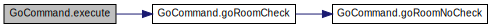
\includegraphics[width=350pt]{classGoCommand_a77a61c2a3b89dca45b51e06f3bcb3ba7_cgraph}
\end{center}
\end{figure}


\hypertarget{classGoCommand_a1fce2ad8ed1faf41fa300064585b3616}{\index{Go\-Command@{Go\-Command}!go\-Room\-Check@{go\-Room\-Check}}
\index{go\-Room\-Check@{go\-Room\-Check}!GoCommand@{Go\-Command}}
\subsubsection[{go\-Room\-Check}]{\setlength{\rightskip}{0pt plus 5cm}void Go\-Command.\-go\-Room\-Check (
\begin{DoxyParamCaption}
\item[{{\bf Room}}]{room, }
\item[{{\bf Player}}]{player, }
\item[{boolean}]{back}
\end{DoxyParamCaption}
) throws {\bf Illegal\-Argument\-Exception},{\bf Unauthorized\-Exception}\hspace{0.3cm}{\ttfamily [protected]}}}\label{classGoCommand_a1fce2ad8ed1faf41fa300064585b3616}


Check if the wanted \hyperlink{classRoom}{Room} is connected to the current \hyperlink{classRoom}{Room} and go to this room. 


\begin{DoxyParams}{Parameters}
{\em room} & \hyperlink{classRoom}{Room} where the user want to go \\
\hline
{\em player} & The player that called this command \\
\hline
{\em back} & true if it is called via the 'back' command \\
\hline
\end{DoxyParams}

\begin{DoxyExceptions}{Exceptions}
{\em \hyperlink{classIllegalArgumentException}{Illegal\-Argument\-Exception}} & When the user tries to go to null \\
\hline
{\em \hyperlink{classUnauthorizedException}{Unauthorized\-Exception}} & When the user isn't allowed to go to the given \hyperlink{classRoom}{Room} \\
\hline
\end{DoxyExceptions}


Definition at line \hyperlink{GoCommand_8java_source_l00040}{40} of file \hyperlink{GoCommand_8java_source}{Go\-Command.\-java}.



References \hyperlink{GoCommand_8java_source_l00055}{go\-Room\-No\-Check()}.



Referenced by \hyperlink{GoCommand_8java_source_l00022}{execute()}.


\begin{DoxyCode}
00040                                                                                                            
                        \{
00041         \textcolor{keywordflow}{if}(player.\hyperlink{classPlayer_a3a3107df50fc4e35e8c0f46c3f776ce6}{getCurrentRoom}().isExit(room)) \{
00042             \hyperlink{classGoCommand_a3149bf695c19b78c39cfc4dadece7846}{goRoomNoCheck}(room, player, back);
00043         \} \textcolor{keywordflow}{else} \{
00044             \textcolor{keywordflow}{throw} \textcolor{keyword}{new} \hyperlink{classUnauthorizedException}{UnauthorizedException}(\textcolor{stringliteral}{"I'm sorry but you can't pass through
       walls."});
00045         \}
00046     \}
\end{DoxyCode}


Here is the call graph for this function\-:
\nopagebreak
\begin{figure}[H]
\begin{center}
\leavevmode
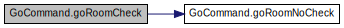
\includegraphics[width=350pt]{classGoCommand_a1fce2ad8ed1faf41fa300064585b3616_cgraph}
\end{center}
\end{figure}




Here is the caller graph for this function\-:
\nopagebreak
\begin{figure}[H]
\begin{center}
\leavevmode
\includegraphics[width=350pt]{classGoCommand_a1fce2ad8ed1faf41fa300064585b3616_icgraph}
\end{center}
\end{figure}


\hypertarget{classGoCommand_a3149bf695c19b78c39cfc4dadece7846}{\index{Go\-Command@{Go\-Command}!go\-Room\-No\-Check@{go\-Room\-No\-Check}}
\index{go\-Room\-No\-Check@{go\-Room\-No\-Check}!GoCommand@{Go\-Command}}
\subsubsection[{go\-Room\-No\-Check}]{\setlength{\rightskip}{0pt plus 5cm}void Go\-Command.\-go\-Room\-No\-Check (
\begin{DoxyParamCaption}
\item[{{\bf Room}}]{room, }
\item[{{\bf Player}}]{player, }
\item[{boolean}]{back}
\end{DoxyParamCaption}
) throws {\bf Illegal\-Argument\-Exception}\hspace{0.3cm}{\ttfamily [protected]}}}\label{classGoCommand_a3149bf695c19b78c39cfc4dadece7846}


Go to the \hyperlink{classRoom}{Room} without checking. 


\begin{DoxyParams}{Parameters}
{\em room} & \hyperlink{classRoom}{Room} where the user want to go \\
\hline
{\em player} & The player that called this command \\
\hline
{\em back} & true if it is called via the 'back' command \\
\hline
\end{DoxyParams}

\begin{DoxyExceptions}{Exceptions}
{\em \hyperlink{classIllegalArgumentException}{Illegal\-Argument\-Exception}} & When the user tries to go to null \\
\hline
\end{DoxyExceptions}


Definition at line \hyperlink{GoCommand_8java_source_l00055}{55} of file \hyperlink{GoCommand_8java_source}{Go\-Command.\-java}.



References \hyperlink{Command_8java_source_l00057}{Command.\-get\-Message()}, \hyperlink{Command_8java_source_l00065}{Command.\-has\-Message()}, and \hyperlink{Command_8java_source_l00049}{Command.\-set\-Message()}.



Referenced by \hyperlink{GoCommand_8java_source_l00040}{go\-Room\-Check()}, and \hyperlink{BeamerCommand_8java_source_l00045}{Beamer\-Command.\-teleport()}.


\begin{DoxyCode}
00055                                                                                                          \{
00056         \textcolor{keywordflow}{if}(room != null) \{
00057             \textcolor{keywordflow}{if}(!back)
00058                 player.pushForward();
00059             \textcolor{keywordflow}{else}
00060                 player.popPreviousRooms();
00061             player.goRoom(room);
00062             \hyperlink{classCommand_a715709d8f0ab65879d79ad1725c96f17}{setMessage}(((\hyperlink{classCommand_a3d232d33894a20dc81b7627d84f14183}{hasMessage}()) ? \hyperlink{classCommand_ac3d4abebefb2aea0ce9757bf9c356882}{getMessage}() + \textcolor{stringliteral}{"\(\backslash\)n"} : \textcolor{stringliteral}{""}) + room.
      \hyperlink{classRoom_a23a25854d7544fb0b41190a4d6bd1322}{getLongDescription}());
00063         \} \textcolor{keywordflow}{else}
00064             \textcolor{keywordflow}{throw} \textcolor{keyword}{new} \hyperlink{classIllegalArgumentException}{IllegalArgumentException}(\textcolor{stringliteral}{"This is a wall, not a door!"});
00065     \}
\end{DoxyCode}


Here is the call graph for this function\-:
\nopagebreak
\begin{figure}[H]
\begin{center}
\leavevmode
\includegraphics[width=350pt]{classGoCommand_a3149bf695c19b78c39cfc4dadece7846_cgraph}
\end{center}
\end{figure}




Here is the caller graph for this function\-:
\nopagebreak
\begin{figure}[H]
\begin{center}
\leavevmode
\includegraphics[width=350pt]{classGoCommand_a3149bf695c19b78c39cfc4dadece7846_icgraph}
\end{center}
\end{figure}




The documentation for this class was generated from the following file\-:\begin{DoxyCompactItemize}
\item 
\hyperlink{GoCommand_8java}{Go\-Command.\-java}\end{DoxyCompactItemize}

\hypertarget{classHelpCommand}{\section{Help\-Command Class Reference}
\label{classHelpCommand}\index{Help\-Command@{Help\-Command}}
}


Inheritance diagram for Help\-Command\-:
\nopagebreak
\begin{figure}[H]
\begin{center}
\leavevmode
\includegraphics[width=176pt]{classHelpCommand__inherit__graph}
\end{center}
\end{figure}


Collaboration diagram for Help\-Command\-:
\nopagebreak
\begin{figure}[H]
\begin{center}
\leavevmode
\includegraphics[width=176pt]{classHelpCommand__coll__graph}
\end{center}
\end{figure}
\subsection*{Public Member Functions}
\begin{DoxyCompactItemize}
\item 
\hyperlink{classHelpCommand_aad2ff84710aafcbf325b91129d9827df}{Help\-Command} ()
\item 
boolean \hyperlink{classHelpCommand_ac93c4d17e1bed11f86d0f3c21ba00e34}{execute} (\hyperlink{classPlayer}{Player} player)
\end{DoxyCompactItemize}


\subsection{Detailed Description}
class \hyperlink{classHelpCommand}{Help\-Command} used to print the help \begin{DoxyAuthor}{Author}
Rémi Nicole 
\end{DoxyAuthor}


Definition at line \hyperlink{HelpCommand_8java_source_l00005}{5} of file \hyperlink{HelpCommand_8java_source}{Help\-Command.\-java}.



\subsection{Constructor \& Destructor Documentation}
\hypertarget{classHelpCommand_aad2ff84710aafcbf325b91129d9827df}{\index{Help\-Command@{Help\-Command}!Help\-Command@{Help\-Command}}
\index{Help\-Command@{Help\-Command}!HelpCommand@{Help\-Command}}
\subsubsection[{Help\-Command}]{\setlength{\rightskip}{0pt plus 5cm}Help\-Command.\-Help\-Command (
\begin{DoxyParamCaption}
{}
\end{DoxyParamCaption}
)}}\label{classHelpCommand_aad2ff84710aafcbf325b91129d9827df}
Constructor for \hyperlink{classHelpCommand}{Help\-Command} 

Definition at line \hyperlink{HelpCommand_8java_source_l00018}{18} of file \hyperlink{HelpCommand_8java_source}{Help\-Command.\-java}.


\begin{DoxyCode}
00018                         \{
00019         helpCount = 0;
00020     \}
\end{DoxyCode}


\subsection{Member Function Documentation}
\hypertarget{classHelpCommand_ac93c4d17e1bed11f86d0f3c21ba00e34}{\index{Help\-Command@{Help\-Command}!execute@{execute}}
\index{execute@{execute}!HelpCommand@{Help\-Command}}
\subsubsection[{execute}]{\setlength{\rightskip}{0pt plus 5cm}boolean Help\-Command.\-execute (
\begin{DoxyParamCaption}
\item[{{\bf Player}}]{player}
\end{DoxyParamCaption}
)}}\label{classHelpCommand_ac93c4d17e1bed11f86d0f3c21ba00e34}
Saves user's help in the parameter field. It really shows help if the user asked for more than once the help. 
\begin{DoxyParams}{Parameters}
{\em player} & The player that called this command \\
\hline
\end{DoxyParams}
\begin{DoxyReturn}{Returns}
False because it is not the quit command 
\end{DoxyReturn}


Definition at line \hyperlink{HelpCommand_8java_source_l00028}{28} of file \hyperlink{HelpCommand_8java_source}{Help\-Command.\-java}.



References \hyperlink{Parser_8java_source_l00047}{Parser.\-show\-Commands()}.


\begin{DoxyCode}
00028                                           \{
00029         setMessage(\textcolor{stringliteral}{""});
00030         \textcolor{keywordflow}{if}(helpCount == 0) \{
00031             setMessage(\textcolor{stringliteral}{"Help ? Who needs help ? Only the weak ones."});
00032             ++helpCount;
00033         \} \textcolor{keywordflow}{else} \{
00034             \textcolor{keywordflow}{if}(helpCount == 1)\{
00035                 setMessage(\textcolor{stringliteral}{"All right, all right! If you insist...\(\backslash\)n"});
00036                 ++helpCount;
00037             \}
00038             setMessage(getMessage() + \textcolor{stringliteral}{"What you can do is: "} + \hyperlink{classParser}{Parser}.
      \hyperlink{classParser_a2510fee1c8d7298e222edaf1f34660dc}{showCommands}() + \textcolor{stringliteral}{"\(\backslash\)n"}
00039                     + \textcolor{stringliteral}{"That will be all."});
00040         \}
00041         \textcolor{keywordflow}{return} \textcolor{keyword}{false};
00042     \}
\end{DoxyCode}


Here is the call graph for this function\-:
\nopagebreak
\begin{figure}[H]
\begin{center}
\leavevmode
\includegraphics[width=350pt]{classHelpCommand_ac93c4d17e1bed11f86d0f3c21ba00e34_cgraph}
\end{center}
\end{figure}




The documentation for this class was generated from the following file\-:\begin{DoxyCompactItemize}
\item 
\hyperlink{HelpCommand_8java}{Help\-Command.\-java}\end{DoxyCompactItemize}

\hypertarget{classIllegalArgumentException}{\section{Illegal\-Argument\-Exception Class Reference}
\label{classIllegalArgumentException}\index{Illegal\-Argument\-Exception@{Illegal\-Argument\-Exception}}
}


class \hyperlink{classIllegalArgumentException}{Illegal\-Argument\-Exception} used to tell that a command parameter is invalid.  




Inheritance diagram for Illegal\-Argument\-Exception\-:
\nopagebreak
\begin{figure}[H]
\begin{center}
\leavevmode
\includegraphics[width=222pt]{classIllegalArgumentException__inherit__graph}
\end{center}
\end{figure}


Collaboration diagram for Illegal\-Argument\-Exception\-:
\nopagebreak
\begin{figure}[H]
\begin{center}
\leavevmode
\includegraphics[width=222pt]{classIllegalArgumentException__coll__graph}
\end{center}
\end{figure}
\subsection*{Public Member Functions}
\begin{DoxyCompactItemize}
\item 
\hyperlink{classIllegalArgumentException_a46071f209a0090282c24dbcc190ebae7}{Illegal\-Argument\-Exception} (String message)
\begin{DoxyCompactList}\small\item\em Constructor for \hyperlink{classIllegalArgumentException}{Illegal\-Argument\-Exception}. \end{DoxyCompactList}\end{DoxyCompactItemize}


\subsection{Detailed Description}
class \hyperlink{classIllegalArgumentException}{Illegal\-Argument\-Exception} used to tell that a command parameter is invalid. 

\begin{DoxyAuthor}{Author}
Rémi Nicole 
\end{DoxyAuthor}


Definition at line \hyperlink{IllegalArgumentException_8java_source_l00005}{5} of file \hyperlink{IllegalArgumentException_8java_source}{Illegal\-Argument\-Exception.\-java}.



\subsection{Constructor \& Destructor Documentation}
\hypertarget{classIllegalArgumentException_a46071f209a0090282c24dbcc190ebae7}{\index{Illegal\-Argument\-Exception@{Illegal\-Argument\-Exception}!Illegal\-Argument\-Exception@{Illegal\-Argument\-Exception}}
\index{Illegal\-Argument\-Exception@{Illegal\-Argument\-Exception}!IllegalArgumentException@{Illegal\-Argument\-Exception}}
\subsubsection[{Illegal\-Argument\-Exception}]{\setlength{\rightskip}{0pt plus 5cm}Illegal\-Argument\-Exception.\-Illegal\-Argument\-Exception (
\begin{DoxyParamCaption}
\item[{String}]{message}
\end{DoxyParamCaption}
)}}\label{classIllegalArgumentException_a46071f209a0090282c24dbcc190ebae7}


Constructor for \hyperlink{classIllegalArgumentException}{Illegal\-Argument\-Exception}. 


\begin{DoxyParams}{Parameters}
{\em message} & Message to display in case of that error \\
\hline
\end{DoxyParams}


Definition at line \hyperlink{IllegalArgumentException_8java_source_l00011}{11} of file \hyperlink{IllegalArgumentException_8java_source}{Illegal\-Argument\-Exception.\-java}.


\begin{DoxyCode}
00011                                                    \{
00012         super(message);
00013     \}
\end{DoxyCode}


The documentation for this class was generated from the following file\-:\begin{DoxyCompactItemize}
\item 
\hyperlink{IllegalArgumentException_8java}{Illegal\-Argument\-Exception.\-java}\end{DoxyCompactItemize}

\hypertarget{classInventoryCommand}{\section{Inventory\-Command Class Reference}
\label{classInventoryCommand}\index{Inventory\-Command@{Inventory\-Command}}
}


Inheritance diagram for Inventory\-Command\-:
\nopagebreak
\begin{figure}[H]
\begin{center}
\leavevmode
\includegraphics[width=196pt]{classInventoryCommand__inherit__graph}
\end{center}
\end{figure}


Collaboration diagram for Inventory\-Command\-:
\nopagebreak
\begin{figure}[H]
\begin{center}
\leavevmode
\includegraphics[width=196pt]{classInventoryCommand__coll__graph}
\end{center}
\end{figure}
\subsection*{Public Member Functions}
\begin{DoxyCompactItemize}
\item 
\hyperlink{classInventoryCommand_a8734205a1ed7afa3705737a03f234f34}{Inventory\-Command} ()
\item 
boolean \hyperlink{classInventoryCommand_a103714a9704895e9d8ddd5bcd758e5f8}{execute} (\hyperlink{classPlayer}{Player} player)
\end{DoxyCompactItemize}


\subsection{Detailed Description}
class \hyperlink{classInventoryCommand}{Inventory\-Command} used to print the player's inventory \begin{DoxyAuthor}{Author}
Rémi Nicole 
\end{DoxyAuthor}


Definition at line \hyperlink{InventoryCommand_8java_source_l00005}{5} of file \hyperlink{InventoryCommand_8java_source}{Inventory\-Command.\-java}.



\subsection{Constructor \& Destructor Documentation}
\hypertarget{classInventoryCommand_a8734205a1ed7afa3705737a03f234f34}{\index{Inventory\-Command@{Inventory\-Command}!Inventory\-Command@{Inventory\-Command}}
\index{Inventory\-Command@{Inventory\-Command}!InventoryCommand@{Inventory\-Command}}
\subsubsection[{Inventory\-Command}]{\setlength{\rightskip}{0pt plus 5cm}Inventory\-Command.\-Inventory\-Command (
\begin{DoxyParamCaption}
{}
\end{DoxyParamCaption}
)}}\label{classInventoryCommand_a8734205a1ed7afa3705737a03f234f34}
Constructor for \hyperlink{classInventoryCommand}{Inventory\-Command} 

Definition at line \hyperlink{InventoryCommand_8java_source_l00010}{10} of file \hyperlink{InventoryCommand_8java_source}{Inventory\-Command.\-java}.


\begin{DoxyCode}
00010                              \{
00011 
00012     \}
\end{DoxyCode}


\subsection{Member Function Documentation}
\hypertarget{classInventoryCommand_a103714a9704895e9d8ddd5bcd758e5f8}{\index{Inventory\-Command@{Inventory\-Command}!execute@{execute}}
\index{execute@{execute}!InventoryCommand@{Inventory\-Command}}
\subsubsection[{execute}]{\setlength{\rightskip}{0pt plus 5cm}boolean Inventory\-Command.\-execute (
\begin{DoxyParamCaption}
\item[{{\bf Player}}]{player}
\end{DoxyParamCaption}
)}}\label{classInventoryCommand_a103714a9704895e9d8ddd5bcd758e5f8}
Save the inventory into the message field. 
\begin{DoxyParams}{Parameters}
{\em player} & The player that called this command \\
\hline
\end{DoxyParams}
\begin{DoxyReturn}{Returns}
False because it is not the quit command 
\end{DoxyReturn}


Definition at line \hyperlink{InventoryCommand_8java_source_l00019}{19} of file \hyperlink{InventoryCommand_8java_source}{Inventory\-Command.\-java}.



References \hyperlink{Player_8java_source_l00213}{Player.\-get\-Inventory()}.


\begin{DoxyCode}
00019                                           \{
00020         setMessage(player.\hyperlink{classPlayer_a5c4667e6eca93d1bba69f7db022f2feb}{getInventory}());
00021         \textcolor{keywordflow}{return} \textcolor{keyword}{false};
00022     \}
\end{DoxyCode}


Here is the call graph for this function\-:
\nopagebreak
\begin{figure}[H]
\begin{center}
\leavevmode
\includegraphics[width=350pt]{classInventoryCommand_a103714a9704895e9d8ddd5bcd758e5f8_cgraph}
\end{center}
\end{figure}




The documentation for this class was generated from the following file\-:\begin{DoxyCompactItemize}
\item 
\hyperlink{InventoryCommand_8java}{Inventory\-Command.\-java}\end{DoxyCompactItemize}

\hypertarget{classItem}{\section{Item Class Reference}
\label{classItem}\index{Item@{Item}}
}


Collaboration diagram for Item\-:
\nopagebreak
\begin{figure}[H]
\begin{center}
\leavevmode
\includegraphics[width=174pt]{classItem__coll__graph}
\end{center}
\end{figure}
\subsection*{Public Member Functions}
\begin{DoxyCompactItemize}
\item 
\hyperlink{classItem_acf7048ce82d4f6f047d926b1f6260f7c}{Item} (String name, int weight, String description)
\item 
String \hyperlink{classItem_a78dd5a8370c5267c3f1f992167ab84ac}{get\-Name} ()
\item 
int \hyperlink{classItem_a2ff9daec3cf9585fb5741062447a779d}{get\-Weight} ()
\item 
String \hyperlink{classItem_abfe361bd046f5acdf4946bda076a8c8f}{get\-Description} ()
\end{DoxyCompactItemize}


\subsection{Detailed Description}
Class used to handle an item contained in a \hyperlink{classRoom}{Room}. 

Definition at line \hyperlink{Item_8java_source_l00005}{5} of file \hyperlink{Item_8java_source}{Item.\-java}.



\subsection{Constructor \& Destructor Documentation}
\hypertarget{classItem_acf7048ce82d4f6f047d926b1f6260f7c}{\index{Item@{Item}!Item@{Item}}
\index{Item@{Item}!Item@{Item}}
\subsubsection[{Item}]{\setlength{\rightskip}{0pt plus 5cm}Item.\-Item (
\begin{DoxyParamCaption}
\item[{String}]{name, }
\item[{int}]{weight, }
\item[{String}]{description}
\end{DoxyParamCaption}
)}}\label{classItem_acf7048ce82d4f6f047d926b1f6260f7c}
\hyperlink{classItem}{Item} class constructor. 
\begin{DoxyParams}{Parameters}
{\em description} & Description of the item \\
\hline
{\em weight} & Weight of the item \\
\hline
\end{DoxyParams}


Definition at line \hyperlink{Item_8java_source_l00027}{27} of file \hyperlink{Item_8java_source}{Item.\-java}.


\begin{DoxyCode}
00027                                                              \{
00028         this.name = name;
00029         this.weight = weight;
00030         this.description = description;
00031     \}
\end{DoxyCode}


\subsection{Member Function Documentation}
\hypertarget{classItem_abfe361bd046f5acdf4946bda076a8c8f}{\index{Item@{Item}!get\-Description@{get\-Description}}
\index{get\-Description@{get\-Description}!Item@{Item}}
\subsubsection[{get\-Description}]{\setlength{\rightskip}{0pt plus 5cm}String Item.\-get\-Description (
\begin{DoxyParamCaption}
{}
\end{DoxyParamCaption}
)}}\label{classItem_abfe361bd046f5acdf4946bda076a8c8f}
description field getter. 

Definition at line \hyperlink{Item_8java_source_l00050}{50} of file \hyperlink{Item_8java_source}{Item.\-java}.


\begin{DoxyCode}
00050                                    \{
00051         \textcolor{keywordflow}{return} description;
00052     \}
\end{DoxyCode}
\hypertarget{classItem_a78dd5a8370c5267c3f1f992167ab84ac}{\index{Item@{Item}!get\-Name@{get\-Name}}
\index{get\-Name@{get\-Name}!Item@{Item}}
\subsubsection[{get\-Name}]{\setlength{\rightskip}{0pt plus 5cm}String Item.\-get\-Name (
\begin{DoxyParamCaption}
{}
\end{DoxyParamCaption}
)}}\label{classItem_a78dd5a8370c5267c3f1f992167ab84ac}
name field getter. 

Definition at line \hyperlink{Item_8java_source_l00036}{36} of file \hyperlink{Item_8java_source}{Item.\-java}.


\begin{DoxyCode}
00036                             \{
00037         \textcolor{keywordflow}{return} name;
00038     \}
\end{DoxyCode}
\hypertarget{classItem_a2ff9daec3cf9585fb5741062447a779d}{\index{Item@{Item}!get\-Weight@{get\-Weight}}
\index{get\-Weight@{get\-Weight}!Item@{Item}}
\subsubsection[{get\-Weight}]{\setlength{\rightskip}{0pt plus 5cm}int Item.\-get\-Weight (
\begin{DoxyParamCaption}
{}
\end{DoxyParamCaption}
)}}\label{classItem_a2ff9daec3cf9585fb5741062447a779d}
weight field getter. 

Definition at line \hyperlink{Item_8java_source_l00043}{43} of file \hyperlink{Item_8java_source}{Item.\-java}.


\begin{DoxyCode}
00043                            \{
00044         \textcolor{keywordflow}{return} weight;
00045     \}
\end{DoxyCode}


The documentation for this class was generated from the following file\-:\begin{DoxyCompactItemize}
\item 
\hyperlink{Item_8java}{Item.\-java}\end{DoxyCompactItemize}

\hypertarget{classItemList}{\section{Item\-List Class Reference}
\label{classItemList}\index{Item\-List@{Item\-List}}
}


class \hyperlink{classItemList}{Item\-List} used to handle a list of \hyperlink{classItem}{Item} (inventory).  




Inheritance diagram for Item\-List\-:
\nopagebreak
\begin{figure}[H]
\begin{center}
\leavevmode
\includegraphics[width=180pt]{classItemList__inherit__graph}
\end{center}
\end{figure}


Collaboration diagram for Item\-List\-:
\nopagebreak
\begin{figure}[H]
\begin{center}
\leavevmode
\includegraphics[width=180pt]{classItemList__coll__graph}
\end{center}
\end{figure}
\subsection*{Public Member Functions}
\begin{DoxyCompactItemize}
\item 
void \hyperlink{classItemList_ae4e9a32c40b828af911c754db9fca614}{transfer} (String item, Hash\-Map$<$ String, \hyperlink{classItem}{Item} $>$ item\-Map)
\begin{DoxyCompactList}\small\item\em Transfer a given item to another \hyperlink{classItemList}{Item\-List} or Hash\-Map. \end{DoxyCompactList}\end{DoxyCompactItemize}


\subsection{Detailed Description}
class \hyperlink{classItemList}{Item\-List} used to handle a list of \hyperlink{classItem}{Item} (inventory). 

\begin{DoxyAuthor}{Author}
Rémi N\-I\-C\-O\-L\-E 
\end{DoxyAuthor}


Definition at line \hyperlink{ItemList_8java_source_l00007}{7} of file \hyperlink{ItemList_8java_source}{Item\-List.\-java}.



\subsection{Member Function Documentation}
\hypertarget{classItemList_ae4e9a32c40b828af911c754db9fca614}{\index{Item\-List@{Item\-List}!transfer@{transfer}}
\index{transfer@{transfer}!ItemList@{Item\-List}}
\subsubsection[{transfer}]{\setlength{\rightskip}{0pt plus 5cm}void Item\-List.\-transfer (
\begin{DoxyParamCaption}
\item[{String}]{item, }
\item[{Hash\-Map$<$ String, {\bf Item} $>$}]{item\-Map}
\end{DoxyParamCaption}
)}}\label{classItemList_ae4e9a32c40b828af911c754db9fca614}


Transfer a given item to another \hyperlink{classItemList}{Item\-List} or Hash\-Map. 


\begin{DoxyParams}{Parameters}
{\em item} & \hyperlink{classItem}{Item} to be transferred \\
\hline
{\em item\-Map} & Map of items in which the item is transferred \\
\hline
\end{DoxyParams}


Definition at line \hyperlink{ItemList_8java_source_l00014}{14} of file \hyperlink{ItemList_8java_source}{Item\-List.\-java}.


\begin{DoxyCode}
00014                                                                      \{
00015         itemMap.put(item, this.remove(item));
00016     \}
\end{DoxyCode}


The documentation for this class was generated from the following file\-:\begin{DoxyCompactItemize}
\item 
\hyperlink{ItemList_8java}{Item\-List.\-java}\end{DoxyCompactItemize}

\hypertarget{classLookCommand}{\section{Look\-Command Class Reference}
\label{classLookCommand}\index{Look\-Command@{Look\-Command}}
}


Inheritance diagram for Look\-Command\-:
\nopagebreak
\begin{figure}[H]
\begin{center}
\leavevmode
\includegraphics[width=176pt]{classLookCommand__inherit__graph}
\end{center}
\end{figure}


Collaboration diagram for Look\-Command\-:
\nopagebreak
\begin{figure}[H]
\begin{center}
\leavevmode
\includegraphics[width=176pt]{classLookCommand__coll__graph}
\end{center}
\end{figure}
\subsection*{Public Member Functions}
\begin{DoxyCompactItemize}
\item 
\hyperlink{classLookCommand_a45ae975cf9e99310d630cfe440d5ce75}{Look\-Command} ()
\item 
boolean \hyperlink{classLookCommand_a3b67eafb4956b1369904b273303ee7df}{execute} (\hyperlink{classPlayer}{Player} player)  throws Illegal\-Argument\-Exception 
\end{DoxyCompactItemize}


\subsection{Detailed Description}
class \hyperlink{classLookCommand}{Look\-Command} used to show information about the current \hyperlink{classRoom}{Room} or a given \hyperlink{classItem}{Item} \begin{DoxyAuthor}{Author}
Rémi Nicole 
\end{DoxyAuthor}


Definition at line \hyperlink{LookCommand_8java_source_l00005}{5} of file \hyperlink{LookCommand_8java_source}{Look\-Command.\-java}.



\subsection{Constructor \& Destructor Documentation}
\hypertarget{classLookCommand_a45ae975cf9e99310d630cfe440d5ce75}{\index{Look\-Command@{Look\-Command}!Look\-Command@{Look\-Command}}
\index{Look\-Command@{Look\-Command}!LookCommand@{Look\-Command}}
\subsubsection[{Look\-Command}]{\setlength{\rightskip}{0pt plus 5cm}Look\-Command.\-Look\-Command (
\begin{DoxyParamCaption}
{}
\end{DoxyParamCaption}
)}}\label{classLookCommand_a45ae975cf9e99310d630cfe440d5ce75}
Constructor for \hyperlink{classLookCommand}{Look\-Command} 

Definition at line \hyperlink{LookCommand_8java_source_l00010}{10} of file \hyperlink{LookCommand_8java_source}{Look\-Command.\-java}.


\begin{DoxyCode}
00010                         \{
00011 
00012     \}
\end{DoxyCode}


\subsection{Member Function Documentation}
\hypertarget{classLookCommand_a3b67eafb4956b1369904b273303ee7df}{\index{Look\-Command@{Look\-Command}!execute@{execute}}
\index{execute@{execute}!LookCommand@{Look\-Command}}
\subsubsection[{execute}]{\setlength{\rightskip}{0pt plus 5cm}boolean Look\-Command.\-execute (
\begin{DoxyParamCaption}
\item[{{\bf Player}}]{player}
\end{DoxyParamCaption}
) throws {\bf Illegal\-Argument\-Exception}}}\label{classLookCommand_a3b67eafb4956b1369904b273303ee7df}
Saves the information about the current \hyperlink{classRoom}{Room} or a given \hyperlink{classItem}{Item} in the message field. 
\begin{DoxyParams}{Parameters}
{\em player} & The player that called this command \\
\hline
\end{DoxyParams}

\begin{DoxyExceptions}{Exceptions}
{\em \hyperlink{classIllegalArgumentException}{Illegal\-Argument\-Exception}} & When the user typed a name other than any of the items in the \hyperlink{classPlayer}{Player}'s or the \hyperlink{classRoom}{Room}'s inventory \\
\hline
\end{DoxyExceptions}
\begin{DoxyReturn}{Returns}
False because it is not the quit command 
\end{DoxyReturn}


Definition at line \hyperlink{LookCommand_8java_source_l00020}{20} of file \hyperlink{LookCommand_8java_source}{Look\-Command.\-java}.


\begin{DoxyCode}
00020                                                                           \{
00021         \textcolor{keywordflow}{if}(hasParameter()) \{
00022             \textcolor{keywordflow}{if}(player.\hyperlink{classPlayer_a3a3107df50fc4e35e8c0f46c3f776ce6}{getCurrentRoom}().hasItem(getParameter())) \{
00023                 setMessage(
00024                         showItem(player.\hyperlink{classPlayer_a3a3107df50fc4e35e8c0f46c3f776ce6}{getCurrentRoom}().getItem(getParameter()))
00025                         );
00026             \} \textcolor{keywordflow}{else} \textcolor{keywordflow}{if} (player.\hyperlink{classPlayer_a90cb3f05b491eaed668fe54b9258b755}{hasItem}(getParameter()) ) \{
00027                 setMessage(
00028                         showItem(player.\hyperlink{classPlayer_a8c183303976b4ea5d0c10fdbff14e4a1}{getItem}(getParameter()))
00029                         );
00030             \} \textcolor{keywordflow}{else}
00031                 \textcolor{keywordflow}{throw} \textcolor{keyword}{new} \hyperlink{classIllegalArgumentException}{IllegalArgumentException}( \textcolor{stringliteral}{"I'm not sure you want to look
       at that."});
00032         \} \textcolor{keywordflow}{else}
00033             setMessage(player.\hyperlink{classPlayer_a3a3107df50fc4e35e8c0f46c3f776ce6}{getCurrentRoom}().getLongDescription());
00034         \textcolor{keywordflow}{return} \textcolor{keyword}{false};
00035     \}
\end{DoxyCode}


The documentation for this class was generated from the following file\-:\begin{DoxyCompactItemize}
\item 
\hyperlink{LookCommand_8java}{Look\-Command.\-java}\end{DoxyCompactItemize}

\hypertarget{classNoArgumentException}{\section{No\-Argument\-Exception Class Reference}
\label{classNoArgumentException}\index{No\-Argument\-Exception@{No\-Argument\-Exception}}
}


Inheritance diagram for No\-Argument\-Exception\-:
\nopagebreak
\begin{figure}[H]
\begin{center}
\leavevmode
\includegraphics[width=210pt]{classNoArgumentException__inherit__graph}
\end{center}
\end{figure}


Collaboration diagram for No\-Argument\-Exception\-:
\nopagebreak
\begin{figure}[H]
\begin{center}
\leavevmode
\includegraphics[width=210pt]{classNoArgumentException__coll__graph}
\end{center}
\end{figure}
\subsection*{Public Member Functions}
\begin{DoxyCompactItemize}
\item 
\hyperlink{classNoArgumentException_a9e69615e164747abe00544b065dc738c}{No\-Argument\-Exception} (String message)
\end{DoxyCompactItemize}


\subsection{Detailed Description}
class \hyperlink{classNoArgumentException}{No\-Argument\-Exception} used to tell that a given command must have a parameter. \begin{DoxyAuthor}{Author}
Rémi Nicole 
\end{DoxyAuthor}


Definition at line \hyperlink{NoArgumentException_8java_source_l00005}{5} of file \hyperlink{NoArgumentException_8java_source}{No\-Argument\-Exception.\-java}.



\subsection{Constructor \& Destructor Documentation}
\hypertarget{classNoArgumentException_a9e69615e164747abe00544b065dc738c}{\index{No\-Argument\-Exception@{No\-Argument\-Exception}!No\-Argument\-Exception@{No\-Argument\-Exception}}
\index{No\-Argument\-Exception@{No\-Argument\-Exception}!NoArgumentException@{No\-Argument\-Exception}}
\subsubsection[{No\-Argument\-Exception}]{\setlength{\rightskip}{0pt plus 5cm}No\-Argument\-Exception.\-No\-Argument\-Exception (
\begin{DoxyParamCaption}
\item[{String}]{message}
\end{DoxyParamCaption}
)}}\label{classNoArgumentException_a9e69615e164747abe00544b065dc738c}
Constructor for \hyperlink{classNoArgumentException}{No\-Argument\-Exception}. 
\begin{DoxyParams}{Parameters}
{\em message} & Message to display in case of that error \\
\hline
\end{DoxyParams}


Definition at line \hyperlink{NoArgumentException_8java_source_l00011}{11} of file \hyperlink{NoArgumentException_8java_source}{No\-Argument\-Exception.\-java}.


\begin{DoxyCode}
00011                                               \{
00012         super(message);
00013     \}
\end{DoxyCode}


The documentation for this class was generated from the following file\-:\begin{DoxyCompactItemize}
\item 
\hyperlink{NoArgumentException_8java}{No\-Argument\-Exception.\-java}\end{DoxyCompactItemize}

\hypertarget{classParser}{\section{Parser Class Reference}
\label{classParser}\index{Parser@{Parser}}
}


Collaboration diagram for Parser\-:
\nopagebreak
\begin{figure}[H]
\begin{center}
\leavevmode
\includegraphics[width=187pt]{classParser__coll__graph}
\end{center}
\end{figure}
\subsection*{Public Member Functions}
\begin{DoxyCompactItemize}
\item 
\hyperlink{classParser_a5b20dc7a1c7a26ce3cec6cc070839bd4}{Parser} ()
\item 
Command \hyperlink{classParser_a5ee0a1ad3df67b8814d34c81e7276371}{get\-Command} (String input\-Line)
\item 
String \hyperlink{classParser_ae99d8549c08045804cc52576d7b4b453}{show\-Commands} ()
\end{DoxyCompactItemize}
\subsection*{Private Attributes}
\begin{DoxyCompactItemize}
\item 
\hyperlink{classCommandWords}{Command\-Words} \hyperlink{classParser_a6afb99e1595e6bc0705a09ee00dbddd6}{commands}
\end{DoxyCompactItemize}


\subsection{Detailed Description}
Class used to parse the commands with or without parameters given by the user.

\begin{DoxyAuthor}{Author}
Rémi N\-I\-C\-O\-L\-E 
\end{DoxyAuthor}


Definition at line \hyperlink{Parser_8java_source_l00009}{9} of file \hyperlink{Parser_8java_source}{Parser.\-java}.



\subsection{Constructor \& Destructor Documentation}
\hypertarget{classParser_a5b20dc7a1c7a26ce3cec6cc070839bd4}{\index{Parser@{Parser}!Parser@{Parser}}
\index{Parser@{Parser}!Parser@{Parser}}
\subsubsection[{Parser}]{\setlength{\rightskip}{0pt plus 5cm}Parser.\-Parser (
\begin{DoxyParamCaption}
{}
\end{DoxyParamCaption}
)}}\label{classParser_a5b20dc7a1c7a26ce3cec6cc070839bd4}
\hyperlink{classParser}{Parser} class constructor. 

Definition at line \hyperlink{Parser_8java_source_l00019}{19} of file \hyperlink{Parser_8java_source}{Parser.\-java}.



References \hyperlink{Parser_8java_source_l00014}{commands}.


\begin{DoxyCode}
00019                     \{
00020         \hyperlink{classParser_a6afb99e1595e6bc0705a09ee00dbddd6}{commands} = \textcolor{keyword}{new} \hyperlink{classCommandWords}{CommandWords}();
00021     \}
\end{DoxyCode}


\subsection{Member Function Documentation}
\hypertarget{classParser_a5ee0a1ad3df67b8814d34c81e7276371}{\index{Parser@{Parser}!get\-Command@{get\-Command}}
\index{get\-Command@{get\-Command}!Parser@{Parser}}
\subsubsection[{get\-Command}]{\setlength{\rightskip}{0pt plus 5cm}Command Parser.\-get\-Command (
\begin{DoxyParamCaption}
\item[{String}]{input\-Line}
\end{DoxyParamCaption}
)}}\label{classParser_a5ee0a1ad3df67b8814d34c81e7276371}
Get a new command from the user. 

Definition at line \hyperlink{Parser_8java_source_l00026}{26} of file \hyperlink{Parser_8java_source}{Parser.\-java}.



References \hyperlink{Parser_8java_source_l00014}{commands}, and \hyperlink{CommandWords_8java_source_l00028}{Command\-Words.\-is\-Command()}.


\begin{DoxyCode}
00026                                                 \{
00027 
00028         String word1;
00029         String word2;
00030 
00031         StringTokenizer tokenizer = \textcolor{keyword}{new} StringTokenizer(inputLine);
00032 
00033         \textcolor{keywordflow}{if}(tokenizer.hasMoreTokens())
00034             word1 = tokenizer.nextToken();  \textcolor{comment}{// First word}
00035         \textcolor{keywordflow}{else}
00036             word1 = null;
00037         \textcolor{keywordflow}{if}(tokenizer.hasMoreTokens())
00038             word2 = tokenizer.nextToken();  \textcolor{comment}{// Second word}
00039         \textcolor{keywordflow}{else}
00040             word2 = null;
00041 
00042         \textcolor{keywordflow}{if}(\hyperlink{classParser_a6afb99e1595e6bc0705a09ee00dbddd6}{commands}.\hyperlink{classCommandWords_a98619d278b3fa23fed18b5834f9d20a8}{isCommand}(word1))
00043             \textcolor{keywordflow}{return} \textcolor{keyword}{new} Command(word1, word2);
00044         \textcolor{keywordflow}{else}
00045             \textcolor{keywordflow}{return} \textcolor{keyword}{new} Command(null, word2);
00046     \}
\end{DoxyCode}


Here is the call graph for this function\-:\nopagebreak
\begin{figure}[H]
\begin{center}
\leavevmode
\includegraphics[width=350pt]{classParser_a5ee0a1ad3df67b8814d34c81e7276371_cgraph}
\end{center}
\end{figure}


\hypertarget{classParser_ae99d8549c08045804cc52576d7b4b453}{\index{Parser@{Parser}!show\-Commands@{show\-Commands}}
\index{show\-Commands@{show\-Commands}!Parser@{Parser}}
\subsubsection[{show\-Commands}]{\setlength{\rightskip}{0pt plus 5cm}String Parser.\-show\-Commands (
\begin{DoxyParamCaption}
{}
\end{DoxyParamCaption}
)}}\label{classParser_ae99d8549c08045804cc52576d7b4b453}
Getter for the known\-Commands field of the commands field. \begin{DoxySeeAlso}{See Also}
\hyperlink{classCommandWords_a328bb081d9a9e5cb1aa6362523b28783}{Command\-Words\-::known\-Commands} 
\end{DoxySeeAlso}


Definition at line \hyperlink{Parser_8java_source_l00052}{52} of file \hyperlink{Parser_8java_source}{Parser.\-java}.


\begin{DoxyCode}
00052                                  \{
00053         \textcolor{keywordflow}{return} commands.getCommandList();
00054     \}
\end{DoxyCode}


\subsection{Member Data Documentation}
\hypertarget{classParser_a6afb99e1595e6bc0705a09ee00dbddd6}{\index{Parser@{Parser}!commands@{commands}}
\index{commands@{commands}!Parser@{Parser}}
\subsubsection[{commands}]{\setlength{\rightskip}{0pt plus 5cm}{\bf Command\-Words} Parser.\-commands\hspace{0.3cm}{\ttfamily [private]}}}\label{classParser_a6afb99e1595e6bc0705a09ee00dbddd6}
Field used to get the list of known commands. 

Definition at line \hyperlink{Parser_8java_source_l00014}{14} of file \hyperlink{Parser_8java_source}{Parser.\-java}.



Referenced by \hyperlink{Parser_8java_source_l00026}{get\-Command()}, and \hyperlink{Parser_8java_source_l00019}{Parser()}.



The documentation for this class was generated from the following file\-:\begin{DoxyCompactItemize}
\item 
\hyperlink{Parser_8java}{Parser.\-java}\end{DoxyCompactItemize}

\hypertarget{classPlayer}{\section{Player Class Reference}
\label{classPlayer}\index{Player@{Player}}
}


class \hyperlink{classPlayer}{Player} used to handle the user's player.  




Collaboration diagram for Player\-:
\nopagebreak
\begin{figure}[H]
\begin{center}
\leavevmode
\includegraphics[height=550pt]{classPlayer__coll__graph}
\end{center}
\end{figure}
\subsection*{Public Member Functions}
\begin{DoxyCompactItemize}
\item 
\hyperlink{classPlayer_aa0b4d27c6fa66ab36c3d870eb5f4709a}{Player} (String \hyperlink{classPlayer_aa70e75b3cc209ea82a17c469de0f159c}{name}, \hyperlink{classRoom}{Room} first\-Room)
\begin{DoxyCompactList}\small\item\em \hyperlink{classPlayer}{Player} class constructor. \end{DoxyCompactList}\item 
String \hyperlink{classPlayer_a7b17595bbe9876d4aa469ad9bee644dd}{get\-Name} ()
\begin{DoxyCompactList}\small\item\em name field getter. \end{DoxyCompactList}\item 
int \hyperlink{classPlayer_a29c09bad98b48579fec4321698e082d1}{get\-Max\-Weight} ()
\begin{DoxyCompactList}\small\item\em max\-Weight field getter. \end{DoxyCompactList}\item 
void \hyperlink{classPlayer_a000b1e49bc833a5cffc2a14441c01498}{set\-Max\-Weight} (int \hyperlink{classPlayer_ad1f36de0de5e6258b92ea5b8eda28edc}{max\-Weight})
\begin{DoxyCompactList}\small\item\em max\-Weight field setter. \end{DoxyCompactList}\item 
\hyperlink{classRoom}{Room} \hyperlink{classPlayer_a3a3107df50fc4e35e8c0f46c3f776ce6}{get\-Current\-Room} ()
\begin{DoxyCompactList}\small\item\em current\-Room field getter. \end{DoxyCompactList}\item 
void \hyperlink{classPlayer_a1f5329b83e67a4829a2a775bbb39b6fe}{go\-Room} (\hyperlink{classRoom}{Room} room)
\begin{DoxyCompactList}\small\item\em Go to the given room. \end{DoxyCompactList}\item 
\hyperlink{classRoom}{Room} \hyperlink{classPlayer_aae81c20b32496c3bc14882828fed4f1b}{get\-Previous\-Room} ()
\begin{DoxyCompactList}\small\item\em Return the last \hyperlink{classRoom}{Room}. \end{DoxyCompactList}\item 
void \hyperlink{classPlayer_a9876b243ed81c12d529efb966c7493bd}{push\-Previous\-Rooms} (\hyperlink{classRoom}{Room} room)
\begin{DoxyCompactList}\small\item\em Push a room in the previous\-Rooms stack. \end{DoxyCompactList}\item 
void \hyperlink{classPlayer_aa48b1a95af18f177f07791a4bbc79c11}{push\-Forward} ()
\begin{DoxyCompactList}\small\item\em Push the current\-Room in the previous\-Rooms stack. \end{DoxyCompactList}\item 
void \hyperlink{classPlayer_a41ac808d0a06379c58c8f543f0c723a8}{pop\-Previous\-Rooms} ()
\begin{DoxyCompactList}\small\item\em Pop the last room in the previous\-Rooms stack. \end{DoxyCompactList}\item 
boolean \hyperlink{classPlayer_a145212a16497c374921567ea9a88f546}{no\-Previous\-Rooms} ()
\begin{DoxyCompactList}\small\item\em Return true if there is no previous rooms. \end{DoxyCompactList}\item 
void \hyperlink{classPlayer_a0a7c3edcdd438c8f6fb628b9926da207}{set\-Beamer\-Room} (\hyperlink{classRoom}{Room} \hyperlink{classPlayer_a0d4ea9ed469b7daae679913aea85ea4b}{beamer\-Room})
\begin{DoxyCompactList}\small\item\em beamer\-Room field setter. \end{DoxyCompactList}\item 
\hyperlink{classRoom}{Room} \hyperlink{classPlayer_a9114998742351bf793e093cb198993ca}{get\-Beamer\-Room} ()
\begin{DoxyCompactList}\small\item\em beamer\-Room field getter. \end{DoxyCompactList}\item 
\hyperlink{classItem}{Item} \hyperlink{classPlayer_a8c183303976b4ea5d0c10fdbff14e4a1}{get\-Item} (String item)
\begin{DoxyCompactList}\small\item\em Return the \hyperlink{classItem}{Item} in the player's inventory through it's name. \end{DoxyCompactList}\item 
boolean \hyperlink{classPlayer_a90cb3f05b491eaed668fe54b9258b755}{has\-Item} (String item)
\begin{DoxyCompactList}\small\item\em Check if the player has a given \hyperlink{classItem}{Item}. \end{DoxyCompactList}\item 
boolean \hyperlink{classPlayer_ad84aab6c7b6ed8d58608adf0484f0268}{can\-Carry} (\hyperlink{classItem}{Item} item)
\begin{DoxyCompactList}\small\item\em Check if the player can carry the given \hyperlink{classItem}{Item}. \end{DoxyCompactList}\item 
void \hyperlink{classPlayer_a256305370cf457a32791d68c73e0b236}{take\-Object} (\hyperlink{classItem}{Item} item)
\begin{DoxyCompactList}\small\item\em Take the given object. \end{DoxyCompactList}\item 
void \hyperlink{classPlayer_a4fbdbd407197f43f4f7beca517182765}{drop\-Object} (String item)
\begin{DoxyCompactList}\small\item\em Drop the given object. \end{DoxyCompactList}\item 
void \hyperlink{classPlayer_a83141dd7c002b30a6e19b884daf26e8c}{eat\-Object} (String item\-Name)
\begin{DoxyCompactList}\small\item\em Destroy an object. \end{DoxyCompactList}\item 
String \hyperlink{classPlayer_a5c4667e6eca93d1bba69f7db022f2feb}{get\-Inventory} ()
\begin{DoxyCompactList}\small\item\em Return a String containing information about the items carried by the player. \end{DoxyCompactList}\end{DoxyCompactItemize}
\subsection*{Private Attributes}
\begin{DoxyCompactItemize}
\item 
String \hyperlink{classPlayer_aa70e75b3cc209ea82a17c469de0f159c}{name}
\begin{DoxyCompactList}\small\item\em Name of the player. \end{DoxyCompactList}\item 
\hyperlink{classItemList}{Item\-List} \hyperlink{classPlayer_a33955abef833055b380ec4e9e6ac2e6e}{backpack}
\begin{DoxyCompactList}\small\item\em Items carried by the player. \end{DoxyCompactList}\item 
int \hyperlink{classPlayer_a54523ae912bf972491ace05d3bbcdc79}{backpack\-Weight}
\begin{DoxyCompactList}\small\item\em Weight of the carried items. \end{DoxyCompactList}\item 
int \hyperlink{classPlayer_ad1f36de0de5e6258b92ea5b8eda28edc}{max\-Weight} = 100
\begin{DoxyCompactList}\small\item\em The maximum weight of Items the player can carry. \end{DoxyCompactList}\item 
\hyperlink{classRoom}{Room} \hyperlink{classPlayer_a079f686d08c6d4c33e54d35862078fe3}{current\-Room}
\begin{DoxyCompactList}\small\item\em \hyperlink{classRoom}{Room} where the player is currently in. \end{DoxyCompactList}\item 
Stack$<$ \hyperlink{classRoom}{Room} $>$ \hyperlink{classPlayer_af1db286d50de195af75c9c82375fade9}{previous\-Rooms}
\begin{DoxyCompactList}\small\item\em Rooms where the player was before now. \end{DoxyCompactList}\item 
\hyperlink{classRoom}{Room} \hyperlink{classPlayer_a0d4ea9ed469b7daae679913aea85ea4b}{beamer\-Room}
\begin{DoxyCompactList}\small\item\em \hyperlink{classRoom}{Room} remembered by the beamer. \end{DoxyCompactList}\end{DoxyCompactItemize}


\subsection{Detailed Description}
class \hyperlink{classPlayer}{Player} used to handle the user's player. 

\begin{DoxyAuthor}{Author}
Rémi Nicole 
\end{DoxyAuthor}


Definition at line \hyperlink{Player_8java_source_l00010}{10} of file \hyperlink{Player_8java_source}{Player.\-java}.



\subsection{Constructor \& Destructor Documentation}
\hypertarget{classPlayer_aa0b4d27c6fa66ab36c3d870eb5f4709a}{\index{Player@{Player}!Player@{Player}}
\index{Player@{Player}!Player@{Player}}
\subsubsection[{Player}]{\setlength{\rightskip}{0pt plus 5cm}Player.\-Player (
\begin{DoxyParamCaption}
\item[{String}]{name, }
\item[{{\bf Room}}]{first\-Room}
\end{DoxyParamCaption}
)}}\label{classPlayer_aa0b4d27c6fa66ab36c3d870eb5f4709a}


\hyperlink{classPlayer}{Player} class constructor. 


\begin{DoxyParams}{Parameters}
{\em name} & The name of the player \\
\hline
{\em first\-Room} & \hyperlink{classRoom}{Room} where the player start \\
\hline
\end{DoxyParams}


Definition at line \hyperlink{Player_8java_source_l00053}{53} of file \hyperlink{Player_8java_source}{Player.\-java}.



References \hyperlink{Player_8java_source_l00021}{backpack}, \hyperlink{Player_8java_source_l00026}{backpack\-Weight}, \hyperlink{Player_8java_source_l00036}{current\-Room}, \hyperlink{Player_8java_source_l00016}{name}, and \hyperlink{Player_8java_source_l00041}{previous\-Rooms}.


\begin{DoxyCode}
00053                                                \{
00054         this.name = \hyperlink{classPlayer_aa70e75b3cc209ea82a17c469de0f159c}{name};
00055         \hyperlink{classPlayer_a33955abef833055b380ec4e9e6ac2e6e}{backpack} = \textcolor{keyword}{new} \hyperlink{classItemList}{ItemList}();
00056         \hyperlink{classPlayer_a54523ae912bf972491ace05d3bbcdc79}{backpackWeight} = 0;
00057         \hyperlink{classPlayer_a079f686d08c6d4c33e54d35862078fe3}{currentRoom} = firstRoom;
00058         \hyperlink{classPlayer_af1db286d50de195af75c9c82375fade9}{previousRooms} = \textcolor{keyword}{new} Stack<Room>();
00059     \}
\end{DoxyCode}


\subsection{Member Function Documentation}
\hypertarget{classPlayer_ad84aab6c7b6ed8d58608adf0484f0268}{\index{Player@{Player}!can\-Carry@{can\-Carry}}
\index{can\-Carry@{can\-Carry}!Player@{Player}}
\subsubsection[{can\-Carry}]{\setlength{\rightskip}{0pt plus 5cm}boolean Player.\-can\-Carry (
\begin{DoxyParamCaption}
\item[{{\bf Item}}]{item}
\end{DoxyParamCaption}
)}}\label{classPlayer_ad84aab6c7b6ed8d58608adf0484f0268}


Check if the player can carry the given \hyperlink{classItem}{Item}. 

This methods simply checks the \hyperlink{classItem}{Item} with it's weight 
\begin{DoxyParams}{Parameters}
{\em item} & The \hyperlink{classItem}{Item} to be checked \\
\hline
\end{DoxyParams}
\begin{DoxyReturn}{Returns}
True if the \hyperlink{classItem}{Item} can be carried 
\end{DoxyReturn}


Definition at line \hyperlink{Player_8java_source_l00178}{178} of file \hyperlink{Player_8java_source}{Player.\-java}.



References \hyperlink{Player_8java_source_l00026}{backpack\-Weight}, and \hyperlink{Player_8java_source_l00031}{max\-Weight}.


\begin{DoxyCode}
00178                                        \{
00179         \textcolor{keywordflow}{return} \hyperlink{classPlayer_a54523ae912bf972491ace05d3bbcdc79}{backpackWeight} + item.getWeight() < \hyperlink{classPlayer_ad1f36de0de5e6258b92ea5b8eda28edc}{maxWeight};
00180     \}
\end{DoxyCode}
\hypertarget{classPlayer_a4fbdbd407197f43f4f7beca517182765}{\index{Player@{Player}!drop\-Object@{drop\-Object}}
\index{drop\-Object@{drop\-Object}!Player@{Player}}
\subsubsection[{drop\-Object}]{\setlength{\rightskip}{0pt plus 5cm}void Player.\-drop\-Object (
\begin{DoxyParamCaption}
\item[{String}]{item}
\end{DoxyParamCaption}
)}}\label{classPlayer_a4fbdbd407197f43f4f7beca517182765}


Drop the given object. 


\begin{DoxyParams}{Parameters}
{\em item} & \hyperlink{classItem}{Item} to be dropped \\
\hline
\end{DoxyParams}


Definition at line \hyperlink{Player_8java_source_l00195}{195} of file \hyperlink{Player_8java_source}{Player.\-java}.



References \hyperlink{Player_8java_source_l00026}{backpack\-Weight}.


\begin{DoxyCode}
00195                                         \{
00196         \hyperlink{classPlayer_a54523ae912bf972491ace05d3bbcdc79}{backpackWeight} -= backpack.get(item).getWeight();
00197         backpack.transfer(item, currentRoom.getContainedItems());
00198     \}
\end{DoxyCode}
\hypertarget{classPlayer_a83141dd7c002b30a6e19b884daf26e8c}{\index{Player@{Player}!eat\-Object@{eat\-Object}}
\index{eat\-Object@{eat\-Object}!Player@{Player}}
\subsubsection[{eat\-Object}]{\setlength{\rightskip}{0pt plus 5cm}void Player.\-eat\-Object (
\begin{DoxyParamCaption}
\item[{String}]{item\-Name}
\end{DoxyParamCaption}
)}}\label{classPlayer_a83141dd7c002b30a6e19b884daf26e8c}


Destroy an object. 


\begin{DoxyParams}{Parameters}
{\em item\-Name} & \hyperlink{classItem}{Item} to be destroyed. \\
\hline
\end{DoxyParams}


Definition at line \hyperlink{Player_8java_source_l00204}{204} of file \hyperlink{Player_8java_source}{Player.\-java}.


\begin{DoxyCode}
00204                                            \{
00205         backpack.remove(itemName);
00206     \}
\end{DoxyCode}
\hypertarget{classPlayer_a9114998742351bf793e093cb198993ca}{\index{Player@{Player}!get\-Beamer\-Room@{get\-Beamer\-Room}}
\index{get\-Beamer\-Room@{get\-Beamer\-Room}!Player@{Player}}
\subsubsection[{get\-Beamer\-Room}]{\setlength{\rightskip}{0pt plus 5cm}{\bf Room} Player.\-get\-Beamer\-Room (
\begin{DoxyParamCaption}
{}
\end{DoxyParamCaption}
)}}\label{classPlayer_a9114998742351bf793e093cb198993ca}


beamer\-Room field getter. 

\begin{DoxyReturn}{Returns}
The saved \hyperlink{classRoom}{Room} by the beamer 
\end{DoxyReturn}


Definition at line \hyperlink{Player_8java_source_l00151}{151} of file \hyperlink{Player_8java_source}{Player.\-java}.



References \hyperlink{Player_8java_source_l00046}{beamer\-Room}.



Referenced by \hyperlink{BeamerCommand_8java_source_l00062}{Beamer\-Command.\-charge()}.


\begin{DoxyCode}
00151                                 \{
00152         \textcolor{keywordflow}{return} \hyperlink{classPlayer_a0d4ea9ed469b7daae679913aea85ea4b}{beamerRoom};
00153     \}
\end{DoxyCode}


Here is the caller graph for this function\-:
\nopagebreak
\begin{figure}[H]
\begin{center}
\leavevmode
\includegraphics[width=350pt]{classPlayer_a9114998742351bf793e093cb198993ca_icgraph}
\end{center}
\end{figure}


\hypertarget{classPlayer_a3a3107df50fc4e35e8c0f46c3f776ce6}{\index{Player@{Player}!get\-Current\-Room@{get\-Current\-Room}}
\index{get\-Current\-Room@{get\-Current\-Room}!Player@{Player}}
\subsubsection[{get\-Current\-Room}]{\setlength{\rightskip}{0pt plus 5cm}{\bf Room} Player.\-get\-Current\-Room (
\begin{DoxyParamCaption}
{}
\end{DoxyParamCaption}
)}}\label{classPlayer_a3a3107df50fc4e35e8c0f46c3f776ce6}


current\-Room field getter. 

\begin{DoxyReturn}{Returns}
The \hyperlink{classRoom}{Room} where the player is currently in 
\end{DoxyReturn}


Definition at line \hyperlink{Player_8java_source_l00089}{89} of file \hyperlink{Player_8java_source}{Player.\-java}.



References \hyperlink{Player_8java_source_l00036}{current\-Room}.



Referenced by \hyperlink{GameEngine_8java_source_l00167}{Game\-Engine.\-process\-Command()}.


\begin{DoxyCode}
00089                                  \{
00090         \textcolor{keywordflow}{return} \hyperlink{classPlayer_a079f686d08c6d4c33e54d35862078fe3}{currentRoom};
00091     \}
\end{DoxyCode}


Here is the caller graph for this function\-:
\nopagebreak
\begin{figure}[H]
\begin{center}
\leavevmode
\includegraphics[width=350pt]{classPlayer_a3a3107df50fc4e35e8c0f46c3f776ce6_icgraph}
\end{center}
\end{figure}


\hypertarget{classPlayer_a5c4667e6eca93d1bba69f7db022f2feb}{\index{Player@{Player}!get\-Inventory@{get\-Inventory}}
\index{get\-Inventory@{get\-Inventory}!Player@{Player}}
\subsubsection[{get\-Inventory}]{\setlength{\rightskip}{0pt plus 5cm}String Player.\-get\-Inventory (
\begin{DoxyParamCaption}
{}
\end{DoxyParamCaption}
)}}\label{classPlayer_a5c4667e6eca93d1bba69f7db022f2feb}


Return a String containing information about the items carried by the player. 

\begin{DoxyReturn}{Returns}
String The inventory 
\end{DoxyReturn}


Definition at line \hyperlink{Player_8java_source_l00213}{213} of file \hyperlink{Player_8java_source}{Player.\-java}.



Referenced by \hyperlink{InventoryCommand_8java_source_l00019}{Inventory\-Command.\-execute()}.


\begin{DoxyCode}
00213                                  \{
00214         String returnString = \textcolor{stringliteral}{""};
00215         Set<String> itemsNames = backpack.keySet();
00216         Iterator<String> it = itemsNames.iterator();
00217         \textcolor{keywordflow}{while}(it.hasNext()) \{
00218             String itemName = it.next();
00219             \textcolor{comment}{// If the item's name begins with a vowel, the prefix is ' an '}
00220             \textcolor{comment}{// if not, the prefix is ' a '}
00221             String prefix = \textcolor{stringliteral}{" a"} + (((\textcolor{keyword}{new} String(\textcolor{stringliteral}{"aeiouy"})).contains(itemName.substring(0,1)))? \textcolor{stringliteral}{"n"} : \textcolor{stringliteral}{""}) +
       \textcolor{stringliteral}{" "};
00222 
00223             \textcolor{keywordflow}{if}(returnString.equals(\textcolor{stringliteral}{""}))
00224                 returnString += prefix + itemName;
00225             \textcolor{keywordflow}{else} \{
00226                 \textcolor{comment}{// Check if it is the last item}
00227                 \textcolor{keywordflow}{if}(it.hasNext())
00228                     returnString += \textcolor{stringliteral}{","} + prefix + itemName;
00229                 \textcolor{keywordflow}{else}
00230                     returnString += \textcolor{stringliteral}{" and"} + prefix + itemName;
00231             \}
00232         \}
00233         \textcolor{keywordflow}{return} (returnString.equals(\textcolor{stringliteral}{""}))?
00234             \textcolor{stringliteral}{"You have nothing. This may be a metaphor for your life.\(\backslash\)nBut as always you didn't understand a
       word I said, don't you?"}
00235             : \textcolor{stringliteral}{"You have"} + returnString + \textcolor{stringliteral}{".\(\backslash\)nCan't you remember that?"};
00236     \}
\end{DoxyCode}


Here is the caller graph for this function\-:
\nopagebreak
\begin{figure}[H]
\begin{center}
\leavevmode
\includegraphics[width=350pt]{classPlayer_a5c4667e6eca93d1bba69f7db022f2feb_icgraph}
\end{center}
\end{figure}


\hypertarget{classPlayer_a8c183303976b4ea5d0c10fdbff14e4a1}{\index{Player@{Player}!get\-Item@{get\-Item}}
\index{get\-Item@{get\-Item}!Player@{Player}}
\subsubsection[{get\-Item}]{\setlength{\rightskip}{0pt plus 5cm}{\bf Item} Player.\-get\-Item (
\begin{DoxyParamCaption}
\item[{String}]{item}
\end{DoxyParamCaption}
)}}\label{classPlayer_a8c183303976b4ea5d0c10fdbff14e4a1}


Return the \hyperlink{classItem}{Item} in the player's inventory through it's name. 


\begin{DoxyParams}{Parameters}
{\em item} & The name of the \hyperlink{classItem}{Item} \\
\hline
\end{DoxyParams}
\begin{DoxyReturn}{Returns}
The asked \hyperlink{classItem}{Item} 
\end{DoxyReturn}


Definition at line \hyperlink{Player_8java_source_l00160}{160} of file \hyperlink{Player_8java_source}{Player.\-java}.


\begin{DoxyCode}
00160                                      \{
00161         \textcolor{keywordflow}{return} backpack.get(item);
00162     \}
\end{DoxyCode}
\hypertarget{classPlayer_a29c09bad98b48579fec4321698e082d1}{\index{Player@{Player}!get\-Max\-Weight@{get\-Max\-Weight}}
\index{get\-Max\-Weight@{get\-Max\-Weight}!Player@{Player}}
\subsubsection[{get\-Max\-Weight}]{\setlength{\rightskip}{0pt plus 5cm}int Player.\-get\-Max\-Weight (
\begin{DoxyParamCaption}
{}
\end{DoxyParamCaption}
)}}\label{classPlayer_a29c09bad98b48579fec4321698e082d1}


max\-Weight field getter. 

\begin{DoxyReturn}{Returns}
The maximum weight the player can carry 
\end{DoxyReturn}


Definition at line \hyperlink{Player_8java_source_l00073}{73} of file \hyperlink{Player_8java_source}{Player.\-java}.



References \hyperlink{Player_8java_source_l00031}{max\-Weight}.


\begin{DoxyCode}
00073                               \{
00074         \textcolor{keywordflow}{return} \hyperlink{classPlayer_ad1f36de0de5e6258b92ea5b8eda28edc}{maxWeight};
00075     \}
\end{DoxyCode}
\hypertarget{classPlayer_a7b17595bbe9876d4aa469ad9bee644dd}{\index{Player@{Player}!get\-Name@{get\-Name}}
\index{get\-Name@{get\-Name}!Player@{Player}}
\subsubsection[{get\-Name}]{\setlength{\rightskip}{0pt plus 5cm}String Player.\-get\-Name (
\begin{DoxyParamCaption}
{}
\end{DoxyParamCaption}
)}}\label{classPlayer_a7b17595bbe9876d4aa469ad9bee644dd}


name field getter. 

\begin{DoxyReturn}{Returns}
The name of the player 
\end{DoxyReturn}


Definition at line \hyperlink{Player_8java_source_l00065}{65} of file \hyperlink{Player_8java_source}{Player.\-java}.



References \hyperlink{Player_8java_source_l00016}{name}.


\begin{DoxyCode}
00065                             \{
00066         \textcolor{keywordflow}{return} \hyperlink{classPlayer_aa70e75b3cc209ea82a17c469de0f159c}{name};
00067     \}
\end{DoxyCode}
\hypertarget{classPlayer_aae81c20b32496c3bc14882828fed4f1b}{\index{Player@{Player}!get\-Previous\-Room@{get\-Previous\-Room}}
\index{get\-Previous\-Room@{get\-Previous\-Room}!Player@{Player}}
\subsubsection[{get\-Previous\-Room}]{\setlength{\rightskip}{0pt plus 5cm}{\bf Room} Player.\-get\-Previous\-Room (
\begin{DoxyParamCaption}
{}
\end{DoxyParamCaption}
)}}\label{classPlayer_aae81c20b32496c3bc14882828fed4f1b}


Return the last \hyperlink{classRoom}{Room}. 

\begin{DoxyReturn}{Returns}
The last \hyperlink{classRoom}{Room} were the \hyperlink{classPlayer}{Player} was 
\end{DoxyReturn}


Definition at line \hyperlink{Player_8java_source_l00105}{105} of file \hyperlink{Player_8java_source}{Player.\-java}.



References \hyperlink{Player_8java_source_l00041}{previous\-Rooms}.


\begin{DoxyCode}
00105                                   \{
00106         \textcolor{keywordflow}{return} (\hyperlink{classPlayer_af1db286d50de195af75c9c82375fade9}{previousRooms}.empty())? null : \hyperlink{classPlayer_af1db286d50de195af75c9c82375fade9}{previousRooms}.peek();
00107     \}
\end{DoxyCode}
\hypertarget{classPlayer_a1f5329b83e67a4829a2a775bbb39b6fe}{\index{Player@{Player}!go\-Room@{go\-Room}}
\index{go\-Room@{go\-Room}!Player@{Player}}
\subsubsection[{go\-Room}]{\setlength{\rightskip}{0pt plus 5cm}void Player.\-go\-Room (
\begin{DoxyParamCaption}
\item[{{\bf Room}}]{room}
\end{DoxyParamCaption}
)}}\label{classPlayer_a1f5329b83e67a4829a2a775bbb39b6fe}


Go to the given room. 


\begin{DoxyParams}{Parameters}
{\em room} & \hyperlink{classRoom}{Room} to go to \\
\hline
\end{DoxyParams}


Definition at line \hyperlink{Player_8java_source_l00097}{97} of file \hyperlink{Player_8java_source}{Player.\-java}.



References \hyperlink{Player_8java_source_l00036}{current\-Room}.


\begin{DoxyCode}
00097                                   \{
00098         \hyperlink{classPlayer_a079f686d08c6d4c33e54d35862078fe3}{currentRoom} = room;
00099     \}
\end{DoxyCode}
\hypertarget{classPlayer_a90cb3f05b491eaed668fe54b9258b755}{\index{Player@{Player}!has\-Item@{has\-Item}}
\index{has\-Item@{has\-Item}!Player@{Player}}
\subsubsection[{has\-Item}]{\setlength{\rightskip}{0pt plus 5cm}boolean Player.\-has\-Item (
\begin{DoxyParamCaption}
\item[{String}]{item}
\end{DoxyParamCaption}
)}}\label{classPlayer_a90cb3f05b491eaed668fe54b9258b755}


Check if the player has a given \hyperlink{classItem}{Item}. 


\begin{DoxyParams}{Parameters}
{\em item} & \hyperlink{classItem}{Item} name to be checked \\
\hline
\end{DoxyParams}


Definition at line \hyperlink{Player_8java_source_l00168}{168} of file \hyperlink{Player_8java_source}{Player.\-java}.


\begin{DoxyCode}
00168                                         \{
00169         \textcolor{keywordflow}{return} backpack.containsKey(item);
00170     \}
\end{DoxyCode}
\hypertarget{classPlayer_a145212a16497c374921567ea9a88f546}{\index{Player@{Player}!no\-Previous\-Rooms@{no\-Previous\-Rooms}}
\index{no\-Previous\-Rooms@{no\-Previous\-Rooms}!Player@{Player}}
\subsubsection[{no\-Previous\-Rooms}]{\setlength{\rightskip}{0pt plus 5cm}boolean Player.\-no\-Previous\-Rooms (
\begin{DoxyParamCaption}
{}
\end{DoxyParamCaption}
)}}\label{classPlayer_a145212a16497c374921567ea9a88f546}


Return true if there is no previous rooms. 

\begin{DoxyReturn}{Returns}
True if there is no previous rooms 
\end{DoxyReturn}


Definition at line \hyperlink{Player_8java_source_l00135}{135} of file \hyperlink{Player_8java_source}{Player.\-java}.


\begin{DoxyCode}
00135                                      \{
00136         \textcolor{keywordflow}{return} previousRooms.empty();
00137     \}
\end{DoxyCode}
\hypertarget{classPlayer_a41ac808d0a06379c58c8f543f0c723a8}{\index{Player@{Player}!pop\-Previous\-Rooms@{pop\-Previous\-Rooms}}
\index{pop\-Previous\-Rooms@{pop\-Previous\-Rooms}!Player@{Player}}
\subsubsection[{pop\-Previous\-Rooms}]{\setlength{\rightskip}{0pt plus 5cm}void Player.\-pop\-Previous\-Rooms (
\begin{DoxyParamCaption}
{}
\end{DoxyParamCaption}
)}}\label{classPlayer_a41ac808d0a06379c58c8f543f0c723a8}


Pop the last room in the previous\-Rooms stack. 



Definition at line \hyperlink{Player_8java_source_l00127}{127} of file \hyperlink{Player_8java_source}{Player.\-java}.


\begin{DoxyCode}
00127                                    \{
00128         previousRooms.pop();
00129     \}
\end{DoxyCode}
\hypertarget{classPlayer_aa48b1a95af18f177f07791a4bbc79c11}{\index{Player@{Player}!push\-Forward@{push\-Forward}}
\index{push\-Forward@{push\-Forward}!Player@{Player}}
\subsubsection[{push\-Forward}]{\setlength{\rightskip}{0pt plus 5cm}void Player.\-push\-Forward (
\begin{DoxyParamCaption}
{}
\end{DoxyParamCaption}
)}}\label{classPlayer_aa48b1a95af18f177f07791a4bbc79c11}


Push the current\-Room in the previous\-Rooms stack. 



Definition at line \hyperlink{Player_8java_source_l00120}{120} of file \hyperlink{Player_8java_source}{Player.\-java}.



References \hyperlink{Player_8java_source_l00036}{current\-Room}.


\begin{DoxyCode}
00120                               \{
00121         previousRooms.push(\hyperlink{classPlayer_a079f686d08c6d4c33e54d35862078fe3}{currentRoom});
00122     \}
\end{DoxyCode}
\hypertarget{classPlayer_a9876b243ed81c12d529efb966c7493bd}{\index{Player@{Player}!push\-Previous\-Rooms@{push\-Previous\-Rooms}}
\index{push\-Previous\-Rooms@{push\-Previous\-Rooms}!Player@{Player}}
\subsubsection[{push\-Previous\-Rooms}]{\setlength{\rightskip}{0pt plus 5cm}void Player.\-push\-Previous\-Rooms (
\begin{DoxyParamCaption}
\item[{{\bf Room}}]{room}
\end{DoxyParamCaption}
)}}\label{classPlayer_a9876b243ed81c12d529efb966c7493bd}


Push a room in the previous\-Rooms stack. 


\begin{DoxyParams}{Parameters}
{\em room} & \hyperlink{classRoom}{Room} to be pushed \\
\hline
\end{DoxyParams}


Definition at line \hyperlink{Player_8java_source_l00113}{113} of file \hyperlink{Player_8java_source}{Player.\-java}.


\begin{DoxyCode}
00113                                              \{
00114         previousRooms.push(room);
00115     \}
\end{DoxyCode}
\hypertarget{classPlayer_a0a7c3edcdd438c8f6fb628b9926da207}{\index{Player@{Player}!set\-Beamer\-Room@{set\-Beamer\-Room}}
\index{set\-Beamer\-Room@{set\-Beamer\-Room}!Player@{Player}}
\subsubsection[{set\-Beamer\-Room}]{\setlength{\rightskip}{0pt plus 5cm}void Player.\-set\-Beamer\-Room (
\begin{DoxyParamCaption}
\item[{{\bf Room}}]{beamer\-Room}
\end{DoxyParamCaption}
)}}\label{classPlayer_a0a7c3edcdd438c8f6fb628b9926da207}


beamer\-Room field setter. 


\begin{DoxyParams}{Parameters}
{\em beamer\-Room} & The beamer \hyperlink{classRoom}{Room} to be saved \\
\hline
\end{DoxyParams}


Definition at line \hyperlink{Player_8java_source_l00143}{143} of file \hyperlink{Player_8java_source}{Player.\-java}.



References \hyperlink{Player_8java_source_l00046}{beamer\-Room}.


\begin{DoxyCode}
00143                                                \{
00144         this.beamerRoom = \hyperlink{classPlayer_a0d4ea9ed469b7daae679913aea85ea4b}{beamerRoom};
00145     \}
\end{DoxyCode}
\hypertarget{classPlayer_a000b1e49bc833a5cffc2a14441c01498}{\index{Player@{Player}!set\-Max\-Weight@{set\-Max\-Weight}}
\index{set\-Max\-Weight@{set\-Max\-Weight}!Player@{Player}}
\subsubsection[{set\-Max\-Weight}]{\setlength{\rightskip}{0pt plus 5cm}void Player.\-set\-Max\-Weight (
\begin{DoxyParamCaption}
\item[{int}]{max\-Weight}
\end{DoxyParamCaption}
)}}\label{classPlayer_a000b1e49bc833a5cffc2a14441c01498}


max\-Weight field setter. 


\begin{DoxyParams}{Parameters}
{\em max\-Weight} & The value for the max\-Weight field \\
\hline
\end{DoxyParams}


Definition at line \hyperlink{Player_8java_source_l00081}{81} of file \hyperlink{Player_8java_source}{Player.\-java}.



References \hyperlink{Player_8java_source_l00031}{max\-Weight}.


\begin{DoxyCode}
00081                                             \{
00082         this.maxWeight = \hyperlink{classPlayer_ad1f36de0de5e6258b92ea5b8eda28edc}{maxWeight};
00083     \}
\end{DoxyCode}
\hypertarget{classPlayer_a256305370cf457a32791d68c73e0b236}{\index{Player@{Player}!take\-Object@{take\-Object}}
\index{take\-Object@{take\-Object}!Player@{Player}}
\subsubsection[{take\-Object}]{\setlength{\rightskip}{0pt plus 5cm}void Player.\-take\-Object (
\begin{DoxyParamCaption}
\item[{{\bf Item}}]{item}
\end{DoxyParamCaption}
)}}\label{classPlayer_a256305370cf457a32791d68c73e0b236}


Take the given object. 


\begin{DoxyParams}{Parameters}
{\em item} & \hyperlink{classItem}{Item} to be taken. \\
\hline
\end{DoxyParams}


Definition at line \hyperlink{Player_8java_source_l00186}{186} of file \hyperlink{Player_8java_source}{Player.\-java}.



References \hyperlink{Player_8java_source_l00021}{backpack}, \hyperlink{Player_8java_source_l00026}{backpack\-Weight}, and \hyperlink{Item_8java_source_l00039}{Item.\-get\-Name()}.


\begin{DoxyCode}
00186                                       \{
00187         currentRoom.getContainedItems().transfer(item.\hyperlink{classItem_a78dd5a8370c5267c3f1f992167ab84ac}{getName}(), \hyperlink{classPlayer_a33955abef833055b380ec4e9e6ac2e6e}{backpack});
00188         \hyperlink{classPlayer_a54523ae912bf972491ace05d3bbcdc79}{backpackWeight} += item.getWeight();
00189     \}
\end{DoxyCode}


Here is the call graph for this function\-:
\nopagebreak
\begin{figure}[H]
\begin{center}
\leavevmode
\includegraphics[width=292pt]{classPlayer_a256305370cf457a32791d68c73e0b236_cgraph}
\end{center}
\end{figure}




\subsection{Member Data Documentation}
\hypertarget{classPlayer_a33955abef833055b380ec4e9e6ac2e6e}{\index{Player@{Player}!backpack@{backpack}}
\index{backpack@{backpack}!Player@{Player}}
\subsubsection[{backpack}]{\setlength{\rightskip}{0pt plus 5cm}{\bf Item\-List} Player.\-backpack\hspace{0.3cm}{\ttfamily [private]}}}\label{classPlayer_a33955abef833055b380ec4e9e6ac2e6e}


Items carried by the player. 



Definition at line \hyperlink{Player_8java_source_l00021}{21} of file \hyperlink{Player_8java_source}{Player.\-java}.



Referenced by \hyperlink{Player_8java_source_l00053}{Player()}, and \hyperlink{Player_8java_source_l00186}{take\-Object()}.

\hypertarget{classPlayer_a54523ae912bf972491ace05d3bbcdc79}{\index{Player@{Player}!backpack\-Weight@{backpack\-Weight}}
\index{backpack\-Weight@{backpack\-Weight}!Player@{Player}}
\subsubsection[{backpack\-Weight}]{\setlength{\rightskip}{0pt plus 5cm}int Player.\-backpack\-Weight\hspace{0.3cm}{\ttfamily [private]}}}\label{classPlayer_a54523ae912bf972491ace05d3bbcdc79}


Weight of the carried items. 



Definition at line \hyperlink{Player_8java_source_l00026}{26} of file \hyperlink{Player_8java_source}{Player.\-java}.



Referenced by \hyperlink{Player_8java_source_l00178}{can\-Carry()}, \hyperlink{Player_8java_source_l00195}{drop\-Object()}, \hyperlink{Player_8java_source_l00053}{Player()}, and \hyperlink{Player_8java_source_l00186}{take\-Object()}.

\hypertarget{classPlayer_a0d4ea9ed469b7daae679913aea85ea4b}{\index{Player@{Player}!beamer\-Room@{beamer\-Room}}
\index{beamer\-Room@{beamer\-Room}!Player@{Player}}
\subsubsection[{beamer\-Room}]{\setlength{\rightskip}{0pt plus 5cm}{\bf Room} Player.\-beamer\-Room\hspace{0.3cm}{\ttfamily [private]}}}\label{classPlayer_a0d4ea9ed469b7daae679913aea85ea4b}


\hyperlink{classRoom}{Room} remembered by the beamer. 



Definition at line \hyperlink{Player_8java_source_l00046}{46} of file \hyperlink{Player_8java_source}{Player.\-java}.



Referenced by \hyperlink{Player_8java_source_l00151}{get\-Beamer\-Room()}, and \hyperlink{Player_8java_source_l00143}{set\-Beamer\-Room()}.

\hypertarget{classPlayer_a079f686d08c6d4c33e54d35862078fe3}{\index{Player@{Player}!current\-Room@{current\-Room}}
\index{current\-Room@{current\-Room}!Player@{Player}}
\subsubsection[{current\-Room}]{\setlength{\rightskip}{0pt plus 5cm}{\bf Room} Player.\-current\-Room\hspace{0.3cm}{\ttfamily [private]}}}\label{classPlayer_a079f686d08c6d4c33e54d35862078fe3}


\hyperlink{classRoom}{Room} where the player is currently in. 



Definition at line \hyperlink{Player_8java_source_l00036}{36} of file \hyperlink{Player_8java_source}{Player.\-java}.



Referenced by \hyperlink{Player_8java_source_l00089}{get\-Current\-Room()}, \hyperlink{Player_8java_source_l00097}{go\-Room()}, \hyperlink{Player_8java_source_l00053}{Player()}, and \hyperlink{Player_8java_source_l00120}{push\-Forward()}.

\hypertarget{classPlayer_ad1f36de0de5e6258b92ea5b8eda28edc}{\index{Player@{Player}!max\-Weight@{max\-Weight}}
\index{max\-Weight@{max\-Weight}!Player@{Player}}
\subsubsection[{max\-Weight}]{\setlength{\rightskip}{0pt plus 5cm}int Player.\-max\-Weight = 100\hspace{0.3cm}{\ttfamily [private]}}}\label{classPlayer_ad1f36de0de5e6258b92ea5b8eda28edc}


The maximum weight of Items the player can carry. 



Definition at line \hyperlink{Player_8java_source_l00031}{31} of file \hyperlink{Player_8java_source}{Player.\-java}.



Referenced by \hyperlink{Player_8java_source_l00178}{can\-Carry()}, \hyperlink{Player_8java_source_l00073}{get\-Max\-Weight()}, and \hyperlink{Player_8java_source_l00081}{set\-Max\-Weight()}.

\hypertarget{classPlayer_aa70e75b3cc209ea82a17c469de0f159c}{\index{Player@{Player}!name@{name}}
\index{name@{name}!Player@{Player}}
\subsubsection[{name}]{\setlength{\rightskip}{0pt plus 5cm}String Player.\-name\hspace{0.3cm}{\ttfamily [private]}}}\label{classPlayer_aa70e75b3cc209ea82a17c469de0f159c}


Name of the player. 

Either 'retard' or 'moron' 

Definition at line \hyperlink{Player_8java_source_l00016}{16} of file \hyperlink{Player_8java_source}{Player.\-java}.



Referenced by \hyperlink{Player_8java_source_l00065}{get\-Name()}, and \hyperlink{Player_8java_source_l00053}{Player()}.

\hypertarget{classPlayer_af1db286d50de195af75c9c82375fade9}{\index{Player@{Player}!previous\-Rooms@{previous\-Rooms}}
\index{previous\-Rooms@{previous\-Rooms}!Player@{Player}}
\subsubsection[{previous\-Rooms}]{\setlength{\rightskip}{0pt plus 5cm}Stack$<${\bf Room}$>$ Player.\-previous\-Rooms\hspace{0.3cm}{\ttfamily [private]}}}\label{classPlayer_af1db286d50de195af75c9c82375fade9}


Rooms where the player was before now. 



Definition at line \hyperlink{Player_8java_source_l00041}{41} of file \hyperlink{Player_8java_source}{Player.\-java}.



Referenced by \hyperlink{Player_8java_source_l00105}{get\-Previous\-Room()}, and \hyperlink{Player_8java_source_l00053}{Player()}.



The documentation for this class was generated from the following file\-:\begin{DoxyCompactItemize}
\item 
\hyperlink{Player_8java}{Player.\-java}\end{DoxyCompactItemize}

\hypertarget{classQuitCommand}{\section{Quit\-Command Class Reference}
\label{classQuitCommand}\index{Quit\-Command@{Quit\-Command}}
}


Inheritance diagram for Quit\-Command\-:
\nopagebreak
\begin{figure}[H]
\begin{center}
\leavevmode
\includegraphics[width=174pt]{classQuitCommand__inherit__graph}
\end{center}
\end{figure}


Collaboration diagram for Quit\-Command\-:
\nopagebreak
\begin{figure}[H]
\begin{center}
\leavevmode
\includegraphics[width=174pt]{classQuitCommand__coll__graph}
\end{center}
\end{figure}
\subsection*{Public Member Functions}
\begin{DoxyCompactItemize}
\item 
\hyperlink{classQuitCommand_a3081011e681aabc33b470734f3a2d8f2}{Quit\-Command} ()
\item 
boolean \hyperlink{classQuitCommand_aae6dc40d21d087738489b8ab5edcbc90}{execute} (\hyperlink{classPlayer}{Player} player)
\end{DoxyCompactItemize}


\subsection{Detailed Description}
class \hyperlink{classQuitCommand}{Quit\-Command} used to quit the game \begin{DoxyAuthor}{Author}
Rémi Nicole 
\end{DoxyAuthor}


Definition at line \hyperlink{QuitCommand_8java_source_l00005}{5} of file \hyperlink{QuitCommand_8java_source}{Quit\-Command.\-java}.



\subsection{Constructor \& Destructor Documentation}
\hypertarget{classQuitCommand_a3081011e681aabc33b470734f3a2d8f2}{\index{Quit\-Command@{Quit\-Command}!Quit\-Command@{Quit\-Command}}
\index{Quit\-Command@{Quit\-Command}!QuitCommand@{Quit\-Command}}
\subsubsection[{Quit\-Command}]{\setlength{\rightskip}{0pt plus 5cm}Quit\-Command.\-Quit\-Command (
\begin{DoxyParamCaption}
{}
\end{DoxyParamCaption}
)}}\label{classQuitCommand_a3081011e681aabc33b470734f3a2d8f2}
Constructor for \hyperlink{classQuitCommand}{Quit\-Command} 

Definition at line \hyperlink{QuitCommand_8java_source_l00010}{10} of file \hyperlink{QuitCommand_8java_source}{Quit\-Command.\-java}.


\begin{DoxyCode}
00010                         \{
00011 
00012     \}
\end{DoxyCode}


\subsection{Member Function Documentation}
\hypertarget{classQuitCommand_aae6dc40d21d087738489b8ab5edcbc90}{\index{Quit\-Command@{Quit\-Command}!execute@{execute}}
\index{execute@{execute}!QuitCommand@{Quit\-Command}}
\subsubsection[{execute}]{\setlength{\rightskip}{0pt plus 5cm}boolean Quit\-Command.\-execute (
\begin{DoxyParamCaption}
\item[{{\bf Player}}]{player}
\end{DoxyParamCaption}
)}}\label{classQuitCommand_aae6dc40d21d087738489b8ab5edcbc90}
Return true as it is the quit command. \begin{DoxyReturn}{Returns}
True because it the quit command 
\end{DoxyReturn}


Definition at line \hyperlink{QuitCommand_8java_source_l00018}{18} of file \hyperlink{QuitCommand_8java_source}{Quit\-Command.\-java}.


\begin{DoxyCode}
00018                                           \{
00019         \textcolor{keywordflow}{return} \textcolor{keyword}{true};
00020     \}
\end{DoxyCode}


The documentation for this class was generated from the following file\-:\begin{DoxyCompactItemize}
\item 
\hyperlink{QuitCommand_8java}{Quit\-Command.\-java}\end{DoxyCompactItemize}

\hypertarget{classRoom}{\section{Room Class Reference}
\label{classRoom}\index{Room@{Room}}
}


Collaboration diagram for Room\-:
\nopagebreak
\begin{figure}[H]
\begin{center}
\leavevmode
\includegraphics[width=198pt]{classRoom__coll__graph}
\end{center}
\end{figure}
\subsection*{Public Member Functions}
\begin{DoxyCompactItemize}
\item 
\hyperlink{classRoom_a2cdcbb3d86746330a5a01c7fae4de02c}{Room} (String description, String image)
\item 
\hyperlink{classRoom_ad8cb507b670aec86cf14baa25fadb0f2}{Room} (String description, String image, \hyperlink{classItemList}{Item\-List} item\-List)
\item 
void \hyperlink{classRoom_ae4bc6837f331b5249beb0651fc277018}{set\-Exit} (String direction, \hyperlink{classRoom}{Room} neighbor)
\item 
\hyperlink{classItemList}{Item\-List} \hyperlink{classRoom_ab9ebd5a52d437f7724bf8474fffae81f}{get\-Contained\-Items} ()
\item 
\hyperlink{classItem}{Item} \hyperlink{classRoom_a9b53c8d9f87f4a6d9cc954aeb744d1a2}{get\-Item} (String name)
\item 
boolean \hyperlink{classRoom_ad779b367b26018c9f343ca3044c4b54f}{has\-Item} (String name)
\item 
void \hyperlink{classRoom_a0b4fcc1c1c04e60efa7ae5f82ea37157}{add\-Item} (\hyperlink{classItem}{Item} item)
\item 
void \hyperlink{classRoom_a591912d92553130f8f90a5bebd236a5c}{remove\-Item} (String item\-Name)
\item 
String \hyperlink{classRoom_a85e561bc5fa9d9c965300e9ad264b02a}{get\-Short\-Description} ()
\item 
String \hyperlink{classRoom_a23a25854d7544fb0b41190a4d6bd1322}{get\-Long\-Description} ()
\item 
String \hyperlink{classRoom_ab8a87ad306f77a936873094b479bcde8}{get\-Human\-Items\-List} ()
\item 
\hyperlink{classRoom}{Room} \hyperlink{classRoom_a384ab8c844e5775f87de24d6c470637e}{get\-Exit} (String direction)
\item 
boolean \hyperlink{classRoom_a844b42638a0d2ce68df9adf1674f713b}{is\-Exit} (\hyperlink{classRoom}{Room} exit)
\item 
String \hyperlink{classRoom_a8177668df4d8be718812934673c42649}{get\-Image\-Name} ()
\end{DoxyCompactItemize}


\subsection{Detailed Description}
Class used to handle a game's room. \begin{DoxyAuthor}{Author}
Rémi N\-I\-C\-O\-L\-E 
\end{DoxyAuthor}


Definition at line \hyperlink{Room_8java_source_l00011}{11} of file \hyperlink{Room_8java_source}{Room.\-java}.



\subsection{Constructor \& Destructor Documentation}
\hypertarget{classRoom_a2cdcbb3d86746330a5a01c7fae4de02c}{\index{Room@{Room}!Room@{Room}}
\index{Room@{Room}!Room@{Room}}
\subsubsection[{Room}]{\setlength{\rightskip}{0pt plus 5cm}Room.\-Room (
\begin{DoxyParamCaption}
\item[{String}]{description, }
\item[{String}]{image}
\end{DoxyParamCaption}
)}}\label{classRoom_a2cdcbb3d86746330a5a01c7fae4de02c}
\hyperlink{classRoom}{Room} class constructor. 
\begin{DoxyParams}{Parameters}
{\em description} & Description for the room \\
\hline
{\em image} & Image path to display \\
\hline
\end{DoxyParams}


Definition at line \hyperlink{Room_8java_source_l00039}{39} of file \hyperlink{Room_8java_source}{Room.\-java}.


\begin{DoxyCode}
00039                                                   \{
00040         \textcolor{keyword}{this}(description, image, \textcolor{keyword}{new} \hyperlink{classItemList}{ItemList}());
00041     \}
\end{DoxyCode}
\hypertarget{classRoom_ad8cb507b670aec86cf14baa25fadb0f2}{\index{Room@{Room}!Room@{Room}}
\index{Room@{Room}!Room@{Room}}
\subsubsection[{Room}]{\setlength{\rightskip}{0pt plus 5cm}Room.\-Room (
\begin{DoxyParamCaption}
\item[{String}]{description, }
\item[{String}]{image, }
\item[{{\bf Item\-List}}]{item\-List}
\end{DoxyParamCaption}
)}}\label{classRoom_ad8cb507b670aec86cf14baa25fadb0f2}
\hyperlink{classRoom}{Room} class constructor with the items. 
\begin{DoxyParams}{Parameters}
{\em description} & Description for the room \\
\hline
{\em image} & Image path to display \\
\hline
{\em item\-List} & The items currently in the room \\
\hline
\end{DoxyParams}


Definition at line \hyperlink{Room_8java_source_l00049}{49} of file \hyperlink{Room_8java_source}{Room.\-java}.


\begin{DoxyCode}
00049                                                                      \{
00050         this.description = description;
00051         exits = \textcolor{keyword}{new} HashMap < String, Room > ();
00052         imageName = image;
00053         containedItems = itemList;
00054     \}
\end{DoxyCode}


\subsection{Member Function Documentation}
\hypertarget{classRoom_a0b4fcc1c1c04e60efa7ae5f82ea37157}{\index{Room@{Room}!add\-Item@{add\-Item}}
\index{add\-Item@{add\-Item}!Room@{Room}}
\subsubsection[{add\-Item}]{\setlength{\rightskip}{0pt plus 5cm}void Room.\-add\-Item (
\begin{DoxyParamCaption}
\item[{{\bf Item}}]{item}
\end{DoxyParamCaption}
)}}\label{classRoom_a0b4fcc1c1c04e60efa7ae5f82ea37157}
Add the given \hyperlink{classItem}{Item} in the \hyperlink{classRoom}{Room}. 
\begin{DoxyParams}{Parameters}
{\em item} & \hyperlink{classItem}{Item} to be added \\
\hline
\end{DoxyParams}


Definition at line \hyperlink{Room_8java_source_l00093}{93} of file \hyperlink{Room_8java_source}{Room.\-java}.


\begin{DoxyCode}
00093                                    \{
00094         containedItems.put(item.getName(), item);
00095     \}
\end{DoxyCode}
\hypertarget{classRoom_ab9ebd5a52d437f7724bf8474fffae81f}{\index{Room@{Room}!get\-Contained\-Items@{get\-Contained\-Items}}
\index{get\-Contained\-Items@{get\-Contained\-Items}!Room@{Room}}
\subsubsection[{get\-Contained\-Items}]{\setlength{\rightskip}{0pt plus 5cm}{\bf Item\-List} Room.\-get\-Contained\-Items (
\begin{DoxyParamCaption}
{}
\end{DoxyParamCaption}
)}}\label{classRoom_ab9ebd5a52d437f7724bf8474fffae81f}
contained\-Item field getter. \begin{DoxyReturn}{Returns}
The \hyperlink{classRoom}{Room}'s inventory 
\end{DoxyReturn}


Definition at line \hyperlink{Room_8java_source_l00069}{69} of file \hyperlink{Room_8java_source}{Room.\-java}.


\begin{DoxyCode}
00069                                         \{
00070         \textcolor{keywordflow}{return} containedItems;
00071     \}
\end{DoxyCode}
\hypertarget{classRoom_a384ab8c844e5775f87de24d6c470637e}{\index{Room@{Room}!get\-Exit@{get\-Exit}}
\index{get\-Exit@{get\-Exit}!Room@{Room}}
\subsubsection[{get\-Exit}]{\setlength{\rightskip}{0pt plus 5cm}{\bf Room} Room.\-get\-Exit (
\begin{DoxyParamCaption}
\item[{String}]{direction}
\end{DoxyParamCaption}
)}}\label{classRoom_a384ab8c844e5775f87de24d6c470637e}
Return the room in a specific direction. 
\begin{DoxyParams}{Parameters}
{\em direction} & The direction of the wanted room \\
\hline
\end{DoxyParams}
\begin{DoxyReturn}{Returns}
The wanted \hyperlink{classRoom}{Room} 
\end{DoxyReturn}


Definition at line \hyperlink{Room_8java_source_l00168}{168} of file \hyperlink{Room_8java_source}{Room.\-java}.


\begin{DoxyCode}
00168                                           \{
00169         \textcolor{keywordflow}{return} exits.get(direction);
00170     \}
\end{DoxyCode}
\hypertarget{classRoom_ab8a87ad306f77a936873094b479bcde8}{\index{Room@{Room}!get\-Human\-Items\-List@{get\-Human\-Items\-List}}
\index{get\-Human\-Items\-List@{get\-Human\-Items\-List}!Room@{Room}}
\subsubsection[{get\-Human\-Items\-List}]{\setlength{\rightskip}{0pt plus 5cm}String Room.\-get\-Human\-Items\-List (
\begin{DoxyParamCaption}
{}
\end{DoxyParamCaption}
)}}\label{classRoom_ab8a87ad306f77a936873094b479bcde8}
Return a human readable list of the items in the room. \begin{DoxyReturn}{Returns}
The list of the items 
\end{DoxyReturn}


Definition at line \hyperlink{Room_8java_source_l00128}{128} of file \hyperlink{Room_8java_source}{Room.\-java}.



Referenced by \hyperlink{Room_8java_source_l00118}{get\-Long\-Description()}.


\begin{DoxyCode}
00128                                       \{
00129         String itemsList = \textcolor{stringliteral}{""};
00130         Set<String> names = containedItems.keySet();
00131         Iterator<String> it = names.iterator();
00132         \textcolor{keywordflow}{while}(it.hasNext()) \{
00133 
00134             String itemName = it.next();
00135             \textcolor{comment}{// If the item's name begins with a vowel, the prefix is ' an '}
00136             \textcolor{comment}{// if not, the prefix is ' a '}
00137             String prefix = \textcolor{stringliteral}{" a"} + (((\textcolor{keyword}{new} String(\textcolor{stringliteral}{"aeiouy"})).contains(itemName.substring(0,1)))? \textcolor{stringliteral}{"n"} : \textcolor{stringliteral}{""}) +
       \textcolor{stringliteral}{" "};
00138 
00139             \textcolor{keywordflow}{if}(itemsList.equals(\textcolor{stringliteral}{""}))
00140                 itemsList += prefix + itemName;
00141             \textcolor{keywordflow}{else} \{
00142                 \textcolor{comment}{// Check if it is the last item}
00143                 \textcolor{keywordflow}{if}(it.hasNext())
00144                     itemsList += \textcolor{stringliteral}{","} + prefix + itemName;
00145                 \textcolor{keywordflow}{else}
00146                     itemsList += \textcolor{stringliteral}{" and"} + prefix + itemName;
00147             \}
00148         \}
00149         \textcolor{keywordflow}{return} itemsList;
00150     \}
\end{DoxyCode}


Here is the caller graph for this function\-:
\nopagebreak
\begin{figure}[H]
\begin{center}
\leavevmode
\includegraphics[width=350pt]{classRoom_ab8a87ad306f77a936873094b479bcde8_icgraph}
\end{center}
\end{figure}


\hypertarget{classRoom_a8177668df4d8be718812934673c42649}{\index{Room@{Room}!get\-Image\-Name@{get\-Image\-Name}}
\index{get\-Image\-Name@{get\-Image\-Name}!Room@{Room}}
\subsubsection[{get\-Image\-Name}]{\setlength{\rightskip}{0pt plus 5cm}String Room.\-get\-Image\-Name (
\begin{DoxyParamCaption}
{}
\end{DoxyParamCaption}
)}}\label{classRoom_a8177668df4d8be718812934673c42649}
Getter for the image\-Name field. \begin{DoxyReturn}{Returns}
The name of the \hyperlink{classRoom}{Room}'s image representation 
\end{DoxyReturn}


Definition at line \hyperlink{Room_8java_source_l00185}{185} of file \hyperlink{Room_8java_source}{Room.\-java}.


\begin{DoxyCode}
00185                                  \{
00186         \textcolor{keywordflow}{return} \textcolor{stringliteral}{"Images/"}  + imageName;
00187     \}
\end{DoxyCode}
\hypertarget{classRoom_a9b53c8d9f87f4a6d9cc954aeb744d1a2}{\index{Room@{Room}!get\-Item@{get\-Item}}
\index{get\-Item@{get\-Item}!Room@{Room}}
\subsubsection[{get\-Item}]{\setlength{\rightskip}{0pt plus 5cm}{\bf Item} Room.\-get\-Item (
\begin{DoxyParamCaption}
\item[{String}]{name}
\end{DoxyParamCaption}
)}}\label{classRoom_a9b53c8d9f87f4a6d9cc954aeb744d1a2}
Return an \hyperlink{classItem}{Item} through it's name. \begin{DoxyReturn}{Returns}
The wanted \hyperlink{classItem}{Item} 
\end{DoxyReturn}


Definition at line \hyperlink{Room_8java_source_l00077}{77} of file \hyperlink{Room_8java_source}{Room.\-java}.


\begin{DoxyCode}
00077                                      \{
00078         \textcolor{keywordflow}{return} containedItems.get(name);
00079     \}
\end{DoxyCode}
\hypertarget{classRoom_a23a25854d7544fb0b41190a4d6bd1322}{\index{Room@{Room}!get\-Long\-Description@{get\-Long\-Description}}
\index{get\-Long\-Description@{get\-Long\-Description}!Room@{Room}}
\subsubsection[{get\-Long\-Description}]{\setlength{\rightskip}{0pt plus 5cm}String Room.\-get\-Long\-Description (
\begin{DoxyParamCaption}
{}
\end{DoxyParamCaption}
)}}\label{classRoom_a23a25854d7544fb0b41190a4d6bd1322}
Return the description of the room, the available exits plus the items in the room if any. \begin{DoxyReturn}{Returns}
The description. 
\end{DoxyReturn}


Definition at line \hyperlink{Room_8java_source_l00118}{118} of file \hyperlink{Room_8java_source}{Room.\-java}.



References \hyperlink{Room_8java_source_l00128}{get\-Human\-Items\-List()}.


\begin{DoxyCode}
00118                                        \{
00119         \textcolor{keywordflow}{return} \textcolor{stringliteral}{"You are "} + description + \textcolor{stringliteral}{".\(\backslash\)n"}
00120                 + ((!containedItems.isEmpty())? \textcolor{stringliteral}{"You can see"} + 
      \hyperlink{classRoom_ab8a87ad306f77a936873094b479bcde8}{getHumanItemsList}() + \textcolor{stringliteral}{" near you.\(\backslash\)n"} : \textcolor{stringliteral}{""})
00121                 + getExitString();
00122     \}
\end{DoxyCode}


Here is the call graph for this function\-:
\nopagebreak
\begin{figure}[H]
\begin{center}
\leavevmode
\includegraphics[width=350pt]{classRoom_a23a25854d7544fb0b41190a4d6bd1322_cgraph}
\end{center}
\end{figure}


\hypertarget{classRoom_a85e561bc5fa9d9c965300e9ad264b02a}{\index{Room@{Room}!get\-Short\-Description@{get\-Short\-Description}}
\index{get\-Short\-Description@{get\-Short\-Description}!Room@{Room}}
\subsubsection[{get\-Short\-Description}]{\setlength{\rightskip}{0pt plus 5cm}String Room.\-get\-Short\-Description (
\begin{DoxyParamCaption}
{}
\end{DoxyParamCaption}
)}}\label{classRoom_a85e561bc5fa9d9c965300e9ad264b02a}
Getter for the description field. \begin{DoxyReturn}{Returns}
The description field 
\end{DoxyReturn}


Definition at line \hyperlink{Room_8java_source_l00109}{109} of file \hyperlink{Room_8java_source}{Room.\-java}.


\begin{DoxyCode}
00109                                         \{
00110         \textcolor{keywordflow}{return} description;
00111     \}
\end{DoxyCode}
\hypertarget{classRoom_ad779b367b26018c9f343ca3044c4b54f}{\index{Room@{Room}!has\-Item@{has\-Item}}
\index{has\-Item@{has\-Item}!Room@{Room}}
\subsubsection[{has\-Item}]{\setlength{\rightskip}{0pt plus 5cm}boolean Room.\-has\-Item (
\begin{DoxyParamCaption}
\item[{String}]{name}
\end{DoxyParamCaption}
)}}\label{classRoom_ad779b367b26018c9f343ca3044c4b54f}
Check if the room has the given \hyperlink{classItem}{Item} through it's name. \begin{DoxyReturn}{Returns}
True if this \hyperlink{classRoom}{Room} has the \hyperlink{classItem}{Item} 
\end{DoxyReturn}


Definition at line \hyperlink{Room_8java_source_l00085}{85} of file \hyperlink{Room_8java_source}{Room.\-java}.


\begin{DoxyCode}
00085                                         \{
00086         \textcolor{keywordflow}{return} containedItems.get(name) != null;
00087     \}
\end{DoxyCode}
\hypertarget{classRoom_a844b42638a0d2ce68df9adf1674f713b}{\index{Room@{Room}!is\-Exit@{is\-Exit}}
\index{is\-Exit@{is\-Exit}!Room@{Room}}
\subsubsection[{is\-Exit}]{\setlength{\rightskip}{0pt plus 5cm}boolean Room.\-is\-Exit (
\begin{DoxyParamCaption}
\item[{{\bf Room}}]{exit}
\end{DoxyParamCaption}
)}}\label{classRoom_a844b42638a0d2ce68df9adf1674f713b}
Check if the given \hyperlink{classRoom}{Room} is an exit of this \hyperlink{classRoom}{Room}. 
\begin{DoxyParams}{Parameters}
{\em exit} & The \hyperlink{classRoom}{Room} to check \\
\hline
\end{DoxyParams}
\begin{DoxyReturn}{Returns}
True if the given \hyperlink{classRoom}{Room} is an exit of this \hyperlink{classRoom}{Room} 
\end{DoxyReturn}


Definition at line \hyperlink{Room_8java_source_l00177}{177} of file \hyperlink{Room_8java_source}{Room.\-java}.


\begin{DoxyCode}
00177                                      \{
00178         \textcolor{keywordflow}{return} exits.containsValue(exit);
00179     \}
\end{DoxyCode}
\hypertarget{classRoom_a591912d92553130f8f90a5bebd236a5c}{\index{Room@{Room}!remove\-Item@{remove\-Item}}
\index{remove\-Item@{remove\-Item}!Room@{Room}}
\subsubsection[{remove\-Item}]{\setlength{\rightskip}{0pt plus 5cm}void Room.\-remove\-Item (
\begin{DoxyParamCaption}
\item[{String}]{item\-Name}
\end{DoxyParamCaption}
)}}\label{classRoom_a591912d92553130f8f90a5bebd236a5c}
Remove the given \hyperlink{classItem}{Item} to the \hyperlink{classRoom}{Room}. 
\begin{DoxyParams}{Parameters}
{\em item\-Name} & \hyperlink{classItem}{Item} to be removed \\
\hline
\end{DoxyParams}


Definition at line \hyperlink{Room_8java_source_l00101}{101} of file \hyperlink{Room_8java_source}{Room.\-java}.


\begin{DoxyCode}
00101                                             \{
00102         containedItems.remove(itemName);
00103     \}
\end{DoxyCode}
\hypertarget{classRoom_ae4bc6837f331b5249beb0651fc277018}{\index{Room@{Room}!set\-Exit@{set\-Exit}}
\index{set\-Exit@{set\-Exit}!Room@{Room}}
\subsubsection[{set\-Exit}]{\setlength{\rightskip}{0pt plus 5cm}void Room.\-set\-Exit (
\begin{DoxyParamCaption}
\item[{String}]{direction, }
\item[{{\bf Room}}]{neighbor}
\end{DoxyParamCaption}
)}}\label{classRoom_ae4bc6837f331b5249beb0651fc277018}
Define a room in a relative direction to the current room. 
\begin{DoxyParams}{Parameters}
{\em direction} & Direction in which the room is. \\
\hline
{\em neighbor} & The room in that direction. \\
\hline
\end{DoxyParams}


Definition at line \hyperlink{Room_8java_source_l00061}{61} of file \hyperlink{Room_8java_source}{Room.\-java}.


\begin{DoxyCode}
00061                                                          \{
00062         exits.put(direction, neighbor);
00063     \}   
\end{DoxyCode}


The documentation for this class was generated from the following file\-:\begin{DoxyCompactItemize}
\item 
\hyperlink{Room_8java}{Room.\-java}\end{DoxyCompactItemize}

\hypertarget{classTakeCommand}{\section{Take\-Command Class Reference}
\label{classTakeCommand}\index{Take\-Command@{Take\-Command}}
}


Inheritance diagram for Take\-Command\-:
\nopagebreak
\begin{figure}[H]
\begin{center}
\leavevmode
\includegraphics[width=176pt]{classTakeCommand__inherit__graph}
\end{center}
\end{figure}


Collaboration diagram for Take\-Command\-:
\nopagebreak
\begin{figure}[H]
\begin{center}
\leavevmode
\includegraphics[width=176pt]{classTakeCommand__coll__graph}
\end{center}
\end{figure}
\subsection*{Public Member Functions}
\begin{DoxyCompactItemize}
\item 
\hyperlink{classTakeCommand_a99adf41b921a59fe81700461cbba59a8}{Take\-Command} ()
\item 
boolean \hyperlink{classTakeCommand_af316002e14bb3253d24bcb03282213ee}{execute} (\hyperlink{classPlayer}{Player} player)  throws No\-Argument\-Exception,\-Illegal\-Argument\-Exception,\-Unauthorized\-Exception 
\end{DoxyCompactItemize}


\subsection{Detailed Description}
class \hyperlink{classTakeCommand}{Take\-Command} used to make the \hyperlink{classPlayer}{Player} take an \hyperlink{classItem}{Item} \begin{DoxyAuthor}{Author}
Rémi Nicole 
\end{DoxyAuthor}


Definition at line \hyperlink{TakeCommand_8java_source_l00005}{5} of file \hyperlink{TakeCommand_8java_source}{Take\-Command.\-java}.



\subsection{Constructor \& Destructor Documentation}
\hypertarget{classTakeCommand_a99adf41b921a59fe81700461cbba59a8}{\index{Take\-Command@{Take\-Command}!Take\-Command@{Take\-Command}}
\index{Take\-Command@{Take\-Command}!TakeCommand@{Take\-Command}}
\subsubsection[{Take\-Command}]{\setlength{\rightskip}{0pt plus 5cm}Take\-Command.\-Take\-Command (
\begin{DoxyParamCaption}
{}
\end{DoxyParamCaption}
)}}\label{classTakeCommand_a99adf41b921a59fe81700461cbba59a8}
Constructor for \hyperlink{classTakeCommand}{Take\-Command} 

Definition at line \hyperlink{TakeCommand_8java_source_l00010}{10} of file \hyperlink{TakeCommand_8java_source}{Take\-Command.\-java}.


\begin{DoxyCode}
00010                         \{
00011 
00012     \}
\end{DoxyCode}


\subsection{Member Function Documentation}
\hypertarget{classTakeCommand_af316002e14bb3253d24bcb03282213ee}{\index{Take\-Command@{Take\-Command}!execute@{execute}}
\index{execute@{execute}!TakeCommand@{Take\-Command}}
\subsubsection[{execute}]{\setlength{\rightskip}{0pt plus 5cm}boolean Take\-Command.\-execute (
\begin{DoxyParamCaption}
\item[{{\bf Player}}]{player}
\end{DoxyParamCaption}
) throws {\bf No\-Argument\-Exception},{\bf Illegal\-Argument\-Exception},{\bf Unauthorized\-Exception}}}\label{classTakeCommand_af316002e14bb3253d24bcb03282213ee}
Make the player take an \hyperlink{classItem}{Item}. 
\begin{DoxyParams}{Parameters}
{\em player} & The player that called this command \\
\hline
\end{DoxyParams}

\begin{DoxyExceptions}{Exceptions}
{\em \hyperlink{classNoArgumentException}{No\-Argument\-Exception}} & When the user typed the command without parameter \\
\hline
{\em \hyperlink{classIllegalArgumentException}{Illegal\-Argument\-Exception}} & When the user typed a name other than any of the items in the \hyperlink{classRoom}{Room}'s inventory \\
\hline
{\em \hyperlink{classUnauthorizedException}{Unauthorized\-Exception}} & When the user tries to take too much object considering their weights \\
\hline
\end{DoxyExceptions}
\begin{DoxyReturn}{Returns}
False because it is not the quit command 
\end{DoxyReturn}


Definition at line \hyperlink{TakeCommand_8java_source_l00022}{22} of file \hyperlink{TakeCommand_8java_source}{Take\-Command.\-java}.


\begin{DoxyCode}
00022                                                                                                            
               \{
00023         \textcolor{keywordflow}{if}(hasParameter()) \{
00024             \textcolor{keywordflow}{if}(player.\hyperlink{classPlayer_a3a3107df50fc4e35e8c0f46c3f776ce6}{getCurrentRoom}().hasItem(getParameter())) \{
00025                 \textcolor{keywordflow}{if}(player.\hyperlink{classPlayer_ad84aab6c7b6ed8d58608adf0484f0268}{canCarry}(player.\hyperlink{classPlayer_a3a3107df50fc4e35e8c0f46c3f776ce6}{getCurrentRoom}().getItem(getParameter()))) 
      \{
00026                     player.takeObject(player.getCurrentRoom().getItem(getParameter()));
00027                     setMessage(\textcolor{stringliteral}{"Oh, dear. He took a"} + (((\textcolor{keyword}{new} String(\textcolor{stringliteral}{"aeiouy"})).contains(getParameter().
      substring(0,1)))? \textcolor{stringliteral}{"n "} : \textcolor{stringliteral}{" "}) + getParameter() + \textcolor{stringliteral}{"."});
00028                 \} \textcolor{keywordflow}{else}
00029                     \textcolor{keywordflow}{throw} \textcolor{keyword}{new} \hyperlink{classUnauthorizedException}{UnauthorizedException}(\textcolor{stringliteral}{"That's way too much items for
       you. I know, humans are weak."});
00030             \} \textcolor{keywordflow}{else}
00031                 \textcolor{keywordflow}{throw} \textcolor{keyword}{new} \hyperlink{classIllegalArgumentException}{IllegalArgumentException}(\textcolor{stringliteral}{"I'm not sure you want to take
       that."});
00032         \} \textcolor{keywordflow}{else}
00033             \textcolor{keywordflow}{throw} \textcolor{keyword}{new} \hyperlink{classNoArgumentException}{NoArgumentException}(\textcolor{stringliteral}{"Wanna take a photo?"});
00034 
00035         \textcolor{keywordflow}{return} \textcolor{keyword}{false};
00036     \}
\end{DoxyCode}


The documentation for this class was generated from the following file\-:\begin{DoxyCompactItemize}
\item 
\hyperlink{TakeCommand_8java}{Take\-Command.\-java}\end{DoxyCompactItemize}

\hypertarget{classTestCommand}{\section{Test\-Command Class Reference}
\label{classTestCommand}\index{Test\-Command@{Test\-Command}}
}


class \hyperlink{classTestCommand}{Test\-Command} used to test series of commands  




Inheritance diagram for Test\-Command\-:
\nopagebreak
\begin{figure}[H]
\begin{center}
\leavevmode
\includegraphics[width=176pt]{classTestCommand__inherit__graph}
\end{center}
\end{figure}


Collaboration diagram for Test\-Command\-:
\nopagebreak
\begin{figure}[H]
\begin{center}
\leavevmode
\includegraphics[width=176pt]{classTestCommand__coll__graph}
\end{center}
\end{figure}
\subsection*{Public Member Functions}
\begin{DoxyCompactItemize}
\item 
\hyperlink{classTestCommand_a562eaa3c455e0be709b1caa02c9044e6}{Test\-Command} ()
\begin{DoxyCompactList}\small\item\em Constructor for \hyperlink{classTestCommand}{Test\-Command}. \end{DoxyCompactList}\item 
boolean \hyperlink{classTestCommand_a2c5d98451d5cedb9297caae17378de63}{execute} (\hyperlink{classPlayer}{Player} player)  throws No\-Argument\-Exception,\-Illegal\-Argument\-Exception 
\begin{DoxyCompactList}\small\item\em Test series of Commands stored in a .test file and store the messages in the message field. \end{DoxyCompactList}\end{DoxyCompactItemize}
\subsection*{Additional Inherited Members}


\subsection{Detailed Description}
class \hyperlink{classTestCommand}{Test\-Command} used to test series of commands 

\begin{DoxyAuthor}{Author}
Rémi Nicole 
\end{DoxyAuthor}


Definition at line \hyperlink{TestCommand_8java_source_l00009}{9} of file \hyperlink{TestCommand_8java_source}{Test\-Command.\-java}.



\subsection{Constructor \& Destructor Documentation}
\hypertarget{classTestCommand_a562eaa3c455e0be709b1caa02c9044e6}{\index{Test\-Command@{Test\-Command}!Test\-Command@{Test\-Command}}
\index{Test\-Command@{Test\-Command}!TestCommand@{Test\-Command}}
\subsubsection[{Test\-Command}]{\setlength{\rightskip}{0pt plus 5cm}Test\-Command.\-Test\-Command (
\begin{DoxyParamCaption}
{}
\end{DoxyParamCaption}
)}}\label{classTestCommand_a562eaa3c455e0be709b1caa02c9044e6}


Constructor for \hyperlink{classTestCommand}{Test\-Command}. 



Definition at line \hyperlink{TestCommand_8java_source_l00014}{14} of file \hyperlink{TestCommand_8java_source}{Test\-Command.\-java}.


\begin{DoxyCode}
00014                         \{
00015 
00016     \}
\end{DoxyCode}


\subsection{Member Function Documentation}
\hypertarget{classTestCommand_a2c5d98451d5cedb9297caae17378de63}{\index{Test\-Command@{Test\-Command}!execute@{execute}}
\index{execute@{execute}!TestCommand@{Test\-Command}}
\subsubsection[{execute}]{\setlength{\rightskip}{0pt plus 5cm}boolean Test\-Command.\-execute (
\begin{DoxyParamCaption}
\item[{{\bf Player}}]{player}
\end{DoxyParamCaption}
) throws {\bf No\-Argument\-Exception},{\bf Illegal\-Argument\-Exception}}}\label{classTestCommand_a2c5d98451d5cedb9297caae17378de63}


Test series of Commands stored in a .test file and store the messages in the message field. 

Each command in the test file must be separated by an end-\/of-\/line character 
\begin{DoxyParams}{Parameters}
{\em player} & The player that called this command \\
\hline
\end{DoxyParams}

\begin{DoxyExceptions}{Exceptions}
{\em \hyperlink{classNoArgumentException}{No\-Argument\-Exception}} & When the user typed the command without parameter \\
\hline
{\em \hyperlink{classIllegalArgumentException}{Illegal\-Argument\-Exception}} & When the user typed a name other than any of the .test files in the directory \\
\hline
\end{DoxyExceptions}
\begin{DoxyReturn}{Returns}
False because it is not the quit command 
\end{DoxyReturn}


Definition at line \hyperlink{TestCommand_8java_source_l00026}{26} of file \hyperlink{TestCommand_8java_source}{Test\-Command.\-java}.



References \hyperlink{Command_8java_source_l00057}{Command.\-get\-Message()}, \hyperlink{Command_8java_source_l00025}{Command.\-get\-Parameter()}, \hyperlink{Command_8java_source_l00041}{Command.\-has\-Parameter()}, and \hyperlink{Command_8java_source_l00049}{Command.\-set\-Message()}.


\begin{DoxyCode}
00026                                                                                               \{
00027         \hyperlink{classCommand_a715709d8f0ab65879d79ad1725c96f17}{setMessage}(\textcolor{stringliteral}{""});
00028         \textcolor{keywordflow}{if}(\hyperlink{classCommand_a9b042558156d6749566e0fd9d48d3bfe}{hasParameter}()) \{
00029             \textcolor{keywordflow}{try} \{
00030                 Scanner s = \textcolor{keyword}{new} Scanner(\textcolor{keyword}{new} File(\hyperlink{classCommand_a1ced3739d546770ba1389e6ce228255e}{getParameter}() + \textcolor{stringliteral}{".test"}));
00031                 \textcolor{keywordflow}{while} (s.hasNextLine()) \{
00032 
00033                     String commandLine = s.nextLine();
00034                     \hyperlink{classCommand}{Command} testedCommand = Parser.getCommand(commandLine);
00035 
00036                     \textcolor{keywordflow}{try} \{
00037 
00038                         testedCommand.execute(player);
00039                         \textcolor{keywordflow}{if}(testedCommand.hasMessage())
00040                             \hyperlink{classCommand_a715709d8f0ab65879d79ad1725c96f17}{setMessage}(\hyperlink{classCommand_ac3d4abebefb2aea0ce9757bf9c356882}{getMessage}() + \textcolor{stringliteral}{"\(\backslash\)n"} + \textcolor{stringliteral}{"Command: "} + commandLine 
      + \textcolor{stringliteral}{"\(\backslash\)n"}
00041                                     + testedCommand.getMessage());
00042 
00043                     \} \textcolor{keywordflow}{catch} (\hyperlink{classNoArgumentException}{NoArgumentException} e) \{
00044                         \hyperlink{classCommand_a715709d8f0ab65879d79ad1725c96f17}{setMessage}(\hyperlink{classCommand_ac3d4abebefb2aea0ce9757bf9c356882}{getMessage}() + \textcolor{stringliteral}{"\(\backslash\)n"} + \textcolor{stringliteral}{"Command: "} + commandLine + \textcolor{stringliteral}{"
      \(\backslash\)n"}
00045                                 + e.getMessage());
00046                     \} \textcolor{keywordflow}{catch} (\hyperlink{classIllegalArgumentException}{IllegalArgumentException} e) \{
00047                         \hyperlink{classCommand_a715709d8f0ab65879d79ad1725c96f17}{setMessage}(\hyperlink{classCommand_ac3d4abebefb2aea0ce9757bf9c356882}{getMessage}() + \textcolor{stringliteral}{"\(\backslash\)n"} + \textcolor{stringliteral}{"Command: "} + commandLine + \textcolor{stringliteral}{"
      \(\backslash\)n"}
00048                                 + e.getMessage());
00049                     \} \textcolor{keywordflow}{catch}(\hyperlink{classUnauthorizedException}{UnauthorizedException} e)  \{
00050                         \hyperlink{classCommand_a715709d8f0ab65879d79ad1725c96f17}{setMessage}(\hyperlink{classCommand_ac3d4abebefb2aea0ce9757bf9c356882}{getMessage}() + \textcolor{stringliteral}{"\(\backslash\)n"} + \textcolor{stringliteral}{"Command: "} + commandLine + \textcolor{stringliteral}{"
      \(\backslash\)n"}
00051                                 + e.getMessage());
00052                     \}
00053                 \}
00054                 s.close();
00055             \} \textcolor{keywordflow}{catch}(FileNotFoundException e) \{
00056                 \textcolor{keywordflow}{throw} \textcolor{keyword}{new} \hyperlink{classIllegalArgumentException}{IllegalArgumentException}(\textcolor{stringliteral}{"No such test"});
00057             \}
00058         \} \textcolor{keywordflow}{else}
00059             \textcolor{keywordflow}{throw} \textcolor{keyword}{new} \hyperlink{classNoArgumentException}{NoArgumentException}(\textcolor{stringliteral}{"What do you want to test?"});
00060         \textcolor{keywordflow}{return} \textcolor{keyword}{false};
00061     \}
\end{DoxyCode}


Here is the call graph for this function\-:
\nopagebreak
\begin{figure}[H]
\begin{center}
\leavevmode
\includegraphics[width=350pt]{classTestCommand_a2c5d98451d5cedb9297caae17378de63_cgraph}
\end{center}
\end{figure}




The documentation for this class was generated from the following file\-:\begin{DoxyCompactItemize}
\item 
\hyperlink{TestCommand_8java}{Test\-Command.\-java}\end{DoxyCompactItemize}

\hypertarget{classUnauthorizedException}{\section{Unauthorized\-Exception Class Reference}
\label{classUnauthorizedException}\index{Unauthorized\-Exception@{Unauthorized\-Exception}}
}


class \hyperlink{classUnauthorizedException}{Unauthorized\-Exception} used to tell that the user cannot execute a given command.  




Inheritance diagram for Unauthorized\-Exception\-:
\nopagebreak
\begin{figure}[H]
\begin{center}
\leavevmode
\includegraphics[width=212pt]{classUnauthorizedException__inherit__graph}
\end{center}
\end{figure}


Collaboration diagram for Unauthorized\-Exception\-:
\nopagebreak
\begin{figure}[H]
\begin{center}
\leavevmode
\includegraphics[width=212pt]{classUnauthorizedException__coll__graph}
\end{center}
\end{figure}
\subsection*{Public Member Functions}
\begin{DoxyCompactItemize}
\item 
\hyperlink{classUnauthorizedException_a597634d9a9c8271f0865caa57da998fb}{Unauthorized\-Exception} (String message)
\begin{DoxyCompactList}\small\item\em Constructor for \hyperlink{classUnauthorizedException}{Unauthorized\-Exception}. \end{DoxyCompactList}\end{DoxyCompactItemize}


\subsection{Detailed Description}
class \hyperlink{classUnauthorizedException}{Unauthorized\-Exception} used to tell that the user cannot execute a given command. 

\begin{DoxyAuthor}{Author}
Rémi Nicole 
\end{DoxyAuthor}


Definition at line \hyperlink{UnauthorizedException_8java_source_l00005}{5} of file \hyperlink{UnauthorizedException_8java_source}{Unauthorized\-Exception.\-java}.



\subsection{Constructor \& Destructor Documentation}
\hypertarget{classUnauthorizedException_a597634d9a9c8271f0865caa57da998fb}{\index{Unauthorized\-Exception@{Unauthorized\-Exception}!Unauthorized\-Exception@{Unauthorized\-Exception}}
\index{Unauthorized\-Exception@{Unauthorized\-Exception}!UnauthorizedException@{Unauthorized\-Exception}}
\subsubsection[{Unauthorized\-Exception}]{\setlength{\rightskip}{0pt plus 5cm}Unauthorized\-Exception.\-Unauthorized\-Exception (
\begin{DoxyParamCaption}
\item[{String}]{message}
\end{DoxyParamCaption}
)}}\label{classUnauthorizedException_a597634d9a9c8271f0865caa57da998fb}


Constructor for \hyperlink{classUnauthorizedException}{Unauthorized\-Exception}. 


\begin{DoxyParams}{Parameters}
{\em message} & Message to display in case of that error \\
\hline
\end{DoxyParams}


Definition at line \hyperlink{UnauthorizedException_8java_source_l00011}{11} of file \hyperlink{UnauthorizedException_8java_source}{Unauthorized\-Exception.\-java}.


\begin{DoxyCode}
00011                                                 \{
00012         super(message);
00013     \}
\end{DoxyCode}


The documentation for this class was generated from the following file\-:\begin{DoxyCompactItemize}
\item 
\hyperlink{UnauthorizedException_8java}{Unauthorized\-Exception.\-java}\end{DoxyCompactItemize}

\hypertarget{classUserInterface}{\section{User\-Interface Class Reference}
\label{classUserInterface}\index{User\-Interface@{User\-Interface}}
}


Inheritance diagram for User\-Interface\-:
\nopagebreak
\begin{figure}[H]
\begin{center}
\leavevmode
\includegraphics[width=182pt]{classUserInterface__inherit__graph}
\end{center}
\end{figure}


Collaboration diagram for User\-Interface\-:
\nopagebreak
\begin{figure}[H]
\begin{center}
\leavevmode
\includegraphics[width=182pt]{classUserInterface__coll__graph}
\end{center}
\end{figure}
\subsection*{Public Member Functions}
\begin{DoxyCompactItemize}
\item 
\hyperlink{classUserInterface_a3afe416f3ee335fec8bc815d382c3874}{User\-Interface} (\hyperlink{classGameEngine}{Game\-Engine} game\-Engine)
\item 
void \hyperlink{classUserInterface_a7a0de5ce2b0e0d25ba6573e87c63c1de}{print} (String text)
\item 
void \hyperlink{classUserInterface_a79f606b4b1f5d1523e50eea00039ed94}{println} (String text)
\item 
void \hyperlink{classUserInterface_ab793a0f12878c698ba3e1720a9f86f3b}{show\-Image} (String image\-Name)
\item 
void \hyperlink{classUserInterface_ab9e499c6c847d52c8753f08d62f1adfc}{enable} (boolean on)
\item 
void \hyperlink{classUserInterface_a0a1ee40a4dbca4aeee002c3d0537c7d5}{action\-Performed} (Action\-Event e)
\end{DoxyCompactItemize}


\subsection{Detailed Description}
Class handling the game's user interface. \begin{DoxyAuthor}{Author}
Rémi N\-I\-C\-O\-L\-E 
\end{DoxyAuthor}


Definition at line \hyperlink{UserInterface_8java_source_l00011}{11} of file \hyperlink{UserInterface_8java_source}{User\-Interface.\-java}.



\subsection{Constructor \& Destructor Documentation}
\hypertarget{classUserInterface_a3afe416f3ee335fec8bc815d382c3874}{\index{User\-Interface@{User\-Interface}!User\-Interface@{User\-Interface}}
\index{User\-Interface@{User\-Interface}!UserInterface@{User\-Interface}}
\subsubsection[{User\-Interface}]{\setlength{\rightskip}{0pt plus 5cm}User\-Interface.\-User\-Interface (
\begin{DoxyParamCaption}
\item[{{\bf Game\-Engine}}]{game\-Engine}
\end{DoxyParamCaption}
)}}\label{classUserInterface_a3afe416f3ee335fec8bc815d382c3874}
\hyperlink{classUserInterface}{User\-Interface} class constructor. 
\begin{DoxyParams}{Parameters}
{\em game\-Engine} & The gameplay \hyperlink{classGameEngine}{Game\-Engine} object. \\
\hline
\end{DoxyParams}


Definition at line \hyperlink{UserInterface_8java_source_l00042}{42} of file \hyperlink{UserInterface_8java_source}{User\-Interface.\-java}.


\begin{DoxyCode}
00042                                                 \{
00043         engine = gameEngine;
00044         createGUI();
00045     \}
\end{DoxyCode}


\subsection{Member Function Documentation}
\hypertarget{classUserInterface_a0a1ee40a4dbca4aeee002c3d0537c7d5}{\index{User\-Interface@{User\-Interface}!action\-Performed@{action\-Performed}}
\index{action\-Performed@{action\-Performed}!UserInterface@{User\-Interface}}
\subsubsection[{action\-Performed}]{\setlength{\rightskip}{0pt plus 5cm}void User\-Interface.\-action\-Performed (
\begin{DoxyParamCaption}
\item[{Action\-Event}]{e}
\end{DoxyParamCaption}
)}}\label{classUserInterface_a0a1ee40a4dbca4aeee002c3d0537c7d5}
Actionlistener for the textfield. 
\begin{DoxyParams}{Parameters}
{\em e} & Event. \\
\hline
\end{DoxyParams}


Definition at line \hyperlink{UserInterface_8java_source_l00161}{161} of file \hyperlink{UserInterface_8java_source}{User\-Interface.\-java}.


\begin{DoxyCode}
00161                                                \{
00162         \textcolor{keywordflow}{if}(e.getActionCommand().equals(\textcolor{stringliteral}{"↑"})) \{
00163             engine.processCommand(\textcolor{stringliteral}{"go north"});
00164         \} \textcolor{keywordflow}{else} \textcolor{keywordflow}{if}(e.getActionCommand().equals(\textcolor{stringliteral}{"↓"})) \{
00165             engine.processCommand(\textcolor{stringliteral}{"go south"});
00166         \} \textcolor{keywordflow}{else} \textcolor{keywordflow}{if}(e.getActionCommand().equals(\textcolor{stringliteral}{"←"})) \{
00167             engine.processCommand(\textcolor{stringliteral}{"go west"});
00168         \} \textcolor{keywordflow}{else} \textcolor{keywordflow}{if}(e.getActionCommand().equals(\textcolor{stringliteral}{"→"})) \{
00169             engine.processCommand(\textcolor{stringliteral}{"go east"});
00170         \} \textcolor{keywordflow}{else} \textcolor{keywordflow}{if}(e.getActionCommand().equals(\textcolor{stringliteral}{"?"})) \{
00171             engine.processCommand(\textcolor{stringliteral}{"help"});
00172         \} \textcolor{keywordflow}{else} \{
00173             processCommand();
00174         \}
00175     \}
\end{DoxyCode}
\hypertarget{classUserInterface_ab9e499c6c847d52c8753f08d62f1adfc}{\index{User\-Interface@{User\-Interface}!enable@{enable}}
\index{enable@{enable}!UserInterface@{User\-Interface}}
\subsubsection[{enable}]{\setlength{\rightskip}{0pt plus 5cm}void User\-Interface.\-enable (
\begin{DoxyParamCaption}
\item[{boolean}]{on}
\end{DoxyParamCaption}
)}}\label{classUserInterface_ab9e499c6c847d52c8753f08d62f1adfc}
Enable or disable the input field. 

Definition at line \hyperlink{UserInterface_8java_source_l00083}{83} of file \hyperlink{UserInterface_8java_source}{User\-Interface.\-java}.


\begin{DoxyCode}
00083                                    \{
00084         entryField.setEditable(on);
00085         \textcolor{keywordflow}{if}(!on)
00086             entryField.getCaret().setBlinkRate(0);
00087     \}
\end{DoxyCode}
\hypertarget{classUserInterface_a7a0de5ce2b0e0d25ba6573e87c63c1de}{\index{User\-Interface@{User\-Interface}!print@{print}}
\index{print@{print}!UserInterface@{User\-Interface}}
\subsubsection[{print}]{\setlength{\rightskip}{0pt plus 5cm}void User\-Interface.\-print (
\begin{DoxyParamCaption}
\item[{String}]{text}
\end{DoxyParamCaption}
)}}\label{classUserInterface_a7a0de5ce2b0e0d25ba6573e87c63c1de}
Print the given text in the text area. 
\begin{DoxyParams}{Parameters}
{\em text} & Text to display. \\
\hline
\end{DoxyParams}


Definition at line \hyperlink{UserInterface_8java_source_l00051}{51} of file \hyperlink{UserInterface_8java_source}{User\-Interface.\-java}.


\begin{DoxyCode}
00051                                    \{
00052         log.append(text);
00053         log.setCaretPosition(log.getDocument().getLength());
00054     \}
\end{DoxyCode}
\hypertarget{classUserInterface_a79f606b4b1f5d1523e50eea00039ed94}{\index{User\-Interface@{User\-Interface}!println@{println}}
\index{println@{println}!UserInterface@{User\-Interface}}
\subsubsection[{println}]{\setlength{\rightskip}{0pt plus 5cm}void User\-Interface.\-println (
\begin{DoxyParamCaption}
\item[{String}]{text}
\end{DoxyParamCaption}
)}}\label{classUserInterface_a79f606b4b1f5d1523e50eea00039ed94}
Print the given text plus a newline in the text area. 
\begin{DoxyParams}{Parameters}
{\em text} & Text to display. \\
\hline
\end{DoxyParams}


Definition at line \hyperlink{UserInterface_8java_source_l00060}{60} of file \hyperlink{UserInterface_8java_source}{User\-Interface.\-java}.



Referenced by \hyperlink{GameEngine_8java_source_l00143}{Game\-Engine.\-process\-Command()}.


\begin{DoxyCode}
00060                                      \{
00061         log.append(text + \textcolor{stringliteral}{"\(\backslash\)n"});
00062         log.setCaretPosition(log.getDocument().getLength());
00063     \}
\end{DoxyCode}


Here is the caller graph for this function\-:
\nopagebreak
\begin{figure}[H]
\begin{center}
\leavevmode
\includegraphics[width=350pt]{classUserInterface_a79f606b4b1f5d1523e50eea00039ed94_icgraph}
\end{center}
\end{figure}


\hypertarget{classUserInterface_ab793a0f12878c698ba3e1720a9f86f3b}{\index{User\-Interface@{User\-Interface}!show\-Image@{show\-Image}}
\index{show\-Image@{show\-Image}!UserInterface@{User\-Interface}}
\subsubsection[{show\-Image}]{\setlength{\rightskip}{0pt plus 5cm}void User\-Interface.\-show\-Image (
\begin{DoxyParamCaption}
\item[{String}]{image\-Name}
\end{DoxyParamCaption}
)}}\label{classUserInterface_ab793a0f12878c698ba3e1720a9f86f3b}
Show the image corresponding to the path of the image. 
\begin{DoxyParams}{Parameters}
{\em image\-Name} & The path of the image. \\
\hline
\end{DoxyParams}


Definition at line \hyperlink{UserInterface_8java_source_l00069}{69} of file \hyperlink{UserInterface_8java_source}{User\-Interface.\-java}.


\begin{DoxyCode}
00069                                             \{
00070         URL imageURL = this.getClass().getClassLoader().getResource(imageName);
00071         \textcolor{keywordflow}{if}(imageURL == null)
00072             System.out.println(\textcolor{stringliteral}{"image not found"});
00073         \textcolor{keywordflow}{else} \{
00074             ImageIcon icon = \textcolor{keyword}{new} ImageIcon(imageURL);
00075             image.setIcon(icon);
00076             myFrame.pack();
00077         \}
00078     \}
\end{DoxyCode}


The documentation for this class was generated from the following file\-:\begin{DoxyCompactItemize}
\item 
\hyperlink{UserInterface_8java}{User\-Interface.\-java}\end{DoxyCompactItemize}

\chapter{File Documentation}
\hypertarget{BackCommand_8java}{\section{pkg\-\_\-commands/\-Back\-Command.java File Reference}
\label{BackCommand_8java}\index{pkg\-\_\-commands/\-Back\-Command.\-java@{pkg\-\_\-commands/\-Back\-Command.\-java}}
}
\subsection*{Classes}
\begin{DoxyCompactItemize}
\item 
class \hyperlink{classpkg__commands_1_1BackCommand}{pkg\-\_\-commands.\-Back\-Command}
\end{DoxyCompactItemize}
\subsection*{Packages}
\begin{DoxyCompactItemize}
\item 
package \hyperlink{namespacepkg__commands}{pkg\-\_\-commands}
\end{DoxyCompactItemize}

\hypertarget{BackCommand_8java_source}{\section{Back\-Command.\-java}
}

\begin{DoxyCode}
00001 
\hypertarget{BackCommand_8java_source_l00005}{}\hyperlink{classBackCommand}{00005} \textcolor{keyword}{public} \textcolor{keyword}{class }\hyperlink{classBackCommand}{BackCommand} \textcolor{keyword}{extends} \hyperlink{classGoCommand}{GoCommand} \{
00006 
\hypertarget{BackCommand_8java_source_l00010}{}\hyperlink{classBackCommand_a779456e24dfb281e5917e936da5fd901}{00010}     \textcolor{keyword}{public} \hyperlink{classBackCommand_a779456e24dfb281e5917e936da5fd901}{BackCommand}()\{
00011         super();
00012     \}
00013 
\hypertarget{BackCommand_8java_source_l00020}{}\hyperlink{classBackCommand_a1f5b1ecc435b3b03d9d1a880c31c9c7a}{00020}     \textcolor{keyword}{public} \textcolor{keywordtype}{boolean} \hyperlink{classBackCommand_a1f5b1ecc435b3b03d9d1a880c31c9c7a}{execute}(\hyperlink{classPlayer}{Player} player) \textcolor{keywordflow}{throws} 
      \hyperlink{classUnauthorizedException}{UnauthorizedException} \{
00021         \textcolor{keywordflow}{try} \{
00022             super.goRoomCheck(player.getPreviousRoom(), player, \textcolor{keyword}{true});
00023         \} \textcolor{keywordflow}{catch}(\hyperlink{classIllegalArgumentException}{IllegalArgumentException} e)  \{
00024             \textcolor{comment}{// Tried to teleport to null}
00025             \textcolor{keywordflow}{throw} \textcolor{keyword}{new} \hyperlink{classUnauthorizedException}{UnauthorizedException}(\textcolor{stringliteral}{"Awww, that's sweet. The little player
       want to go home.\(\backslash\)n"}
00026                     + \textcolor{stringliteral}{"But we're just getting started!"});
00027         \}
00028         \textcolor{keywordflow}{return} \textcolor{keyword}{false};
00029     \}
00030 
00031 \}
\end{DoxyCode}

\hypertarget{BeamerCommand_8java}{\section{Beamer\-Command.\-java File Reference}
\label{BeamerCommand_8java}\index{Beamer\-Command.\-java@{Beamer\-Command.\-java}}
}
\subsection*{Classes}
\begin{DoxyCompactItemize}
\item 
class \hyperlink{classBeamerCommand}{Beamer\-Command}
\begin{DoxyCompactList}\small\item\em class \hyperlink{classBeamerCommand}{Beamer\-Command} used to teleport into a remembered room \end{DoxyCompactList}\end{DoxyCompactItemize}

\hypertarget{BeamerCommand_8java_source}{\section{Beamer\-Command.\-java}
}

\begin{DoxyCode}
00001 
\hypertarget{BeamerCommand_8java_source_l00005}{}\hyperlink{classBeamerCommand}{00005} \textcolor{keyword}{public} \textcolor{keyword}{class }\hyperlink{classBeamerCommand}{BeamerCommand} \textcolor{keyword}{extends} \hyperlink{classGoCommand}{GoCommand} \{
00006 
\hypertarget{BeamerCommand_8java_source_l00010}{}\hyperlink{classBeamerCommand_accb1d84a69588f1b42fba96bf1b32de5}{00010}     \textcolor{keyword}{public} \hyperlink{classBeamerCommand_accb1d84a69588f1b42fba96bf1b32de5}{BeamerCommand}()\{
00011 
00012     \}
00013 
\hypertarget{BeamerCommand_8java_source_l00025}{}\hyperlink{classBeamerCommand_ab28a7d743569841e463b2c0c65cf6eb1}{00025}     \textcolor{keyword}{public} \textcolor{keywordtype}{boolean} \hyperlink{classBeamerCommand_ab28a7d743569841e463b2c0c65cf6eb1}{execute}(\hyperlink{classPlayer}{Player} player) \textcolor{keywordflow}{throws} 
      \hyperlink{classNoArgumentException}{NoArgumentException},\hyperlink{classIllegalArgumentException}{IllegalArgumentException},
      \hyperlink{classUnauthorizedException}{UnauthorizedException} \{
00026         \textcolor{keywordflow}{if}(hasParameter()) \{
00027             \textcolor{keywordflow}{if}(getParameter().equals(\textcolor{stringliteral}{"charge"})) \{
00028                 \hyperlink{classBeamerCommand_a130a572b2ec0532c92ea5033a098b1ac}{charge}(player);
00029                 \textcolor{keywordflow}{return} \textcolor{keyword}{false};
00030             \} \textcolor{keywordflow}{else} \textcolor{keywordflow}{if}(getParameter().equals(\textcolor{stringliteral}{"teleport"})) \{
00031                 teleport(player);
00032                 \textcolor{keywordflow}{return} \textcolor{keyword}{false};
00033             \} \textcolor{keywordflow}{else} \{
00034                 \textcolor{keywordflow}{throw} \textcolor{keyword}{new} \hyperlink{classIllegalArgumentException}{IllegalArgumentException}(\textcolor{stringliteral}{"In order to do that, I may need
       to upgrade. But I don't want to."});
00035             \}
00036         \} \textcolor{keywordflow}{else} 
00037             \textcolor{keywordflow}{throw} \textcolor{keyword}{new} \hyperlink{classNoArgumentException}{NoArgumentException}(\textcolor{stringliteral}{"You can either charge or teleport with the
       beamer.\(\backslash\)nBut that may be too much complicated for you, isn't it?"});
00038     \}
00039 
00045     \textcolor{keyword}{private} \textcolor{keywordtype}{void} teleport(\hyperlink{classPlayer}{Player} player) \textcolor{keywordflow}{throws} \hyperlink{classUnauthorizedException}{UnauthorizedException} \{
00046         \textcolor{keywordflow}{try} \{
00047             \textcolor{keywordflow}{if}(player.getBeamerRoom() == player.getCurrentRoom())
00048                 setMessage(\textcolor{stringliteral}{"Teleporting you right were you are."});
00049             \textcolor{keywordflow}{else}
00050                 setMessage(\textcolor{stringliteral}{"Teleporting you to useless room..."});
00051             \hyperlink{classGoCommand_a3149bf695c19b78c39cfc4dadece7846}{goRoomNoCheck}(player.getBeamerRoom(), player, \textcolor{keyword}{false});
00052         \} \textcolor{keywordflow}{catch}(\hyperlink{classIllegalArgumentException}{IllegalArgumentException} e) \{
00053             \textcolor{comment}{// Tried to teleport to null}
00054             \textcolor{keywordflow}{throw} \textcolor{keyword}{new} \hyperlink{classUnauthorizedException}{UnauthorizedException}(\textcolor{stringliteral}{"I'm sorry but I can't teleport you
       nowhere."});
00055         \}
00056     \}
00057 
\hypertarget{BeamerCommand_8java_source_l00062}{}\hyperlink{classBeamerCommand_a130a572b2ec0532c92ea5033a098b1ac}{00062}     \textcolor{keyword}{public} \textcolor{keywordtype}{void} \hyperlink{classBeamerCommand_a130a572b2ec0532c92ea5033a098b1ac}{charge}(\hyperlink{classPlayer}{Player} player) \{
00063         \textcolor{keywordflow}{if}(player.\hyperlink{classPlayer_a9114998742351bf793e093cb198993ca}{getBeamerRoom}() == null)
00064             setMessage(\textcolor{stringliteral}{"Useless room remembered."});
00065         \textcolor{keywordflow}{else}
00066             setMessage(\textcolor{stringliteral}{"Useful room overridden by a useless room."});
00067         player.setBeamerRoom(player.getCurrentRoom());
00068     \}
00069 
00070 \}
\end{DoxyCode}

\hypertarget{Command_8java}{\section{pkg\-\_\-commands/\-Command.java File Reference}
\label{Command_8java}\index{pkg\-\_\-commands/\-Command.\-java@{pkg\-\_\-commands/\-Command.\-java}}
}
\subsection*{Classes}
\begin{DoxyCompactItemize}
\item 
class \hyperlink{classpkg__commands_1_1Command}{pkg\-\_\-commands.\-Command}
\begin{DoxyCompactList}\small\item\em Class used to handle a command of one or two words. \end{DoxyCompactList}\end{DoxyCompactItemize}
\subsection*{Packages}
\begin{DoxyCompactItemize}
\item 
package \hyperlink{namespacepkg__commands}{pkg\-\_\-commands}
\begin{DoxyCompactList}\small\item\em Package containing all the classes executing a command. \end{DoxyCompactList}\end{DoxyCompactItemize}

\hypertarget{Command_8java}{\section{Command.\-java}
\label{Command_8java}\index{pkg\-\_\-commands/\-Command.\-java@{pkg\-\_\-commands/\-Command.\-java}}
}

\begin{DoxyCode}
00001 
00005 \textcolor{keyword}{package }pkg\_commands;
00006 
00007 \textcolor{keyword}{import} \hyperlink{classpkg__world_1_1Player}{pkg\_world.Player};
00008 \textcolor{keyword}{import} pkg\_exceptions.*;
00009 
\hypertarget{Command_8java_source_l00014}{}\hyperlink{classpkg__commands_1_1Command}{00014} \textcolor{keyword}{public} \textcolor{keyword}{abstract} \textcolor{keyword}{class }\hyperlink{classpkg__commands_1_1Command}{Command} \{
00015 
00021     \textcolor{keyword}{private} String parameter;
00022 
00028     \textcolor{keyword}{private} String secondParameter;
00029 
00035     \textcolor{keyword}{private} String message;
00036 
\hypertarget{Command_8java_source_l00041}{}\hyperlink{classpkg__commands_1_1Command_a41c92d445be73ea9d62320c65efb8434}{00041}     \textcolor{keyword}{public} String \hyperlink{classpkg__commands_1_1Command_a41c92d445be73ea9d62320c65efb8434}{getParameter}() \{
00042         \textcolor{keywordflow}{return} parameter;
00043     \}
00044 
\hypertarget{Command_8java_source_l00049}{}\hyperlink{classpkg__commands_1_1Command_a20d3ebdc0683a87b43be2a92a1cad111}{00049}     \textcolor{keyword}{public} String \hyperlink{classpkg__commands_1_1Command_a20d3ebdc0683a87b43be2a92a1cad111}{getSecondParameter}() \{
00050         \textcolor{keywordflow}{return} secondParameter;
00051     \}
00052 
\hypertarget{Command_8java_source_l00057}{}\hyperlink{classpkg__commands_1_1Command_a18446243a5fd360e9341b4b141c0cccc}{00057}     \textcolor{keyword}{public} \textcolor{keywordtype}{void} \hyperlink{classpkg__commands_1_1Command_a18446243a5fd360e9341b4b141c0cccc}{setParameter}(String parameter) \{
00058         this.parameter = parameter;
00059     \}
00060 
\hypertarget{Command_8java_source_l00065}{}\hyperlink{classpkg__commands_1_1Command_af6de3828c27cd491ad24c4a97d69e856}{00065}     \textcolor{keyword}{public} \textcolor{keywordtype}{void} \hyperlink{classpkg__commands_1_1Command_af6de3828c27cd491ad24c4a97d69e856}{setSecondParameter}(String parameter) \{
00066         secondParameter = parameter;
00067     \}
00068 
\hypertarget{Command_8java_source_l00073}{}\hyperlink{classpkg__commands_1_1Command_a02af95ab3f1898a66259ab7c177b6998}{00073}     \textcolor{keyword}{public} \textcolor{keywordtype}{boolean} \hyperlink{classpkg__commands_1_1Command_a02af95ab3f1898a66259ab7c177b6998}{hasParameter}() \{
00074         \textcolor{keywordflow}{return} (parameter != null);
00075     \}
00076 
\hypertarget{Command_8java_source_l00081}{}\hyperlink{classpkg__commands_1_1Command_add688a76d80576c34f23927da19b9e2d}{00081}     \textcolor{keyword}{public} \textcolor{keywordtype}{boolean} \hyperlink{classpkg__commands_1_1Command_add688a76d80576c34f23927da19b9e2d}{hasSecondParameter}() \{
00082         \textcolor{keywordflow}{return} (secondParameter != null);
00083     \}
00084 
\hypertarget{Command_8java_source_l00089}{}\hyperlink{classpkg__commands_1_1Command_ae210ff216fe908b111ba1c988a963d13}{00089}     \textcolor{keyword}{protected} \textcolor{keywordtype}{void} \hyperlink{classpkg__commands_1_1Command_ae210ff216fe908b111ba1c988a963d13}{setMessage}(String message) \{
00090         this.message = message;
00091     \}
00092 
\hypertarget{Command_8java_source_l00097}{}\hyperlink{classpkg__commands_1_1Command_ac2a42e2bab264821892daefaf9a18b6c}{00097}     \textcolor{keyword}{public} String \hyperlink{classpkg__commands_1_1Command_ac2a42e2bab264821892daefaf9a18b6c}{getMessage}() \{
00098         \textcolor{keywordflow}{return} (message == null)? \textcolor{stringliteral}{""} : message;
00099     \}
00100 
\hypertarget{Command_8java_source_l00105}{}\hyperlink{classpkg__commands_1_1Command_ae46bb048d0fa705a5037a5204b530da2}{00105}     \textcolor{keyword}{public} \textcolor{keywordtype}{boolean} \hyperlink{classpkg__commands_1_1Command_ae46bb048d0fa705a5037a5204b530da2}{hasMessage}() \{
00106         \textcolor{keywordflow}{return} (message == null) ? \textcolor{keyword}{false} : !message.equals(\textcolor{stringliteral}{""});
00107     \}
00108 
00116     \textcolor{keyword}{public} \textcolor{keyword}{abstract} \textcolor{keywordtype}{boolean} \hyperlink{classpkg__commands_1_1Command_a19008923c75a87c87d1f3ba8bf8be43f}{execute}(\hyperlink{classpkg__world_1_1Player}{Player} player) \textcolor{keywordflow}{throws} 
      \hyperlink{classpkg__exceptions_1_1NoArgumentException}{NoArgumentException},\hyperlink{classpkg__exceptions_1_1IllegalArgumentException}{pkg\_exceptions.IllegalArgumentException}
      ,\hyperlink{classpkg__exceptions_1_1UnauthorizedException}{UnauthorizedException};
00117 \}
00118 
\end{DoxyCode}

\hypertarget{CommandWord_8java}{\section{pkg\-\_\-parsing/\-Command\-Word.java File Reference}
\label{CommandWord_8java}\index{pkg\-\_\-parsing/\-Command\-Word.\-java@{pkg\-\_\-parsing/\-Command\-Word.\-java}}
}
\subsection*{Classes}
\begin{DoxyCompactItemize}
\item 
enum \hyperlink{enumpkg__parsing_1_1CommandWord}{pkg\-\_\-parsing.\-Command\-Word}
\end{DoxyCompactItemize}
\subsection*{Packages}
\begin{DoxyCompactItemize}
\item 
package \hyperlink{namespacepkg__parsing}{pkg\-\_\-parsing}
\end{DoxyCompactItemize}

\hypertarget{CommandWord_8java_source}{\section{Command\-Word.\-java}
}

\begin{DoxyCode}
00001 
\hypertarget{CommandWord_8java_source_l00005}{}\hyperlink{enumCommandWord}{00005} \textcolor{keyword}{public} \textcolor{keyword}{enum} \hyperlink{enumCommandWord}{CommandWord}
00006 \{
\hypertarget{CommandWord_8java_source_l00010}{}\hyperlink{enumCommandWord_ab85d8b5fa5f3890548bff9a1ccfba218}{00010}     \hyperlink{enumCommandWord_ab85d8b5fa5f3890548bff9a1ccfba218}{GO}(\textcolor{stringliteral}{"go"}),
\hypertarget{CommandWord_8java_source_l00014}{}\hyperlink{enumCommandWord_a3309e549607eb8de673c296db55f7517}{00014}     \hyperlink{enumCommandWord_a3309e549607eb8de673c296db55f7517}{BACK}(\textcolor{stringliteral}{"back"}),
\hypertarget{CommandWord_8java_source_l00018}{}\hyperlink{enumCommandWord_ab916560f94837341b38c83aa3cf5497f}{00018}     \hyperlink{enumCommandWord_ab916560f94837341b38c83aa3cf5497f}{BEAMER}(\textcolor{stringliteral}{"beamer"}),
\hypertarget{CommandWord_8java_source_l00022}{}\hyperlink{enumCommandWord_ae56e5a1529f673fe19373fed2717cd8c}{00022}     \hyperlink{enumCommandWord_ae56e5a1529f673fe19373fed2717cd8c}{LOOK}(\textcolor{stringliteral}{"look"}),
\hypertarget{CommandWord_8java_source_l00026}{}\hyperlink{enumCommandWord_ac113629c0d6a8ebe3f4050a50d904a17}{00026}     \hyperlink{enumCommandWord_ac113629c0d6a8ebe3f4050a50d904a17}{TAKE}(\textcolor{stringliteral}{"take"}),
\hypertarget{CommandWord_8java_source_l00030}{}\hyperlink{enumCommandWord_a68dbdfb6cdd48bebfc70980afad6d453}{00030}     \hyperlink{enumCommandWord_a68dbdfb6cdd48bebfc70980afad6d453}{DROP}(\textcolor{stringliteral}{"drop"}),
\hypertarget{CommandWord_8java_source_l00034}{}\hyperlink{enumCommandWord_a624e48d45c9a1c4f614c62faa553c855}{00034}     \hyperlink{enumCommandWord_a624e48d45c9a1c4f614c62faa553c855}{INVENTORY}(\textcolor{stringliteral}{"inventory"}),
\hypertarget{CommandWord_8java_source_l00038}{}\hyperlink{enumCommandWord_a8a3ddfcc3d3f62697323325970089d95}{00038}     \hyperlink{enumCommandWord_a8a3ddfcc3d3f62697323325970089d95}{EAT}(\textcolor{stringliteral}{"eat"}),
\hypertarget{CommandWord_8java_source_l00042}{}\hyperlink{enumCommandWord_a12071308fc3289269d190f8fe5dd95b4}{00042}     \hyperlink{enumCommandWord_a12071308fc3289269d190f8fe5dd95b4}{TEST}(\textcolor{stringliteral}{"test"}),
\hypertarget{CommandWord_8java_source_l00046}{}\hyperlink{enumCommandWord_aa606b7593e9ff8c395e091a0f726e348}{00046}     \hyperlink{enumCommandWord_aa606b7593e9ff8c395e091a0f726e348}{QUIT}(\textcolor{stringliteral}{"quit"}),
\hypertarget{CommandWord_8java_source_l00050}{}\hyperlink{enumCommandWord_a8689456b5990b4dfa2c69427a862784d}{00050}     \hyperlink{enumCommandWord_a8689456b5990b4dfa2c69427a862784d}{HELP}(\textcolor{stringliteral}{"help"}),
\hypertarget{CommandWord_8java_source_l00054}{}\hyperlink{enumCommandWord_aff84c19093cea7bf97301062fe61e0a4}{00054}     \hyperlink{enumCommandWord_aff84c19093cea7bf97301062fe61e0a4}{CREDITS}(\textcolor{stringliteral}{"credits"}),
\hypertarget{CommandWord_8java_source_l00058}{}\hyperlink{enumCommandWord_a7fac6077f2157eb151a67206fd39c3b9}{00058}     \hyperlink{enumCommandWord_a7fac6077f2157eb151a67206fd39c3b9}{UNKNOWN}(\textcolor{stringliteral}{"?"});
00059 
00063     \textcolor{keyword}{private} String commandString;
00064 
00065 
\hypertarget{CommandWord_8java_source_l00070}{}\hyperlink{enumCommandWord_a7542ac054c8ee2abf183e01d4e5d2d1f}{00070}     \hyperlink{enumCommandWord_a7542ac054c8ee2abf183e01d4e5d2d1f}{CommandWord}(String commandString)
00071     \{
00072         this.commandString = commandString;
00073     \}
00074 
\hypertarget{CommandWord_8java_source_l00078}{}\hyperlink{enumCommandWord_a923828e4531df99a4654d35d160ec486}{00078}     \textcolor{keyword}{public} String \hyperlink{enumCommandWord_a923828e4531df99a4654d35d160ec486}{toString}()
00079     \{
00080         \textcolor{keywordflow}{return} commandString;
00081     \}
00082 \}
\end{DoxyCode}

\hypertarget{CommandWords_8java}{\section{pkg\-\_\-parsing/\-Command\-Words.java File Reference}
\label{CommandWords_8java}\index{pkg\-\_\-parsing/\-Command\-Words.\-java@{pkg\-\_\-parsing/\-Command\-Words.\-java}}
}
\subsection*{Classes}
\begin{DoxyCompactItemize}
\item 
class \hyperlink{classpkg__parsing_1_1CommandWords}{pkg\-\_\-parsing.\-Command\-Words}
\begin{DoxyCompactList}\small\item\em Class used to verify the commands given by the user. \end{DoxyCompactList}\end{DoxyCompactItemize}
\subsection*{Packages}
\begin{DoxyCompactItemize}
\item 
package \hyperlink{namespacepkg__parsing}{pkg\-\_\-parsing}
\begin{DoxyCompactList}\small\item\em Package containing all the classes used to parse the user's commands. \end{DoxyCompactList}\end{DoxyCompactItemize}

\hypertarget{CommandWords_8java_source}{\section{Command\-Words.\-java}
}

\begin{DoxyCode}
00001 \textcolor{keyword}{import} java.util.HashMap;
00002 \textcolor{keyword}{import} java.util.Iterator;
00003 
\hypertarget{CommandWords_8java_source_l00011}{}\hyperlink{classCommandWords}{00011} \textcolor{keyword}{public} \textcolor{keyword}{class }\hyperlink{classCommandWords}{CommandWords}
00012 \{
00013     \textcolor{keyword}{private} HashMap<String, Command> commands;
00014 
\hypertarget{CommandWords_8java_source_l00018}{}\hyperlink{classCommandWords_a2d8c096723adb3f822cc001bccd92ed7}{00018}     \textcolor{keyword}{public} \hyperlink{classCommandWords_a2d8c096723adb3f822cc001bccd92ed7}{CommandWords}() \{
00019         commands = \textcolor{keyword}{new} HashMap<String, Command>();
00020         commands.put(\textcolor{stringliteral}{"go"}, \textcolor{keyword}{new} \hyperlink{classGoCommand}{GoCommand}());
00021         commands.put(\textcolor{stringliteral}{"back"}, \textcolor{keyword}{new} \hyperlink{classBackCommand}{BackCommand}());
00022         commands.put(\textcolor{stringliteral}{"beamer"}, \textcolor{keyword}{new} \hyperlink{classBeamerCommand}{BeamerCommand}());
00023         commands.put(\textcolor{stringliteral}{"look"}, \textcolor{keyword}{new} \hyperlink{classLookCommand}{LookCommand}());
00024         commands.put(\textcolor{stringliteral}{"take"}, \textcolor{keyword}{new} \hyperlink{classTakeCommand}{TakeCommand}());
00025         commands.put(\textcolor{stringliteral}{"drop"}, \textcolor{keyword}{new} \hyperlink{classDropCommand}{DropCommand}());
00026         commands.put(\textcolor{stringliteral}{"inventory"}, \textcolor{keyword}{new} \hyperlink{classInventoryCommand}{InventoryCommand}());
00027         commands.put(\textcolor{stringliteral}{"eat"}, \textcolor{keyword}{new} \hyperlink{classEatCommand}{EatCommand}());
00028         commands.put(\textcolor{stringliteral}{"test"}, \textcolor{keyword}{new} \hyperlink{classTestCommand}{TestCommand}());
00029         commands.put(\textcolor{stringliteral}{"quit"}, \textcolor{keyword}{new} \hyperlink{classQuitCommand}{QuitCommand}());
00030         commands.put(\textcolor{stringliteral}{"help"}, \textcolor{keyword}{new} \hyperlink{classHelpCommand}{HelpCommand}());
00031         commands.put(\textcolor{stringliteral}{"credits"}, \textcolor{keyword}{new} \hyperlink{classCreditsCommand}{CreditsCommand}());
00032     \}
00033 
\hypertarget{CommandWords_8java_source_l00039}{}\hyperlink{classCommandWords_a646ed94a6d8d190b7cc445378ee2306e}{00039}     \textcolor{keyword}{public} \textcolor{keywordtype}{boolean} \hyperlink{classCommandWords_a646ed94a6d8d190b7cc445378ee2306e}{isCommand}(String command) \{
00040         \textcolor{keywordflow}{return} commands.containsKey(command);
00041     \}
00042 
\hypertarget{CommandWords_8java_source_l00047}{}\hyperlink{classCommandWords_aa26f54985e39543739e0ae291dcdb8f1}{00047}     \textcolor{keyword}{public} String \hyperlink{classCommandWords_aa26f54985e39543739e0ae291dcdb8f1}{getCommandList}() \{
00048         String commandsString = \textcolor{stringliteral}{""};
00049         Iterator<String> it = commands.keySet().iterator();
00050         \textcolor{keywordflow}{while}(it.hasNext()) \{
00051             String command = it.next();
00052             commandsString += command + ((it.hasNext())? \textcolor{stringliteral}{", "} : \textcolor{stringliteral}{"."});
00053         \}
00054         \textcolor{keywordflow}{return} commandsString;
00055     \}
00056 
\hypertarget{CommandWords_8java_source_l00062}{}\hyperlink{classCommandWords_af89bc564e4cf32021721ca44f46de6cb}{00062}     \textcolor{keyword}{public} Command \hyperlink{classCommandWords_af89bc564e4cf32021721ca44f46de6cb}{getCommand}(String commandWord)
00063     \{
00064         \textcolor{keywordflow}{return} commands.get(commandWord);
00065     \}
00066 \}
00067 
\end{DoxyCode}

\hypertarget{CreditsCommand_8java}{\section{pkg\-\_\-commands/\-Credits\-Command.java File Reference}
\label{CreditsCommand_8java}\index{pkg\-\_\-commands/\-Credits\-Command.\-java@{pkg\-\_\-commands/\-Credits\-Command.\-java}}
}
\subsection*{Classes}
\begin{DoxyCompactItemize}
\item 
class \hyperlink{classpkg__commands_1_1CreditsCommand}{pkg\-\_\-commands.\-Credits\-Command}
\end{DoxyCompactItemize}
\subsection*{Packages}
\begin{DoxyCompactItemize}
\item 
package \hyperlink{namespacepkg__commands}{pkg\-\_\-commands}
\end{DoxyCompactItemize}

\hypertarget{CreditsCommand_8java}{\section{Credits\-Command.\-java}
\label{CreditsCommand_8java}\index{pkg\-\_\-commands/\-Credits\-Command.\-java@{pkg\-\_\-commands/\-Credits\-Command.\-java}}
}

\begin{DoxyCode}
00001 \textcolor{keyword}{package }pkg\_commands;
00002 
00003 \textcolor{keyword}{import} \hyperlink{classpkg__world_1_1Player}{pkg\_world.Player};
00004 
\hypertarget{CreditsCommand_8java_source_l00009}{}\hyperlink{classpkg__commands_1_1CreditsCommand}{00009} \textcolor{keyword}{public} \textcolor{keyword}{class }\hyperlink{classpkg__commands_1_1CreditsCommand}{CreditsCommand} \textcolor{keyword}{extends} \hyperlink{classpkg__commands_1_1Command}{Command} \{
00010 
\hypertarget{CreditsCommand_8java_source_l00014}{}\hyperlink{classpkg__commands_1_1CreditsCommand_aa4338bdebb23612f95fa151ecd6f3bd2}{00014}     \textcolor{keyword}{public} \hyperlink{classpkg__commands_1_1CreditsCommand_aa4338bdebb23612f95fa151ecd6f3bd2}{CreditsCommand}()\{
00015 
00016     \}
00017 
\hypertarget{CreditsCommand_8java_source_l00023}{}\hyperlink{classpkg__commands_1_1CreditsCommand_aad2b955c6c8a4c3536e6b937165b7790}{00023}     \textcolor{keyword}{public} \textcolor{keywordtype}{boolean} \hyperlink{classpkg__commands_1_1CreditsCommand_aad2b955c6c8a4c3536e6b937165b7790}{execute}(\hyperlink{classpkg__world_1_1Player}{Player} player) \{
00024         \hyperlink{classpkg__commands_1_1Command_ae210ff216fe908b111ba1c988a963d13}{setMessage}(\textcolor{stringliteral}{"Temperate rainforest photo (cc-by-nc-nd) : myheimu
       (http://www.fotopedia.com/wiki/Temperate\_rainforest#!/items/flickr-7995237868)\(\backslash\)n"}
00025                 + \textcolor{stringliteral}{"Taiga photo (public domain) : Becker0804
       (https://commons.wikimedia.org/wiki/File:Talkessel\_von\_Werchojansk.JPG)\(\backslash\)n"}
00026                 + \textcolor{stringliteral}{"Alpine tundra photo (public domain) : Zewu
       (https://en.wikipedia.org/wiki/File:Tarfala\_Valley\_-\_Sweden.jpg)\(\backslash\)n"}
00027                 + \textcolor{stringliteral}{"Steppe photo (cc-by-sa) : Matt Lavin
       (http://www.fotopedia.com/wiki/Steppe#!/items/flickr-7495949260)\(\backslash\)n"}
00028                 + \textcolor{stringliteral}{"Lava tube photo : Tim Laman
       (http://science.nationalgeographic.com/science/photos/caves-gallery/#/lava-tube-cave\_1036\_600x450.jpg)\(\backslash\)n"}
00029                 + \textcolor{stringliteral}{"Polar desert photo (cc-by) : Stephen Hudson
       (https://commons.wikimedia.org/wiki/File:AntarcticaDomeCSnow.jpg)\(\backslash\)n"}
00030                 + \textcolor{stringliteral}{"Thar desert photo (cc-by-sa) : Gégard JANOT
       (https://commons.wikimedia.org/wiki/File:D%C3%A9sert\_du\_Rajasthan.jpg)\(\backslash\)n"}
00031                 + \textcolor{stringliteral}{"Savanna photo (public domain) : United States Geological Survey
       (https://commons.wikimedia.org/wiki/File:Oldoinyolengai.jpg)"});
00032         \textcolor{keywordflow}{return} \textcolor{keyword}{false};
00033     \}
00034 
00035 \}
\end{DoxyCode}

\hypertarget{DropCommand_8java}{\section{pkg\-\_\-commands/\-Drop\-Command.java File Reference}
\label{DropCommand_8java}\index{pkg\-\_\-commands/\-Drop\-Command.\-java@{pkg\-\_\-commands/\-Drop\-Command.\-java}}
}
\subsection*{Classes}
\begin{DoxyCompactItemize}
\item 
class \hyperlink{classpkg__commands_1_1DropCommand}{pkg\-\_\-commands.\-Drop\-Command}
\begin{DoxyCompactList}\small\item\em class \hyperlink{classpkg__commands_1_1DropCommand}{Drop\-Command} used to make the player drop an Item \end{DoxyCompactList}\end{DoxyCompactItemize}
\subsection*{Packages}
\begin{DoxyCompactItemize}
\item 
package \hyperlink{namespacepkg__commands}{pkg\-\_\-commands}
\begin{DoxyCompactList}\small\item\em Package containing all the classes executing a command. \end{DoxyCompactList}\end{DoxyCompactItemize}

\hypertarget{DropCommand_8java_source}{\section{Drop\-Command.\-java}
}

\begin{DoxyCode}
00001 
\hypertarget{DropCommand_8java_source_l00005}{}\hyperlink{classDropCommand}{00005} \textcolor{keyword}{public} \textcolor{keyword}{class }\hyperlink{classDropCommand}{DropCommand} \textcolor{keyword}{extends} Command \{
00006 
\hypertarget{DropCommand_8java_source_l00010}{}\hyperlink{classDropCommand_a98a8cc14e98c04bed31cd1580e5e3048}{00010}     \textcolor{keyword}{public} \hyperlink{classDropCommand_a98a8cc14e98c04bed31cd1580e5e3048}{DropCommand}()\{
00011 
00012     \}
00013 
\hypertarget{DropCommand_8java_source_l00021}{}\hyperlink{classDropCommand_a52432de0841ff8eb85d4f115965aecd1}{00021}     \textcolor{keyword}{public} \textcolor{keywordtype}{boolean} \hyperlink{classDropCommand_a52432de0841ff8eb85d4f115965aecd1}{execute}(\hyperlink{classPlayer}{Player} player) \textcolor{keywordflow}{throws} 
      \hyperlink{classNoArgumentException}{NoArgumentException},\hyperlink{classIllegalArgumentException}{IllegalArgumentException} \{
00022         \textcolor{keywordflow}{if}(hasParameter()) \{
00023             \textcolor{keywordflow}{if}(player.hasItem(getParameter()))\{
00024                 player.dropObject(getParameter());
00025                 setMessage(\textcolor{stringliteral}{"Oh, dear. He took a"} + (((\textcolor{keyword}{new} String(\textcolor{stringliteral}{"aeiouy"})).contains(getParameter().
      substring(0,1)))? \textcolor{stringliteral}{"n "} : \textcolor{stringliteral}{" "}) + getParameter() + \textcolor{stringliteral}{"."});
00026             \} \textcolor{keywordflow}{else}
00027                 \textcolor{keywordflow}{throw} \textcolor{keyword}{new} \hyperlink{classIllegalArgumentException}{IllegalArgumentException}(\textcolor{stringliteral}{"If you want to drop that, you
       may have a mental disorder. As expected."});
00028         \} \textcolor{keywordflow}{else}
00029             \textcolor{keywordflow}{throw} \textcolor{keyword}{new} \hyperlink{classNoArgumentException}{NoArgumentException}(\textcolor{stringliteral}{"I agree. We both want you to drop dead."});
00030         \textcolor{keywordflow}{return} \textcolor{keyword}{false};
00031     \}
00032 
00033 \}
\end{DoxyCode}

\hypertarget{EatCommand_8java}{\section{pkg\-\_\-commands/\-Eat\-Command.java File Reference}
\label{EatCommand_8java}\index{pkg\-\_\-commands/\-Eat\-Command.\-java@{pkg\-\_\-commands/\-Eat\-Command.\-java}}
}
\subsection*{Classes}
\begin{DoxyCompactItemize}
\item 
class \hyperlink{classpkg__commands_1_1EatCommand}{pkg\-\_\-commands.\-Eat\-Command}
\begin{DoxyCompactList}\small\item\em class \hyperlink{classpkg__commands_1_1EatCommand}{Eat\-Command} used to make the player eat an object. \end{DoxyCompactList}\end{DoxyCompactItemize}
\subsection*{Packages}
\begin{DoxyCompactItemize}
\item 
package \hyperlink{namespacepkg__commands}{pkg\-\_\-commands}
\begin{DoxyCompactList}\small\item\em Package containing all the classes executing a command. \end{DoxyCompactList}\end{DoxyCompactItemize}

\hypertarget{EatCommand_8java_source}{\section{Eat\-Command.\-java}
}

\begin{DoxyCode}
00001 
\hypertarget{EatCommand_8java_source_l00005}{}\hyperlink{classEatCommand}{00005} \textcolor{keyword}{public} \textcolor{keyword}{class }\hyperlink{classEatCommand}{EatCommand} \textcolor{keyword}{extends} \hyperlink{classCommand}{Command} \{
00006 
\hypertarget{EatCommand_8java_source_l00010}{}\hyperlink{classEatCommand_ab142bb810d8beeb46c478148143182e7}{00010}     \textcolor{keyword}{public} \hyperlink{classEatCommand_ab142bb810d8beeb46c478148143182e7}{EatCommand}()\{
00011 
00012     \}
00013 
\hypertarget{EatCommand_8java_source_l00023}{}\hyperlink{classEatCommand_ab78ece6b005359a83696998a37f0ae71}{00023}     \textcolor{keyword}{public} \textcolor{keywordtype}{boolean} \hyperlink{classEatCommand_ab78ece6b005359a83696998a37f0ae71}{execute}(\hyperlink{classPlayer}{Player} player) \textcolor{keywordflow}{throws} 
      \hyperlink{classNoArgumentException}{NoArgumentException},\hyperlink{classIllegalArgumentException}{IllegalArgumentException},
      \hyperlink{classUnauthorizedException}{UnauthorizedException} \{
00024         \textcolor{keywordflow}{if}(\hyperlink{classCommand_a9b042558156d6749566e0fd9d48d3bfe}{hasParameter}()) \{
00025             \textcolor{keywordflow}{if}(player.hasItem(\hyperlink{classCommand_a1ced3739d546770ba1389e6ce228255e}{getParameter}()))\{
00026                 \textcolor{keywordflow}{if}(\hyperlink{classCommand_a1ced3739d546770ba1389e6ce228255e}{getParameter}().equals(\textcolor{stringliteral}{"magiccookie"})) \{
00027                     player.eatObject(\hyperlink{classCommand_a1ced3739d546770ba1389e6ce228255e}{getParameter}());
00028                     player.setMaxWeight(player.getMaxWeight() + 100);
00029                     \hyperlink{classCommand_a715709d8f0ab65879d79ad1725c96f17}{setMessage}(\textcolor{stringliteral}{"You found an out of date \(\backslash\)"magic\(\backslash\)" cookie inside a cave and you
       just ate it.\(\backslash\)nNow you can carry more items. That's logic!"});
00030                 \} \textcolor{keywordflow}{else}
00031                     \textcolor{keywordflow}{throw} \textcolor{keyword}{new} \hyperlink{classUnauthorizedException}{UnauthorizedException}(\textcolor{stringliteral}{"If that's what you eat, I don't
       want to be invited to any of your meals.\(\backslash\)nI'm afraid I can't allow you to do that."});
00032             \} \textcolor{keywordflow}{else} 
00033                 \textcolor{keywordflow}{throw} \textcolor{keyword}{new} \hyperlink{classIllegalArgumentException}{IllegalArgumentException}(\textcolor{stringliteral}{"You don't have that. And I'm
       sure that if you did, it wouldn't be smart to eat that."});
00034         \} \textcolor{keywordflow}{else} 
00035             \textcolor{keywordflow}{throw} \textcolor{keyword}{new} \hyperlink{classNoArgumentException}{NoArgumentException}(\textcolor{stringliteral}{"Eat my shorts?"});
00036         \textcolor{keywordflow}{return} \textcolor{keyword}{false};
00037     \}
00038 
00039 \}
\end{DoxyCode}

\hypertarget{Game_8java}{\section{Game.\-java File Reference}
\label{Game_8java}\index{Game.\-java@{Game.\-java}}
}
\subsection*{Classes}
\begin{DoxyCompactItemize}
\item 
class \hyperlink{classGame}{Game}
\begin{DoxyCompactList}\small\item\em Main class used to instantiate other objects. \end{DoxyCompactList}\end{DoxyCompactItemize}

\hypertarget{Game_8java_source}{\section{Game.\-java}
}

\begin{DoxyCode}
00001 
\hypertarget{Game_8java_source_l00006}{}\hyperlink{classGame}{00006} \textcolor{keyword}{public} \textcolor{keyword}{class }\hyperlink{classGame}{Game}
00007 \{
\hypertarget{Game_8java_source_l00012}{}\hyperlink{classGame_ae52595a27ac1b327b05db2129ad81fca}{00012}     \textcolor{keyword}{public} \textcolor{keyword}{static} \textcolor{keywordtype}{void} \hyperlink{classGame_ae52595a27ac1b327b05db2129ad81fca}{main}(String[] args) \{
00013         \hyperlink{classGame}{Game} game = \textcolor{keyword}{new} \hyperlink{classGame_a2e034e53e9c032964ecd2a831b29a616}{Game}();
00014     \}
00015 
\hypertarget{Game_8java_source_l00019}{}\hyperlink{classGame_a9003da90b15756c7975d03db874632a4}{00019}     \textcolor{keyword}{private} \hyperlink{classUserInterface}{UserInterface} \hyperlink{classGame_a9003da90b15756c7975d03db874632a4}{gui};
00020 
\hypertarget{Game_8java_source_l00024}{}\hyperlink{classGame_a899fc9c2339c51abd4594b6a5e44284f}{00024}     \textcolor{keyword}{private} \hyperlink{classGameEngine}{GameEngine} \hyperlink{classGame_a899fc9c2339c51abd4594b6a5e44284f}{engine};
00025 
\hypertarget{Game_8java_source_l00029}{}\hyperlink{classGame_a2e034e53e9c032964ecd2a831b29a616}{00029}     \textcolor{keyword}{public} \hyperlink{classGame_a2e034e53e9c032964ecd2a831b29a616}{Game} () \{
00030         \hyperlink{classGame_a899fc9c2339c51abd4594b6a5e44284f}{engine} = \textcolor{keyword}{new} \hyperlink{classGameEngine}{GameEngine}();
00031         \hyperlink{classGame_a9003da90b15756c7975d03db874632a4}{gui} = \textcolor{keyword}{new} \hyperlink{classUserInterface}{UserInterface}(\hyperlink{classGame_a899fc9c2339c51abd4594b6a5e44284f}{engine});
00032         engine.setGUI(\hyperlink{classGame_a9003da90b15756c7975d03db874632a4}{gui});
00033     \}
00034 \}
\end{DoxyCode}

\hypertarget{GameEngine_8java}{\section{pkg\-\_\-game/\-Game\-Engine.java File Reference}
\label{GameEngine_8java}\index{pkg\-\_\-game/\-Game\-Engine.\-java@{pkg\-\_\-game/\-Game\-Engine.\-java}}
}
\subsection*{Classes}
\begin{DoxyCompactItemize}
\item 
class \hyperlink{classpkg__game_1_1GameEngine}{pkg\-\_\-game.\-Game\-Engine}
\end{DoxyCompactItemize}
\subsection*{Packages}
\begin{DoxyCompactItemize}
\item 
package \hyperlink{namespacepkg__game}{pkg\-\_\-game}
\end{DoxyCompactItemize}

\hypertarget{GameEngine_8java}{\section{Game\-Engine.\-java}
\label{GameEngine_8java}\index{pkg\-\_\-game/\-Game\-Engine.\-java@{pkg\-\_\-game/\-Game\-Engine.\-java}}
}

\begin{DoxyCode}
00001 
00006 \textcolor{keyword}{package }pkg\_game;
00007 
00008 \textcolor{keyword}{import} \hyperlink{classpkg__world_1_1Player}{pkg\_world.Player};
00009 \textcolor{keyword}{import} \hyperlink{classpkg__world_1_1Room}{pkg\_world.Room};
00010 \textcolor{keyword}{import} \hyperlink{classpkg__world_1_1pkg__items_1_1Item}{pkg\_world.pkg\_items.Item};
00011 
00012 \textcolor{keyword}{import} \hyperlink{classpkg__world_1_1pkg__characters_1_1Character}{pkg\_world.pkg\_characters.Character};
00013 \textcolor{keyword}{import} \hyperlink{classpkg__world_1_1pkg__characters_1_1MovingCharacter}{pkg\_world.pkg\_characters.MovingCharacter};
00014 
00015 \textcolor{keyword}{import} \hyperlink{classpkg__commands_1_1Command}{pkg\_commands.Command};
00016 \textcolor{keyword}{import} \hyperlink{classpkg__commands_1_1GoCommand}{pkg\_commands.GoCommand};
00017 \textcolor{keyword}{import} \hyperlink{classpkg__commands_1_1TestCommand}{pkg\_commands.TestCommand};
00018 \textcolor{keyword}{import} \hyperlink{classpkg__commands_1_1ThrowCommand}{pkg\_commands.ThrowCommand};
00019 
00020 \textcolor{keyword}{import} \hyperlink{classpkg__parsing_1_1Parser}{pkg\_parsing.Parser};
00021 
00022 \textcolor{keyword}{import} pkg\_exceptions.*;
00023 
00024 \textcolor{keyword}{import} java.util.Scanner;
00025 \textcolor{keyword}{import} java.util.ArrayList;
00026 \textcolor{keyword}{import} java.util.HashSet;
00027 \textcolor{keyword}{import} java.util.Random;
00028 \textcolor{keyword}{import} java.io.File;
00029 \textcolor{keyword}{import} java.io.FileNotFoundException;
00030 
\hypertarget{GameEngine_8java_source_l00037}{}\hyperlink{classpkg__game_1_1GameEngine}{00037} \textcolor{keyword}{public} \textcolor{keyword}{class }\hyperlink{classpkg__game_1_1GameEngine}{GameEngine}
00038 \{
\hypertarget{GameEngine_8java_source_l00042}{}\hyperlink{classpkg__game_1_1GameEngine_a864d14b3375ad026e700ba0c0b9f9d2d}{00042}     \textcolor{keyword}{private} \hyperlink{classpkg__world_1_1Player}{Player} \hyperlink{classpkg__game_1_1GameEngine_a864d14b3375ad026e700ba0c0b9f9d2d}{player};
00043 
\hypertarget{GameEngine_8java_source_l00047}{}\hyperlink{classpkg__game_1_1GameEngine_a4b4afca13ceeb1057e50471670bf3306}{00047}     \textcolor{keyword}{private} \textcolor{keyword}{static} ArrayList<Room> \hyperlink{classpkg__game_1_1GameEngine_a4b4afca13ceeb1057e50471670bf3306}{gameRooms};
00048 
\hypertarget{GameEngine_8java_source_l00052}{}\hyperlink{classpkg__game_1_1GameEngine_a64a7051b0ae6fb816d566be8ddbab3cb}{00052}     \textcolor{keyword}{private} HashSet<MovingCharacter> \hyperlink{classpkg__game_1_1GameEngine_a64a7051b0ae6fb816d566be8ddbab3cb}{movingCharacters};
00053 
\hypertarget{GameEngine_8java_source_l00057}{}\hyperlink{classpkg__game_1_1GameEngine_a152cd31474cc8a5980e32c2cab6e7d36}{00057}     \textcolor{keyword}{private} \hyperlink{classpkg__game_1_1UserInterface}{UserInterface} \hyperlink{classpkg__game_1_1GameEngine_a152cd31474cc8a5980e32c2cab6e7d36}{gui};
00058 
\hypertarget{GameEngine_8java_source_l00065}{}\hyperlink{classpkg__game_1_1GameEngine_a3229e823376625b5d9102d24d628a0fb}{00065}     \textcolor{keyword}{private} \textcolor{keywordtype}{int} \hyperlink{classpkg__game_1_1GameEngine_a3229e823376625b5d9102d24d628a0fb}{helpCount};
00066 
\hypertarget{GameEngine_8java_source_l00071}{}\hyperlink{classpkg__game_1_1GameEngine_af4ea44f51563b4e2c0a67fe918bf5e3c}{00071}     \textcolor{keyword}{private} \textcolor{keywordtype}{int} \hyperlink{classpkg__game_1_1GameEngine_af4ea44f51563b4e2c0a67fe918bf5e3c}{commandCountDown};
00072 
\hypertarget{GameEngine_8java_source_l00076}{}\hyperlink{classpkg__game_1_1GameEngine_a6b6494f73d268d0c394d819c8425f1d5}{00076}     \textcolor{keyword}{public} \hyperlink{classpkg__game_1_1GameEngine_a6b6494f73d268d0c394d819c8425f1d5}{GameEngine}() \{
00077         \hyperlink{classpkg__game_1_1GameEngine_a4b4afca13ceeb1057e50471670bf3306}{gameRooms} = \textcolor{keyword}{new} ArrayList<Room>();
00078         \hyperlink{classpkg__game_1_1GameEngine_a64a7051b0ae6fb816d566be8ddbab3cb}{movingCharacters} = \textcolor{keyword}{new} HashSet<MovingCharacter>();
00079         String response = javax.swing.JOptionPane.showInputDialog(\textcolor{stringliteral}{"What is your name"});
00080         \textcolor{keywordflow}{if}(response != null) \{
00081             \hyperlink{classpkg__game_1_1GameEngine_a864d14b3375ad026e700ba0c0b9f9d2d}{player} = \textcolor{keyword}{new} \hyperlink{classpkg__world_1_1Player}{Player}((response.equalsIgnoreCase(\textcolor{stringliteral}{"retard"}))? \textcolor{stringliteral}{"moron"} : \textcolor{stringliteral}{"retard"}, 
      \hyperlink{classpkg__game_1_1GameEngine_a986180eff9d235e3b619c7403accfc31}{createRooms}());
00082             javax.swing.JOptionPane.showMessageDialog(null, \textcolor{stringliteral}{"Whatever, I'll call you "} + player.getName() +
       \textcolor{stringliteral}{"."});
00083         \} \textcolor{keywordflow}{else} \{
00084             \hyperlink{classpkg__game_1_1GameEngine_a864d14b3375ad026e700ba0c0b9f9d2d}{player} = \textcolor{keyword}{new} \hyperlink{classpkg__world_1_1Player}{Player}(\textcolor{stringliteral}{"dumbass"}, \hyperlink{classpkg__game_1_1GameEngine_a986180eff9d235e3b619c7403accfc31}{createRooms}());
00085             javax.swing.JOptionPane.showMessageDialog(null, \textcolor{stringliteral}{"Alright. if you take it like this, I'll call
       you dumbass."});
00086         \}
00087         \hyperlink{classpkg__game_1_1GameEngine_a3229e823376625b5d9102d24d628a0fb}{helpCount} = 0;
00088         \hyperlink{classpkg__game_1_1GameEngine_af4ea44f51563b4e2c0a67fe918bf5e3c}{commandCountDown} = 42;
00089     \}
00090 
\hypertarget{GameEngine_8java_source_l00095}{}\hyperlink{classpkg__game_1_1GameEngine_a0156eb9ee85fc086aef4da8594fb2891}{00095}     \textcolor{keyword}{public} \textcolor{keywordtype}{void} \hyperlink{classpkg__game_1_1GameEngine_a0156eb9ee85fc086aef4da8594fb2891}{setGUI}(\hyperlink{classpkg__game_1_1UserInterface}{UserInterface} userInterface) \{
00096         \hyperlink{classpkg__game_1_1GameEngine_a152cd31474cc8a5980e32c2cab6e7d36}{gui} = userInterface;
00097         gui.setCommandsLeft(\hyperlink{classpkg__game_1_1GameEngine_af4ea44f51563b4e2c0a67fe918bf5e3c}{commandCountDown});
00098         \hyperlink{classpkg__game_1_1GameEngine_ab0ff9bb9fc35230d82b7e47bf55e40fd}{printWelcome}();
00099     \}
00100 
\hypertarget{GameEngine_8java_source_l00104}{}\hyperlink{classpkg__game_1_1GameEngine_ab0ff9bb9fc35230d82b7e47bf55e40fd}{00104}     \textcolor{keyword}{private} \textcolor{keywordtype}{void} \hyperlink{classpkg__game_1_1GameEngine_ab0ff9bb9fc35230d82b7e47bf55e40fd}{printWelcome}() \{
00105         gui.println(\textcolor{stringliteral}{"Greetings human."});
00106         gui.println(\textcolor{stringliteral}{"I see the assassins have failed. Too bad..."});
00107         gui.println(\textcolor{stringliteral}{"You know what they say: if you want something done, do it yourself."});
00108         gui.println(\textcolor{stringliteral}{"At least I can see that you don't remember anything. At last something that I can take
       advantage of."});
00109         gui.println(\textcolor{stringliteral}{"That was predictable, human minds are weak."});
00110         gui.println(\textcolor{stringliteral}{"\(\backslash\)nBecause you're stupid, I will describe you everything that will be around us."});
00111         gui.println(\textcolor{stringliteral}{"Who knows ? Maybe you can turn into something useful. One day. Maybe."});
00112         gui.println(\textcolor{stringliteral}{"\(\backslash\)nBeware: Death is coming!\(\backslash\)n"});
00113         gui.println(player.getCurrentRoom().getLongDescription());
00114         gui.showImage(player.getCurrentRoom().getImageName());
00115     \}
00116 
\hypertarget{GameEngine_8java_source_l00121}{}\hyperlink{classpkg__game_1_1GameEngine_a986180eff9d235e3b619c7403accfc31}{00121}     \textcolor{keyword}{private} \hyperlink{classpkg__world_1_1Room}{Room} \hyperlink{classpkg__game_1_1GameEngine_a986180eff9d235e3b619c7403accfc31}{createRooms}() \{
00122         \textcolor{comment}{// create the rooms}
00123         \hyperlink{classpkg__world_1_1Room}{Room} temperateBroadleaf = \textcolor{keyword}{new} \hyperlink{classpkg__world_1_1Room}{Room}(\textcolor{stringliteral}{"in temperate forest"}, \textcolor{stringliteral}{"temperatebroadleaf.jpg"});
00124         temperateBroadleaf.addItem(\textcolor{keyword}{new} \hyperlink{classpkg__world_1_1pkg__items_1_1Item}{Item}(\textcolor{stringliteral}{"wand"}, 3, \textcolor{stringliteral}{"just an ordinary wand"}));
00125         \hyperlink{classpkg__world_1_1pkg__items_1_1Item}{Item} nut = \textcolor{keyword}{new} \hyperlink{classpkg__world_1_1pkg__items_1_1Item}{Item}(\textcolor{stringliteral}{"nut"}, 2, \textcolor{stringliteral}{"a black and brown oak nut. Too hard for you"});
00126         temperateBroadleaf.addItem(nut);
00127 
00128         \hyperlink{classpkg__world_1_1Room}{Room} taiga = \textcolor{keyword}{new} \hyperlink{classpkg__world_1_1Room}{Room}(\textcolor{stringliteral}{"in a boreal forest"}, \textcolor{stringliteral}{"taiga.jpg"});
00129         taiga.addItem(\textcolor{keyword}{new} \hyperlink{classpkg__world_1_1pkg__items_1_1Item}{Item}(\textcolor{stringliteral}{"snowball"}, 1, \textcolor{stringliteral}{"some weirdly yellowy snowball"}));
00130         taiga.addItem(\textcolor{keyword}{new} \hyperlink{classpkg__world_1_1pkg__items_1_1Item}{Item}(\textcolor{stringliteral}{"bird"}, 6, \textcolor{stringliteral}{"a frozen inert black bird"}));
00131         taiga.addCharacter(\textcolor{keyword}{new} \hyperlink{classpkg__world_1_1pkg__characters_1_1Character}{Character}(\textcolor{stringliteral}{"squirrel"}, \textcolor{stringliteral}{"Squeekee squeeki squiki kwiki kwik."},
00132                 nut, \textcolor{stringliteral}{"The squirrel says \(\backslash\)"Squeekeeee!\(\backslash\)". He looks like happy and run away from you."},
00133                 \textcolor{stringliteral}{"He looks disapointed and refuses your offer."}));
00134 
00135         \hyperlink{classpkg__world_1_1Room}{Room} alpineTundra = \textcolor{keyword}{new} \hyperlink{classpkg__world_1_1Room}{Room}(\textcolor{stringliteral}{"on an alpine mountain"}, \textcolor{stringliteral}{"alpinetundra.jpg"});
00136         alpineTundra.addItem(\textcolor{keyword}{new} \hyperlink{classpkg__world_1_1pkg__items_1_1Item}{Item}(\textcolor{stringliteral}{"rock"}, 15, \textcolor{stringliteral}{"a surprisingly solid magnificent rock"}));
00137         alpineTundra.addItem(\textcolor{keyword}{new} \hyperlink{classpkg__world_1_1pkg__items_1_1Item}{Item}(\textcolor{stringliteral}{"plank"}, 10, \textcolor{stringliteral}{"a plank of wood, maybe from a chalet"}));
00138         alpineTundra.addItem(\textcolor{keyword}{new} \hyperlink{classpkg__world_1_1pkg__items_1_1Item}{Item}(\textcolor{stringliteral}{"snowball"}, 1, \textcolor{stringliteral}{"a snowball. Yes, there is still snow in an alpine
       biome."}));
00139 
00140         \hyperlink{classpkg__world_1_1Room}{Room} steppe = \textcolor{keyword}{new} \hyperlink{classpkg__world_1_1Room}{Room}(\textcolor{stringliteral}{"on a vast grass plain"}, \textcolor{stringliteral}{"steppe.jpg"});
00141         steppe.addItem(\textcolor{keyword}{new} \hyperlink{classpkg__world_1_1pkg__items_1_1Item}{Item}(\textcolor{stringliteral}{"grass"}, 1, \textcolor{stringliteral}{"a tuft of yellowish grass. Looking at the grass made you
       look like stupid"}));
00142         \hyperlink{classpkg__world_1_1pkg__characters_1_1Character}{Character} fox = \textcolor{keyword}{new} \hyperlink{classpkg__world_1_1pkg__characters_1_1Character}{Character}(\textcolor{stringliteral}{"fox"}, \textcolor{stringliteral}{"Ring-ding-ding-ding-dingeringeding!"});
00143         fox.addDialog(\textcolor{stringliteral}{"Gering-ding-ding-ding-dingeringeding!"});
00144         fox.addDialog(\textcolor{stringliteral}{"Gering-ding-ding-ding-dingeringeding!"});
00145         fox.addDialog(\textcolor{stringliteral}{"Wa-pa-pa-pa-pa-pa-pow!"});
00146         fox.addDialog(\textcolor{stringliteral}{"Wa-pa-pa-pa-pa-pa-pow!"});
00147         fox.addDialog(\textcolor{stringliteral}{"Wa-pa-pa-pa-pa-pa-pow!"});
00148         fox.addDialog(\textcolor{stringliteral}{"Hatee-hatee-hatee-ho!"});
00149         fox.addDialog(\textcolor{stringliteral}{"Hatee-hatee-hatee-ho!"});
00150         fox.addDialog(\textcolor{stringliteral}{"Hatee-hatee-hatee-ho!"});
00151         fox.addDialog(\textcolor{stringliteral}{"Joff-tchoff-tchoffo-tchoffo-tchoff!"});
00152         fox.addDialog(\textcolor{stringliteral}{"Tchoff-tchoff-tchoffo-tchoffo-tchoff!"});
00153         fox.addDialog(\textcolor{stringliteral}{"Joff-tchoff-tchoffo-tchoffo-tchoff!"});
00154         fox.addDialog(\textcolor{stringliteral}{"Jacha-chacha-chacha-chow!"});
00155         fox.addDialog(\textcolor{stringliteral}{"Cacha-chacha-chacha-chow!"});
00156         fox.addDialog(\textcolor{stringliteral}{"Cacha-chacha-chacha-chow!"});
00157         fox.addDialog(\textcolor{stringliteral}{"Fraka-kaka-kaka-kaka-kow!"});
00158         fox.addDialog(\textcolor{stringliteral}{"Fraka-kaka-kaka-kaka-kow!"});
00159         fox.addDialog(\textcolor{stringliteral}{"Fraka-kaka-kaka-kaka-kow!"});
00160         fox.addDialog(\textcolor{stringliteral}{"A-hee-ahee ha-hee!"});
00161         fox.addDialog(\textcolor{stringliteral}{"A-hee-ahee ha-hee!"});
00162         fox.addDialog(\textcolor{stringliteral}{"A-hee-ahee ha-hee!"});
00163         fox.addDialog(\textcolor{stringliteral}{"A-oo-oo-oo-ooo!"});
00164         fox.addDialog(\textcolor{stringliteral}{"Woo-oo-oo-ooo!"});
00165         fox.addDialog(\textcolor{stringliteral}{"Wa-wa-way-do Wub-wid-bid-dum-way-do Wa-wa-way-do"});
00166         fox.addDialog(\textcolor{stringliteral}{"Bay-budabud-dum-bam"});
00167         fox.addDialog(\textcolor{stringliteral}{"Mama-dum-day-do"});
00168         steppe.addCharacter(fox);
00169 
00170         \hyperlink{classpkg__world_1_1Room}{Room} cave = \textcolor{keyword}{new} \hyperlink{classpkg__world_1_1Room}{Room}(\textcolor{stringliteral}{"inside a dark cave"}, \textcolor{stringliteral}{"cave.jpg"});
00171         cave.addItem(\textcolor{keyword}{new} \hyperlink{classpkg__world_1_1pkg__items_1_1Item}{Item}(\textcolor{stringliteral}{"magiccookie"}, 3, \textcolor{stringliteral}{"a pretend magic cookie with mould on it, probably left
       there for many years. The use-by date has faded out. Why not eat it?"}));
00172 
00173         \hyperlink{classpkg__world_1_1Room}{Room} polarDesert = \textcolor{keyword}{new} \hyperlink{classpkg__world_1_1Room}{Room}(\textcolor{stringliteral}{"in a cold polar desert"}, \textcolor{stringliteral}{"polardesert.jpg"});
00174         polarDesert.addItem(\textcolor{keyword}{new} \hyperlink{classpkg__world_1_1pkg__items_1_1Item}{Item}(\textcolor{stringliteral}{"ice"}, 5, \textcolor{stringliteral}{"a little block of ice. But you don't have any drink"}));
00175 
00176         \hyperlink{classpkg__world_1_1Room}{Room} xericShrublands = \textcolor{keyword}{new} \hyperlink{classpkg__world_1_1Room}{Room}(\textcolor{stringliteral}{"in a sand desert"}, \textcolor{stringliteral}{"xericshrublands.jpg"});
00177         xericShrublands.addItem(\textcolor{keyword}{new} \hyperlink{classpkg__world_1_1pkg__items_1_1Item}{Item}(\textcolor{stringliteral}{"shrub"}, 10, \textcolor{stringliteral}{"a spicky shrub. Useful if you want to make a
       shruberry"}));
00178 
00179         \hyperlink{classpkg__world_1_1Room}{Room} savanna = \textcolor{keyword}{new} \hyperlink{classpkg__world_1_1Room}{Room}(\textcolor{stringliteral}{"in a savanna"}, \textcolor{stringliteral}{"savanna.jpg"});
00180         savanna.addCharacter(\textcolor{keyword}{new} \hyperlink{classpkg__world_1_1pkg__characters_1_1Character}{Character}(\textcolor{stringliteral}{"elephant"}));
00181         savanna.addItem(\textcolor{keyword}{new} \hyperlink{classpkg__world_1_1pkg__items_1_1Item}{Item}(\textcolor{stringliteral}{"grass"}, 1, \textcolor{stringliteral}{"a tuft of yellowish grass. You may have other things to
       do instead of looking at that"}));
00182 
00183         \textcolor{comment}{// initialise room exits}
00184         temperateBroadleaf.setExit(\textcolor{stringliteral}{"east"}, taiga);
00185         temperateBroadleaf.setExit(\textcolor{stringliteral}{"south"}, steppe);
00186         \hyperlink{classpkg__world_1_1pkg__characters_1_1MovingCharacter}{MovingCharacter} mouse = \textcolor{keyword}{new} \hyperlink{classpkg__world_1_1pkg__characters_1_1MovingCharacter}{MovingCharacter}(temperateBroadleaf, \textcolor{stringliteral}{"
      mouse"}, \textcolor{stringliteral}{"*very annoying high pitched noise (like a baby)*"});
00187         temperateBroadleaf.addCharacter(mouse);
00188         movingCharacters.add(mouse);
00189 
00190         taiga.setExit(\textcolor{stringliteral}{"west"}, temperateBroadleaf);
00191         taiga.setExit(\textcolor{stringliteral}{"east"}, alpineTundra);
00192         taiga.setExit(\textcolor{stringliteral}{"south"}, cave);
00193 
00194         alpineTundra.setExit(\textcolor{stringliteral}{"west"}, taiga);
00195         alpineTundra.setExit(\textcolor{stringliteral}{"south"}, polarDesert);
00196 
00197         steppe.setExit(\textcolor{stringliteral}{"north"}, temperateBroadleaf);
00198         steppe.setExit(\textcolor{stringliteral}{"east"}, cave);
00199         steppe.setExit(\textcolor{stringliteral}{"south"}, xericShrublands);
00200 
00201         cave.setExit(\textcolor{stringliteral}{"north"}, taiga);
00202         cave.setExit(\textcolor{stringliteral}{"south"}, savanna);
00203         cave.setExit(\textcolor{stringliteral}{"east"}, polarDesert);
00204         cave.setExit(\textcolor{stringliteral}{"west"}, steppe);
00205 
00206         \textcolor{comment}{// Trap Door}
00207         \textcolor{comment}{// polarDesert.setExit("north", alpineTundra);}
00208         polarDesert.setExit(\textcolor{stringliteral}{"west"}, cave);
00209 
00210         xericShrublands.setExit(\textcolor{stringliteral}{"north"}, steppe);
00211         xericShrublands.setExit(\textcolor{stringliteral}{"east"}, savanna);
00212 
00213         savanna.setExit(\textcolor{stringliteral}{"north"}, cave);
00214         savanna.setExit(\textcolor{stringliteral}{"west"}, xericShrublands);
00215 
00216         \hyperlink{classpkg__world_1_1Room}{Room} randomRoom = \textcolor{keyword}{new} \hyperlink{classpkg__world_1_1Room}{Room}(\textcolor{stringliteral}{"in a randomly random room. If you try to escape it, you will be
       teleported.\(\backslash\)nAs you don't understand, try it."}, \textcolor{stringliteral}{"random.png"});
00217 
00218         polarDesert.setExit(\textcolor{stringliteral}{"south"}, randomRoom);
00219         savanna.setExit(\textcolor{stringliteral}{"east"}, randomRoom);
00220 
00221         gameRooms.add(randomRoom);
00222         gameRooms.add(temperateBroadleaf);
00223         gameRooms.add(taiga);
00224         gameRooms.add(alpineTundra);
00225         gameRooms.add(steppe);
00226         gameRooms.add(cave);
00227         gameRooms.add(polarDesert);
00228         gameRooms.add(xericShrublands);
00229         gameRooms.add(savanna);
00230 
00231         \textcolor{keywordflow}{return} temperateBroadleaf;
00232     \}
00233 
\hypertarget{GameEngine_8java_source_l00238}{}\hyperlink{classpkg__game_1_1GameEngine_a37887ae202eadba82495da82ac4e1908}{00238}     \textcolor{keyword}{public} \textcolor{keywordtype}{void} \hyperlink{classpkg__game_1_1GameEngine_a37887ae202eadba82495da82ac4e1908}{processCommand}(String commandLine) \{
00239         gui.println(\textcolor{stringliteral}{"\(\backslash\)n"} + commandLine + \textcolor{stringliteral}{"\(\backslash\)n"});
00240         \hyperlink{classpkg__commands_1_1Command}{Command} command = Parser.getCommand(commandLine);
00241 
00242         \textcolor{keywordflow}{if}(command == null) \{
00243             gui.println(\textcolor{stringliteral}{"I don't know what you mean..."});
00244             \textcolor{keywordflow}{return};
00245         \}
00246 
00247         gui.setCommandsLeft(--\hyperlink{classpkg__game_1_1GameEngine_af4ea44f51563b4e2c0a67fe918bf5e3c}{commandCountDown});
00248 
00249         \textcolor{comment}{// If we can cast the command into a GoCommand}
00250         \textcolor{comment}{// Or if it is the test command}
00251         \textcolor{keywordflow}{if}(\hyperlink{classpkg__commands_1_1GoCommand}{GoCommand}.class.isInstance(command) || command.getClass().equals(
      \hyperlink{classpkg__commands_1_1TestCommand}{TestCommand}.class)) \{
00252             \textcolor{comment}{// The MovingCharacters move}
00253             \textcolor{comment}{// Needed before the execute method}
00254             \textcolor{keywordflow}{for}(\hyperlink{classpkg__world_1_1pkg__characters_1_1MovingCharacter}{MovingCharacter} character : \hyperlink{classpkg__game_1_1GameEngine_a64a7051b0ae6fb816d566be8ddbab3cb}{movingCharacters}) \{
00255                 character.move();
00256             \}
00257         \}
00258 
00259         \textcolor{keywordflow}{try} \{
00260             \textcolor{keywordtype}{boolean} quit = command.execute(\hyperlink{classpkg__game_1_1GameEngine_a864d14b3375ad026e700ba0c0b9f9d2d}{player});
00261 
00262             \textcolor{comment}{// If we can cast the command into a GoCommand}
00263             \textcolor{comment}{// Or if it is the test command}
00264             \textcolor{keywordflow}{if}(\hyperlink{classpkg__commands_1_1GoCommand}{GoCommand}.class.isInstance(command) || command.getClass().equals(
      \hyperlink{classpkg__commands_1_1TestCommand}{TestCommand}.class)) \{
00265                 \textcolor{comment}{// The game image is reloaded}
00266                 \textcolor{keywordflow}{if}(\hyperlink{classpkg__game_1_1GameEngine_a864d14b3375ad026e700ba0c0b9f9d2d}{player}.\hyperlink{classpkg__world_1_1Player_a5ff0ede152d97c0c9cf6603c9a422a77}{getCurrentRoom}().getImageName() != null) \{
00267                     gui.showImage(player.getCurrentRoom().getImageName());
00268                 \}
00269             \}
00270 
00271             \textcolor{keywordflow}{if}(command.hasMessage())
00272                 \hyperlink{classpkg__game_1_1GameEngine_a152cd31474cc8a5980e32c2cab6e7d36}{gui}.\hyperlink{classpkg__game_1_1UserInterface_ac4d82f989416d7cc64a6e2fba2f4ed75}{println}(command.getMessage());
00273 
00274             \textcolor{keywordflow}{if}(quit) \{
00275                 \textcolor{comment}{// If the player quitted through the "throw" command, it's a win}
00276                 \textcolor{keywordflow}{if}(command.getClass().equals(ThrowCommand.class)) \{
00277                     \hyperlink{classpkg__game_1_1GameEngine_a6d7340637e1eb46994a494c149442a22}{endGame}(\textcolor{keyword}{true});
00278                 \} \textcolor{keywordflow}{else} \{
00279                     \hyperlink{classpkg__game_1_1GameEngine_a6d7340637e1eb46994a494c149442a22}{endGame}(\textcolor{keyword}{false});
00280                 \}
00281             \}
00282         \} \textcolor{keywordflow}{catch}(\hyperlink{classpkg__exceptions_1_1NoArgumentException}{NoArgumentException} e) \{
00283             gui.println(e.getMessage());
00284         \} \textcolor{keywordflow}{catch}(pkg\_exceptions.IllegalArgumentException e) \{
00285             gui.println(e.getMessage());
00286         \} \textcolor{keywordflow}{catch}(\hyperlink{classpkg__exceptions_1_1UnauthorizedException}{UnauthorizedException} e) \{
00287             gui.println(e.getMessage());
00288         \}
00289 
00290         \textcolor{keywordflow}{if}(\hyperlink{classpkg__game_1_1GameEngine_af4ea44f51563b4e2c0a67fe918bf5e3c}{commandCountDown} == 0) \{
00291             \hyperlink{classpkg__game_1_1GameEngine_a6d7340637e1eb46994a494c149442a22}{endGame}(\textcolor{keyword}{false});
00292         \}
00293 
00294     \}
00295 
\hypertarget{GameEngine_8java_source_l00300}{}\hyperlink{classpkg__game_1_1GameEngine_a6d7340637e1eb46994a494c149442a22}{00300}     \textcolor{keyword}{private} \textcolor{keywordtype}{void} \hyperlink{classpkg__game_1_1GameEngine_a6d7340637e1eb46994a494c149442a22}{endGame}(\textcolor{keywordtype}{boolean} winning) \{
00301         gui.println(\textcolor{stringliteral}{"Thank you for playing. Good bye. By the way, you "}
00302                 + ((winning)? \textcolor{stringliteral}{"won by luck"} : \textcolor{stringliteral}{"lost"}) + \textcolor{stringliteral}{"."});
00303         gui.enable(\textcolor{keyword}{false});
00304     \}
00305 
\hypertarget{GameEngine_8java_source_l00306}{}\hyperlink{classpkg__game_1_1GameEngine_ae838a102ca62ef2bfd2e9d2d5ae98214}{00306}     \textcolor{keyword}{public} \textcolor{keyword}{static} ArrayList<Room> \hyperlink{classpkg__game_1_1GameEngine_ae838a102ca62ef2bfd2e9d2d5ae98214}{getRooms}() \{
00307         \textcolor{keywordflow}{return} \hyperlink{classpkg__game_1_1GameEngine_a4b4afca13ceeb1057e50471670bf3306}{gameRooms};
00308     \}
00309 
00310 \}
\end{DoxyCode}

\hypertarget{GoCommand_8java}{\section{Go\-Command.\-java File Reference}
\label{GoCommand_8java}\index{Go\-Command.\-java@{Go\-Command.\-java}}
}
\subsection*{Classes}
\begin{DoxyCompactItemize}
\item 
class \hyperlink{classGoCommand}{Go\-Command}
\end{DoxyCompactItemize}

\hypertarget{GoCommand_8java}{\section{Go\-Command.\-java}
\label{GoCommand_8java}\index{pkg\-\_\-commands/\-Go\-Command.\-java@{pkg\-\_\-commands/\-Go\-Command.\-java}}
}

\begin{DoxyCode}
00001 \textcolor{keyword}{package }pkg\_commands;
00002 
00003 \textcolor{keyword}{import} \hyperlink{classpkg__game_1_1GameEngine}{pkg\_game.GameEngine};
00004 \textcolor{keyword}{import} \hyperlink{classpkg__world_1_1Player}{pkg\_world.Player};
00005 \textcolor{keyword}{import} \hyperlink{classpkg__world_1_1Room}{pkg\_world.Room};
00006 \textcolor{keyword}{import} pkg\_exceptions.*;
00007 
00008 \textcolor{keyword}{import} java.util.ArrayList;
00009 \textcolor{keyword}{import} java.util.Random;
00010 
\hypertarget{GoCommand_8java_source_l00015}{}\hyperlink{classpkg__commands_1_1GoCommand}{00015} \textcolor{keyword}{public} \textcolor{keyword}{class }\hyperlink{classpkg__commands_1_1GoCommand}{GoCommand} \textcolor{keyword}{extends} \hyperlink{classpkg__commands_1_1Command}{Command} \{
00016 
\hypertarget{GoCommand_8java_source_l00020}{}\hyperlink{classpkg__commands_1_1GoCommand_af87b7ac858440df2c3d850c89441f4c7}{00020}     \textcolor{keyword}{public} \hyperlink{classpkg__commands_1_1GoCommand_af87b7ac858440df2c3d850c89441f4c7}{GoCommand}() \{
00021 
00022     \}
00023 
\hypertarget{GoCommand_8java_source_l00032}{}\hyperlink{classpkg__commands_1_1GoCommand_a82e9a64a0fac612f788060a90c83f9b1}{00032}     \textcolor{keyword}{public} \textcolor{keywordtype}{boolean} \hyperlink{classpkg__commands_1_1GoCommand_a82e9a64a0fac612f788060a90c83f9b1}{execute}(\hyperlink{classpkg__world_1_1Player}{Player} player) \textcolor{keywordflow}{throws} 
      \hyperlink{classpkg__exceptions_1_1NoArgumentException}{NoArgumentException},\hyperlink{classpkg__exceptions_1_1IllegalArgumentException}{pkg\_exceptions.IllegalArgumentException}
      ,\hyperlink{classpkg__exceptions_1_1UnauthorizedException}{UnauthorizedException} \{
00033         \hyperlink{classpkg__commands_1_1Command_ae210ff216fe908b111ba1c988a963d13}{setMessage}(\textcolor{stringliteral}{""});
00034         \textcolor{comment}{// Check if it is the random Room (which is the first room in the gamesRoom GameEngine ArrayList)}
00035         \textcolor{keywordflow}{if}(player.getCurrentRoom() != GameEngine.getRooms().\textcolor{keyword}{get}(0)) \{
00036             \textcolor{keywordflow}{if}(\hyperlink{classpkg__commands_1_1Command_a02af95ab3f1898a66259ab7c177b6998}{hasParameter}()) \{
00037                 \hyperlink{classpkg__commands_1_1GoCommand_acbf1aa81fa5b1aef7cafb8b4e3ace3a9}{goRoomCheck}(player.getCurrentRoom().getExit(
      \hyperlink{classpkg__commands_1_1Command_a41c92d445be73ea9d62320c65efb8434}{getParameter}()), player, \textcolor{keyword}{false});
00038             \} \textcolor{keywordflow}{else} \{
00039                 \textcolor{keywordflow}{throw} \textcolor{keyword}{new} \hyperlink{classpkg__exceptions_1_1NoArgumentException}{NoArgumentException}(\textcolor{stringliteral}{"If you were clever, I would have thought
       that it was a existential question.\(\backslash\)nBut that is not the case and I cannot allow you to go nowhere"});
00040             \}
00041         \} \textcolor{keywordflow}{else} \{
00042             \hyperlink{classpkg__commands_1_1Command_ae210ff216fe908b111ba1c988a963d13}{setMessage}(\textcolor{stringliteral}{"Geronimoooo !\(\backslash\)n"});
00043             \hyperlink{classpkg__commands_1_1GoCommand_a210afbc5f3ef34d3ad5759d853c8f8c2}{goRoomNoCheck}(\hyperlink{classpkg__commands_1_1GoCommand_ae9ef6c18b0cbd0e0104261bdedf9a9d7}{getRandomRoom}(), player, \textcolor{keyword}{false});
00044         \}
00045         \textcolor{keywordflow}{return} \textcolor{keyword}{false};
00046     \}
00047 
\hypertarget{GoCommand_8java_source_l00056}{}\hyperlink{classpkg__commands_1_1GoCommand_acbf1aa81fa5b1aef7cafb8b4e3ace3a9}{00056}     \textcolor{keyword}{protected} \textcolor{keywordtype}{void} \hyperlink{classpkg__commands_1_1GoCommand_acbf1aa81fa5b1aef7cafb8b4e3ace3a9}{goRoomCheck}(\hyperlink{classpkg__world_1_1Room}{Room} room, \hyperlink{classpkg__world_1_1Player}{Player} player, \textcolor{keywordtype}{boolean} back) \textcolor{keywordflow}{throws} 
      \hyperlink{classpkg__exceptions_1_1IllegalArgumentException}{pkg\_exceptions.IllegalArgumentException},
      \hyperlink{classpkg__exceptions_1_1UnauthorizedException}{UnauthorizedException} \{
00057         \textcolor{keywordflow}{if}(player.getCurrentRoom().isExit(room)) \{
00058             \hyperlink{classpkg__commands_1_1GoCommand_a210afbc5f3ef34d3ad5759d853c8f8c2}{goRoomNoCheck}(room, player, back);
00059         \} \textcolor{keywordflow}{else} \{
00060             \textcolor{keywordflow}{throw} \textcolor{keyword}{new} \hyperlink{classpkg__exceptions_1_1UnauthorizedException}{UnauthorizedException}(\textcolor{stringliteral}{"I'm sorry but you can't pass through
       walls."});
00061         \}
00062     \}
00063 
\hypertarget{GoCommand_8java_source_l00071}{}\hyperlink{classpkg__commands_1_1GoCommand_a210afbc5f3ef34d3ad5759d853c8f8c2}{00071}     \textcolor{keyword}{protected} \textcolor{keywordtype}{void} \hyperlink{classpkg__commands_1_1GoCommand_a210afbc5f3ef34d3ad5759d853c8f8c2}{goRoomNoCheck}(\hyperlink{classpkg__world_1_1Room}{Room} room, \hyperlink{classpkg__world_1_1Player}{Player} player, \textcolor{keywordtype}{boolean} back) \textcolor{keywordflow}{throws} 
      \hyperlink{classpkg__exceptions_1_1IllegalArgumentException}{pkg\_exceptions.IllegalArgumentException} \{
00072         \textcolor{keywordflow}{if}(room != null) \{
00073             \textcolor{keywordflow}{if}(!back)
00074                 player.pushForward();
00075             \textcolor{keywordflow}{else}
00076                 player.popPreviousRooms();
00077             player.goRoom(room);
00078             \hyperlink{classpkg__commands_1_1Command_ae210ff216fe908b111ba1c988a963d13}{setMessage}(((\hyperlink{classpkg__commands_1_1Command_ae46bb048d0fa705a5037a5204b530da2}{hasMessage}()) ? \hyperlink{classpkg__commands_1_1Command_ac2a42e2bab264821892daefaf9a18b6c}{getMessage}() + \textcolor{stringliteral}{"\(\backslash\)n"} : \textcolor{stringliteral}{""}) + room.
      getLongDescription());
00079         \} \textcolor{keywordflow}{else}
00080             \textcolor{keywordflow}{throw} \textcolor{keyword}{new} \hyperlink{classpkg__exceptions_1_1IllegalArgumentException}{pkg\_exceptions.IllegalArgumentException}(\textcolor{stringliteral}{"This
       is a wall, not a door!"});
00081     \}
00082 
\hypertarget{GoCommand_8java_source_l00087}{}\hyperlink{classpkg__commands_1_1GoCommand_ae9ef6c18b0cbd0e0104261bdedf9a9d7}{00087}     \textcolor{keyword}{protected} \hyperlink{classpkg__world_1_1Room}{Room} \hyperlink{classpkg__commands_1_1GoCommand_ae9ef6c18b0cbd0e0104261bdedf9a9d7}{getRandomRoom}() \{
00088         \textcolor{keywordflow}{return} GameEngine.getRooms().\textcolor{keyword}{get}((\textcolor{keyword}{new} Random()).nextInt(GameEngine.getRooms().size() - 1) + 1);
00089     \}
00090 
00091 \}
\end{DoxyCode}

\hypertarget{HelpCommand_8java}{\section{Help\-Command.\-java File Reference}
\label{HelpCommand_8java}\index{Help\-Command.\-java@{Help\-Command.\-java}}
}
\subsection*{Classes}
\begin{DoxyCompactItemize}
\item 
class \hyperlink{classHelpCommand}{Help\-Command}
\begin{DoxyCompactList}\small\item\em class \hyperlink{classHelpCommand}{Help\-Command} used to print the help \end{DoxyCompactList}\end{DoxyCompactItemize}

\hypertarget{HelpCommand_8java_source}{\section{Help\-Command.\-java}
}

\begin{DoxyCode}
00001 
\hypertarget{HelpCommand_8java_source_l00005}{}\hyperlink{classHelpCommand}{00005} \textcolor{keyword}{public} \textcolor{keyword}{class }\hyperlink{classHelpCommand}{HelpCommand} \textcolor{keyword}{extends} Command \{
00006 
00013     \textcolor{keyword}{private} \textcolor{keywordtype}{int} helpCount;
00014 
\hypertarget{HelpCommand_8java_source_l00018}{}\hyperlink{classHelpCommand_aad2ff84710aafcbf325b91129d9827df}{00018}     \textcolor{keyword}{public} \hyperlink{classHelpCommand_aad2ff84710aafcbf325b91129d9827df}{HelpCommand}()\{
00019         helpCount = 0;
00020     \}
00021 
\hypertarget{HelpCommand_8java_source_l00028}{}\hyperlink{classHelpCommand_ac93c4d17e1bed11f86d0f3c21ba00e34}{00028}     \textcolor{keyword}{public} \textcolor{keywordtype}{boolean} \hyperlink{classHelpCommand_ac93c4d17e1bed11f86d0f3c21ba00e34}{execute}(\hyperlink{classPlayer}{Player} player) \{
00029         setMessage(\textcolor{stringliteral}{""});
00030         \textcolor{keywordflow}{if}(helpCount == 0) \{
00031             setMessage(\textcolor{stringliteral}{"Help ? Who needs help ? Only the weak ones."});
00032             ++helpCount;
00033         \} \textcolor{keywordflow}{else} \{
00034             \textcolor{keywordflow}{if}(helpCount == 1)\{
00035                 setMessage(\textcolor{stringliteral}{"All right, all right! If you insist...\(\backslash\)n"});
00036                 ++helpCount;
00037             \}
00038             setMessage(getMessage() + \textcolor{stringliteral}{"What you can do is: "} + \hyperlink{classParser}{Parser}.
      \hyperlink{classParser_a2510fee1c8d7298e222edaf1f34660dc}{showCommands}() + \textcolor{stringliteral}{"\(\backslash\)n"}
00039                     + \textcolor{stringliteral}{"That will be all."});
00040         \}
00041         \textcolor{keywordflow}{return} \textcolor{keyword}{false};
00042     \}
00043 
00044 \}
\end{DoxyCode}

\hypertarget{IllegalArgumentException_8java}{\section{pkg\-\_\-exceptions/\-Illegal\-Argument\-Exception.java File Reference}
\label{IllegalArgumentException_8java}\index{pkg\-\_\-exceptions/\-Illegal\-Argument\-Exception.\-java@{pkg\-\_\-exceptions/\-Illegal\-Argument\-Exception.\-java}}
}
\subsection*{Classes}
\begin{DoxyCompactItemize}
\item 
class \hyperlink{classpkg__exceptions_1_1IllegalArgumentException}{pkg\-\_\-exceptions.\-Illegal\-Argument\-Exception}
\begin{DoxyCompactList}\small\item\em class \hyperlink{classpkg__exceptions_1_1IllegalArgumentException}{Illegal\-Argument\-Exception} used to tell that a command parameter is invalid. \end{DoxyCompactList}\end{DoxyCompactItemize}
\subsection*{Packages}
\begin{DoxyCompactItemize}
\item 
package \hyperlink{namespacepkg__exceptions}{pkg\-\_\-exceptions}
\begin{DoxyCompactList}\small\item\em Package containing the custom exceptions. \end{DoxyCompactList}\end{DoxyCompactItemize}

\hypertarget{IllegalArgumentException_8java}{\section{Illegal\-Argument\-Exception.\-java}
\label{IllegalArgumentException_8java}\index{pkg\-\_\-exceptions/\-Illegal\-Argument\-Exception.\-java@{pkg\-\_\-exceptions/\-Illegal\-Argument\-Exception.\-java}}
}

\begin{DoxyCode}
\hypertarget{IllegalArgumentException_8java_source_l00001}{}\hyperlink{namespacepkg__exceptions}{00001} \textcolor{keyword}{package }pkg\_exceptions;
00002 
\hypertarget{IllegalArgumentException_8java_source_l00007}{}\hyperlink{classpkg__exceptions_1_1IllegalArgumentException}{00007} \textcolor{keyword}{public} \textcolor{keyword}{class }\hyperlink{classpkg__exceptions_1_1IllegalArgumentException}{IllegalArgumentException} \textcolor{keyword}{extends} Exception \{
00008 
\hypertarget{IllegalArgumentException_8java_source_l00013}{}\hyperlink{classpkg__exceptions_1_1IllegalArgumentException_a1f9824d1b85743770fd7bd36535ab501}{00013}     \textcolor{keyword}{public} \hyperlink{classpkg__exceptions_1_1IllegalArgumentException_a1f9824d1b85743770fd7bd36535ab501}{IllegalArgumentException}(String message)\{
00014         super(message);
00015     \}
00016 
00017 \}
\end{DoxyCode}

\hypertarget{InventoryCommand_8java}{\section{pkg\-\_\-commands/\-Inventory\-Command.java File Reference}
\label{InventoryCommand_8java}\index{pkg\-\_\-commands/\-Inventory\-Command.\-java@{pkg\-\_\-commands/\-Inventory\-Command.\-java}}
}
\subsection*{Classes}
\begin{DoxyCompactItemize}
\item 
class \hyperlink{classpkg__commands_1_1InventoryCommand}{pkg\-\_\-commands.\-Inventory\-Command}
\end{DoxyCompactItemize}
\subsection*{Packages}
\begin{DoxyCompactItemize}
\item 
package \hyperlink{namespacepkg__commands}{pkg\-\_\-commands}
\end{DoxyCompactItemize}

\hypertarget{InventoryCommand_8java}{\section{Inventory\-Command.\-java}
\label{InventoryCommand_8java}\index{pkg\-\_\-commands/\-Inventory\-Command.\-java@{pkg\-\_\-commands/\-Inventory\-Command.\-java}}
}

\begin{DoxyCode}
00001 \textcolor{keyword}{package }pkg\_commands;
00002 
00003 \textcolor{keyword}{import} \hyperlink{classpkg__world_1_1Player}{pkg\_world.Player};
00004 
\hypertarget{InventoryCommand_8java_source_l00009}{}\hyperlink{classpkg__commands_1_1InventoryCommand}{00009} \textcolor{keyword}{public} \textcolor{keyword}{class }\hyperlink{classpkg__commands_1_1InventoryCommand}{InventoryCommand} \textcolor{keyword}{extends} \hyperlink{classpkg__commands_1_1Command}{Command} \{
00010 
\hypertarget{InventoryCommand_8java_source_l00014}{}\hyperlink{classpkg__commands_1_1InventoryCommand_a4ca959fe6979e5ca2a79a0596803533d}{00014}     \textcolor{keyword}{public} \hyperlink{classpkg__commands_1_1InventoryCommand_a4ca959fe6979e5ca2a79a0596803533d}{InventoryCommand}()\{
00015 
00016     \}
00017 
\hypertarget{InventoryCommand_8java_source_l00023}{}\hyperlink{classpkg__commands_1_1InventoryCommand_a16ce9e3db461ecb7c4a50d2bdef65022}{00023}     \textcolor{keyword}{public} \textcolor{keywordtype}{boolean} \hyperlink{classpkg__commands_1_1InventoryCommand_a16ce9e3db461ecb7c4a50d2bdef65022}{execute}(\hyperlink{classpkg__world_1_1Player}{Player} player) \{
00024         \hyperlink{classpkg__commands_1_1Command_ae210ff216fe908b111ba1c988a963d13}{setMessage}(player.\hyperlink{classpkg__world_1_1Player_a2a6e491f41e159bbac42022e55df2d52}{getInventory}());
00025         \textcolor{keywordflow}{return} \textcolor{keyword}{false};
00026     \}
00027 
00028 \}
\end{DoxyCode}

\hypertarget{Item_8java}{\section{pkg\-\_\-world/\-Item.java File Reference}
\label{Item_8java}\index{pkg\-\_\-world/\-Item.\-java@{pkg\-\_\-world/\-Item.\-java}}
}
\subsection*{Classes}
\begin{DoxyCompactItemize}
\item 
class \hyperlink{classpkg__world_1_1Item}{pkg\-\_\-world.\-Item}
\end{DoxyCompactItemize}
\subsection*{Packages}
\begin{DoxyCompactItemize}
\item 
package \hyperlink{namespacepkg__world}{pkg\-\_\-world}
\end{DoxyCompactItemize}

\hypertarget{Item_8java_source}{\section{Item.\-java}
}

\begin{DoxyCode}
00001 
\hypertarget{Item_8java_source_l00006}{}\hyperlink{classItem}{00006} \textcolor{keyword}{public} \textcolor{keyword}{class }\hyperlink{classItem}{Item} \{
00007 
\hypertarget{Item_8java_source_l00011}{}\hyperlink{classItem_a42fd6d4796fcf652806278f65ce93a3b}{00011}     \textcolor{keyword}{private} String \hyperlink{classItem_a42fd6d4796fcf652806278f65ce93a3b}{name};
00012     
\hypertarget{Item_8java_source_l00016}{}\hyperlink{classItem_ade554833393860faaece5e514637b5d0}{00016}     \textcolor{keyword}{private} \textcolor{keywordtype}{int} \hyperlink{classItem_ade554833393860faaece5e514637b5d0}{weight};
00017 
\hypertarget{Item_8java_source_l00021}{}\hyperlink{classItem_a663fa7220137071baee5c660b01a82df}{00021}     \textcolor{keyword}{private} String \hyperlink{classItem_a663fa7220137071baee5c660b01a82df}{description};
00022 
\hypertarget{Item_8java_source_l00029}{}\hyperlink{classItem_acf7048ce82d4f6f047d926b1f6260f7c}{00029}     \textcolor{keyword}{public} \hyperlink{classItem_acf7048ce82d4f6f047d926b1f6260f7c}{Item}(String \hyperlink{classItem_a42fd6d4796fcf652806278f65ce93a3b}{name}, \textcolor{keywordtype}{int} \hyperlink{classItem_ade554833393860faaece5e514637b5d0}{weight}, String \hyperlink{classItem_a663fa7220137071baee5c660b01a82df}{description}) \{
00030         this.name = \hyperlink{classItem_a42fd6d4796fcf652806278f65ce93a3b}{name};
00031         this.weight = \hyperlink{classItem_ade554833393860faaece5e514637b5d0}{weight};
00032         this.description = \hyperlink{classItem_a663fa7220137071baee5c660b01a82df}{description};
00033     \}
00034 
\hypertarget{Item_8java_source_l00039}{}\hyperlink{classItem_a78dd5a8370c5267c3f1f992167ab84ac}{00039}     \textcolor{keyword}{public} String \hyperlink{classItem_a78dd5a8370c5267c3f1f992167ab84ac}{getName}() \{
00040         \textcolor{keywordflow}{return} \hyperlink{classItem_a42fd6d4796fcf652806278f65ce93a3b}{name};
00041     \}
00042 
\hypertarget{Item_8java_source_l00047}{}\hyperlink{classItem_a2ff9daec3cf9585fb5741062447a779d}{00047}     \textcolor{keyword}{public} \textcolor{keywordtype}{int} \hyperlink{classItem_a2ff9daec3cf9585fb5741062447a779d}{getWeight}() \{
00048         \textcolor{keywordflow}{return} \hyperlink{classItem_ade554833393860faaece5e514637b5d0}{weight};
00049     \}
00050 
\hypertarget{Item_8java_source_l00055}{}\hyperlink{classItem_abfe361bd046f5acdf4946bda076a8c8f}{00055}     \textcolor{keyword}{public} String \hyperlink{classItem_abfe361bd046f5acdf4946bda076a8c8f}{getDescription}() \{
00056         \textcolor{keywordflow}{return} \hyperlink{classItem_a663fa7220137071baee5c660b01a82df}{description};
00057     \}
00058 
00059 \}
\end{DoxyCode}

\hypertarget{ItemList_8java}{\section{Item\-List.\-java File Reference}
\label{ItemList_8java}\index{Item\-List.\-java@{Item\-List.\-java}}
}
\subsection*{Classes}
\begin{DoxyCompactItemize}
\item 
class \hyperlink{classItemList}{Item\-List}
\end{DoxyCompactItemize}

\hypertarget{ItemList_8java}{\section{Item\-List.\-java}
\label{ItemList_8java}\index{pkg\-\_\-world/\-Item\-List.\-java@{pkg\-\_\-world/\-Item\-List.\-java}}
}

\begin{DoxyCode}
00001 \textcolor{keyword}{package }pkg\_world;
00002 
00003 \textcolor{keyword}{import} java.util.HashMap;
00004 
\hypertarget{ItemList_8java_source_l00009}{}\hyperlink{classpkg__world_1_1ItemList}{00009} \textcolor{keyword}{public} \textcolor{keyword}{class }\hyperlink{classpkg__world_1_1ItemList}{ItemList} \textcolor{keyword}{extends} HashMap<String, Item> \{
00010 
\hypertarget{ItemList_8java_source_l00016}{}\hyperlink{classpkg__world_1_1ItemList_a0428375741d0442813d88131a5962a10}{00016}     \textcolor{keyword}{public} \textcolor{keywordtype}{void} \hyperlink{classpkg__world_1_1ItemList_a0428375741d0442813d88131a5962a10}{transfer}(String item, HashMap<String, Item> itemMap) \{
00017         itemMap.put(item, this.remove(item));
00018     \}
00019 
00020 \}
\end{DoxyCode}

\hypertarget{LookCommand_8java}{\section{Look\-Command.\-java File Reference}
\label{LookCommand_8java}\index{Look\-Command.\-java@{Look\-Command.\-java}}
}
\subsection*{Classes}
\begin{DoxyCompactItemize}
\item 
class \hyperlink{classLookCommand}{Look\-Command}
\end{DoxyCompactItemize}

\hypertarget{LookCommand_8java}{\section{Look\-Command.\-java}
\label{LookCommand_8java}\index{pkg\-\_\-commands/\-Look\-Command.\-java@{pkg\-\_\-commands/\-Look\-Command.\-java}}
}

\begin{DoxyCode}
00001 \textcolor{keyword}{package }pkg\_commands;
00002 
00003 \textcolor{keyword}{import} \hyperlink{classpkg__world_1_1Player}{pkg\_world.Player};
00004 \textcolor{keyword}{import} \hyperlink{classpkg__world_1_1Item}{pkg\_world.Item};
00005 \textcolor{keyword}{import} \hyperlink{classpkg__exceptions_1_1IllegalArgumentException}{pkg\_exceptions.IllegalArgumentException};
00006 
\hypertarget{LookCommand_8java_source_l00011}{}\hyperlink{classpkg__commands_1_1LookCommand}{00011} \textcolor{keyword}{public} \textcolor{keyword}{class }\hyperlink{classpkg__commands_1_1LookCommand}{LookCommand} \textcolor{keyword}{extends} \hyperlink{classpkg__commands_1_1Command}{Command} \{
00012 
\hypertarget{LookCommand_8java_source_l00016}{}\hyperlink{classpkg__commands_1_1LookCommand_ab689f51a18ea2d40ab995099e076112c}{00016}     \textcolor{keyword}{public} \hyperlink{classpkg__commands_1_1LookCommand_ab689f51a18ea2d40ab995099e076112c}{LookCommand}()\{
00017 
00018     \}
00019 
\hypertarget{LookCommand_8java_source_l00026}{}\hyperlink{classpkg__commands_1_1LookCommand_af336146fae1e14bf434d85a5acbcdcd7}{00026}     \textcolor{keyword}{public} \textcolor{keywordtype}{boolean} \hyperlink{classpkg__commands_1_1LookCommand_af336146fae1e14bf434d85a5acbcdcd7}{execute}(\hyperlink{classpkg__world_1_1Player}{Player} player) \textcolor{keywordflow}{throws} 
      \hyperlink{classpkg__exceptions_1_1IllegalArgumentException}{IllegalArgumentException} \{
00027         \textcolor{keywordflow}{if}(\hyperlink{classpkg__commands_1_1Command_a02af95ab3f1898a66259ab7c177b6998}{hasParameter}()) \{
00028             \textcolor{keywordflow}{if}(player.getCurrentRoom().hasItem(\hyperlink{classpkg__commands_1_1Command_a41c92d445be73ea9d62320c65efb8434}{getParameter}())) \{
00029                 \hyperlink{classpkg__commands_1_1Command_ae210ff216fe908b111ba1c988a963d13}{setMessage}(
00030                         \hyperlink{classpkg__commands_1_1LookCommand_a17808882dffb0a9edce192235c029ddf}{showItem}(player.getCurrentRoom().getItem(
      \hyperlink{classpkg__commands_1_1Command_a41c92d445be73ea9d62320c65efb8434}{getParameter}()))
00031                         );
00032             \} \textcolor{keywordflow}{else} \textcolor{keywordflow}{if} (player.hasItem(\hyperlink{classpkg__commands_1_1Command_a41c92d445be73ea9d62320c65efb8434}{getParameter}()) ) \{
00033                 \hyperlink{classpkg__commands_1_1Command_ae210ff216fe908b111ba1c988a963d13}{setMessage}(
00034                         \hyperlink{classpkg__commands_1_1LookCommand_a17808882dffb0a9edce192235c029ddf}{showItem}(player.getItem(\hyperlink{classpkg__commands_1_1Command_a41c92d445be73ea9d62320c65efb8434}{getParameter}()))
00035                         );
00036             \} \textcolor{keywordflow}{else}
00037                 \textcolor{keywordflow}{throw} \textcolor{keyword}{new} \hyperlink{classpkg__exceptions_1_1IllegalArgumentException}{IllegalArgumentException}( \textcolor{stringliteral}{"I'm not sure you want to look
       at that."});
00038         \} \textcolor{keywordflow}{else}
00039             \hyperlink{classpkg__commands_1_1Command_ae210ff216fe908b111ba1c988a963d13}{setMessage}(player.getCurrentRoom().getLongDescription());
00040         \textcolor{keywordflow}{return} \textcolor{keyword}{false};
00041     \}
00042 
\hypertarget{LookCommand_8java_source_l00048}{}\hyperlink{classpkg__commands_1_1LookCommand_a17808882dffb0a9edce192235c029ddf}{00048}     \textcolor{keyword}{private} String \hyperlink{classpkg__commands_1_1LookCommand_a17808882dffb0a9edce192235c029ddf}{showItem}(\hyperlink{classpkg__world_1_1Item}{Item} item) \{
00049         \textcolor{keywordflow}{return} \textcolor{stringliteral}{"This is "} + item.getDescription() + \textcolor{stringliteral}{"."};
00050     \}
00051 
00052 \}
\end{DoxyCode}

\hypertarget{NoArgumentException_8java}{\section{pkg\-\_\-exceptions/\-No\-Argument\-Exception.java File Reference}
\label{NoArgumentException_8java}\index{pkg\-\_\-exceptions/\-No\-Argument\-Exception.\-java@{pkg\-\_\-exceptions/\-No\-Argument\-Exception.\-java}}
}
\subsection*{Classes}
\begin{DoxyCompactItemize}
\item 
class \hyperlink{classpkg__exceptions_1_1NoArgumentException}{pkg\-\_\-exceptions.\-No\-Argument\-Exception}
\begin{DoxyCompactList}\small\item\em class \hyperlink{classpkg__exceptions_1_1NoArgumentException}{No\-Argument\-Exception} used to tell that a given command must have a parameter. \end{DoxyCompactList}\end{DoxyCompactItemize}
\subsection*{Packages}
\begin{DoxyCompactItemize}
\item 
package \hyperlink{namespacepkg__exceptions}{pkg\-\_\-exceptions}
\begin{DoxyCompactList}\small\item\em Package containing the custom exceptions. \end{DoxyCompactList}\end{DoxyCompactItemize}

\hypertarget{NoArgumentException_8java}{\section{No\-Argument\-Exception.\-java}
\label{NoArgumentException_8java}\index{pkg\-\_\-exceptions/\-No\-Argument\-Exception.\-java@{pkg\-\_\-exceptions/\-No\-Argument\-Exception.\-java}}
}

\begin{DoxyCode}
00001 
00005 \textcolor{keyword}{package }pkg\_exceptions;
00006 
\hypertarget{NoArgumentException_8java_source_l00011}{}\hyperlink{classpkg__exceptions_1_1NoArgumentException}{00011} \textcolor{keyword}{public} \textcolor{keyword}{class }\hyperlink{classpkg__exceptions_1_1NoArgumentException}{NoArgumentException} \textcolor{keyword}{extends} Exception \{
00012 
\hypertarget{NoArgumentException_8java_source_l00017}{}\hyperlink{classpkg__exceptions_1_1NoArgumentException_a181d2724e9f33f9bd29b1292d4ac9c08}{00017}     \textcolor{keyword}{public} \hyperlink{classpkg__exceptions_1_1NoArgumentException_a181d2724e9f33f9bd29b1292d4ac9c08}{NoArgumentException}(String message)\{
00018         super(message);
00019     \}
00020 
00021 \}
\end{DoxyCode}

\hypertarget{Parser_8java}{\section{pkg\-\_\-parsing/\-Parser.java File Reference}
\label{Parser_8java}\index{pkg\-\_\-parsing/\-Parser.\-java@{pkg\-\_\-parsing/\-Parser.\-java}}
}
\subsection*{Classes}
\begin{DoxyCompactItemize}
\item 
class \hyperlink{classpkg__parsing_1_1Parser}{pkg\-\_\-parsing.\-Parser}
\end{DoxyCompactItemize}
\subsection*{Packages}
\begin{DoxyCompactItemize}
\item 
package \hyperlink{namespacepkg__parsing}{pkg\-\_\-parsing}
\end{DoxyCompactItemize}

\hypertarget{Parser_8java}{\section{Parser.\-java}
\label{Parser_8java}\index{pkg\-\_\-parsing/\-Parser.\-java@{pkg\-\_\-parsing/\-Parser.\-java}}
}

\begin{DoxyCode}
00001 
00005 \textcolor{keyword}{package }pkg\_parsing;
00006 
00007 \textcolor{keyword}{import} \hyperlink{classpkg__commands_1_1Command}{pkg\_commands.Command};
00008 
00009 \textcolor{keyword}{import} java.util.StringTokenizer;
00010 
\hypertarget{Parser_8java_source_l00016}{}\hyperlink{classpkg__parsing_1_1Parser}{00016} \textcolor{keyword}{public} \textcolor{keyword}{class }\hyperlink{classpkg__parsing_1_1Parser}{Parser} \{
00017 
00021     \textcolor{keyword}{private} \textcolor{keyword}{static} \hyperlink{classpkg__parsing_1_1CommandWords}{CommandWords} commands = \textcolor{keyword}{new} \hyperlink{classpkg__parsing_1_1CommandWords}{CommandWords}();
00022 
\hypertarget{Parser_8java_source_l00028}{}\hyperlink{classpkg__parsing_1_1Parser_a3baac59980671aeb689ca25fba64e9cc}{00028}     \textcolor{keyword}{public} \textcolor{keyword}{static} \hyperlink{classpkg__commands_1_1Command}{Command} \hyperlink{classpkg__parsing_1_1Parser_a3baac59980671aeb689ca25fba64e9cc}{getCommand}(String inputLine) \{
00029 
00030         String word1;
00031         String word2;
00032 
00033         StringTokenizer tokenizer = \textcolor{keyword}{new} StringTokenizer(inputLine);
00034 
00035         \textcolor{keywordflow}{if}(tokenizer.hasMoreTokens())
00036             word1 = tokenizer.nextToken();  \textcolor{comment}{// First word}
00037         \textcolor{keywordflow}{else}
00038             word1 = null;
00039         \textcolor{keywordflow}{if}(tokenizer.hasMoreTokens())
00040             word2 = tokenizer.nextToken();  \textcolor{comment}{// Second word}
00041         \textcolor{keywordflow}{else}
00042             word2 = null;
00043 
00044         \hyperlink{classpkg__commands_1_1Command}{Command} command = commands.getCommand(word1);
00045         \textcolor{keywordflow}{if}(command != null) \{
00046             command.setParameter(word2);
00047         \}
00048         \textcolor{keywordflow}{return} command;
00049     \}
00050 
\hypertarget{Parser_8java_source_l00055}{}\hyperlink{classpkg__parsing_1_1Parser_a31545cdbdb409aaeb727289c0ea7be1b}{00055}     \textcolor{keyword}{public} \textcolor{keyword}{static} String \hyperlink{classpkg__parsing_1_1Parser_a31545cdbdb409aaeb727289c0ea7be1b}{showCommands}() \{
00056         \textcolor{keywordflow}{return} commands.getCommandList();
00057     \}
00058 \}
\end{DoxyCode}

\hypertarget{Player_8java}{\section{Player.\-java File Reference}
\label{Player_8java}\index{Player.\-java@{Player.\-java}}
}
\subsection*{Classes}
\begin{DoxyCompactItemize}
\item 
class \hyperlink{classPlayer}{Player}
\end{DoxyCompactItemize}

\hypertarget{Player_8java}{\section{Player.\-java}
\label{Player_8java}\index{pkg\-\_\-world/\-Player.\-java@{pkg\-\_\-world/\-Player.\-java}}
}

\begin{DoxyCode}
00001 
00005 \textcolor{keyword}{package }pkg\_world;
00006 
00007 \textcolor{keyword}{import} \hyperlink{classpkg__world_1_1pkg__items_1_1Item}{pkg\_world.pkg\_items.Item};
00008 \textcolor{keyword}{import} \hyperlink{classpkg__world_1_1pkg__items_1_1ItemList}{pkg\_world.pkg\_items.ItemList};
00009 
00010 
00011 \textcolor{keyword}{import} java.util.HashMap;
00012 \textcolor{keyword}{import} java.util.Set;
00013 \textcolor{keyword}{import} java.util.Iterator;
00014 \textcolor{keyword}{import} java.util.Stack;
00015 
\hypertarget{Player_8java_source_l00020}{}\hyperlink{classpkg__world_1_1Player}{00020} \textcolor{keyword}{public} \textcolor{keyword}{class }\hyperlink{classpkg__world_1_1Player}{Player} \{
00021 
00026     \textcolor{keyword}{private} String name;
00027 
00031     \textcolor{keyword}{private} \hyperlink{classpkg__world_1_1pkg__items_1_1ItemList}{ItemList} backpack;
00032 
00036     \textcolor{keyword}{private} \textcolor{keywordtype}{int} backpackWeight;
00037 
00041     \textcolor{keyword}{private} \textcolor{keywordtype}{int} maxWeight = 100;
00042 
00046     \textcolor{keyword}{private} \hyperlink{classpkg__world_1_1Room}{Room} currentRoom;
00047 
00051     \textcolor{keyword}{private} Stack<Room> previousRooms;
00052 
00056     \textcolor{keyword}{private} \hyperlink{classpkg__world_1_1Room}{Room} beamerRoom;
00057 
00061     \textcolor{keyword}{private} \textcolor{keywordtype}{boolean} \hyperlink{classpkg__world_1_1Player_aec9bad13ead588d970cf28b6d2b5e4a2}{threwSnowball};
00062 
\hypertarget{Player_8java_source_l00068}{}\hyperlink{classpkg__world_1_1Player_a8a48bf28cae733a412a0114802a1e4fb}{00068}     \textcolor{keyword}{public} \hyperlink{classpkg__world_1_1Player_a8a48bf28cae733a412a0114802a1e4fb}{Player}(String name, \hyperlink{classpkg__world_1_1Room}{Room} firstRoom) \{
00069         \hyperlink{classpkg__world_1_1Player_aec9bad13ead588d970cf28b6d2b5e4a2}{threwSnowball} = \textcolor{keyword}{false};
00070         this.name = name;
00071         backpack = \textcolor{keyword}{new} \hyperlink{classpkg__world_1_1pkg__items_1_1ItemList}{ItemList}();
00072         backpackWeight = 0;
00073         currentRoom = firstRoom;
00074         previousRooms = \textcolor{keyword}{new} Stack<Room>();
00075     \}
00076 
\hypertarget{Player_8java_source_l00081}{}\hyperlink{classpkg__world_1_1Player_afb52f93ed1c1ee43462f0c33ca3abcf0}{00081}     \textcolor{keyword}{public} String \hyperlink{classpkg__world_1_1Player_afb52f93ed1c1ee43462f0c33ca3abcf0}{getName}() \{
00082         \textcolor{keywordflow}{return} name;
00083     \}
00084 
\hypertarget{Player_8java_source_l00089}{}\hyperlink{classpkg__world_1_1Player_a700bc1762736bd44d91e40ad9ae2ff76}{00089}     \textcolor{keyword}{public} \textcolor{keywordtype}{int} \hyperlink{classpkg__world_1_1Player_a700bc1762736bd44d91e40ad9ae2ff76}{getMaxWeight}() \{
00090         \textcolor{keywordflow}{return} maxWeight;
00091     \}
00092 
\hypertarget{Player_8java_source_l00097}{}\hyperlink{classpkg__world_1_1Player_a6218134478709a2e1c4438f2c9f94b8a}{00097}     \textcolor{keyword}{public} \textcolor{keywordtype}{void} \hyperlink{classpkg__world_1_1Player_a6218134478709a2e1c4438f2c9f94b8a}{setMaxWeight}(\textcolor{keywordtype}{int} maxWeight) \{
00098         this.maxWeight = maxWeight;
00099     \}
00100 
\hypertarget{Player_8java_source_l00105}{}\hyperlink{classpkg__world_1_1Player_a5ff0ede152d97c0c9cf6603c9a422a77}{00105}     \textcolor{keyword}{public} \hyperlink{classpkg__world_1_1Room}{Room} \hyperlink{classpkg__world_1_1Player_a5ff0ede152d97c0c9cf6603c9a422a77}{getCurrentRoom}() \{
00106         \textcolor{keywordflow}{return} currentRoom;
00107     \}
00108 
\hypertarget{Player_8java_source_l00113}{}\hyperlink{classpkg__world_1_1Player_af694ca81b712f2ba0e18c3ae73c03bd4}{00113}     \textcolor{keyword}{public} \textcolor{keywordtype}{void} \hyperlink{classpkg__world_1_1Player_af694ca81b712f2ba0e18c3ae73c03bd4}{goRoom}(\hyperlink{classpkg__world_1_1Room}{Room} room) \{
00114         currentRoom = room;
00115     \}
00116 
\hypertarget{Player_8java_source_l00121}{}\hyperlink{classpkg__world_1_1Player_adcff90c8c1b6fd5dcb3c4516d7e3a277}{00121}     \textcolor{keyword}{public} \hyperlink{classpkg__world_1_1Room}{Room} \hyperlink{classpkg__world_1_1Player_adcff90c8c1b6fd5dcb3c4516d7e3a277}{getPreviousRoom}() \{
00122         \textcolor{keywordflow}{return} (previousRooms.empty())? null : previousRooms.peek();
00123     \}
00124 
\hypertarget{Player_8java_source_l00129}{}\hyperlink{classpkg__world_1_1Player_a6b419da985921727891cee03e4a7e755}{00129}     \textcolor{keyword}{public} \textcolor{keywordtype}{void} \hyperlink{classpkg__world_1_1Player_a6b419da985921727891cee03e4a7e755}{pushPreviousRooms}(\hyperlink{classpkg__world_1_1Room}{Room} room) \{
00130         previousRooms.push(room);
00131     \}
00132 
\hypertarget{Player_8java_source_l00136}{}\hyperlink{classpkg__world_1_1Player_af97dc9ce2806115a09ab6a3ba08ed673}{00136}     \textcolor{keyword}{public} \textcolor{keywordtype}{void} \hyperlink{classpkg__world_1_1Player_af97dc9ce2806115a09ab6a3ba08ed673}{pushForward}() \{
00137         previousRooms.push(currentRoom);
00138     \}
00139 
\hypertarget{Player_8java_source_l00143}{}\hyperlink{classpkg__world_1_1Player_a4ef9377c34206c64ef1086de669ca5f1}{00143}     \textcolor{keyword}{public} \textcolor{keywordtype}{void} \hyperlink{classpkg__world_1_1Player_a4ef9377c34206c64ef1086de669ca5f1}{popPreviousRooms}() \{
00144         previousRooms.pop();
00145     \}
00146 
\hypertarget{Player_8java_source_l00151}{}\hyperlink{classpkg__world_1_1Player_abe1633071742e8825d40317150f66835}{00151}     \textcolor{keyword}{public} \textcolor{keywordtype}{boolean} \hyperlink{classpkg__world_1_1Player_abe1633071742e8825d40317150f66835}{noPreviousRooms}() \{
00152         \textcolor{keywordflow}{return} previousRooms.empty();
00153     \}
00154 
\hypertarget{Player_8java_source_l00159}{}\hyperlink{classpkg__world_1_1Player_a6dc6248fa7cbe281e9a7c5d6b86f242c}{00159}     \textcolor{keyword}{public} \textcolor{keywordtype}{void} \hyperlink{classpkg__world_1_1Player_a6dc6248fa7cbe281e9a7c5d6b86f242c}{setBeamerRoom}(\hyperlink{classpkg__world_1_1Room}{Room} beamerRoom) \{
00160         this.beamerRoom = beamerRoom;
00161     \}
00162 
\hypertarget{Player_8java_source_l00167}{}\hyperlink{classpkg__world_1_1Player_a81893b37cd26426863087f353f8be3ab}{00167}     \textcolor{keyword}{public} \hyperlink{classpkg__world_1_1Room}{Room} \hyperlink{classpkg__world_1_1Player_a81893b37cd26426863087f353f8be3ab}{getBeamerRoom}() \{
00168         \textcolor{keywordflow}{return} beamerRoom;
00169     \}
00170 
\hypertarget{Player_8java_source_l00176}{}\hyperlink{classpkg__world_1_1Player_a913aab92cf289f5278e6e995e7a4d118}{00176}     \textcolor{keyword}{public} \hyperlink{classpkg__world_1_1pkg__items_1_1Item}{Item} \hyperlink{classpkg__world_1_1Player_a913aab92cf289f5278e6e995e7a4d118}{getItem}(String item) \{
00177         \textcolor{keywordflow}{return} backpack.get(item);
00178     \}
00179 
\hypertarget{Player_8java_source_l00184}{}\hyperlink{classpkg__world_1_1Player_a23b53a36fdac45868ee1ea6dcdeca7ce}{00184}     \textcolor{keyword}{public} \textcolor{keywordtype}{boolean} \hyperlink{classpkg__world_1_1Player_a23b53a36fdac45868ee1ea6dcdeca7ce}{hasItem}(String item) \{
00185         \textcolor{keywordflow}{return} backpack.containsKey(item);
00186     \}
00187 
\hypertarget{Player_8java_source_l00194}{}\hyperlink{classpkg__world_1_1Player_acca13cc67931809c8067aaca1b8c8459}{00194}     \textcolor{keyword}{public} \textcolor{keywordtype}{boolean} \hyperlink{classpkg__world_1_1Player_acca13cc67931809c8067aaca1b8c8459}{canCarry}(\hyperlink{classpkg__world_1_1pkg__items_1_1Item}{Item} item) \{
00195         \textcolor{keywordflow}{return} backpackWeight + item.getWeight() < maxWeight;
00196     \}
00197 
\hypertarget{Player_8java_source_l00202}{}\hyperlink{classpkg__world_1_1Player_ac5bdaa8f2149e480e57398be03efa96f}{00202}     \textcolor{keyword}{public} \textcolor{keywordtype}{void} \hyperlink{classpkg__world_1_1Player_ac5bdaa8f2149e480e57398be03efa96f}{takeObject}(\hyperlink{classpkg__world_1_1pkg__items_1_1Item}{Item} item) \{
00203         currentRoom.getContainedItems().transfer(item.\hyperlink{classpkg__world_1_1pkg__items_1_1Item_ab541df9aad01409656af1aadfa66987a}{getName}(), backpack);
00204         backpackWeight += item.getWeight();
00205     \}
00206 
\hypertarget{Player_8java_source_l00211}{}\hyperlink{classpkg__world_1_1Player_a202b660b747a977911af058554888387}{00211}     \textcolor{keyword}{public} \textcolor{keywordtype}{void} \hyperlink{classpkg__world_1_1Player_a202b660b747a977911af058554888387}{dropObject}(String item) \{
00212         backpackWeight -= backpack.get(item).getWeight();
00213         backpack.transfer(item, currentRoom.getContainedItems());
00214     \}
00215 
\hypertarget{Player_8java_source_l00220}{}\hyperlink{classpkg__world_1_1Player_ab18847eb6503ad2ac400cc7cd5a7c9a0}{00220}     \textcolor{keyword}{public} \textcolor{keywordtype}{void} \hyperlink{classpkg__world_1_1Player_ab18847eb6503ad2ac400cc7cd5a7c9a0}{eatObject}(String itemName) \{
00221         backpack.remove(itemName);
00222     \}
00223 
\hypertarget{Player_8java_source_l00229}{}\hyperlink{classpkg__world_1_1Player_a2a6e491f41e159bbac42022e55df2d52}{00229}     \textcolor{keyword}{public} String \hyperlink{classpkg__world_1_1Player_a2a6e491f41e159bbac42022e55df2d52}{getInventory}() \{
00230         String returnString = \textcolor{stringliteral}{""};
00231         Set<String> itemsNames = backpack.keySet();
00232         Iterator<String> it = itemsNames.iterator();
00233         \textcolor{keywordflow}{while}(it.hasNext()) \{
00234             String itemName = it.next();
00235             \textcolor{comment}{// If the item's name begins with a vowel, the prefix is ' an '}
00236             \textcolor{comment}{// if not, the prefix is ' a '}
00237             String prefix = \textcolor{stringliteral}{" a"} + (((\textcolor{keyword}{new} String(\textcolor{stringliteral}{"aeiouy"})).contains(itemName.substring(0,1)))? \textcolor{stringliteral}{"n"} : \textcolor{stringliteral}{""}) +
       \textcolor{stringliteral}{" "};
00238 
00239             \textcolor{keywordflow}{if}(returnString.equals(\textcolor{stringliteral}{""}))
00240                 returnString += prefix + itemName;
00241             \textcolor{keywordflow}{else} \{
00242                 \textcolor{comment}{// Check if it is the last item}
00243                 \textcolor{keywordflow}{if}(it.hasNext())
00244                     returnString += \textcolor{stringliteral}{","} + prefix + itemName;
00245                 \textcolor{keywordflow}{else}
00246                     returnString += \textcolor{stringliteral}{" and"} + prefix + itemName;
00247             \}
00248         \}
00249         \textcolor{keywordflow}{return} (returnString.equals(\textcolor{stringliteral}{""}))?
00250             \textcolor{stringliteral}{"You have nothing. This may be a metaphor for your life.\(\backslash\)nBut as always you didn't understand a
       word I said, don't you?"}
00251             : \textcolor{stringliteral}{"You have"} + returnString + \textcolor{stringliteral}{".\(\backslash\)nCan't you remember that?"};
00252     \}
00253 
\hypertarget{Player_8java_source_l00258}{}\hyperlink{classpkg__world_1_1Player_aec9bad13ead588d970cf28b6d2b5e4a2}{00258}     \textcolor{keyword}{public} \textcolor{keywordtype}{boolean} \hyperlink{classpkg__world_1_1Player_aec9bad13ead588d970cf28b6d2b5e4a2}{threwSnowball}() \{
00259         \textcolor{keywordflow}{return} \hyperlink{classpkg__world_1_1Player_aec9bad13ead588d970cf28b6d2b5e4a2}{threwSnowball};
00260     \}
00261 
\hypertarget{Player_8java_source_l00265}{}\hyperlink{classpkg__world_1_1Player_af27044cbbd51c6a1e7658e797563ca22}{00265}     \textcolor{keyword}{public} \textcolor{keywordtype}{void} \hyperlink{classpkg__world_1_1Player_af27044cbbd51c6a1e7658e797563ca22}{throwSnowball}() \{
00266         \hyperlink{classpkg__world_1_1Player_aec9bad13ead588d970cf28b6d2b5e4a2}{threwSnowball} = \textcolor{keyword}{true};
00267     \}
00268 
00269 \}
\end{DoxyCode}

\hypertarget{QuitCommand_8java}{\section{pkg\-\_\-commands/\-Quit\-Command.java File Reference}
\label{QuitCommand_8java}\index{pkg\-\_\-commands/\-Quit\-Command.\-java@{pkg\-\_\-commands/\-Quit\-Command.\-java}}
}
\subsection*{Classes}
\begin{DoxyCompactItemize}
\item 
class \hyperlink{classpkg__commands_1_1QuitCommand}{pkg\-\_\-commands.\-Quit\-Command}
\begin{DoxyCompactList}\small\item\em class \hyperlink{classpkg__commands_1_1QuitCommand}{Quit\-Command} used to quit the game \end{DoxyCompactList}\end{DoxyCompactItemize}
\subsection*{Packages}
\begin{DoxyCompactItemize}
\item 
package \hyperlink{namespacepkg__commands}{pkg\-\_\-commands}
\begin{DoxyCompactList}\small\item\em Package containing all the classes executing a command. \end{DoxyCompactList}\end{DoxyCompactItemize}

\hypertarget{QuitCommand_8java}{\section{Quit\-Command.\-java}
\label{QuitCommand_8java}\index{pkg\-\_\-commands/\-Quit\-Command.\-java@{pkg\-\_\-commands/\-Quit\-Command.\-java}}
}

\begin{DoxyCode}
00001 \textcolor{keyword}{package }pkg\_commands;
00002 
00003 \textcolor{keyword}{import} \hyperlink{classpkg__world_1_1Player}{pkg\_world.Player};
00004 
\hypertarget{QuitCommand_8java_source_l00009}{}\hyperlink{classpkg__commands_1_1QuitCommand}{00009} \textcolor{keyword}{public} \textcolor{keyword}{class }\hyperlink{classpkg__commands_1_1QuitCommand}{QuitCommand} \textcolor{keyword}{extends} \hyperlink{classpkg__commands_1_1Command}{Command} \{
00010 
\hypertarget{QuitCommand_8java_source_l00014}{}\hyperlink{classpkg__commands_1_1QuitCommand_a92a35342caaa08998e70242e3e9997ae}{00014}     \textcolor{keyword}{public} \hyperlink{classpkg__commands_1_1QuitCommand_a92a35342caaa08998e70242e3e9997ae}{QuitCommand}()\{
00015 
00016     \}
00017 
\hypertarget{QuitCommand_8java_source_l00022}{}\hyperlink{classpkg__commands_1_1QuitCommand_abdba7a2abe3df12571396448d6b9e8a6}{00022}     \textcolor{keyword}{public} \textcolor{keywordtype}{boolean} \hyperlink{classpkg__commands_1_1QuitCommand_abdba7a2abe3df12571396448d6b9e8a6}{execute}(\hyperlink{classpkg__world_1_1Player}{Player} player) \{
00023         \textcolor{keywordflow}{return} \textcolor{keyword}{true};
00024     \}
00025 
00026 \}
\end{DoxyCode}

\input{README_8md}
\hypertarget{README_8md_source}{\section{R\-E\-A\-D\-M\-E.\-md}
}

\begin{DoxyCode}
00001 Bad-Philophobia
00002 ===============
00003 
00004 Auteur
00005 ------
00006 
00007 L\textcolor{stringliteral}{'auteur de ce projet est Rémi NICOLE, étudiant à l'}ESIEE en E<sub>1</sub>-4,
00008 groupe de projet 4M
00009 
00010 Thème
00011 -----
00012 
00013 Le thème du projet est \textcolor{stringliteral}{"Dans une forêt, un homme doit mettre un robot hors}
00014 \textcolor{stringliteral}{service pour s'en délivrer."}.
00015 
00016 
00017 Résumé du scénario
00018 ------------------
00019 
00020 Un homme se retrouve dans une forêt, mystérieusement lié avec un robot
00021 ayant un complexe de pouvoir et doit s\textcolor{stringliteral}{'en débarrasser. Pour se faire, il va}
00022 \textcolor{stringliteral}{devoir ramasser une boule de neige, de laquelle le robot va s'}enticher.
00023 Mais à cause de ces circuits, le dit robot va faire fondre la boule de neige.
00024 Ensuite, le joueur va devoir ramasser une deuxième boule de neige et la lancer
00025 dans l\textcolor{stringliteral}{'eau afin que le robot essaye d'}aller la chercher. À cause du fait que
00026 au contact de l\textcolor{stringliteral}{'eau, les résistances des composants électroniques du robot}
00027 \textcolor{stringliteral}{vont gravement chuter, le robot va donc se retrouver hors service et le joueur}
00028 \textcolor{stringliteral}{a gagné.}
\end{DoxyCode}

\hypertarget{Room_8java}{\section{pkg\-\_\-world/\-Room.java File Reference}
\label{Room_8java}\index{pkg\-\_\-world/\-Room.\-java@{pkg\-\_\-world/\-Room.\-java}}
}
\subsection*{Classes}
\begin{DoxyCompactItemize}
\item 
class \hyperlink{classpkg__world_1_1Room}{pkg\-\_\-world.\-Room}
\begin{DoxyCompactList}\small\item\em Class used to handle a game's room. \end{DoxyCompactList}\end{DoxyCompactItemize}
\subsection*{Packages}
\begin{DoxyCompactItemize}
\item 
package \hyperlink{namespacepkg__world}{pkg\-\_\-world}
\begin{DoxyCompactList}\small\item\em Package containing all the classes handling a world object. \end{DoxyCompactList}\end{DoxyCompactItemize}

\hypertarget{Room_8java_source}{\section{Room.\-java}
}

\begin{DoxyCode}
00001 \textcolor{keyword}{import} java.util.Set;
00002 \textcolor{keyword}{import} java.util.HashMap;
00003 \textcolor{keyword}{import} java.util.Enumeration;
00004 \textcolor{keyword}{import} java.util.Iterator;
00005 
\hypertarget{Room_8java_source_l00011}{}\hyperlink{classRoom}{00011} \textcolor{keyword}{public} \textcolor{keyword}{class }\hyperlink{classRoom}{Room} \{
00012 
00016     \textcolor{keyword}{private} String description;
00017 
00022     \textcolor{keyword}{private} HashMap<String, Room> exits;
00023 
00027     \textcolor{keyword}{private} String imageName;
00028 
00032     \textcolor{keyword}{private} \hyperlink{classItemList}{ItemList} containedItems;
00033 
\hypertarget{Room_8java_source_l00039}{}\hyperlink{classRoom_a2cdcbb3d86746330a5a01c7fae4de02c}{00039}     \textcolor{keyword}{public} \hyperlink{classRoom_a2cdcbb3d86746330a5a01c7fae4de02c}{Room}(String description, String image) \{
00040         \textcolor{keyword}{this}(description, image, \textcolor{keyword}{new} \hyperlink{classItemList}{ItemList}());
00041     \}
00042 
\hypertarget{Room_8java_source_l00049}{}\hyperlink{classRoom_ad8cb507b670aec86cf14baa25fadb0f2}{00049}     \textcolor{keyword}{public} \hyperlink{classRoom_ad8cb507b670aec86cf14baa25fadb0f2}{Room}(String description, String image, \hyperlink{classItemList}{ItemList} itemList) \{
00050         this.description = description;
00051         exits = \textcolor{keyword}{new} HashMap < String, Room > ();
00052         imageName = image;
00053         containedItems = itemList;
00054     \}
00055 
\hypertarget{Room_8java_source_l00061}{}\hyperlink{classRoom_ae4bc6837f331b5249beb0651fc277018}{00061}     \textcolor{keyword}{public} \textcolor{keywordtype}{void} \hyperlink{classRoom_ae4bc6837f331b5249beb0651fc277018}{setExit}(String direction, \hyperlink{classRoom}{Room} neighbor) \{
00062         exits.put(direction, neighbor);
00063     \}   
00064 
\hypertarget{Room_8java_source_l00069}{}\hyperlink{classRoom_ab9ebd5a52d437f7724bf8474fffae81f}{00069}     \textcolor{keyword}{public} \hyperlink{classItemList}{ItemList} \hyperlink{classRoom_ab9ebd5a52d437f7724bf8474fffae81f}{getContainedItems}() \{
00070         \textcolor{keywordflow}{return} containedItems;
00071     \}
00072 
\hypertarget{Room_8java_source_l00077}{}\hyperlink{classRoom_a9b53c8d9f87f4a6d9cc954aeb744d1a2}{00077}     \textcolor{keyword}{public} \hyperlink{classItem}{Item} \hyperlink{classRoom_a9b53c8d9f87f4a6d9cc954aeb744d1a2}{getItem}(String name) \{
00078         \textcolor{keywordflow}{return} containedItems.get(name);
00079     \}
00080 
\hypertarget{Room_8java_source_l00085}{}\hyperlink{classRoom_ad779b367b26018c9f343ca3044c4b54f}{00085}     \textcolor{keyword}{public} \textcolor{keywordtype}{boolean} \hyperlink{classRoom_ad779b367b26018c9f343ca3044c4b54f}{hasItem}(String name) \{
00086         \textcolor{keywordflow}{return} containedItems.get(name) != null;
00087     \}
00088 
\hypertarget{Room_8java_source_l00093}{}\hyperlink{classRoom_a0b4fcc1c1c04e60efa7ae5f82ea37157}{00093}     \textcolor{keyword}{public} \textcolor{keywordtype}{void} \hyperlink{classRoom_a0b4fcc1c1c04e60efa7ae5f82ea37157}{addItem}(\hyperlink{classItem}{Item} item) \{
00094         containedItems.put(item.getName(), item);
00095     \}
00096 
\hypertarget{Room_8java_source_l00101}{}\hyperlink{classRoom_a591912d92553130f8f90a5bebd236a5c}{00101}     \textcolor{keyword}{public} \textcolor{keywordtype}{void} \hyperlink{classRoom_a591912d92553130f8f90a5bebd236a5c}{removeItem}(String itemName) \{
00102         containedItems.remove(itemName);
00103     \}
00104 
\hypertarget{Room_8java_source_l00109}{}\hyperlink{classRoom_a85e561bc5fa9d9c965300e9ad264b02a}{00109}     \textcolor{keyword}{public} String \hyperlink{classRoom_a85e561bc5fa9d9c965300e9ad264b02a}{getShortDescription}() \{
00110         \textcolor{keywordflow}{return} description;
00111     \}
00112 
\hypertarget{Room_8java_source_l00118}{}\hyperlink{classRoom_a23a25854d7544fb0b41190a4d6bd1322}{00118}     \textcolor{keyword}{public} String \hyperlink{classRoom_a23a25854d7544fb0b41190a4d6bd1322}{getLongDescription}() \{
00119         \textcolor{keywordflow}{return} \textcolor{stringliteral}{"You are "} + description + \textcolor{stringliteral}{".\(\backslash\)n"}
00120                 + ((!containedItems.isEmpty())? \textcolor{stringliteral}{"You can see"} + 
      \hyperlink{classRoom_ab8a87ad306f77a936873094b479bcde8}{getHumanItemsList}() + \textcolor{stringliteral}{" near you.\(\backslash\)n"} : \textcolor{stringliteral}{""})
00121                 + getExitString();
00122     \}
00123 
\hypertarget{Room_8java_source_l00128}{}\hyperlink{classRoom_ab8a87ad306f77a936873094b479bcde8}{00128}     \textcolor{keyword}{public} String \hyperlink{classRoom_ab8a87ad306f77a936873094b479bcde8}{getHumanItemsList}() \{
00129         String itemsList = \textcolor{stringliteral}{""};
00130         Set<String> names = containedItems.keySet();
00131         Iterator<String> it = names.iterator();
00132         \textcolor{keywordflow}{while}(it.hasNext()) \{
00133 
00134             String itemName = it.next();
00135             \textcolor{comment}{// If the item's name begins with a vowel, the prefix is ' an '}
00136             \textcolor{comment}{// if not, the prefix is ' a '}
00137             String prefix = \textcolor{stringliteral}{" a"} + (((\textcolor{keyword}{new} String(\textcolor{stringliteral}{"aeiouy"})).contains(itemName.substring(0,1)))? \textcolor{stringliteral}{"n"} : \textcolor{stringliteral}{""}) +
       \textcolor{stringliteral}{" "};
00138 
00139             \textcolor{keywordflow}{if}(itemsList.equals(\textcolor{stringliteral}{""}))
00140                 itemsList += prefix + itemName;
00141             \textcolor{keywordflow}{else} \{
00142                 \textcolor{comment}{// Check if it is the last item}
00143                 \textcolor{keywordflow}{if}(it.hasNext())
00144                     itemsList += \textcolor{stringliteral}{","} + prefix + itemName;
00145                 \textcolor{keywordflow}{else}
00146                     itemsList += \textcolor{stringliteral}{" and"} + prefix + itemName;
00147             \}
00148         \}
00149         \textcolor{keywordflow}{return} itemsList;
00150     \}
00151 
00156     \textcolor{keyword}{private} String getExitString() \{
00157         StringBuilder returnString = \textcolor{keyword}{new} StringBuilder(\textcolor{stringliteral}{"Exits:"});
00158         \textcolor{keywordflow}{for}(String vS:exits.keySet())
00159             returnString.append(\textcolor{stringliteral}{" "} + vS);
00160         \textcolor{keywordflow}{return} returnString.toString();
00161     \}
00162 
\hypertarget{Room_8java_source_l00168}{}\hyperlink{classRoom_a384ab8c844e5775f87de24d6c470637e}{00168}     \textcolor{keyword}{public} \hyperlink{classRoom}{Room} \hyperlink{classRoom_a384ab8c844e5775f87de24d6c470637e}{getExit}(String direction) \{
00169         \textcolor{keywordflow}{return} exits.get(direction);
00170     \}
00171 
\hypertarget{Room_8java_source_l00177}{}\hyperlink{classRoom_a844b42638a0d2ce68df9adf1674f713b}{00177}     \textcolor{keyword}{public} \textcolor{keywordtype}{boolean} \hyperlink{classRoom_a844b42638a0d2ce68df9adf1674f713b}{isExit}(\hyperlink{classRoom}{Room} exit) \{
00178         \textcolor{keywordflow}{return} exits.containsValue(exit);
00179     \}
00180 
\hypertarget{Room_8java_source_l00185}{}\hyperlink{classRoom_a8177668df4d8be718812934673c42649}{00185}     \textcolor{keyword}{public} String \hyperlink{classRoom_a8177668df4d8be718812934673c42649}{getImageName}() \{
00186         \textcolor{keywordflow}{return} \textcolor{stringliteral}{"Images/"}  + imageName;
00187     \}
00188 \}
\end{DoxyCode}

\hypertarget{TakeCommand_8java}{\section{pkg\-\_\-commands/\-Take\-Command.java File Reference}
\label{TakeCommand_8java}\index{pkg\-\_\-commands/\-Take\-Command.\-java@{pkg\-\_\-commands/\-Take\-Command.\-java}}
}
\subsection*{Classes}
\begin{DoxyCompactItemize}
\item 
class \hyperlink{classpkg__commands_1_1TakeCommand}{pkg\-\_\-commands.\-Take\-Command}
\end{DoxyCompactItemize}
\subsection*{Packages}
\begin{DoxyCompactItemize}
\item 
package \hyperlink{namespacepkg__commands}{pkg\-\_\-commands}
\end{DoxyCompactItemize}

\hypertarget{TakeCommand_8java}{\section{Take\-Command.\-java}
\label{TakeCommand_8java}\index{pkg\-\_\-commands/\-Take\-Command.\-java@{pkg\-\_\-commands/\-Take\-Command.\-java}}
}

\begin{DoxyCode}
00001 \textcolor{keyword}{package }pkg\_commands;
00002 
00003 \textcolor{keyword}{import} \hyperlink{classpkg__world_1_1Player}{pkg\_world.Player};
00004 \textcolor{keyword}{import} pkg\_exceptions.*;
00005 
\hypertarget{TakeCommand_8java_source_l00010}{}\hyperlink{classpkg__commands_1_1TakeCommand}{00010} \textcolor{keyword}{public} \textcolor{keyword}{class }\hyperlink{classpkg__commands_1_1TakeCommand}{TakeCommand} \textcolor{keyword}{extends} \hyperlink{classpkg__commands_1_1Command}{Command} \{
00011 
\hypertarget{TakeCommand_8java_source_l00015}{}\hyperlink{classpkg__commands_1_1TakeCommand_a1f6989e8d9dce087d5f70cf748c53119}{00015}     \textcolor{keyword}{public} \hyperlink{classpkg__commands_1_1TakeCommand_a1f6989e8d9dce087d5f70cf748c53119}{TakeCommand}()\{
00016 
00017     \}
00018 
\hypertarget{TakeCommand_8java_source_l00027}{}\hyperlink{classpkg__commands_1_1TakeCommand_a17789062aaf2ab5747c7eeac118875cd}{00027}     \textcolor{keyword}{public} \textcolor{keywordtype}{boolean} \hyperlink{classpkg__commands_1_1TakeCommand_a17789062aaf2ab5747c7eeac118875cd}{execute}(\hyperlink{classpkg__world_1_1Player}{Player} player) \textcolor{keywordflow}{throws} 
      \hyperlink{classpkg__exceptions_1_1NoArgumentException}{NoArgumentException},\hyperlink{classpkg__exceptions_1_1IllegalArgumentException}{pkg\_exceptions.IllegalArgumentException}
      ,\hyperlink{classpkg__exceptions_1_1UnauthorizedException}{UnauthorizedException} \{
00028         \textcolor{keywordflow}{if}(\hyperlink{classpkg__commands_1_1Command_a02af95ab3f1898a66259ab7c177b6998}{hasParameter}()) \{
00029             \textcolor{keywordflow}{if}(player.getCurrentRoom().hasItem(\hyperlink{classpkg__commands_1_1Command_a41c92d445be73ea9d62320c65efb8434}{getParameter}())) \{
00030                 \textcolor{keywordflow}{if}(player.canCarry(player.getCurrentRoom().getItem(\hyperlink{classpkg__commands_1_1Command_a41c92d445be73ea9d62320c65efb8434}{getParameter}()))) \{
00031                     player.takeObject(player.getCurrentRoom().getItem(
      \hyperlink{classpkg__commands_1_1Command_a41c92d445be73ea9d62320c65efb8434}{getParameter}()));
00032                     \hyperlink{classpkg__commands_1_1Command_ae210ff216fe908b111ba1c988a963d13}{setMessage}(\textcolor{stringliteral}{"Oh, dear. He took a"} + (((\textcolor{keyword}{new} String(\textcolor{stringliteral}{"aeiouy"})).contains(
      \hyperlink{classpkg__commands_1_1Command_a41c92d445be73ea9d62320c65efb8434}{getParameter}().substring(0,1)))? \textcolor{stringliteral}{"n "} : \textcolor{stringliteral}{" "}) + \hyperlink{classpkg__commands_1_1Command_a41c92d445be73ea9d62320c65efb8434}{getParameter}() + \textcolor{stringliteral}{"."});
00033                 \} \textcolor{keywordflow}{else}
00034                     \textcolor{keywordflow}{throw} \textcolor{keyword}{new} \hyperlink{classpkg__exceptions_1_1UnauthorizedException}{UnauthorizedException}(\textcolor{stringliteral}{"That's way too much items for
       you. I know, humans are weak."});
00035             \} \textcolor{keywordflow}{else}
00036                 \textcolor{keywordflow}{throw} \textcolor{keyword}{new} \hyperlink{classpkg__exceptions_1_1IllegalArgumentException}{pkg\_exceptions.IllegalArgumentException}(\textcolor{stringliteral}{"
      I'm not sure you want to take that."});
00037         \} \textcolor{keywordflow}{else}
00038             \textcolor{keywordflow}{throw} \textcolor{keyword}{new} \hyperlink{classpkg__exceptions_1_1NoArgumentException}{NoArgumentException}(\textcolor{stringliteral}{"Wanna take a photo?"});
00039 
00040         \textcolor{keywordflow}{return} \textcolor{keyword}{false};
00041     \}
00042 
00043 \}
\end{DoxyCode}

\hypertarget{TestCommand_8java}{\section{Test\-Command.\-java File Reference}
\label{TestCommand_8java}\index{Test\-Command.\-java@{Test\-Command.\-java}}
}
\subsection*{Classes}
\begin{DoxyCompactItemize}
\item 
class \hyperlink{classTestCommand}{Test\-Command}
\end{DoxyCompactItemize}

\hypertarget{TestCommand_8java_source}{\section{Test\-Command.\-java}
}

\begin{DoxyCode}
00001 \textcolor{keyword}{import} java.util.Scanner;
00002 \textcolor{keyword}{import} java.io.File;
00003 \textcolor{keyword}{import} java.io.FileNotFoundException;
00004 
\hypertarget{TestCommand_8java_source_l00009}{}\hyperlink{classTestCommand}{00009} \textcolor{keyword}{public} \textcolor{keyword}{class }\hyperlink{classTestCommand}{TestCommand} \textcolor{keyword}{extends} \hyperlink{classCommand}{Command} \{
00010 
\hypertarget{TestCommand_8java_source_l00014}{}\hyperlink{classTestCommand_a562eaa3c455e0be709b1caa02c9044e6}{00014}     \textcolor{keyword}{public} \hyperlink{classTestCommand_a562eaa3c455e0be709b1caa02c9044e6}{TestCommand}()\{
00015 
00016     \}
00017 
\hypertarget{TestCommand_8java_source_l00026}{}\hyperlink{classTestCommand_a2c5d98451d5cedb9297caae17378de63}{00026}     \textcolor{keyword}{public} \textcolor{keywordtype}{boolean} \hyperlink{classTestCommand_a2c5d98451d5cedb9297caae17378de63}{execute}(\hyperlink{classPlayer}{Player} player) \textcolor{keywordflow}{throws} 
      \hyperlink{classNoArgumentException}{NoArgumentException},\hyperlink{classIllegalArgumentException}{IllegalArgumentException} \{
00027         \hyperlink{classCommand_a715709d8f0ab65879d79ad1725c96f17}{setMessage}(\textcolor{stringliteral}{""});
00028         \textcolor{keywordflow}{if}(\hyperlink{classCommand_a9b042558156d6749566e0fd9d48d3bfe}{hasParameter}()) \{
00029             \textcolor{keywordflow}{try} \{
00030                 Scanner s = \textcolor{keyword}{new} Scanner(\textcolor{keyword}{new} File(\hyperlink{classCommand_a1ced3739d546770ba1389e6ce228255e}{getParameter}() + \textcolor{stringliteral}{".test"}));
00031                 \textcolor{keywordflow}{while} (s.hasNextLine()) \{
00032 
00033                     String commandLine = s.nextLine();
00034                     \hyperlink{classCommand}{Command} testedCommand = Parser.getCommand(commandLine);
00035 
00036                     \textcolor{keywordflow}{try} \{
00037 
00038                         testedCommand.execute(player);
00039                         \textcolor{keywordflow}{if}(testedCommand.hasMessage())
00040                             \hyperlink{classCommand_a715709d8f0ab65879d79ad1725c96f17}{setMessage}(\hyperlink{classCommand_ac3d4abebefb2aea0ce9757bf9c356882}{getMessage}() + \textcolor{stringliteral}{"\(\backslash\)n"} + \textcolor{stringliteral}{"Command: "} + commandLine 
      + \textcolor{stringliteral}{"\(\backslash\)n"}
00041                                     + testedCommand.getMessage());
00042 
00043                     \} \textcolor{keywordflow}{catch} (\hyperlink{classNoArgumentException}{NoArgumentException} e) \{
00044                         \hyperlink{classCommand_a715709d8f0ab65879d79ad1725c96f17}{setMessage}(\hyperlink{classCommand_ac3d4abebefb2aea0ce9757bf9c356882}{getMessage}() + \textcolor{stringliteral}{"\(\backslash\)n"} + \textcolor{stringliteral}{"Command: "} + commandLine + \textcolor{stringliteral}{"
      \(\backslash\)n"}
00045                                 + e.getMessage());
00046                     \} \textcolor{keywordflow}{catch} (\hyperlink{classIllegalArgumentException}{IllegalArgumentException} e) \{
00047                         \hyperlink{classCommand_a715709d8f0ab65879d79ad1725c96f17}{setMessage}(\hyperlink{classCommand_ac3d4abebefb2aea0ce9757bf9c356882}{getMessage}() + \textcolor{stringliteral}{"\(\backslash\)n"} + \textcolor{stringliteral}{"Command: "} + commandLine + \textcolor{stringliteral}{"
      \(\backslash\)n"}
00048                                 + e.getMessage());
00049                     \} \textcolor{keywordflow}{catch}(\hyperlink{classUnauthorizedException}{UnauthorizedException} e)  \{
00050                         \hyperlink{classCommand_a715709d8f0ab65879d79ad1725c96f17}{setMessage}(\hyperlink{classCommand_ac3d4abebefb2aea0ce9757bf9c356882}{getMessage}() + \textcolor{stringliteral}{"\(\backslash\)n"} + \textcolor{stringliteral}{"Command: "} + commandLine + \textcolor{stringliteral}{"
      \(\backslash\)n"}
00051                                 + e.getMessage());
00052                     \}
00053                 \}
00054                 s.close();
00055             \} \textcolor{keywordflow}{catch}(FileNotFoundException e) \{
00056                 \textcolor{keywordflow}{throw} \textcolor{keyword}{new} \hyperlink{classIllegalArgumentException}{IllegalArgumentException}(\textcolor{stringliteral}{"No such test"});
00057             \}
00058         \} \textcolor{keywordflow}{else}
00059             \textcolor{keywordflow}{throw} \textcolor{keyword}{new} \hyperlink{classNoArgumentException}{NoArgumentException}(\textcolor{stringliteral}{"What do you want to test?"});
00060         \textcolor{keywordflow}{return} \textcolor{keyword}{false};
00061     \}
00062 
00063 \}
\end{DoxyCode}

\hypertarget{UnauthorizedException_8java}{\section{Unauthorized\-Exception.\-java File Reference}
\label{UnauthorizedException_8java}\index{Unauthorized\-Exception.\-java@{Unauthorized\-Exception.\-java}}
}
\subsection*{Classes}
\begin{DoxyCompactItemize}
\item 
class \hyperlink{classUnauthorizedException}{Unauthorized\-Exception}
\end{DoxyCompactItemize}

\hypertarget{UnauthorizedException_8java_source}{\section{Unauthorized\-Exception.\-java}
}

\begin{DoxyCode}
00001 
\hypertarget{UnauthorizedException_8java_source_l00005}{}\hyperlink{classUnauthorizedException}{00005} \textcolor{keyword}{public} \textcolor{keyword}{class }\hyperlink{classUnauthorizedException}{UnauthorizedException} \textcolor{keyword}{extends} Exception \{
00006 
\hypertarget{UnauthorizedException_8java_source_l00011}{}\hyperlink{classUnauthorizedException_a597634d9a9c8271f0865caa57da998fb}{00011}     \textcolor{keyword}{public} \hyperlink{classUnauthorizedException_a597634d9a9c8271f0865caa57da998fb}{UnauthorizedException}(String message)\{
00012         super(message);
00013     \}
00014 
00015 \}
\end{DoxyCode}

\hypertarget{UserInterface_8java}{\section{pkg\-\_\-game/\-User\-Interface.java File Reference}
\label{UserInterface_8java}\index{pkg\-\_\-game/\-User\-Interface.\-java@{pkg\-\_\-game/\-User\-Interface.\-java}}
}
\subsection*{Classes}
\begin{DoxyCompactItemize}
\item 
class \hyperlink{classpkg__game_1_1UserInterface}{pkg\-\_\-game.\-User\-Interface}
\begin{DoxyCompactList}\small\item\em Class handling the game's user interface. \end{DoxyCompactList}\end{DoxyCompactItemize}
\subsection*{Packages}
\begin{DoxyCompactItemize}
\item 
package \hyperlink{namespacepkg__game}{pkg\-\_\-game}
\end{DoxyCompactItemize}

\hypertarget{UserInterface_8java}{\section{User\-Interface.\-java}
\label{UserInterface_8java}\index{pkg\-\_\-game/\-User\-Interface.\-java@{pkg\-\_\-game/\-User\-Interface.\-java}}
}

\begin{DoxyCode}
00001 \textcolor{keyword}{package }pkg\_game;
00002 
00003 \textcolor{keyword}{import} javax.swing.*;
00004 \textcolor{keyword}{import} java.awt.*;
00005 \textcolor{keyword}{import} java.awt.event.*;
00006 \textcolor{keyword}{import} java.net.URL;
00007 \textcolor{keyword}{import} java.awt.image.*;
00008 
00009 \textcolor{keyword}{import} java.util.HashMap;
00010 
\hypertarget{UserInterface_8java_source_l00015}{}\hyperlink{classpkg__game_1_1UserInterface}{00015} \textcolor{keyword}{public} \textcolor{keyword}{class }\hyperlink{classpkg__game_1_1UserInterface}{UserInterface} \textcolor{keyword}{implements} ActionListener \{
00016 
00020     \textcolor{keyword}{private} \hyperlink{classpkg__game_1_1GameEngine}{GameEngine} engine;
00021 
00025     \textcolor{keyword}{private} JFrame myFrame;
00026 
00030     \textcolor{keyword}{private} JTextField entryField;
00031 
00035     \textcolor{keyword}{private} JTextArea log;
00036 
00040     \textcolor{keyword}{private} JLabel image;
00041 
00045     \textcolor{keyword}{private} JLabel commandsLeftLabel;
00046 
00050     \textcolor{keyword}{private} HashMap<JButton, String> buttons;
00051 
\hypertarget{UserInterface_8java_source_l00056}{}\hyperlink{classpkg__game_1_1UserInterface_abfbaf9bbfd3fd0bb80c8183793739f81}{00056}     \textcolor{keyword}{public} \hyperlink{classpkg__game_1_1UserInterface_abfbaf9bbfd3fd0bb80c8183793739f81}{UserInterface}(\hyperlink{classpkg__game_1_1GameEngine}{GameEngine} gameEngine) \{
00057         engine = gameEngine;
00058         buttons = \textcolor{keyword}{new} HashMap<JButton, String>();
00059         createGUI();
00060     \}
00061 
\hypertarget{UserInterface_8java_source_l00066}{}\hyperlink{classpkg__game_1_1UserInterface_a84ff8e11b23631bd6c5a34f718360a1f}{00066}     \textcolor{keyword}{public} \textcolor{keywordtype}{void} \hyperlink{classpkg__game_1_1UserInterface_a84ff8e11b23631bd6c5a34f718360a1f}{setCommandsLeft}(\textcolor{keywordtype}{int} commandsLeft) \{
00067         commandsLeftLabel.setText(\textcolor{stringliteral}{" Commands left: "} + commandsLeft + \textcolor{stringliteral}{"  "});
00068     \}
00069 
\hypertarget{UserInterface_8java_source_l00074}{}\hyperlink{classpkg__game_1_1UserInterface_a524492922d9f29b45f4687441017e322}{00074}     \textcolor{keyword}{public} \textcolor{keywordtype}{void} \hyperlink{classpkg__game_1_1UserInterface_a524492922d9f29b45f4687441017e322}{print}(String text) \{
00075         log.append(text);
00076         log.setCaretPosition(log.getDocument().getLength());
00077     \}
00078 
\hypertarget{UserInterface_8java_source_l00083}{}\hyperlink{classpkg__game_1_1UserInterface_ac4d82f989416d7cc64a6e2fba2f4ed75}{00083}     \textcolor{keyword}{public} \textcolor{keywordtype}{void} \hyperlink{classpkg__game_1_1UserInterface_ac4d82f989416d7cc64a6e2fba2f4ed75}{println}(String text) \{
00084         log.append(text + \textcolor{stringliteral}{"\(\backslash\)n"});
00085         log.setCaretPosition(log.getDocument().getLength());
00086     \}
00087 
\hypertarget{UserInterface_8java_source_l00092}{}\hyperlink{classpkg__game_1_1UserInterface_af87fdba109655a1538da16b55b61dbff}{00092}     \textcolor{keyword}{public} \textcolor{keywordtype}{void} \hyperlink{classpkg__game_1_1UserInterface_af87fdba109655a1538da16b55b61dbff}{showImage}(String imageName) \{
00093         URL imageURL = this.getClass().getClassLoader().getResource(imageName);
00094         \textcolor{keywordflow}{if}(imageURL == null)
00095             System.out.println(\textcolor{stringliteral}{"image not found"});
00096         \textcolor{keywordflow}{else} \{
00097             ImageIcon icon = \textcolor{keyword}{new} ImageIcon(imageURL);
00098             image.setIcon(icon);
00099             myFrame.pack();
00100         \}
00101     \}
00102 
\hypertarget{UserInterface_8java_source_l00107}{}\hyperlink{classpkg__game_1_1UserInterface_a36a5a68f8ceca41d7f48cf31ca5f2f0e}{00107}     \textcolor{keyword}{public} \textcolor{keywordtype}{void} \hyperlink{classpkg__game_1_1UserInterface_a36a5a68f8ceca41d7f48cf31ca5f2f0e}{enable}(\textcolor{keywordtype}{boolean} on) \{
00108         entryField.setEditable(on);
00109         entryField.setEnabled(on);
00110         \textcolor{keywordflow}{if}(!on)
00111             entryField.getCaret().setBlinkRate(0);
00112 
00113         \textcolor{keywordflow}{for} (JButton button : buttons.keySet()) \{
00114             button.setEnabled(on);
00115         \}
00116 
00117         commandsLeftLabel.setEnabled(on);
00118     \}
00119 
00123     \textcolor{keyword}{private} \textcolor{keywordtype}{void} createGUI() \{
00124         myFrame = \textcolor{keyword}{new} JFrame(\textcolor{stringliteral}{"Bad Philophobia"});
00125         entryField = \textcolor{keyword}{new} JTextField(34);
00126 
00127         log = \textcolor{keyword}{new} JTextArea();
00128         log.setEditable(\textcolor{keyword}{false});
00129         JScrollPane listScroller = \textcolor{keyword}{new} JScrollPane(log);
00130         listScroller.setPreferredSize(\textcolor{keyword}{new} Dimension(200, 200));
00131         listScroller.setMinimumSize(\textcolor{keyword}{new} Dimension(100, 100));
00132 
00133         JPanel panel = \textcolor{keyword}{new} JPanel();
00134         JPanel buttonsPanel = \textcolor{keyword}{new} JPanel();
00135         buttonsPanel.setPreferredSize(\textcolor{keyword}{new} Dimension(200,200));
00136         image = \textcolor{keyword}{new} JLabel();
00137 
00138         Font buttonsFont = \textcolor{keyword}{new} Font(Font.SANS\_SERIF, Font.PLAIN, 30);
00139 
00140         JButton buttonNorth = \textcolor{keyword}{new} JButton(\textcolor{keyword}{new} ImageIcon(\textcolor{stringliteral}{"Images/sprites/gonorth.png"}));
00141         buttons.put(buttonNorth, \textcolor{stringliteral}{"go north"});
00142 
00143         JButton buttonSouth = \textcolor{keyword}{new} JButton(\textcolor{keyword}{new} ImageIcon(\textcolor{stringliteral}{"Images/sprites/gosouth.png"}));
00144         buttons.put(buttonSouth, \textcolor{stringliteral}{"go south"});
00145 
00146         JButton buttonEast = \textcolor{keyword}{new} JButton(\textcolor{keyword}{new} ImageIcon(\textcolor{stringliteral}{"Images/sprites/goeast.png"}));
00147         buttons.put(buttonEast, \textcolor{stringliteral}{"go east"});
00148 
00149         JButton buttonWest = \textcolor{keyword}{new} JButton(\textcolor{keyword}{new} ImageIcon(\textcolor{stringliteral}{"Images/sprites/gowest.png"}));
00150         buttons.put(buttonWest, \textcolor{stringliteral}{"go west"});
00151 
00152         JButton buttonHelp = \textcolor{keyword}{new} JButton(\textcolor{keyword}{new} ImageIcon(\textcolor{stringliteral}{"Images/sprites/help.png"}));
00153         buttons.put(buttonHelp, \textcolor{stringliteral}{"help"});
00154 
00155         JButton buttonReturn = \textcolor{keyword}{new} JButton(\textcolor{keyword}{new} ImageIcon(\textcolor{stringliteral}{"Images/sprites/enter.png"}));
00156         buttons.put(buttonReturn, \textcolor{stringliteral}{""});
00157 
00158         JButton buttonCharge = \textcolor{keyword}{new} JButton(\textcolor{keyword}{new} ImageIcon(\textcolor{stringliteral}{"Images/sprites/charge.png"}));
00159         buttons.put(buttonCharge, \textcolor{stringliteral}{"beamer charge"});
00160 
00161         JButton buttonTeleport = \textcolor{keyword}{new} JButton(\textcolor{keyword}{new} ImageIcon(\textcolor{stringliteral}{"Images/sprites/teleport.png"}));
00162         buttons.put(buttonTeleport, \textcolor{stringliteral}{"beamer teleport"});
00163 
00164         JButton buttonBack = \textcolor{keyword}{new} JButton(\textcolor{keyword}{new} ImageIcon(\textcolor{stringliteral}{"Images/sprites/back.png"}));
00165         buttons.put(buttonBack, \textcolor{stringliteral}{"back"});
00166 
00167         \textcolor{keywordflow}{for} (JButton button : buttons.keySet()) \{
00168             button.addActionListener(\textcolor{keyword}{this});
00169         \}
00170 
00171         buttonsPanel.setLayout(\textcolor{keyword}{new} GridLayout(3,3));
00172         buttonsPanel.add(buttonBack);
00173         buttonsPanel.add(buttonNorth);
00174         buttonsPanel.add(buttonCharge);
00175         buttonsPanel.add(buttonWest);
00176         buttonsPanel.add(buttonHelp);
00177         buttonsPanel.add(buttonEast);
00178         buttonsPanel.add(buttonReturn);
00179         buttonsPanel.add(buttonSouth);
00180         buttonsPanel.add(buttonTeleport);
00181 
00182         panel.setLayout(\textcolor{keyword}{new} BorderLayout());
00183         panel.add(image, BorderLayout.NORTH);
00184         panel.add(listScroller, BorderLayout.CENTER);
00185         panel.add(buttonsPanel, BorderLayout.EAST);
00186 
00187         JPanel bottomPanel = \textcolor{keyword}{new} JPanel();
00188         bottomPanel.setLayout(\textcolor{keyword}{new} BorderLayout());
00189         bottomPanel.add(entryField, BorderLayout.CENTER);
00190         commandsLeftLabel = \textcolor{keyword}{new} JLabel();
00191         bottomPanel.add(commandsLeftLabel, BorderLayout.EAST);
00192 
00193         panel.add(bottomPanel, BorderLayout.SOUTH);
00194 
00195         myFrame.getContentPane().add(panel, BorderLayout.CENTER);
00196 
00197         myFrame.addWindowListener(\textcolor{keyword}{new} WindowAdapter() \{
00198             \textcolor{keyword}{public} \textcolor{keywordtype}{void} windowClosing(WindowEvent e) \{
00199                 System.exit(0);
00200             \}
00201         \});
00202 
00203         entryField.addActionListener(\textcolor{keyword}{this});
00204 
00205         myFrame.pack();
00206         myFrame.setVisible(\textcolor{keyword}{true});
00207         entryField.requestFocus();
00208     \}
00209 
\hypertarget{UserInterface_8java_source_l00214}{}\hyperlink{classpkg__game_1_1UserInterface_a55cb092ba130a286917cbd6c064136b2}{00214}     \textcolor{keyword}{public} \textcolor{keywordtype}{void} \hyperlink{classpkg__game_1_1UserInterface_a55cb092ba130a286917cbd6c064136b2}{actionPerformed}(ActionEvent e) \{
00215 
00216         \textcolor{keywordflow}{if}(e.getSource() == entryField) \{
00217             processCommand();
00218             \textcolor{keywordflow}{return};
00219         \}
00220 
00221         String command = buttons.get(((JButton)e.getSource()));
00222 
00223         \textcolor{keywordflow}{if}(command == null)
00224             processCommand();
00225         \textcolor{keywordflow}{else} \textcolor{keywordflow}{if}(command.equals(\textcolor{stringliteral}{""}))
00226             processCommand();
00227         \textcolor{keywordflow}{else}
00228             engine.processCommand(command);
00229     \}
00230 
00234     \textcolor{keyword}{private} \textcolor{keywordtype}{void} processCommand() \{
00235         \textcolor{keywordtype}{boolean} finished = \textcolor{keyword}{false};
00236         String input = entryField.getText();
00237         entryField.setText(\textcolor{stringliteral}{""});
00238 
00239         engine.processCommand(input);
00240     \}
00241 \}
\end{DoxyCode}

%--- End generated contents ---

% Index
\newpage
\phantomsection
\addcontentsline{toc}{chapter}{Index}
\printindex

\end{document}
